%% Font size %%
\documentclass[11pt]{article}

%% Load the custom package
\usepackage{Mathdoc}

%% Numéro de séquence %% Titre de la séquence %%
\renewcommand{\centerhead}{Probabilités conditionnellses, tableau}

%% Spacing commands %%
\renewcommand{\baselinestretch}{1}
\setlength{\parindent}{0pt}

\begin{document}

\begin{exercice}
  Une banque propose deux types de placements : un \textbf{placement à
    court terme} et un \textbf{placement à long terme}. Parmi ses
  clients, certains réalisent un bénéfice, d'autres subissent une
  perte. Le tableau ci-dessous présente la répartition des clients
  selon le type de placement et le résultat obtenu.

  \[
    \begin{array}{|c|c|c|c|}
      \hline
      & \textbf{Bénéfice} & \textbf{Perte} & \textbf{Total} \\
      \hline
      \textbf{Placement court terme}  & 60 & 40 & 100 \\ \hline
      \textbf{Placement long terme}   & 90 & 10 & 100 \\ \hline
      \textbf{Total}                  & 150 & 50 & 200 \\
      \hline
    \end{array}
  \]

  \begin{multicols}{2}
    \begin{enumerate}
    \item Quelle est la probabilité qu'un client choisi au hasard ait
      réalisé un bénéfice ?
    \item Quelle est la probabilité qu'un client choisi au hasard ait
      réalisé une perte ?
    \item Quelle est la probabilité qu'un client ait choisi un
      placement long terme ?
    \item Quelle est la probabilité qu'un client ait réalisé un
      bénéfice sachant qu'il a opté pour un placement à court terme ?
    \item Quelle est la probabilité qu'un client ait subi une perte
      sachant qu'il a opté pour un placement long terme ?
    \item Quelle est la probabilité qu'un client ait opté pour un
      placement à court terme sachant qu'il a réalisé une perte ?
    \item Quelle est la probabilité qu'un client ait opté pour un
      placement long terme sachant qu'il a réalisé un bénéfice ?
    \item Quelle est la probabilité qu'un client ait subi une perte
      sachant qu'il a opté pour un placement court terme ?
    \end{enumerate}
  \end{multicols}
\end{exercice}

\begin{exercice}
  Une entreprise réalise des ventes à deux types de clients : des \textbf{grandes entreprises} et des \textbf{PME}. À la fin de l'année, elle constate que certains clients sont en situation de paiement à jour, tandis que d'autres sont en retard de paiement. Le tableau ci-dessous présente la répartition des clients selon leur type et leur situation de paiement.

\[
\begin{array}{|c|c|c|c|}
\hline
                          & \textbf{Paiement à jour} & \textbf{Paiement en retard} & \textbf{Total} \\
\hline
\textbf{Grandes entreprises}  & 600 & 150 & 750 \\ \hline
\textbf{PME}                  & 850 & 400 & 1250 \\
\hline
\textbf{Total}                & 1450 & 550 & 2000 \\
\hline
\end{array}
\]

\begin{multicols}{2}
  \begin{enumerate}
  \item Quelle est la probabilité qu'un client choisi au hasard soit
    en situation de paiement à jour ?
  \item Quelle est la probabilité qu'un client choisi au hasard soit
    en situation de paiement en retard ?
  \item Quelle est la probabilité qu'un client choisi soit une grande
    entreprise ?
  \item Quelle est la probabilité qu'un client soit en situation de
    paiement à jour sachant que c'est une grande entreprise ?
\item Quelle est la probabilité qu'un client soit en situation de
  paiement en retard sachant que c'est une PME ?
\item Quelle est la probabilité qu'un client soit une grande
  entreprise sachant qu'il est en situation de paiement en retard ?
\item Quelle est la probabilité qu'un client soit une grande
  entreprise sachant qu'il est en situation de paiement à jour ?
\item Quelle est la probabilité qu'un client soit une PME sachant
  qu'il est en situation de paiement à jour ?
\end{enumerate}
\end{multicols}
\end{exercice}

\end{document}

%%% Local Variables:
%%% mode: LaTeX
%%% TeX-master: t
%%% End:
%% Font size %%
\documentclass[11pt]{article}

%% Load the custom package
\usepackage{Mathdoc}

%% Numéro de séquence %% Titre de la séquence %%
\renewcommand{\centerhead}{Probabilités Conditionnelles}

%% Spacing commands %%
\renewcommand{\baselinestretch}{1}
\setlength{\parindent}{0pt}

\begin{document}

\begin{exercice}[1][Analyse des ventes d'articles en promotion]
Une entreprise observe que 50 \% des articles vendus sont des vêtements, et que 30 \% des articles vendus sont à la fois des vêtements et en promotion.

On interroge un client au hasard sur son achat.

\begin{enu}
\item Déterminer la probabilité que l'article acheté soit un vêtement. 
\item Déterminer la probabilité que l'article acheté soit à la fois un vêtement et en promotion.
\item En déduire la probabilité que l'article acheté soit en promotion sachant que c'est un vêtement.
\end{enu}
\end{exercice}

\begin{exercice}[1][Choix de formation en entreprise]
Dans une entreprise, 45 \% des employés ont choisi de suivre une formation de gestion. Parmi tous les employés, 25 \% ont choisi à la fois une formation de gestion et une formation en marketing. En outre, 60 \% des employés ont suivi une formation en marketing.

On interroge au hasard un employé sur les formations qu'il a suivies.

\begin{enu}
\item Déterminer la probabilité que l'employé ait suivi une formation de gestion.
\item Déterminer la probabilité que l'employé ait suivi à la fois une formation de gestion et une formation en marketing.
\item En déduire la probabilité que l'employé ait suivi une formation en marketing sachant qu'il a également suivi une formation de gestion.
\end{enu}
\end{exercice}

\begin{exercice}[2][Probabilité conditionnelle dans la gestion des stocks]
Une entreprise de distribution observe que, sur 500 articles en stock :
\begin{itemize}
    \item 200 sont des produits électroniques ;
    \item 75 sont à la fois des produits électroniques et en promotion.
\end{itemize}

On choisit au hasard un article dans l'entrepôt.

\begin{enu}
\item Déterminer la probabilité que l'article soit un produit électronique.
\item Déterminer la probabilité que l'article soit à la fois un produit électronique et en promotion.
\item En déduire la probabilité que l'article soit en promotion sachant que c'est un produit électronique.
\end{enu}
\textit{(On rappelle la formule \( P_B(A) = \frac{P(A \cap B)}{P(B)} \), où \( A \) représente l'événement "L'article est en promotion" et \( B \) l'événement "L'article est un produit électronique".)}
\end{exercice}

\begin{exercice}[2][Probabilité conditionnelle dans le recrutement]
Dans une entreprise, sur 400 candidats postulant à un poste :
\begin{itemize}
    \item 240 ont une expérience préalable dans le domaine du management ;
    \item 100 ont à la fois une expérience en management et une recommandation de leur ancien employeur.
\end{itemize}

On sélectionne au hasard un candidat.

\begin{enu}
\item Déterminer la probabilité que le candidat ait une expérience en management.
\item Déterminer la probabilité que le candidat ait à la fois une expérience en management et une recommandation.
\item En déduire la probabilité que le candidat ait une recommandation sachant qu'il a une expérience en management.
\end{enu}
\textit{(Utiliser la formule \( P_B(A) = \frac{P(A \cap B)}{P(B)} \), où \( A \) représente l'événement "Le candidat a une recommandation" et \( B \) l'événement "Le candidat a une expérience en management".)}
\end{exercice}

\begin{exercice}[2][Choix de formation en entreprise]
Dans une entreprise, sur 200 employés :
\begin{itemize}
    \item 90 ont choisi de suivre une formation de gestion ;
    \item 50 ont choisi à la fois une formation de gestion et une formation en marketing ;
    \item 120 ont suivi une formation en marketing.
\end{itemize}

On interroge au hasard un employé sur les formations qu'il a suivies.

\begin{enu}
\item Déterminer la probabilité que l'employé ait suivi une formation de gestion.
\item Déterminer la probabilité que l'employé ait suivi à la fois une formation de gestion et une formation en marketing.
\item En déduire la probabilité que l'employé ait suivi une formation en marketing sachant qu'il a également suivi une formation de gestion.
\end{enu}
\end{exercice}


\section{Problèmes}

\begin{exercice}[3][Analyse des choix de formules de voyage]
Une agence de voyage propose deux formules week-end pour se rendre à Londres depuis Paris. Les clients choisissent leur moyen de transport : train ou avion. De plus, ils peuvent compléter leur formule par l'option « visites guidées ». Une étude a produit les données suivantes :
\begin{itemize}
    \item 36 \% des clients optent pour l'avion ;
    \item Parmi les clients ayant choisi le train, 39 \% choisissent aussi l'option « visites guidées » ;
    \item 21 \% des clients ont choisi à la fois l'avion et l'option « visites guidées ».
\end{itemize}

On interroge au hasard un client de l'agence ayant souscrit à une formule week-end à Londres. On considère les événements suivants :
\begin{itemize}
    \item \(A\) : le client a choisi l'avion ;
    \item \(V\) : le client a choisi l'option « visites guidées ».
\end{itemize}

\begin{enu}
\item Déterminer \(P_A(V)\), la probabilité que le client ait choisi l'option « visites guidées » sachant qu'il a pris l'avion.
\item Démontrer que la probabilité pour que le client interrogé ait choisi l'option « visites guidées » est environ égale à 0,46.
\item Déterminer la probabilité pour que le client interrogé ait pris l'avion sachant qu'il n'a pas choisi l'option « visites guidées ». Arrondir le résultat au centième.
\item On interroge au hasard deux clients de manière aléatoire et indépendante. Quelle est la probabilité qu'aucun des deux ne prenne l'option « visites guidées » ? Donner les résultats sous forme de valeurs approchées à \(10^{-3}\) près.
\end{enu}
\end{exercice}

\begin{exercice}[4][Le problème de Monty Hall]
Un jeu télévisé propose aux candidats de choisir une porte parmi trois : derrière l'une se trouve une voiture (gain), et derrière les deux autres se cachent des chèvres (pertes). Une fois le choix effectué, l'animateur, qui sait où se trouve la voiture, ouvre une des deux portes restantes, révélant une chèvre. Le candidat a alors la possibilité de rester avec son choix initial ou de changer pour l'autre porte.

On note :
\begin{itemize}
\item \( A \) : l'événement que le candidat a initialement choisi la
  porte avec la voiture.
\item   \( B \) : l'événement que le candidat change
  de porte après qu'une chèvre a été révélée.
\end{itemize}

\begin{enu}
\item Quelle est la probabilité que le candidat ait initialement choisi la porte avec la voiture, \( P(A) \) ?
\item Quelle est la probabilité que l'animateur ouvre une porte avec une chèvre après le choix du candidat, sachant qu'il a choisi la porte avec la voiture, \( P(B|A) \) ?
\item Quelle est la probabilité que l'animateur ouvre une porte avec une chèvre après le choix du candidat, sachant qu'il a choisi une porte avec une chèvre, \( P(B|\overline{A}) \) ?
\item En utilisant la formule de Bayes, calculez la probabilité que le candidat gagne la voiture en changeant de porte, sachant qu'une chèvre a été révélée, \( P(A|B) \).
\item Que recommanderiez-vous au candidat : de rester avec son choix initial ou de changer de porte ? Justifiez votre réponse en vous appuyant sur les probabilités calculées.
\end{enu}
\end{exercice}


\end{document}
%% Font size %%
\documentclass[11pt]{article}

%% Load the custom package
\usepackage{Mathdoc}

%% Numéro de séquence %% Titre de la séquence %%
\renewcommand{\centerhead}{Chaitre 2 : Probabilités conditionnelles}

%% Spacing commands %%
\renewcommand{\baselinestretch}{1}
\setlength{\parindent}{0pt}

\begin{document}

\section{Probabilités Simples}

\begin{exercice}[1][Calculs de probabilités simples.]
\begin{enumerate}[itemsep=1em]
	\item Dans un tiroir de la commode il y a 22 t-shirts. 2 sont rouges, 7 sont verts, 6 sont bleus, 3 sont noirs et 4 sont blancs.\\ Magalie choisit au hasard l'un d'entre eux.\\ \textbf {a.}  Quelle est la probabilité que son choix tombe sur l'un des t-shirts verts ?\\\textbf {b.}  Quelle est la probabilité que son choix tombe sur l'un des t-shirts blancs ?\\\textbf {c.}  Quelle est la probabilité que son choix ne tombe pas sur l'un des t-shirts noirs ?\\\textbf {d.}  Quelle est la probabilité que son choix tombe sur l'un des t-shirts verts ou blancs ?
	\item Dans une urne il y a 19 jetons. 4 sont oranges, 4 sont cyans, 2 sont roses, 4 sont jaunes et 5 sont violets.\\ Yazid choisit au hasard l'un d'entre eux.\\ \textbf {a.}  Quelle est la probabilité que son choix tombe sur l'un des jetons cyans ?\\\textbf {b.}  Quelle est la probabilité que son choix tombe sur l'un des jetons jaunes ?\\\textbf {c.}  Quelle est la probabilité que son choix ne tombe pas sur l'un des jetons violets ?\\\textbf {d.}  Quelle est la probabilité que son choix tombe sur l'un des jetons cyans ou jaunes ?
	\item Dans un tas de jetons de poker il y a 21 jetons. 4 sont rouges, 4 sont verts, 4 sont bleus, 6 sont noirs et 3 sont jaunes.\\ Karim choisit au hasard l'un d'entre eux.\\ \textbf {a.}  Quelle est la probabilité que son choix tombe sur l'un des jetons rouges ?\\\textbf {b.}  Quelle est la probabilité que son choix tombe sur l'un des jetons bleus ?\\\textbf {c.}  Quelle est la probabilité que son choix ne tombe pas sur l'un des jetons verts ?\\\textbf {d.}  Quelle est la probabilité que son choix tombe sur l'un des jetons rouges ou bleus ?
\end{enumerate}
\end{exercice}

\section{Probabilités conditionnelles simples}

\begin{exercice}[1][Calculs simples de Probabilités conditionnelles]
  \begin{multicols}{2}
    Ce tableau est un tableau de probabilités avec deux événements $A$
    et
    $B$  d’une expérience aléatoire.\\
    \textbf{Déterminer $P_B(A)$.}
    \columnnbreak

    \phantom{00000000000} $\renewcommand{\arraystretch}{1}
    \begin{array}{|c|c|c|c|}
      \hline
      \cellcolor{lightgray}  & \cellcolor{lightgray} A & \cellcolor{lightgray} \overline{A} & \cellcolor{lightgray} \text{Total}\\
      \hline
      \cellcolor{lightgray} B & 0{,}25 & 0{,}35 & 0{,}6\\
      \hline
      \cellcolor{lightgray} \overline{B} & 0{,}11 & 0{,}29 & 0{,}4\\
      \hline
      \cellcolor{lightgray} \text{Total} & 0{,}36 & 0{,}64 & 1\\
      \hline
    \end{array}
    \renewcommand{\arraystretch}{1}$
  \end{multicols}
\end{exercice}

\begin{exercice}[1][Calculs simples de Probabilités conditionnelles]
  \begin{multicols}{2}
    Ce tableau est un tableau de probabilités avec deux événements $A$
    et
    $B$  d’une expérience aléatoire.\\
     \textbf{Déterminer $P_{\overline{B}}(\overline{A})$.}
     \columnnbreak

     \phantom{00000000000}
    $\renewcommand{\arraystretch}{1}
    \begin{array}{|c|c|c|c|}
      \hline
      \cellcolor{lightgray}  & \cellcolor{lightgray} A & \cellcolor{lightgray} \overline{A} & \cellcolor{lightgray} \text{Total}\\
      \hline
      \cellcolor{lightgray} B & 0{,}19 & 0{,}23 & 0{,}42\\
      \hline
      \cellcolor{lightgray} \overline{B} & 0{,}13 & 0{,}45 & 0{,}58\\
      \hline
      \cellcolor{lightgray} \text{Total} & 0{,}32 & 0{,}68 & 1\\
      \hline
    \end{array}
    \renewcommand{\arraystretch}{1}$
  \end{multicols}
\end{exercice}

\section{Probabilités conditionnelles dans un tableau}

\begin{exercice}[2][Probabilités conditionnelles avec tableau]
 Le personnel d’une entreprise est constitué de $140$ personnes qui se
 répartissent de la manière suivante :
 \begin{center}
   $\renewcommand{\arraystretch}{1}
   \begin{array}{|c|c|c|c|}
     \hline
     \cellcolor{lightgray}  & \cellcolor{lightgray} \text{Femmes} & \cellcolor{lightgray} \text{Hommes} & \cellcolor{lightgray} \text{Total}\\
     \hline
     \cellcolor{lightgray} \text{Cadres} & 12 & 37 & 49\\
     \hline
     \cellcolor{lightgray} \text{Employés} & 36 & 55 & 91\\
     \hline
     \cellcolor{lightgray} \text{Total} & 48 & 92 & 140\\
     \hline
   \end{array}
   \renewcommand{\arraystretch}{1}$
 \end{center}
               Au cours de la fête de fin d’année, le comité
               d’entreprise offre un séjour à la montagne à une personne choisie au hasard parmi les $140$ personnes de cette
               entreprise.\\
               On définit les évènements suivants : \\
               C : \og{} la personne choisie fait partie des cadres
               \fg{} ; \\
               F : « la personne choisie est une femme ».

\medskip
\textbf {a.}   Calculer la probabilité de l'événement : « la personne choisie est une femme qui fait partie des employés ».

\medskip
\textbf {b.}   Calculer la probabilité de l'événement $\overline{F}\cup C$.

\medskip
\textbf {c.}   On sait que la personne choisie  est une femme.\\
          Quelle est la probabilité qu'elle soit employée ?
\end{exercice}

\begin{exercice}[2][Probabilités conditionnelles dans une entreprise]
  Une entreprise réalise des ventes à deux types de clients : des \textbf{grandes entreprises} et des \textbf{PME}. À la fin de l'année, elle constate que certains clients sont en situation de paiement à jour, tandis que d'autres sont en retard de paiement. Le tableau ci-dessous présente la répartition des clients selon leur type et leur situation de paiement.

\[
\begin{array}{|c|c|c|c|}
\hline
                          & \textbf{Paiement à jour} & \textbf{Paiement en retard} & \textbf{Total} \\
\hline
\textbf{Grandes entreprises}  & 600 & 150 & 750 \\ \hline
\textbf{PME}                  & 850 & 400 & 1250 \\
\hline
\textbf{Total}                & 1450 & 550 & 2000 \\
\hline
\end{array}
\]

\begin{multicols}{2}
  \begin{enumerate}
  \item Quelle est la probabilité qu'un client choisi au hasard soit
    en situation de paiement à jour ?
  \item Quelle est la probabilité qu'un client choisi au hasard soit
    en situation de paiement en retard ?
  \item Quelle est la probabilité qu'un client choisi soit une grande
    entreprise ?
  \item Quelle est la probabilité qu'un client soit en situation de
    paiement à jour sachant que c'est une grande entreprise ?
\item Quelle est la probabilité qu'un client soit en situation de
  paiement en retard sachant que c'est une PME ?
\item Quelle est la probabilité qu'un client soit une grande
  entreprise sachant qu'il est en situation de paiement en retard ?
\item Quelle est la probabilité qu'un client soit une grande
  entreprise sachant qu'il est en situation de paiement à jour ?
\item Quelle est la probabilité qu'un client soit une PME sachant
  qu'il est en situation de paiement à jour ?
\end{enumerate}
\end{multicols}
\end{exercice}



\end{document}

%%% Local Variables:
%%% mode: LaTeX
%%% TeX-master: t
%%% End:
%% Font size %%
\documentclass[11pt]{article}

%% Load the custom package
\usepackage{Mathdoc}

%% Numéro de séquence %% Titre de la séquence %%
\renewcommand{\centerhead}{Chapitre 2 : Probabilités Conditionnelles}

%% Spacing commands %%
\renewcommand{\baselinestretch}{1}
\setlength{\parindent}{0pt}

\begin{document}

\section{Probabilités conditionnelles dans un tableau}

\begin{definition}
On appelle \textbf{probabilité conditionnelle de $B$ sachant $A$}, la
probabilité que l'événement $B$ se réalise sachant que l'événement $A$
est réalisé. On la note : $P_A(B)$
\end{definition}


\begin{rappel}
  \begin{enuspaced}
  \item La probabilité d'un événement A est toujours comprise entre
    $0$ et $1$ : $0 \leq P(A) \leq 1$ ;
  \item Si $P(A) = 0$ : l'événement A ne se produit pas, il
    est impossible ;  
  \item Si $P(A) = 1$, l'événement se produit
    systématiquement ;  
  \item La somme des probabilités des évènements
    élémentaires est égale à $1$.
  \end{enuspaced}
\end{rappel}

\begin{remarque}
  Comme pour toutes les probabilités, on a : $0 \leq P_A(B) \leq 1$.
\end{remarque}

\begin{exercice}
  \textbf{Une entreprise de marketing a réalisé une étude sur 800 clients pour
  évaluer l'efficacité de deux types de campagnes publicitaires : la
  campagne A et la campagne B. Le tableau ci-dessous présente les
  résultats de l'étude, indiquant le nombre de clients qui ont réalisé
  un achat suite à ces campagnes :}

\begin{center}
  \begin{tabular}{|c|c|c|c|}
    \hline
    & \textbf{Acheté} & \textbf{Pas acheté} & \textbf{Total} \\
    \hline
    \textbf{Campagne A}   & 320             & 180                 & 500            \\
    \hline
    \textbf{Campagne B}   & 100             & 200                 & 300            \\
    \hline
    \textbf{Total}        & 420             & 380                 & 800            \\
    \hline
  \end{tabular}
\end{center}
    \begin{multicols}{2}
      \begin{enumerate}
      \item On choisit au hasard un client et on considère les
        événements suivants :
        \begin{itemize}
        \item \( A \) : « Le client a vu la campagne A. »
        \item \( G \) : « Le client a réalisé un achat. »
        \end{itemize}
        Calculer les probabilités suivantes :
        \begin{enumerate}
        \item \( P(A) \)
        \item \( P(G) \)
        \item \( P(G \cap A) \)
        \item \( P(\overline{G} \cap A) \)
        \end{enumerate}

        \item \begin{itemize}
        \item[a)] On choisit maintenant au hasard un client
          \textbf{ayant réalisé un achat}. Calculer la probabilité que
          ce client ait vu la campagne A sachant qu'il a réalisé un
          achat, \( P_G(A) \).
        \item[b)] On choisit maintenant au hasard un client
          \textbf{ayant vu la campagne B}. Calculer la probabilité que
          ce client ait réalisé un achat sachant qu'il a vu la
          campagne B, \( P_{\overline{A}}(G) \).
        \end{itemize}
      \end{enumerate}
    \end{multicols}
\end{exercice}

\section{Probabilités conditionnelles, formule}

\begin{propriete}
  $$P_A(B)=\dfrac{P(A \cap B)}{P(A)}$$
\end{propriete}

\begin{exercice}[0]
On tire une carte au hasard dans un jeu de 32 cartes. \\
Soit $A$ l'événement : « Le résultat est un pique ». \\
Soit $B$ l'événement : « Le résultat est un roi ». \\
Calculer $P_A(B)$, la probabilité que le résultat soit un roi sachant qu'on a tiré un pique.\\
\textbf{Correction.}
\begin{itemize}
\item On calcule $P(A)=\dfrac{8}{32}$ ; il y a 8 cartes piques dans le
  paquet ;
\item On calcule $P(B)=\dfrac{4}{32}$ ; il y a 4 rois dans le paquet ;
\item On calcule $P(A \cap B)=\dfrac{1}{32}$ ; il y a 1 seul roi de pique. 
\end{itemize}
Enfin, on applique la formule :
$$P_A(B)=\dfrac{P(A \cap B)}{P(A)}=\dfrac{\dfrac{1}{32}}{\dfrac{8}{32}}$$
Donc $P_A(B)=\dfrac{1}{8}$
\end{exercice}

\begin{remarque}
On peut retrouver intuitivement ce résultat. En effet, parmi les
piques, on a 1 chance sur 8 d'obtenir le roi.
\end{remarque}

\section{Arbre pondéré et probabilités totales}

\subsection{Propriétés}
\begin{propriete}
  Soit \( A \) et \( B \) deux événements avec \( P(A) \neq 0 \).
\[
P_{\overline{A}}(B) = 1 - P_{\overline{A}}(\overline{B})
\]
\[
P(A \cap B) = P(A) \times P_{\overline{A}}(B)
\]

\end{propriete}

\subsection{Construire un arbre pondéré}

\begin{exemple}
  \begin{center}
    \def\ArbreDeuxDeux{ $A$/$P(A)$/, $B$/$P_A(B)$/,
      $\overline{B}$/$P_A(\overline{B})$/,
      $\overline{A}$/$P(\overline{A})$/, $B$/$P_{\overline{A}}(B)$/,
      $\overline{B}$/$P_{\overline{A}}(\overline{B})$/ }
    \ArbreProbasTikz{\ArbreDeuxDeux}
  \end{center}
\end{exemple}

\begin{exercice}[0]
On donne : $P(A) = 0,4$ ; $P_A(B) = 0,3$ et $P_{\overline{A}}(B) = 0,2$. \\
Construire l'arbre pondéré représentant cette situation. \\
\textbf{Correction.}\\
On place dans notre arbre les probabilités que l'on connait :
\begin{center}
\def\ArbreDeuxDeux{ 
$A$/\num{0,4}/, 
$B$/\num{0,3}/,
$\overline{B}$/,
$\overline{A}$/, 
$B$/\num{0,2}/,
$\overline{B}$/ }
\begin{EnvArbreProbasTikz}
[Type=2x2,Fleche,EspaceNiveau=3,EspaceFeuille=1.5,PositionProbas=auto]%
{\ArbreDeuxDeux}
\end{EnvArbreProbasTikz}
\end{center}

On calcule les probabilités complémentaires : \\
$P(\overline{A})=1-P(A)=0,6$ ; $P_A(\overline{B})=0,7$ ; $P_{\overline{A}}(\overline{B})=0,8$.
\begin{center}
\def\ArbreDeuxDeux{ 
$A$/\num{0,4}/, 
$B$/\num{0,3}/,
$\overline{B}$/\textcolor{red}{\num{0,7}}/,
$\overline{A}$/\textcolor{red}{\num{0,6}}/, 
$B$/\num{0,2}/,
$\overline{B}$/\textcolor{red}{\num{0,8}}/ }
\begin{EnvArbreProbasTikz}
[Type=2x2,Fleche,EspaceNiveau=3,EspaceFeuille=1.5,PositionProbas=auto]%
{\ArbreDeuxDeux}
\end{EnvArbreProbasTikz}
\end{center}


On calcule les probabilités d'intersections : \\
$P(A \cap B) = P(A) \times P_{\overline{A}}(B)$
\begin{center}
\def\ArbreDeuxDeux{ 
$A$/\num{0,4}/, 
$B$/\num{0,3}/,
$\overline{B}$/\num{0,7}/,
$\overline{A}$/\num{0,6}/, 
$B$/\num{0,2}/,
$\overline{B}$/\num{0,8}/ }
\begin{EnvArbreProbasTikz}
[Type=2x2,Fleche,EspaceNiveau=3,EspaceFeuille=1.5,PositionProbas=auto]%
{\ArbreDeuxDeux}
\draw[red,->] (A24)--($(A24)+(2,0)$) node[right]
{$P(\overline{A} \cap \overline{B})=0,6 \times 0,8$} ;
\draw[red,->] (A21)--($(A21)+(2,0)$) node[right]
{$P(A \cap B)=0,4 \times 0,3$} ;
\end{EnvArbreProbasTikz}
\end{center}
\end{exercice}

\newpage
\subsection{Probabilités totales}

\begin{propriete}[Formule des probabilités totales]
$P(B)=P(A \cap B) + P(\overline{A} \cap B)$
\end{propriete}

\begin{demonstration}
\begin{center}
\def\ArbreDeuxDeux{ 
$A$/, 
$B$/,
$\overline{B}$/,
$\overline{A}$/, 
$B$/,
$\overline{B}$/ }
\begin{EnvArbreProbasTikz}
[Type=2x2,Fleche,EspaceNiveau=3,EspaceFeuille=1.5,PositionProbas=auto]%
{\ArbreDeuxDeux}
\draw[red,->] (A21)--($(A21)+(2,0)$) node[right]
{$P(A \cap B)$} ;
\draw[white] (A22)--($(A22)+(3,0)$) node[right]
{\textcolor{red}{+}} ;
\draw[red,->] (A23)--($(A23)+(2,0)$) node[right]
{$P(\overline{A} \cap B)$} ;
\draw[white] (A24)--($(A24)+(1,0)$) node[right]
{\textcolor{red}{$P(A \cap B)$ + $P(\overline{A} \cap B)$ = P(B)}} ;
\end{EnvArbreProbasTikz}
\end{center}
\end{demonstration}

\begin{exercice}[0][Utiliser la formule des probabilités totales]
Une entreprise propose une formation de gestion aux employés de différents services. Il a été observé que 40 \% des employés viennent du service commercial. À la fin de la formation, les résultats montrent que :
\begin{itemize}
\item Si un employé vient du service commercial, il réussit la formation dans 85 \% des cas ;
\item si un employé ne vient pas du service commercial, il réussit la formation dans 70 \% des cas.
\end{itemize}
On choisit de prendre ces fréquences observées comme probabilités pour
l'ensemble des employés et d'utiliser ces informations pour estimer
les chances de réussite à la formation. \\
On note respectivement \( C \) et \( R \) les événements « Être du service commercial » et « Réussir la formation ».
\begin{enu}
\item Un employé est choisi au hasard. Quelle est la probabilité qu'il réussisse la formation?
\item Si un employé a réussi la formation, quelle est la probabilité qu'il soit du service commercial?
\end{enu}
\end{exercice}

\section{Loi de Bernoulli}

\begin{definition}
  La loi de Bernoulli est une loi de probabilité qui décrit une
  expérience aléatoire ayant seulement deux issues possibles : un
  \textbf{succès} ou un \textbf{échec}.
\end{definition}

\begin{propriete}
  \begin{enu}
  \item La probabilité d'obtenir un succès est notée $p$.
  \item La probabilité d'obtenir un échec est notée $1 - p$.
  \item La variable aléatoire $X$ suivant la loi de Bernoulli peut
    prendre deux valeurs :
    \begin{itemize}
    \item $X = 1$ (succès) avec une probabilité $p$.
    \item $X = 0$ (échec) avec une probabilité $1 - p$.
    \end{itemize}
  \end{enu}
\end{propriete}

\begin{vocabulaire}
p est appelé le \textbf{paramètre} de la loi de Bernoulli.
\end{vocabulaire}

\begin{exemple}
  Lancer une pièce de monnaie est une expérience de Bernoulli où :
  \begin{itemize}
  \item Obtenir ``face'' est un succès avec une probabilité $p = 0.5$.
  \item Obtenir ``pile'' est un échec avec une probabilité
    $1 - p = 0.5$.
  \end{itemize}
\end{exemple}

\begin{center}
\tikzstyle{level 1}=[level distance=3cm, sibling distance=1.5cm]
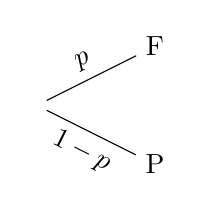
\begin{tikzpicture}[grow=right, sloped]
\node{}
child {node {P} edge from parent node[below] {$1-p$}}
child {node {F} edge from parent node[above] {$p$}};
\end{tikzpicture}
\end{center}

\section{Loi Binomiale}

\begin{definition}
La loi binomiale est une généralisation de la loi de Bernoulli qui
s'applique à une séquence de $n$ essais indépendants, chacun ayant une
probabilité de succès $p$. \\
Elle permet de modéliser le nombre total de succès obtenus parmi ces $n$ essais.
\end{definition}

\begin{propriete}
  \begin{enu}
  \item La loi binomiale est caractérisée par deux paramètres :
    \begin{itemize}
    \item $n$ : le nombre total d'essais.
    \item $p$ : la probabilité de succès pour chaque essai.
    \end{itemize}
  \item La variable aléatoire $X$ suivant la loi binomiale mesure le
    nombre de succès parmi les $n$ essais.
  \end{enu}
\end{propriete}

\begin{exercice}[0][Répétitions d’épreuves de Bernoulli]
On considère l'expérience suivante : \\
Une urne contient 3 boules blanches et 2 boules rouges. On tire au
hasard une boule et on la remet dans l'urne. \\
On répète l'expérience deux fois de suite.
\begin{enumerate}
\item Représenter l'ensemble des issues de ces expériences dans un arbre.
\item Déterminer les probabilités suivantes :
  \begin{enumerate}
  \item On tire deux boules blanches. 
  \item  On tire une boule blanche et une boule rouge. 
  \item  On tire au moins une boule blanche.
  \end{enumerate}
\end{enumerate}
\end{exercice}


\end{document}
%%% Local Variables:
%%% mode: LaTeX
%%% TeX-master: t
%%% End:
%% Font size %%
\documentclass[11pt]{article}

%% Load the custom package
\usepackage{Mathdoc}

%% Numéro de séquence %% Titre de la séquence %%
\renewcommand{\centerhead}{Fiche d'exercice suites géométrique}

%% Spacing commands %%
\renewcommand{\baselinestretch}{1}
\setlength{\parindent}{0pt}

\begin{document}

\section{Pourcentages d'évolutions}

\begin{multicols}{2}{2}
  \begin{exercice}
    \begin{enumerate}
    \item Dans une entreprise de $450$ salariés, il y a $24\,\%$ de
      cadres. \\Combien y a-t-il de cadres dans cette entreprise ?
    \item $1\,380$ personnes assistent à un concert. $60~\%$ ont moins
      de $18$ ans. \\Calculer le nombre de personnes mineures dans le
      public.
    \item Une réserve de protection d'oiseaux contient $2\,140$
      individus d'oiseaux. On dénombre $30~\%$ de pipits
      farlouse.\\Quel est le nombre de pipits farlouse ?
    \item Le cadeau commun que nous souhaitons faire à Nora coûte $40$
      €. Je participe à hauteur de $10~\%$ du prix total. \\Combien
      ai-je donné pour le cadeau de Nora ?
    \end{enumerate}
  \end{exercice}

  \begin{exercice}
    \begin{enumerate}
    \item Il y a 6 ans, la population d'une ville était de $82\,000$
      habitants. Depuis, elle a augmenté de $10~\%$. Calculer le
      nombre d'habitants actuel de cette ville.
    \item Un lycée avait $900$ élèves en 2023. Depuis, le nombre
      d'élèves a augmenté de $9~\%$. Calculer le nombre d'élèves dans
      ce lycée cette année.
    \item Un article coûtait $99$ €~et son prix a augmenté de
      $20~\%$. Calculer son nouveau prix.
    \item Le prix de mon ordinateur était de $750$ €~l'année dernière
      et il a augmenté de $12~\%$. Calculer son nouveau prix.
    \end{enumerate}
  \end{exercice}
\end{multicols}
\begin{exercice}
\begin{enumerate}
	\item Après une augmentation de $9~\%$ le prix de ma taxe d'habitation est maintenant $1\,315{,}63$ €. Calculer son prix avant l'augmentation.
	\item Depuis 2023 le nombre d'élèves d'un lycée a augmenté de $15~\%$. Il y a maintenant $483$ élèves. Calculer le nombre d'élèves en 2023 dans cet établissement.
	\item En 13 ans, la population d'une ville a diminué de $19~\%$ et est maintenant $129\,600$ habitants. Calculer sa population d'il y a 13 ans.
	\item Après une augmentation de $10~\%$ un article coûte maintenant $3{,}63$ €. Calculer son prix avant l'augmentation.
\end{enumerate}
\end{exercice}

\newpage

\section{Suites géométriques }

\begin{multicols}{2}
  \begin{exercice}
    \begin{enumerate}
    \item Soit $(w_n)$ une suite géométrique de raison $q$ définie
      pour tout $n\in \mathbb{N}$, telle que $w_0=7$ et $q=-3$.
      Donner l'expression de $w_n$ en fonction de $n$.
    \item Soit $(u_n)$ une suite géométrique de raison $q$ définie
      pour tout $n\in \mathbb{N}$, telle que $u_0=2$ et $q=-15$.
      Donner l'expression de $u_n$ en fonction de $n$.
    \item Soit $(w_n)$ une suite arithmétique de raison $r$ définie
      pour tout $n\in\mathbb{N}$, telle que $w_0=9$ et $r=2$.  Donner
      l'expression de $w_n$ en fonction de $n$.
    \item Soit $(v_n)$ une suite arithmétique de raison $r$ définie
      pour tout $n\in\mathbb{N}$, telle que $v_0=9$ et $r=14$.  Donner
      l'expression de $v_n$ en fonction de $n$.
    \end{enumerate}
  \end{exercice}

  \begin{exercice}
    \begin{enumerate}
    \item $(v_n)$ est une suite géométrique de raison $q=1{,}5$ et de premier terme $v_0=-10$.\\
      Calculer $v_{5}$.
    \item $(w_n)$ est une suite géométrique de raison $q=-1{,}6$ et de premier terme $w_0=-9$.\\
      Calculer $w_{10}$.
    \item $(w_n)$ est une suite géométrique de raison $q=-0{,}9$ et de premier terme $w_0=4$.\\
      Calculer $w_{6}$.
    \item $(v_n)$ est une suite géométrique de raison $q=1{,}4$ et de premier terme $v_0=-8$.\\
      Calculer $v_{7}$.
    \end{enumerate}
  \end{exercice}
\end{multicols}

\begin{exercice}
\begin{enumerate}
	\item Soit $w$ la suite géométrique de premier terme $w_1 = 9$ et de raison $0{,}4$.\\Calculer $\displaystyle S = w_1 + w_2 + ... + w_{12} =\sum_{k=1}^{12}w_k$ et donner un arrondi au millième près.
	\item Soit $w$ la suite géométrique de premier terme $w_1 = 2$ et de raison $0{,}4$.\\Calculer $\displaystyle S = w_1 + w_2 + ... + w_{10} =\sum_{k=1}^{10}w_k$ et donner un arrondi au millième près.
	\item Soit $v$ la suite géométrique de premier terme $v_0 = 10$ et de raison $1{,}9$.\\Calculer $\displaystyle S = v_0 + v_1 + ... + v_{12} =\sum_{k=0}^{12}v_k$ et donner un arrondi au millième près.
	\item Soit $w$ la suite géométrique de premier terme $w_0 = 10$ et de raison $0{,}3$.\\Calculer $\displaystyle S = w_0 + w_1 + ... + w_{12} =\sum_{k=0}^{12}w_k$ et donner un arrondi au millième près.
\end{enumerate}
\end{exercice}

\newpage

\section{Problèmes}

\begin{exercice}
Un entrepreneur décide d'investir une somme de 5 000 € dans un compte bancaire offrant un taux d'intérêt annuel de 4 \%.

\begin{enumerate}
    \item \textbf{Calcul du premier terme de la suite :}
    \begin{itemize}
        \item Au début de la première année, l'entrepreneur dépose 5 000 € sur son compte.
        \item À la fin de chaque année, les intérêts sont ajoutés au capital de départ.
    \end{itemize}

    \item \textbf{Modélisation de la suite :} Soit $u_n$ le capital au bout de $n$ années. Exprimez $u_{n+1}$ en fonction de $u_n$ et du taux d'intérêt. 
    \item \textbf{Terme explicite :} En déduire l'expression explicite de $u_n$ en fonction de $n$.
    \item \textbf{Évolution du capital :} Calculez le capital après 10
      ans.
    \item \textbf{Comparaison avec un autre taux d’intérêt :} \\
    Supposons qu'une autre banque offre un taux d’intérêt annuel de 5 \%.
    Calculez la valeur de l’investissement après 10 ans si le taux était de 5 \% au lieu de 4 \%, et comparez les deux évolutions.
\end{enumerate}
\end{exercice}

\begin{exercice}
Un entrepreneur souhaite financer un projet en mettant de côté une somme d'argent chaque mois. Il décide de commencer avec une somme de 200 € le premier mois et d'augmenter chaque mois le montant mis de côté de 5\,\% par rapport au mois précédent.

\begin{enumerate}
    \item \textbf{Détermination des termes de la suite :} \\
    Soit \( u_n \) la somme mise de côté le \( n \)-ième mois. Exprimez \( u_n \) en fonction de \( n \) et de \( u_1 \).
    
    \item \textbf{Expression de la somme des \( n \) premiers termes :} \\
    L'entrepreneur souhaite savoir combien il aura mis de côté au bout de \( n \) mois. Exprimez la somme \( S_n \) des \( n \) premiers termes de cette suite en fonction de \( n \), \( u_1 \) et du taux d’évolution.
    
    \item \textbf{Application numérique :} \\
    Calculez le montant total mis de côté au bout de 12 mois.
\end{enumerate}
\end{exercice}

\end{document}
%% Font size %%
\documentclass[11pt]{article}

%% Load the custom package
\usepackage{Mathdoc}

%% Numéro de séquence %% Titre de la séquence %%
\renewcommand{\centerhead}{}

%% Spacing commands %%
\renewcommand{\baselinestretch}{1}
\setlength{\parindent}{0pt}

\begin{document}

\section{Fonctions polynomiales}

\subsection{Polynômes de degré 2}

\subsection{Polynômes de degré 3 et plus}

\section{Nombre dérivé en un point}

\subsection{Équations de droites}

\subsection{Taux d'accroissement}

\subsection{Tangente à la courbe}

\section{Fonction dérivée}

\subsection{Definitions}

\subsection{Formules usuelles}

\subsection{Opérations}

\section{Applications}

\subsection{Sens de variation}

\subsection{Extremum}

\subsection{Convexité}

\end{document}
%% Font size %%
\documentclass[11pt]{article}

%% Load the custom package
\usepackage{Mathdoc}

%% Numéro de séquence %% Titre de la séquence %%
\renewcommand{\centerhead}{Chap. 4 : Polynôme du second degré - Discriminant}

%% Spacing commands %%
\renewcommand{\baselinestretch}{1}
\setlength{\parindent}{0pt}

\begin{document}

\section{Calcul de discriminant}

\begin{exercice}[0][Exercice Corrigé.]
\textbf{Calculer le discriminant de cette expression :}

 $A(x) = 5x^2-4x-1$

Correction : \\
\textit{
$\Delta_A = b^2 - 4 \times a \times c$ \\
$\Delta_A = \left(-4\right)^2-4\times5\times\left(-1\right)$ \\
$\Delta_A = 36$}
\end{exercice}

\begin{exercice}[1][Calculer le discriminant de chacune de ces expressions.]
  \begin{multicols}{2}
    \begin{enumerate}
    \item $A(x) = 5x^2+4x+2$ \\ \dtf \\ \dtf
    \item $B(x) = 2x^2+2x+4$ \\ \dtf \\ \dtf
    \item $C(x) = 5x^2+5x+4$ \\ \dtf \\ \dtf
    \item $D(x) = 5x^2+5x+5$ \\ \dtf \\ \dtf
    \end{enumerate}
  \end{multicols}
\end{exercice}

\begin{exercice}[2][Calculer le discriminant de chacune de ces expressions.]
  \begin{multicols}{2}
    \begin{enumerate}
    \item $A(x) = -2x^2+2x+1$ \\ \dtf \\ \dtf
    \item $B(x) = -3x^2+5$ \\ \dtf \\ \dtf
    \item $C(x) = -3x^2-3x-5$ \\ \dtf \\ \dtf
    \item $D(x) = -3x^2+x-1$ \\ \dtf \\ \dtf
    \end{enumerate}
  \end{multicols}
\end{exercice}

\begin{exercice}[3][Calculer le discriminant de chacune de ces expressions.]
  \begin{multicols}{2}
    \begin{enumerate}
    \item $A(x) = -x^2+\dfrac{1}{2}x$ \\ \dtf \\ \dtf \\ \dtf
    \item $B(x) = -\dfrac{6}{2}x^2-\dfrac{9}{2}x+\dfrac{2}{3}$ \\ \dtf
      \\ \dtf \\ \dtf
    \item $C(x) = -\dfrac{5}{3}x-\dfrac{6}{5}$ \\ \dtf \\ \dtf
    \item $D(x) = -\dfrac{7}{5}x^2+\dfrac{1}{3}x+\dfrac{7}{5}$ \\ \dtf
      \\ \dtf \\ \dtf
    \end{enumerate}
  \end{multicols}
\end{exercice}

\newpage

\section{Déterminer le nombre de solutions}

\begin{exercice}[0][Exercice Corrigé.]
\textbf{Calculer le discriminant et déterminer le nombre de solutions de cette
équation dans $\mathbb{R}$.} \\
$2x^2-1=0$

Correction :\\
\begin{minipage}[t]{\linewidth}$\Delta = 0^2-4\times2\times(-1)=8$\\$\Delta>0$ \textit{donc l'équation admet \underline{deux solutions}}.\end{minipage}
\end{exercice}

\begin{exercice}[1][Nombre de solutions.]
Calculer le discriminant et déterminer le nombre de solutions de cette
équation dans $\mathbb{R}$.
\begin{multicols}{2}
  \begin{enumerate}
  \item $x^2-x-2=0$ \\ \dtf \\ \dtf
  \item $-7x-3x^2-9=0$ \\ \dtf \\ \dtf
  \item $-x-6+x^2=0$ \\ \dtf \\ \dtf
  \item $-10x^2-x-9=0$ \\ \dtf \\ \dtf
  \end{enumerate}
\end{multicols}
\end{exercice}

\begin{exercice}[2][Nombre de solutions.]
Calculer le discriminant et déterminer le nombre de solutions de cette
équation dans $\mathbb{R}$.
\begin{multicols}{2}
  \begin{enumerate}
  \item $-16+8x-x^2=0$ \\ \dtf \\ \dtf
  \item $x^2+13x+40=0$ \\ \dtf \\ \dtf
  \item $-2-9x^2+x=0$ \\ \dtf \\ \dtf
  \item $7x^2-5x+6=0$ \\ \dtf \\ \dtf
  \end{enumerate}
\end{multicols}
\end{exercice}

\begin{exercice}[3][Nombre de solutions.]
Calculer le discriminant et déterminer le nombre de solutions de cette
équation dans $\mathbb{R}$.
\begin{multicols}{2}
  \begin{enumerate}
  \item $-2x^2-\dfrac{32}{25}+\dfrac{16}{5}x=0$ \\ \dtf \\ \dtf \\ \dtf 
  \item $-5x^2+8x+6=0$ \\ \dtf \\ \dtf \\ \dtf 
  \item $-2x^2-10=0$ \\ \dtf \\ \dtf \\ \dtf 
  \item $-10x^2+2x-8=0$ \\ \dtf \\ \dtf \\ \dtf 
  \end{enumerate}
\end{multicols}
\end{exercice}

\newpage

\section{Résolution d'équation}

\begin{exercice}
\textbf{Résoudre l'équation suivante.}\\
 $x^2-2x-3=0$ \\
Correction :\\
\textit{On calcule le discriminant :} \\
\[\Delta=\left(-2\right)^2-4\times1\times\left(-3\right)=16.\] \\
\textit{On a $\Delta=16$, donc l'équation a \underline{deux solutions}. \\
Les solutions sont données par la formule :
}\[x_{1,2}=\dfrac{-b \pm \sqrt{\Delta}}{2\times a}\]
\textit{Donc :}
\[x_{1}=\dfrac{-\left(-2\right)+\sqrt{16}}{2\times1} \quad
x_{2}=\dfrac{-\left(-2\right)-\sqrt{16}}{2\times1}\]\\
\textit{En calculant, on obtient} ${S = \left\{-1;3\right\}}$.
\end{exercice}


\begin{exercice}[1][Résoudre les équations suivantes.]
\begin{multicols}{2}
  $x^2+2x+1=0$  \\ \\ \encart{3cm}
  $x^2-4x=0$ \\ \\ \encart{3cm}
\end{multicols}
\end{exercice}

\begin{exercice}[2][Résoudre les équations suivantes.]
\begin{multicols}{2}
$15x+56+x^2=0$ \\ \\ \encart{3cm}
$-7x^2-2-7x=0$ \\ \\ \encart{3cm}
\end{multicols}
\end{exercice}

\newpage

\begin{exercice}[2][Résoudre les équations suivantes.]
\begin{multicols}{2}
$40x-200=2x^2$ \\ \\ \encart{3cm}
$-x=-x^2+42$ \\ \\ \encart{3cm}
\end{multicols}
\end{exercice}

\begin{exercice}[3][Résoudre les équations suivantes.]
\begin{multicols}{2}
$-14x-\dfrac{49}{2}-2x^2=0$ \\ \\ \encart{3cm}
$\dfrac{3}{2}x^2-\dfrac{63}{100}+\dfrac{33}{20}x=0$ \\ \\ \encart{3cm}
\end{multicols}
\end{exercice}

\begin{exercice}[3][Résoudre les équations suivantes.]
\begin{multicols}{2}
$3x^2-\dfrac{60}{3}x=-\dfrac{300}{9}$ \\ \\ \encart{3cm}
$-3x^2=\dfrac{141}{6}x-\dfrac{189}{6}$ \\ \\ \encart{3cm}
\end{multicols}
\end{exercice}

\begin{exercice}[4][Résoudre les équations suivantes.]
\begin{multicols}{2}
 $-\dfrac{69}{3}x+\dfrac{297}{9}+\dfrac{10}{3}x^2=-\dfrac{1}{3}-3x+\dfrac{1}{3}x^2$ \\ \\ \encart{3cm}
  $\dfrac{2}{3}x^2+\dfrac{8}{4}x=4x-\dfrac{4}{3}x^2-\dfrac{1}{2}$ \\ \\ \encart{3cm}
\end{multicols}
\end{exercice}

\end{document}
%% Font size %%
\documentclass[11pt]{article}

%% Load the custom package
\usepackage{Mathdoc}

%% Numéro de séquence %% Titre de la séquence %%
\renewcommand{\centerhead}{Chap. 4 : Tableau de variation}

%% Spacing commands %%
\renewcommand{\baselinestretch}{1}
\setlength{\parindent}{0pt}

\begin{document}

\begin{exercice}[0][Exercice corrigé.]
Dresser le tableau de signes de la fonction $f$ définie sur  $\mathbb
R$ par : $f(x)=-4x^2+16x+20$, sachant que $x_1=5$ et $x_2=-1$. \\
Ici, $a=-4$, donc la fonction est "en forme de cloche", elle est
\underline{négative} puis \underline{positive} et enfin \underline{négative}. \\
Donc le tableau de signes de $f$ sur $\mathbb{R}$  est :
\begin{center}
\begin{tikzpicture}[baseline, scale=0.75]
\tkzTabInit[lgt=3,deltacl=0.8,espcl=2.1]{ $x$ / 1.5, $f(x)$ / 1.5}{
  $-\infty$, $-1$, $5$, $+\infty$} \tkzTabLine{ , -, z, +, z, -}
\end{tikzpicture}
\end{center}
\end{exercice}

\end{document}
%% Font size %%
\documentclass[11pt]{article}

%% Load the custom package
\usepackage{Mathdoc}

%% Numéro de séquence %% Titre de la séquence %%
\renewcommand{\centerhead}{Chap. 4 : Tableau de variation}

%% Spacing commands %%
\renewcommand{\baselinestretch}{1}
\setlength{\parindent}{0pt}

\begin{document}

\begin{exercice}[0][Exercice corrigé.]
\textbf{Dresser le tableau de signes de la fonction $f$ définie sur  $\mathbb
R$ par $f(x)=5x-4$, \\ sachant que $f(\dfrac{4}{5})=0$ ?} \\ \\
Le coefficient directeur de la fonction est $a=5$. \\
Donc $5>0~$, $~f(x)$ est \underline{négative} puis \underline{positive}. \\
On obtient le tableau de variation suivant :
\begin{center}
  \begin{tikzpicture}[baseline, scale=0.60]
    \tkzTabInit[lgt=5,deltacl=0.8,espcl=5]{ $x$ / 2, $f(x)$ / 2}{
      $-\infty$, $\dfrac{4}{5}$, $+\infty$} \tkzTabLine{ , -, z, +}
  \end{tikzpicture}
\end{center}
\end{exercice}

\begin{exercice}[1][Tableau de variations en connaissant la racine.]
\textbf{Dresser le tableau de signes de la fonction $f$ définie sur  $\mathbb
R$ par $f(x)=10x-5$, \\ sachant que $f(\dfrac{1}{2})=0$ ?} \\ \\
Le coefficient directeur de la fonction est \ldots\ldots\ldots\ldots \\
Donc \dotfill \\
On obtient le tableau de variation suivant :
\begin{center}
  \begin{tikzpicture}[baseline, scale=0.60]
    \tkzTabInit[lgt=5,deltacl=0.8,espcl=5]{ $x$ / 2, $f(x)$ / 2}{
      $-\infty$, \ldots\ldots\ldots, $+\infty$} \tkzTabLine{ , , z, }
  \end{tikzpicture}
\end{center}
\end{exercice}

\begin{exercice}[1][Tableau de variations en connaissant la racine.]
\textbf{Dresser le tableau de signes de la fonction $f$ définie sur  $\mathbb
R$ par $f(x)=-3x+6$, \\ sachant que $f(2)=0$ ?} \\ \\
Le coefficient directeur de la fonction est \ldots\ldots\ldots\ldots \\
Donc \dotfill \\
On obtient le tableau de variation suivant :
\begin{center}
  \begin{tikzpicture}[baseline, scale=0.60]
    \tkzTabInit[lgt=5,deltacl=0.8,espcl=5]{ $x$ / 2, $f(x)$ / 2}{
      $-\infty$, \ldots\ldots\ldots, $+\infty$} \tkzTabLine{ , , z, }
  \end{tikzpicture}
\end{center}
\end{exercice}

%\newpage

\begin{exercice}[0][Exercice corrigé.]
Résoudre l'équation suivante. \\
$6x+8=0$\\
$6x=-8$ \\
$x=\dfrac{-8}{6}$\\
$x=\dfrac{-4}{3}$\\
La solution de l'équation $6x+8=0$ est $x_0=-\dfrac{4}{3}$.
\end{exercice}

\begin{exercice}[1][Résoudre les équations suivantes.]
\begin{multicols}{2}
\begin{enumerate}
\item $-7x-12=0$ \\ \\ \encart{3cm}
\item $-12x+8=0$ \\ \\ \encart{3cm}
\item $11x-2=0$ \\ \\ \encart{3cm}
\item $12x-4=0$ \\ \\ \encart{3cm}
\end{enumerate}
\end{multicols}
\end{exercice}

\begin{exercice}[2][Résoudre les équations suivantes.]
\begin{multicols}{2}
\begin{enumerate}
\item $7x+3=10x-8$ \\ \\ \encart{4cm}
\item $-2x+13=7x-10$ \\ \\ \encart{4cm}
\end{enumerate}
\end{multicols}
\end{exercice}

%\newpage

\begin{exercice}[0][Exercice corrigé.]
\textbf{Dresser le tableau de signes de la fonction $f$ définie sur  $\mathbb
R$ par $f(x)=2x-5$ ?} \\
On résoud : $2x-5=0$ $\iff$ $2x=5$ $\iff$ $x=\dfrac{5}{2}$ \\
Le coefficient directeur de $f$ est $a=2$, donc $f$ est négative puis
poisitive. \\
On dresse le tableau de variation suivant :
\begin{center}
  \begin{tikzpicture}[baseline, scale=0.75]
    \tkzTabInit[lgt=5,deltacl=0.8,espcl=5]{ $x$ / 2, $f(x)$ / 2}{
      $-\infty$, $\dfrac{5}{2}$, $+\infty$} \tkzTabLine{ ,- , z,+ }
  \end{tikzpicture}
\end{center}
\end{exercice}

\begin{exercice}[1][Dresser un tableau de variation.]
\textbf{Dresser le tableau de signes de la fonction $f$ définie sur  $\mathbb
R$ par $f(x)=-x+4$ ?} \\
\dtf \\ \dtf \\ \dtf \\ \dtf \\ \dtf
\begin{center}
  \begin{tikzpicture}[baseline, scale=0.60]
    \tkzTabInit[lgt=5,deltacl=0.8,espcl=5]{ $x$ / 2, $f(x)$ / 2}{
      $-\infty$, $\ldots\ldots\ldots$, $+\infty$} \tkzTabLine{ , , z, }
  \end{tikzpicture}
\end{center}
\end{exercice}

\begin{multicols}{2}
\begin{exercice}[2][Dresser un tableau de variation.]
\textbf{Dresser le tableau de signes de la fonction $f$ définie sur  $\mathbb
R$ par \\ $f(x)=12x+8$} \\
\dtf \\ \dtf \\ \dtf \\ \dtf \\ \dtf \\ \dtf
\begin{center}
  \begin{tikzpicture}[baseline, scale=0.35]
    \tkzTabInit[lgt=5,deltacl=0.8,espcl=5]{ $x$ / 2, $f(x)$ / 2}{
      , ,} \tkzTabLine{ , , , }
  \end{tikzpicture}
\end{center}
\end{exercice}

\begin{exercice}[2][Dresser un tableau de variation.]
\textbf{Dresser le tableau de signes de la fonction $f$ définie sur  $\mathbb
R$ par \\ $f(x)=-3x-6$} \\
\dtf \\ \dtf \\ \dtf \\ \dtf \\ \dtf  \\ \dtf
\begin{center}
  \begin{tikzpicture}[baseline, scale=0.35]
    \tkzTabInit[lgt=5,deltacl=0.8,espcl=5]{ $x$ / 2, $f(x)$ / 2}{
      , ,} \tkzTabLine{ , , , }
  \end{tikzpicture}
\end{center}
\end{exercice}
\end{multicols}

\begin{exercice}[2][\underline{Sur le cahiers}, dresser les tableaux de signes.]
\begin{multicols}{2}
\begin{enumerate}
\item  $f(x)=2x-4$ 
\item  $f(x)=x-5$ 
\item  $f(x)=4x+4$ 
\item  $f(x)=4x-6$ 
\item  $f(x)=-x+6$ 
\item  $f(x)=6x+1$ 
\end{enumerate}
\end{multicols}
\end{exercice}

\begin{exercice}[3][\underline{Sur le cahiers}, dresser les tableaux de signes.]
\begin{multicols}{2}
\begin{enumerate}
	\item  $f(x)=-\dfrac{10}{9}x+4$
	\item  $g(x)=-\dfrac{8}{7}x+6$
	\item  $h(x)=-\dfrac{6}{5}x-9$
	\item  $i(x)=-\dfrac{6}{5}x-2$
	\item  $j(x)=\dfrac{8}{7}x+6$
	\item  $k(x)=-\dfrac{6}{5}x-4$
\end{enumerate}
\end{multicols}
\end{exercice}

\begin{exercice}[2][Tableaux de signes à partir d'un graphique.]
\begin{multicols}{2}
\begin{enumerate}[itemsep=1em]
	\item \begin{minipage}[t]{\linewidth} Dresser le tableau de signes de la fonction $f$ représentée ci-dessous.\\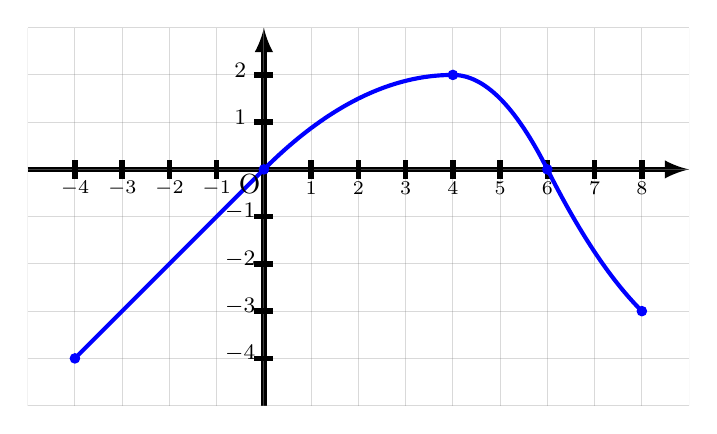
\begin{tikzpicture}[baseline,scale = 0.6]

    \tikzset{
      point/.style={
        thick,
        draw,
        cross out,
        inner sep=0pt,
        minimum width=5pt,
        minimum height=5pt,
      },
    }
    \clip (-5,-5) rectangle (9,3);
    	\draw[color ={black},line width = 2,>=latex,->] (-5,0)--(9,0);
	\draw[color ={black},line width = 2,>=latex,->] (0,-5)--(0,3);
	\draw[color ={gray},opacity = 0.3] (-5,0)--(9,0);
	\draw[color ={gray},opacity = 0.3] (-5,1)--(9,1);
	\draw[color ={gray},opacity = 0.3] (-5,2)--(9,2);
	\draw[color ={gray},opacity = 0.3] (-5,3)--(9,3);
	\draw[color ={gray},opacity = 0.3] (-5,0)--(9,0);
	\draw[color ={gray},opacity = 0.3] (-5,-1)--(9,-1);
	\draw[color ={gray},opacity = 0.3] (-5,-2)--(9,-2);
	\draw[color ={gray},opacity = 0.3] (-5,-3)--(9,-3);
	\draw[color ={gray},opacity = 0.3] (-5,-4)--(9,-4);
	\draw[color ={gray},opacity = 0.3] (-5,-5)--(9,-5);
	\draw[color ={gray},opacity = 0.3] (0,-5)--(0,3);
	\draw[color ={gray},opacity = 0.3] (1,-5)--(1,3);
	\draw[color ={gray},opacity = 0.3] (2,-5)--(2,3);
	\draw[color ={gray},opacity = 0.3] (3,-5)--(3,3);
	\draw[color ={gray},opacity = 0.3] (4,-5)--(4,3);
	\draw[color ={gray},opacity = 0.3] (5,-5)--(5,3);
	\draw[color ={gray},opacity = 0.3] (6,-5)--(6,3);
	\draw[color ={gray},opacity = 0.3] (7,-5)--(7,3);
	\draw[color ={gray},opacity = 0.3] (8,-5)--(8,3);
	\draw[color ={gray},opacity = 0.3] (9,-5)--(9,3);
	\draw[color ={gray},opacity = 0.3] (0,-5)--(0,3);
	\draw[color ={gray},opacity = 0.3] (-1,-5)--(-1,3);
	\draw[color ={gray},opacity = 0.3] (-2,-5)--(-2,3);
	\draw[color ={gray},opacity = 0.3] (-3,-5)--(-3,3);
	\draw[color ={gray},opacity = 0.3] (-4,-5)--(-4,3);
	\draw[color ={gray},opacity = 0.3] (-5,-5)--(-5,3);
	\draw[color ={black},line width = 2] (1,-0.2)--(1,0.2);
	\draw[color ={black},line width = 2] (2,-0.2)--(2,0.2);
	\draw[color ={black},line width = 2] (3,-0.2)--(3,0.2);
	\draw[color ={black},line width = 2] (4,-0.2)--(4,0.2);
	\draw[color ={black},line width = 2] (5,-0.2)--(5,0.2);
	\draw[color ={black},line width = 2] (6,-0.2)--(6,0.2);
	\draw[color ={black},line width = 2] (7,-0.2)--(7,0.2);
	\draw[color ={black},line width = 2] (8,-0.2)--(8,0.2);
	\draw[color ={black},line width = 2] (-1,-0.2)--(-1,0.2);
	\draw[color ={black},line width = 2] (-2,-0.2)--(-2,0.2);
	\draw[color ={black},line width = 2] (-3,-0.2)--(-3,0.2);
	\draw[color ={black},line width = 2] (-4,-0.2)--(-4,0.2);
	\draw[color ={black},line width = 2] (-0.2,1)--(0.2,1);
	\draw[color ={black},line width = 2] (-0.2,2)--(0.2,2);
	\draw[color ={black},line width = 2] (-0.2,-1)--(0.2,-1);
	\draw[color ={black},line width = 2] (-0.2,-2)--(0.2,-2);
	\draw[color ={black},line width = 2] (-0.2,-3)--(0.2,-3);
	\draw[color ={black},line width = 2] (-0.2,-4)--(0.2,-4);
	\draw (1,-0.4) node[anchor = center] {\scriptsize \color{black}{$1$}};
	\draw (2,-0.4) node[anchor = center] {\scriptsize \color{black}{$2$}};
	\draw (3,-0.4) node[anchor = center] {\scriptsize \color{black}{$3$}};
	\draw (4,-0.4) node[anchor = center] {\scriptsize \color{black}{$4$}};
	\draw (5,-0.4) node[anchor = center] {\scriptsize \color{black}{$5$}};
	\draw (6,-0.4) node[anchor = center] {\scriptsize \color{black}{$6$}};
	\draw (7,-0.4) node[anchor = center] {\scriptsize \color{black}{$7$}};
	\draw (8,-0.4) node[anchor = center] {\scriptsize \color{black}{$8$}};
	\draw (-1,-0.4) node[anchor = center] {\scriptsize \color{black}{$-1$}};
	\draw (-2,-0.4) node[anchor = center] {\scriptsize \color{black}{$-2$}};
	\draw (-3,-0.4) node[anchor = center] {\scriptsize \color{black}{$-3$}};
	\draw (-4,-0.4) node[anchor = center] {\scriptsize \color{black}{$-4$}};
	\draw (-0.5,1.1) node[anchor = center] {\footnotesize \color{black}{$1$}};
	\draw (-0.5,2.1) node[anchor = center] {\footnotesize \color{black}{$2$}};
	\draw (-0.5,-0.9) node[anchor = center] {\footnotesize \color{black}{$-1$}};
	\draw (-0.5,-1.9) node[anchor = center] {\footnotesize \color{black}{$-2$}};
	\draw (-0.5,-2.9) node[anchor = center] {\footnotesize \color{black}{$-3$}};
	\draw (-0.5,-3.9) node[anchor = center] {\footnotesize \color{black}{$-4$}};
	
	\draw[color = {blue},line width = 1.5, opacity = 1](-4,-4) .. controls +(1.33,1.33) and +(-1.33,-1.33)  .. (0.00,0.00)
 .. controls +(1.33,1.33) and +(-1.33,0.00)  .. (4.00,2.00)
 .. controls +(0.67,0.00) and +(-0.67,1.33)  .. (6.00,0.00)
 .. controls +(0.67,-1.33) and +(-0.67,0.67)  .. (8.00,-3.00)
;

	 \filldraw[color={blue},fill={{blue}}] (-4,-4) circle (0.1);
	 \filldraw[color={blue},fill={{blue}}] (0,0) circle (0.1);
	 \filldraw[color={blue},fill={{blue}}] (4,2) circle (0.1);
	 \filldraw[color={blue},fill={{blue}}] (6,0) circle (0.1);
	 \filldraw[color={blue},fill={{blue}}] (8,-3) circle (0.1);
	\draw [color={black}] (-0.3,-0.3) node[anchor = center,scale=1, rotate = 0] {O};

\end{tikzpicture} \end{minipage}
	\item \begin{minipage}[t]{\linewidth} Dresser le tableau de signes de la fonction $f$ représentée ci-dessous.\\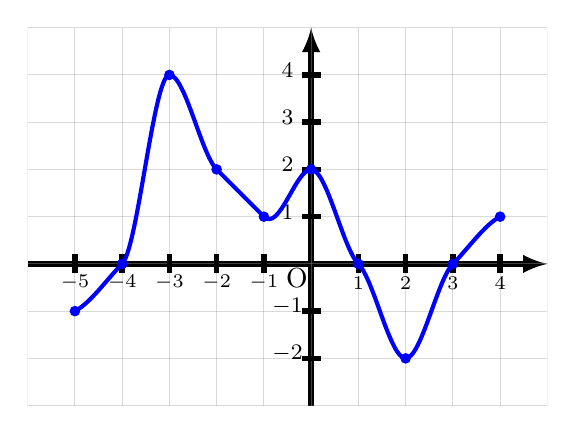
\begin{tikzpicture}[baseline,scale = 0.6]

    \tikzset{
      point/.style={
        thick,
        draw,
        cross out,
        inner sep=0pt,
        minimum width=5pt,
        minimum height=5pt,
      },
    }
    \clip (-6,-3) rectangle (5,5);
    	\draw[color ={black},line width = 2,>=latex,->] (-6,0)--(5,0);
	\draw[color ={black},line width = 2,>=latex,->] (0,-3)--(0,5);
	\draw[color ={gray},opacity = 0.3] (-6,0)--(5,0);
	\draw[color ={gray},opacity = 0.3] (-6,1)--(5,1);
	\draw[color ={gray},opacity = 0.3] (-6,2)--(5,2);
	\draw[color ={gray},opacity = 0.3] (-6,3)--(5,3);
	\draw[color ={gray},opacity = 0.3] (-6,4)--(5,4);
	\draw[color ={gray},opacity = 0.3] (-6,5)--(5,5);
	\draw[color ={gray},opacity = 0.3] (-6,0)--(5,0);
	\draw[color ={gray},opacity = 0.3] (-6,-1)--(5,-1);
	\draw[color ={gray},opacity = 0.3] (-6,-2)--(5,-2);
	\draw[color ={gray},opacity = 0.3] (-6,-3)--(5,-3);
	\draw[color ={gray},opacity = 0.3] (0,-3)--(0,5);
	\draw[color ={gray},opacity = 0.3] (1,-3)--(1,5);
	\draw[color ={gray},opacity = 0.3] (2,-3)--(2,5);
	\draw[color ={gray},opacity = 0.3] (3,-3)--(3,5);
	\draw[color ={gray},opacity = 0.3] (4,-3)--(4,5);
	\draw[color ={gray},opacity = 0.3] (5,-3)--(5,5);
	\draw[color ={gray},opacity = 0.3] (0,-3)--(0,5);
	\draw[color ={gray},opacity = 0.3] (-1,-3)--(-1,5);
	\draw[color ={gray},opacity = 0.3] (-2,-3)--(-2,5);
	\draw[color ={gray},opacity = 0.3] (-3,-3)--(-3,5);
	\draw[color ={gray},opacity = 0.3] (-4,-3)--(-4,5);
	\draw[color ={gray},opacity = 0.3] (-5,-3)--(-5,5);
	\draw[color ={gray},opacity = 0.3] (-6,-3)--(-6,5);
	\draw[color ={black},line width = 2] (1,-0.2)--(1,0.2);
	\draw[color ={black},line width = 2] (2,-0.2)--(2,0.2);
	\draw[color ={black},line width = 2] (3,-0.2)--(3,0.2);
	\draw[color ={black},line width = 2] (4,-0.2)--(4,0.2);
	\draw[color ={black},line width = 2] (-1,-0.2)--(-1,0.2);
	\draw[color ={black},line width = 2] (-2,-0.2)--(-2,0.2);
	\draw[color ={black},line width = 2] (-3,-0.2)--(-3,0.2);
	\draw[color ={black},line width = 2] (-4,-0.2)--(-4,0.2);
	\draw[color ={black},line width = 2] (-5,-0.2)--(-5,0.2);
	\draw[color ={black},line width = 2] (-0.2,1)--(0.2,1);
	\draw[color ={black},line width = 2] (-0.2,2)--(0.2,2);
	\draw[color ={black},line width = 2] (-0.2,3)--(0.2,3);
	\draw[color ={black},line width = 2] (-0.2,4)--(0.2,4);
	\draw[color ={black},line width = 2] (-0.2,-1)--(0.2,-1);
	\draw[color ={black},line width = 2] (-0.2,-2)--(0.2,-2);
	\draw (1,-0.4) node[anchor = center] {\scriptsize \color{black}{$1$}};
	\draw (2,-0.4) node[anchor = center] {\scriptsize \color{black}{$2$}};
	\draw (3,-0.4) node[anchor = center] {\scriptsize \color{black}{$3$}};
	\draw (4,-0.4) node[anchor = center] {\scriptsize \color{black}{$4$}};
	\draw (-1,-0.4) node[anchor = center] {\scriptsize \color{black}{$-1$}};
	\draw (-2,-0.4) node[anchor = center] {\scriptsize \color{black}{$-2$}};
	\draw (-3,-0.4) node[anchor = center] {\scriptsize \color{black}{$-3$}};
	\draw (-4,-0.4) node[anchor = center] {\scriptsize \color{black}{$-4$}};
	\draw (-5,-0.4) node[anchor = center] {\scriptsize \color{black}{$-5$}};
	\draw (-0.5,1.1) node[anchor = center] {\footnotesize \color{black}{$1$}};
	\draw (-0.5,2.1) node[anchor = center] {\footnotesize \color{black}{$2$}};
	\draw (-0.5,3.1) node[anchor = center] {\footnotesize \color{black}{$3$}};
	\draw (-0.5,4.1) node[anchor = center] {\footnotesize \color{black}{$4$}};
	\draw (-0.5,-0.9) node[anchor = center] {\footnotesize \color{black}{$-1$}};
	\draw (-0.5,-1.9) node[anchor = center] {\footnotesize \color{black}{$-2$}};
	
	\draw[color = {blue},line width = 1.5, opacity = 1](-5,-1) .. controls +(0.33,0.17) and +(-0.33,-0.33)  .. (-4.00,0.00)
 .. controls +(0.33,0.33) and +(-0.33,0.00)  .. (-3.00,4.00)
 .. controls +(0.33,0.00) and +(-0.33,0.33)  .. (-2.00,2.00)
 .. controls +(0.33,-0.33) and +(-0.33,0.33)  .. (-1.00,1.00)
 .. controls +(0.33,-0.33) and +(-0.33,0.00)  .. (0.00,2.00)
 .. controls +(0.33,0.00) and +(-0.33,0.33)  .. (1.00,0.00)
 .. controls +(0.33,-0.33) and +(-0.33,0.00)  .. (2.00,-2.00)
 .. controls +(0.33,0.00) and +(-0.33,-0.33)  .. (3.00,0.00)
 .. controls +(0.33,0.33) and +(-0.33,-0.17)  .. (4.00,1.00)
;

	 \filldraw[color={blue},fill={{blue}}] (-5,-1) circle (0.1);
	 \filldraw[color={blue},fill={{blue}}] (-4,0) circle (0.1);
	 \filldraw[color={blue},fill={{blue}}] (-3,4) circle (0.1);
	 \filldraw[color={blue},fill={{blue}}] (-2,2) circle (0.1);
	 \filldraw[color={blue},fill={{blue}}] (-1,1) circle (0.1);
	 \filldraw[color={blue},fill={{blue}}] (0,2) circle (0.1);
	 \filldraw[color={blue},fill={{blue}}] (1,0) circle (0.1);
	 \filldraw[color={blue},fill={{blue}}] (2,-2) circle (0.1);
	 \filldraw[color={blue},fill={{blue}}] (3,0) circle (0.1);
	 \filldraw[color={blue},fill={{blue}}] (4,1) circle (0.1);
	\draw [color={black}] (-0.3,-0.3) node[anchor = center,scale=1, rotate = 0] {O};

\end{tikzpicture} \end{minipage}
	\item \begin{minipage}[t]{\linewidth} Dresser le tableau de signes de la fonction $f$ représentée ci-dessous.\\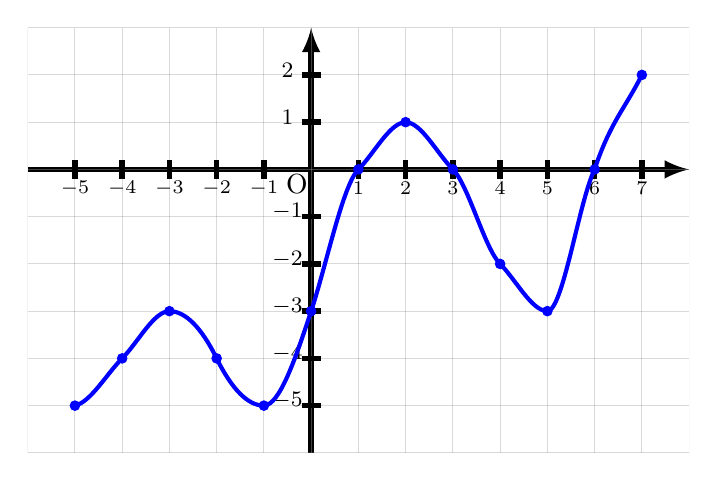
\begin{tikzpicture}[baseline,scale = 0.6]

    \tikzset{
      point/.style={
        thick,
        draw,
        cross out,
        inner sep=0pt,
        minimum width=5pt,
        minimum height=5pt,
      },
    }
    \clip (-6,-6) rectangle (8,3);
    	\draw[color ={black},line width = 2,>=latex,->] (-6,0)--(8,0);
	\draw[color ={black},line width = 2,>=latex,->] (0,-6)--(0,3);
	\draw[color ={gray},opacity = 0.3] (-6,0)--(8,0);
	\draw[color ={gray},opacity = 0.3] (-6,1)--(8,1);
	\draw[color ={gray},opacity = 0.3] (-6,2)--(8,2);
	\draw[color ={gray},opacity = 0.3] (-6,3)--(8,3);
	\draw[color ={gray},opacity = 0.3] (-6,0)--(8,0);
	\draw[color ={gray},opacity = 0.3] (-6,-1)--(8,-1);
	\draw[color ={gray},opacity = 0.3] (-6,-2)--(8,-2);
	\draw[color ={gray},opacity = 0.3] (-6,-3)--(8,-3);
	\draw[color ={gray},opacity = 0.3] (-6,-4)--(8,-4);
	\draw[color ={gray},opacity = 0.3] (-6,-5)--(8,-5);
	\draw[color ={gray},opacity = 0.3] (-6,-6)--(8,-6);
	\draw[color ={gray},opacity = 0.3] (0,-6)--(0,3);
	\draw[color ={gray},opacity = 0.3] (1,-6)--(1,3);
	\draw[color ={gray},opacity = 0.3] (2,-6)--(2,3);
	\draw[color ={gray},opacity = 0.3] (3,-6)--(3,3);
	\draw[color ={gray},opacity = 0.3] (4,-6)--(4,3);
	\draw[color ={gray},opacity = 0.3] (5,-6)--(5,3);
	\draw[color ={gray},opacity = 0.3] (6,-6)--(6,3);
	\draw[color ={gray},opacity = 0.3] (7,-6)--(7,3);
	\draw[color ={gray},opacity = 0.3] (8,-6)--(8,3);
	\draw[color ={gray},opacity = 0.3] (0,-6)--(0,3);
	\draw[color ={gray},opacity = 0.3] (-1,-6)--(-1,3);
	\draw[color ={gray},opacity = 0.3] (-2,-6)--(-2,3);
	\draw[color ={gray},opacity = 0.3] (-3,-6)--(-3,3);
	\draw[color ={gray},opacity = 0.3] (-4,-6)--(-4,3);
	\draw[color ={gray},opacity = 0.3] (-5,-6)--(-5,3);
	\draw[color ={gray},opacity = 0.3] (-6,-6)--(-6,3);
	\draw[color ={black},line width = 2] (1,-0.2)--(1,0.2);
	\draw[color ={black},line width = 2] (2,-0.2)--(2,0.2);
	\draw[color ={black},line width = 2] (3,-0.2)--(3,0.2);
	\draw[color ={black},line width = 2] (4,-0.2)--(4,0.2);
	\draw[color ={black},line width = 2] (5,-0.2)--(5,0.2);
	\draw[color ={black},line width = 2] (6,-0.2)--(6,0.2);
	\draw[color ={black},line width = 2] (7,-0.2)--(7,0.2);
	\draw[color ={black},line width = 2] (-1,-0.2)--(-1,0.2);
	\draw[color ={black},line width = 2] (-2,-0.2)--(-2,0.2);
	\draw[color ={black},line width = 2] (-3,-0.2)--(-3,0.2);
	\draw[color ={black},line width = 2] (-4,-0.2)--(-4,0.2);
	\draw[color ={black},line width = 2] (-5,-0.2)--(-5,0.2);
	\draw[color ={black},line width = 2] (-0.2,1)--(0.2,1);
	\draw[color ={black},line width = 2] (-0.2,2)--(0.2,2);
	\draw[color ={black},line width = 2] (-0.2,-1)--(0.2,-1);
	\draw[color ={black},line width = 2] (-0.2,-2)--(0.2,-2);
	\draw[color ={black},line width = 2] (-0.2,-3)--(0.2,-3);
	\draw[color ={black},line width = 2] (-0.2,-4)--(0.2,-4);
	\draw[color ={black},line width = 2] (-0.2,-5)--(0.2,-5);
	\draw (1,-0.4) node[anchor = center] {\scriptsize \color{black}{$1$}};
	\draw (2,-0.4) node[anchor = center] {\scriptsize \color{black}{$2$}};
	\draw (3,-0.4) node[anchor = center] {\scriptsize \color{black}{$3$}};
	\draw (4,-0.4) node[anchor = center] {\scriptsize \color{black}{$4$}};
	\draw (5,-0.4) node[anchor = center] {\scriptsize \color{black}{$5$}};
	\draw (6,-0.4) node[anchor = center] {\scriptsize \color{black}{$6$}};
	\draw (7,-0.4) node[anchor = center] {\scriptsize \color{black}{$7$}};
	\draw (-1,-0.4) node[anchor = center] {\scriptsize \color{black}{$-1$}};
	\draw (-2,-0.4) node[anchor = center] {\scriptsize \color{black}{$-2$}};
	\draw (-3,-0.4) node[anchor = center] {\scriptsize \color{black}{$-3$}};
	\draw (-4,-0.4) node[anchor = center] {\scriptsize \color{black}{$-4$}};
	\draw (-5,-0.4) node[anchor = center] {\scriptsize \color{black}{$-5$}};
	\draw (-0.5,1.1) node[anchor = center] {\footnotesize \color{black}{$1$}};
	\draw (-0.5,2.1) node[anchor = center] {\footnotesize \color{black}{$2$}};
	\draw (-0.5,-0.9) node[anchor = center] {\footnotesize \color{black}{$-1$}};
	\draw (-0.5,-1.9) node[anchor = center] {\footnotesize \color{black}{$-2$}};
	\draw (-0.5,-2.9) node[anchor = center] {\footnotesize \color{black}{$-3$}};
	\draw (-0.5,-3.9) node[anchor = center] {\footnotesize \color{black}{$-4$}};
	\draw (-0.5,-4.9) node[anchor = center] {\footnotesize \color{black}{$-5$}};
	
	\draw[color = {blue},line width = 1.5, opacity = 1](-5,-5) .. controls +(0.33,0.07) and +(-0.33,-0.33)  .. (-4.00,-4.00)
 .. controls +(0.33,0.33) and +(-0.33,0.00)  .. (-3.00,-3.00)
 .. controls +(0.33,0.00) and +(-0.33,0.67)  .. (-2.00,-4.00)
 .. controls +(0.33,-0.67) and +(-0.33,0.00)  .. (-1.00,-5.00)
 .. controls +(0.33,0.00) and +(-0.33,-1.00)  .. (0.00,-3.00)
 .. controls +(0.33,1.00) and +(-0.33,-0.33)  .. (1.00,0.00)
 .. controls +(0.33,0.33) and +(-0.33,0.00)  .. (2.00,1.00)
 .. controls +(0.33,0.00) and +(-0.33,0.33)  .. (3.00,0.00)
 .. controls +(0.33,-0.33) and +(-0.33,0.33)  .. (4.00,-2.00)
 .. controls +(0.33,-0.33) and +(-0.33,0.00)  .. (5.00,-3.00)
 .. controls +(0.33,0.00) and +(-0.33,-0.67)  .. (6.00,0.00)
 .. controls +(0.33,1.00) and +(-0.33,-0.67)  .. (7.00,2.00)
;

	 \filldraw[color={blue},fill={{blue}}] (-5,-5) circle (0.1);
	 \filldraw[color={blue},fill={{blue}}] (-4,-4) circle (0.1);
	 \filldraw[color={blue},fill={{blue}}] (-3,-3) circle (0.1);
	 \filldraw[color={blue},fill={{blue}}] (-2,-4) circle (0.1);
	 \filldraw[color={blue},fill={{blue}}] (-1,-5) circle (0.1);
	 \filldraw[color={blue},fill={{blue}}] (0,-3) circle (0.1);
	 \filldraw[color={blue},fill={{blue}}] (1,0) circle (0.1);
	 \filldraw[color={blue},fill={{blue}}] (2,1) circle (0.1);
	 \filldraw[color={blue},fill={{blue}}] (3,0) circle (0.1);
	 \filldraw[color={blue},fill={{blue}}] (4,-2) circle (0.1);
	 \filldraw[color={blue},fill={{blue}}] (5,-3) circle (0.1);
	 \filldraw[color={blue},fill={{blue}}] (6,0) circle (0.1);
	 \filldraw[color={blue},fill={{blue}}] (7,2) circle (0.1);
	\draw [color={black}] (-0.3,-0.3) node[anchor = center,scale=1, rotate = 0] {O};

\end{tikzpicture} \end{minipage}
	\item \begin{minipage}[t]{\linewidth} Dresser le tableau de signes de la fonction $f$ représentée ci-dessous.\\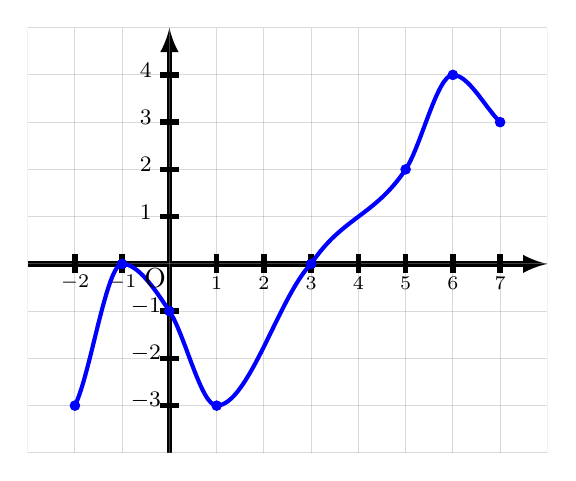
\begin{tikzpicture}[baseline,scale = 0.6]

    \tikzset{
      point/.style={
        thick,
        draw,
        cross out,
        inner sep=0pt,
        minimum width=5pt,
        minimum height=5pt,
      },
    }
    \clip (-3,-4) rectangle (8,5);
    	\draw[color ={black},line width = 2,>=latex,->] (-3,0)--(8,0);
	\draw[color ={black},line width = 2,>=latex,->] (0,-4)--(0,5);
	\draw[color ={gray},opacity = 0.3] (-3,0)--(8,0);
	\draw[color ={gray},opacity = 0.3] (-3,1)--(8,1);
	\draw[color ={gray},opacity = 0.3] (-3,2)--(8,2);
	\draw[color ={gray},opacity = 0.3] (-3,3)--(8,3);
	\draw[color ={gray},opacity = 0.3] (-3,4)--(8,4);
	\draw[color ={gray},opacity = 0.3] (-3,5)--(8,5);
	\draw[color ={gray},opacity = 0.3] (-3,0)--(8,0);
	\draw[color ={gray},opacity = 0.3] (-3,-1)--(8,-1);
	\draw[color ={gray},opacity = 0.3] (-3,-2)--(8,-2);
	\draw[color ={gray},opacity = 0.3] (-3,-3)--(8,-3);
	\draw[color ={gray},opacity = 0.3] (-3,-4)--(8,-4);
	\draw[color ={gray},opacity = 0.3] (0,-4)--(0,5);
	\draw[color ={gray},opacity = 0.3] (1,-4)--(1,5);
	\draw[color ={gray},opacity = 0.3] (2,-4)--(2,5);
	\draw[color ={gray},opacity = 0.3] (3,-4)--(3,5);
	\draw[color ={gray},opacity = 0.3] (4,-4)--(4,5);
	\draw[color ={gray},opacity = 0.3] (5,-4)--(5,5);
	\draw[color ={gray},opacity = 0.3] (6,-4)--(6,5);
	\draw[color ={gray},opacity = 0.3] (7,-4)--(7,5);
	\draw[color ={gray},opacity = 0.3] (8,-4)--(8,5);
	\draw[color ={gray},opacity = 0.3] (0,-4)--(0,5);
	\draw[color ={gray},opacity = 0.3] (-1,-4)--(-1,5);
	\draw[color ={gray},opacity = 0.3] (-2,-4)--(-2,5);
	\draw[color ={gray},opacity = 0.3] (-3,-4)--(-3,5);
	\draw[color ={black},line width = 2] (1,-0.2)--(1,0.2);
	\draw[color ={black},line width = 2] (2,-0.2)--(2,0.2);
	\draw[color ={black},line width = 2] (3,-0.2)--(3,0.2);
	\draw[color ={black},line width = 2] (4,-0.2)--(4,0.2);
	\draw[color ={black},line width = 2] (5,-0.2)--(5,0.2);
	\draw[color ={black},line width = 2] (6,-0.2)--(6,0.2);
	\draw[color ={black},line width = 2] (7,-0.2)--(7,0.2);
	\draw[color ={black},line width = 2] (-1,-0.2)--(-1,0.2);
	\draw[color ={black},line width = 2] (-2,-0.2)--(-2,0.2);
	\draw[color ={black},line width = 2] (-0.2,1)--(0.2,1);
	\draw[color ={black},line width = 2] (-0.2,2)--(0.2,2);
	\draw[color ={black},line width = 2] (-0.2,3)--(0.2,3);
	\draw[color ={black},line width = 2] (-0.2,4)--(0.2,4);
	\draw[color ={black},line width = 2] (-0.2,-1)--(0.2,-1);
	\draw[color ={black},line width = 2] (-0.2,-2)--(0.2,-2);
	\draw[color ={black},line width = 2] (-0.2,-3)--(0.2,-3);
	\draw (1,-0.4) node[anchor = center] {\scriptsize \color{black}{$1$}};
	\draw (2,-0.4) node[anchor = center] {\scriptsize \color{black}{$2$}};
	\draw (3,-0.4) node[anchor = center] {\scriptsize \color{black}{$3$}};
	\draw (4,-0.4) node[anchor = center] {\scriptsize \color{black}{$4$}};
	\draw (5,-0.4) node[anchor = center] {\scriptsize \color{black}{$5$}};
	\draw (6,-0.4) node[anchor = center] {\scriptsize \color{black}{$6$}};
	\draw (7,-0.4) node[anchor = center] {\scriptsize \color{black}{$7$}};
	\draw (-1,-0.4) node[anchor = center] {\scriptsize \color{black}{$-1$}};
	\draw (-2,-0.4) node[anchor = center] {\scriptsize \color{black}{$-2$}};
	\draw (-0.5,1.1) node[anchor = center] {\footnotesize \color{black}{$1$}};
	\draw (-0.5,2.1) node[anchor = center] {\footnotesize \color{black}{$2$}};
	\draw (-0.5,3.1) node[anchor = center] {\footnotesize \color{black}{$3$}};
	\draw (-0.5,4.1) node[anchor = center] {\footnotesize \color{black}{$4$}};
	\draw (-0.5,-0.9) node[anchor = center] {\footnotesize \color{black}{$-1$}};
	\draw (-0.5,-1.9) node[anchor = center] {\footnotesize \color{black}{$-2$}};
	\draw (-0.5,-2.9) node[anchor = center] {\footnotesize \color{black}{$-3$}};
	
	\draw[color = {blue},line width = 1.5, opacity = 1](-2,-3) .. controls +(0.33,0.67) and +(-0.33,0.00)  .. (-1.00,0.00)
 .. controls +(0.33,0.00) and +(-0.33,0.50)  .. (0.00,-1.00)
 .. controls +(0.33,-0.50) and +(-0.33,0.00)  .. (1.00,-3.00)
 .. controls +(0.67,0.00) and +(-0.67,-0.67)  .. (3.00,0.00)
 .. controls +(0.67,1.00) and +(-0.67,-1.00)  .. (5.00,2.00)
 .. controls +(0.33,0.50) and +(-0.33,0.00)  .. (6.00,4.00)
 .. controls +(0.33,0.00) and +(-0.33,0.33)  .. (7.00,3.00)
;

	 \filldraw[color={blue},fill={{blue}}] (-2,-3) circle (0.1);
	 \filldraw[color={blue},fill={{blue}}] (-1,0) circle (0.1);
	 \filldraw[color={blue},fill={{blue}}] (0,-1) circle (0.1);
	 \filldraw[color={blue},fill={{blue}}] (1,-3) circle (0.1);
	 \filldraw[color={blue},fill={{blue}}] (3,0) circle (0.1);
	 \filldraw[color={blue},fill={{blue}}] (5,2) circle (0.1);
	 \filldraw[color={blue},fill={{blue}}] (6,4) circle (0.1);
	 \filldraw[color={blue},fill={{blue}}] (7,3) circle (0.1);
	\draw [color={black}] (-0.3,-0.3) node[anchor = center,scale=1, rotate = 0] {O};

\end{tikzpicture} \end{minipage}
\end{enumerate}
\end{multicols}
\end{exercice}

\end{document}
\begin{enumerate}[itemsep=1em]
	\item Soit $u$ la fonction définie sur $\mathbb{R}$ par :\\          $u(x)=-x^2+4x+7$. \\          Quelles sont les coordonnées du sommet de la parabole représentant $u$ ?
	\item Soit $g$ la fonction définie sur $\mathbb{R}$ par :\\          $g(x)=3x^2+5$. \\          Quelles sont les coordonnées du sommet de la parabole représentant $g$ ?
	\item Soit $h$ la fonction définie sur $\mathbb{R}$ par :\\      $h(x)=-3x^2+4x+6$. \\
      Quelle est l'abscisse du sommet de la parabole représentant $h$ ?
	\item Soit $h$ la fonction définie sur $\mathbb{R}$ par :\\          $h(x)=-2x^2+8x+1$. \\          Quelles sont les coordonnées du sommet de la parabole représentant $h$ ?
	\item Soit $g$ la fonction définie sur $\mathbb{R}$ par :\\          $g(x)=3x^2+6x-2$. \\          Quelles sont les coordonnées du sommet de la parabole représentant $g$ ?
	\item Soit $v$ la fonction définie sur $\mathbb{R}$ par :\\          $v(x)=x^2-4x-3$. \\          Quelles sont les coordonnées du sommet de la parabole représentant $v$ ?
	\item Soit $h$ la fonction définie sur $\mathbb{R}$ par :\\          $h(x)=-3x^2-6x-7$. \\          Quelles sont les coordonnées du sommet de la parabole représentant $h$ ?
\end{enumerate}

%%% Local Variables:
%%% mode: LaTeX
%%% TeX-master: "../11.FA-01-S04-Evaluation-fonction"
%%% End:
\begin{multicols}{2}
\begin{enumerate}[itemsep=1em]
	\item \begin{minipage}[t]{\linewidth} Soit $r$ la fonction définie  par :\\
              $r(x)=3x^3-3x^2-5x$. \\
              $r$ est une fonction polynôme du second degré.	$\square\;$ Vrai\qquad $\square\;$ Faux\qquad  \end{minipage}
	\item \begin{minipage}[t]{\linewidth} Soit $w$ la fonction définie  par :\\
            $w(x)=-2x^2+4$. \\
            $w$ est une fonction polynôme du second degré.	$\square\;$ Vrai\qquad $\square\;$ Faux\qquad  \end{minipage}
	\item \begin{minipage}[t]{\linewidth} Soit $v$ la fonction définie  par :\\
              $v(x)=-7-9x^3$. \\
              $v$ est une fonction polynôme du second degré.	$\square\;$ Vrai\qquad $\square\;$ Faux\qquad  \end{minipage}
	\item \begin{minipage}[t]{\linewidth} Soit $h$ la fonction définie  par :\\
              $h(x)=-4+5x^3$. \\
              $h$ est une fonction polynôme du second degré.	$\square\;$ Vrai\qquad $\square\;$ Faux\qquad  \end{minipage}
	\item \begin{minipage}[t]{\linewidth} Soit $u$ la fonction définie  par :\\
                  $u(x)=4(x-6)^2$. \\
                  $u$ est une fonction polynôme du second degré.	$\square\;$ Vrai\qquad $\square\;$ Faux\qquad  \end{minipage}
	\item \begin{minipage}[t]{\linewidth} Soit $r$ la fonction définie  par :\\
            $r(x)=3x^2-2$. \\
            $r$ est une fonction polynôme du second degré.	$\square\;$ Vrai\qquad $\square\;$ Faux\qquad  \end{minipage}
	\item \begin{minipage}[t]{\linewidth} Soit $w$ la fonction définie  par :\\
            $w(x)=-6x-x^2-6$. \\
            $w$ est une fonction polynôme du second degré.	$\square\;$ Vrai\qquad $\square\;$ Faux\qquad  \end{minipage}
	\item \begin{minipage}[t]{\linewidth} Soit $u$ la fonction définie  par :\\
            $u(x)=5x+9-3x^2$. \\
            $u$ est une fonction polynôme du second degré.	$\square\;$ Vrai\qquad $\square\;$ Faux\qquad  \end{minipage}
	\item \begin{minipage}[t]{\linewidth} Soit $w$ la fonction définie  par :\\
                    $w(x)=-3x(x-3)(x+5)$. \\          
                    $w$ est une fonction polynôme du second degré.	$\square\;$ Vrai\qquad $\square\;$ Faux\qquad  \end{minipage}
	\item \begin{minipage}[t]{\linewidth} Soit $u$ la fonction définie  par :\\
                  $u(x)=2(x+7)^2-9$. \\         
                  $u$ est une fonction polynôme du second degré.	$\square\;$ Vrai\qquad $\square\;$ Faux\qquad  \end{minipage}
\end{enumerate}
\end{multicols}
\begin{multicols}{2}
\begin{enumerate}[itemsep=1.5em]
	\item \begin{minipage}[t]{\linewidth} Soit $f$ la fonction qui
            à $x$ associe $6x^2+4x$. \\ Quelle est l'image de $2$ ?\\
            \dtf \end{minipage}
	\item \begin{minipage}[t]{\linewidth} Soit $f: x \longmapsto 5x^2+2x-7$. \\ Quelle est l'image de $7$ ?\\ \dtf \end{minipage}
	\item \begin{minipage}[t]{\linewidth} Soit $f: x \longmapsto x^2+6x+5$. \\ Quelle est l'image de $6$ ?\\ \dtf \end{minipage}
	\item \begin{minipage}[t]{\linewidth} Soit $f(x)=x^2-2x+5$. \\ Quelle est l'image de $-3$ ?\\ \dtf \end{minipage}
	\item \begin{minipage}[t]{\linewidth} Soit $f: x \longmapsto x^2+5x+2$. \\ Quelle est l'image de $-9$ ?\\ \dtf \end{minipage}
	\item \begin{minipage}[t]{\linewidth} Soit $f: x \longmapsto x^2+4x+5$. \\ Quelle est l'image de $-2$ ?\\ \dtf \end{minipage}
	\item \begin{minipage}[t]{\linewidth} Soit $f$ la fonction qui à $x$ associe $3x^2+2x$. \\ Quelle est l'image de $5$ ?\\ \dtf \end{minipage}
	\item \begin{minipage}[t]{\linewidth} Soit $f(x)=x^2-3x+2$. \\ Quelle est l'image de $4$ ?\\ \dtf \end{minipage}
	\item \begin{minipage}[t]{\linewidth} Soit $f$ la fonction qui à $x$ associe $3x^2+4x$. \\ Quelle est l'image de $-2$ ?\\ \dtf \end{minipage}
	\item \begin{minipage}[t]{\linewidth} Soit $f(x)=3x^2-5x-2$. \\ Quelle est l'image de $-7$ ?\\ \dtf \end{minipage}
\end{enumerate}
\end{multicols}



%%% Local Variables:
%%% mode: LaTeX
%%% TeX-master: "../11.FA-01-S04-Evaluation-fonction"
%%% End:
\begin{multicols}{2}
\begin{enumerate}[itemsep=1.5em]
	\item \begin{minipage}[t]{\linewidth} Soit $f: x \longmapsto
            6x+4$. \\ Quelle est l'image de $2$ ?\\ \dtf \end{minipage}
	\item \begin{minipage}[t]{\linewidth} Soit $f: x \longmapsto 5x+2$. \\ Quelle est l'image de $2$ ?\\ \dtf \end{minipage}
	\item \begin{minipage}[t]{\linewidth} Soit $f: x \longmapsto 5x+2$. \\ Quelle est l'image de $4$ ?\\ \dtf \end{minipage}
	\item \begin{minipage}[t]{\linewidth} Soit $f: x \longmapsto 6x+4$. \\ Quelle est l'image de $6$ ?\\ \dtf \end{minipage}
	\item \begin{minipage}[t]{\linewidth} Soit $f: x \longmapsto 3x+2$. \\ Quelle est l'image de $5$ ?\\ \dtf \end{minipage}
	\item \begin{minipage}[t]{\linewidth} Soit $f: x \longmapsto 5x+2$. \\ Quelle est l'image de $-9$ ?\\ \dtf \end{minipage}
	\item \begin{minipage}[t]{\linewidth} Soit $f: x \longmapsto 6x+5$. \\ Quelle est l'image de $-9$ ?\\ \dtf \end{minipage}
	\item \begin{minipage}[t]{\linewidth} Soit $f: x \longmapsto 2x+5$. \\ Quelle est l'image de $-7$ ?\\ \dtf \end{minipage}
	\item \begin{minipage}[t]{\linewidth} Soit $f: x \longmapsto 5x+4$. \\ Quelle est l'image de $7$ ?\\ \dtf \end{minipage}
	\item \begin{minipage}[t]{\linewidth} Soit $f: x \longmapsto 3x+2$. \\ Quelle est l'image de $8$ ?\\ \dtf \end{minipage}
\end{enumerate}
\end{multicols}

%%% Local Variables:
%%% mode: LaTeX
%%% TeX-master: "../11.FA-01-S04-Evaluation-fonction"
%%% End:
%% Font size %%
\documentclass[11pt]{article}

%% Load the custom package
\usepackage{Mathdoc}

%% Numéro de séquence %% Titre de la séquence %%
\renewcommand{\centerhead}{Chap. 4 : Fonctions polynôme de degré 2}

%% Spacing commands %%
\renewcommand{\baselinestretch}{1}
\setlength{\parindent}{0pt}

\begin{document}

\section{Fonctions affines}

\begin{exercice}[0][Exercice corrig�.]
\textbf{Soit $f: x \longmapsto 6x+4$. \\ Quelle est l'image de $1$ ?}
\\
Correction :\\
\textit{On remplace $x$ par $1$ dans l'expression de $f(x)$ : \\
$f(1)=6 \times 1 + 4$ \\
$f(1)=10$}
\end{exercice}

\begin{exercice}[1][Calculs d'images.]
\begin{multicols}{2}
\begin{enumerate}[itemsep=1.5em]
	\item \begin{minipage}[t]{\linewidth} Soit $f: x \longmapsto
            6x+4$. \\ Quelle est l'image de $2$ ?\\ \dtf \end{minipage}
	\item \begin{minipage}[t]{\linewidth} Soit $f: x \longmapsto 5x+2$. \\ Quelle est l'image de $2$ ?\\ \dtf \end{minipage}
	\item \begin{minipage}[t]{\linewidth} Soit $f: x \longmapsto 5x+2$. \\ Quelle est l'image de $4$ ?\\ \dtf \end{minipage}
	\item \begin{minipage}[t]{\linewidth} Soit $f: x \longmapsto 6x+4$. \\ Quelle est l'image de $6$ ?\\ \dtf \end{minipage}
	\item \begin{minipage}[t]{\linewidth} Soit $f: x \longmapsto 3x+2$. \\ Quelle est l'image de $5$ ?\\ \dtf \end{minipage}
	\item \begin{minipage}[t]{\linewidth} Soit $f: x \longmapsto 5x+2$. \\ Quelle est l'image de $-9$ ?\\ \dtf \end{minipage}
	\item \begin{minipage}[t]{\linewidth} Soit $f: x \longmapsto 6x+5$. \\ Quelle est l'image de $-9$ ?\\ \dtf \end{minipage}
	\item \begin{minipage}[t]{\linewidth} Soit $f: x \longmapsto 2x+5$. \\ Quelle est l'image de $-7$ ?\\ \dtf \end{minipage}
	\item \begin{minipage}[t]{\linewidth} Soit $f: x \longmapsto 5x+4$. \\ Quelle est l'image de $7$ ?\\ \dtf \end{minipage}
	\item \begin{minipage}[t]{\linewidth} Soit $f: x \longmapsto 3x+2$. \\ Quelle est l'image de $8$ ?\\ \dtf \end{minipage}
\end{enumerate}
\end{multicols}

%%% Local Variables:
%%% mode: LaTeX
%%% TeX-master: "../11.FA-01-S04-Evaluation-fonction"
%%% End:

\end{exercice}

\begin{exercice}[2][Calculs d'images.]
  \begin{enumerate}
    \begin{multicols}{2}
    \item \item Soit $f$ la fonction définie par $f(x)=\dfrac{5}{2}x-6$. \\
      Quelle est l'image de $14$ ?\\ \dtf
    \item Soit $f$ la fonction définie par $f(x)=\dfrac{5}{4}x-9$. \\
      Quelle est l'image de $28$ ?\\ \dtf
    \item Soit $f$ la fonction définie par $f(x)=\dfrac{3}{5}x+3$. \\
      Quelle est l'image de $20$ ?\\ \dtf
    \item Soit $f$ la fonction définie par $f(x)=\dfrac{2}{5}x+1$. \\
      Quelle est l'image de $10$ ?\\ \dtf
    \end{multicols}
  \end{enumerate}
\end{exercice}
\newpage
\section{Polynômes du second degré}

\begin{exercice}[0][Exercice corrigé.]
\textbf{Soit $f(x)=6x^2+4x-3$. \\ Quelle est l'image de $1$ ?}
\\
Correction :\\
\textit{On remplace $x$ par $1$ dans l'expression de $f(x)$ : \\
$f(1)=6 \times 1^2 + 4 \times 1 - 3$ \\
$f(1)=6+4-3$ \\
$f(1)=7$ }
\end{exercice}

\begin{exercice}[1][Calculs d'images.]
\begin{multicols}{2}
\begin{enumerate}[itemsep=1.5em]
	\item \begin{minipage}[t]{\linewidth} Soit $f$ la fonction qui
            à $x$ associe $6x^2+4x$. \\ Quelle est l'image de $2$ ?\\
            \dtf \end{minipage}
	\item \begin{minipage}[t]{\linewidth} Soit $f: x \longmapsto 5x^2+2x-7$. \\ Quelle est l'image de $7$ ?\\ \dtf \end{minipage}
	\item \begin{minipage}[t]{\linewidth} Soit $f: x \longmapsto x^2+6x+5$. \\ Quelle est l'image de $6$ ?\\ \dtf \end{minipage}
	\item \begin{minipage}[t]{\linewidth} Soit $f(x)=x^2-2x+5$. \\ Quelle est l'image de $-3$ ?\\ \dtf \end{minipage}
	\item \begin{minipage}[t]{\linewidth} Soit $f: x \longmapsto x^2+5x+2$. \\ Quelle est l'image de $-9$ ?\\ \dtf \end{minipage}
	\item \begin{minipage}[t]{\linewidth} Soit $f: x \longmapsto x^2+4x+5$. \\ Quelle est l'image de $-2$ ?\\ \dtf \end{minipage}
	\item \begin{minipage}[t]{\linewidth} Soit $f$ la fonction qui à $x$ associe $3x^2+2x$. \\ Quelle est l'image de $5$ ?\\ \dtf \end{minipage}
	\item \begin{minipage}[t]{\linewidth} Soit $f(x)=x^2-3x+2$. \\ Quelle est l'image de $4$ ?\\ \dtf \end{minipage}
	\item \begin{minipage}[t]{\linewidth} Soit $f$ la fonction qui à $x$ associe $3x^2+4x$. \\ Quelle est l'image de $-2$ ?\\ \dtf \end{minipage}
	\item \begin{minipage}[t]{\linewidth} Soit $f(x)=3x^2-5x-2$. \\ Quelle est l'image de $-7$ ?\\ \dtf \end{minipage}
\end{enumerate}
\end{multicols}



%%% Local Variables:
%%% mode: LaTeX
%%% TeX-master: "../11.FA-01-S04-Evaluation-fonction"
%%% End:

\end{exercice}

\begin{exercice}[2][Calculs d'images.]
  \begin{multicols}{2}
    \begin{enumerate}[itemsep=1.5em]
    \item Soit $f$ telle que $f(x)=\dfrac{-2x^2+2x}{x^2-2x}$. \\
      Quelle est l'image de $4$ ?\\ \dtf
    \item Soit $f$ telle que $f(x)=\dfrac{13x^2+4x}{x^2+13x}$. \\
      Quelle est l'image de $-9$ ?\\ \dtf
    \item Soit $f$ la fonction qui à $x$ associe $\dfrac{x}{x-3}$. \\
      Quelle est l'image de $5$ ?\\ \dtf
    \item Soit $f: x \longmapsto \dfrac{x-9}{x^2-18x+81}$. \\
      Quelle est l'image de $-5$ ?\\ \dtf
    \end{enumerate}
  \end{multicols}
\end{exercice}

\section{Reconnaitre un polynôme du second degré}
\begin{exercice}[1][Reconnaitre un polynôme.]
\begin{multicols}{2}
\begin{enumerate}[itemsep=1em]
	\item \begin{minipage}[t]{\linewidth} Soit $r$ la fonction définie  par :\\
              $r(x)=3x^3-3x^2-5x$. \\
              $r$ est une fonction polynôme du second degré.	$\square\;$ Vrai\qquad $\square\;$ Faux\qquad  \end{minipage}
	\item \begin{minipage}[t]{\linewidth} Soit $w$ la fonction définie  par :\\
            $w(x)=-2x^2+4$. \\
            $w$ est une fonction polynôme du second degré.	$\square\;$ Vrai\qquad $\square\;$ Faux\qquad  \end{minipage}
	\item \begin{minipage}[t]{\linewidth} Soit $v$ la fonction définie  par :\\
              $v(x)=-7-9x^3$. \\
              $v$ est une fonction polynôme du second degré.	$\square\;$ Vrai\qquad $\square\;$ Faux\qquad  \end{minipage}
	\item \begin{minipage}[t]{\linewidth} Soit $h$ la fonction définie  par :\\
              $h(x)=-4+5x^3$. \\
              $h$ est une fonction polynôme du second degré.	$\square\;$ Vrai\qquad $\square\;$ Faux\qquad  \end{minipage}
	\item \begin{minipage}[t]{\linewidth} Soit $u$ la fonction définie  par :\\
                  $u(x)=4(x-6)^2$. \\
                  $u$ est une fonction polynôme du second degré.	$\square\;$ Vrai\qquad $\square\;$ Faux\qquad  \end{minipage}
	\item \begin{minipage}[t]{\linewidth} Soit $r$ la fonction définie  par :\\
            $r(x)=3x^2-2$. \\
            $r$ est une fonction polynôme du second degré.	$\square\;$ Vrai\qquad $\square\;$ Faux\qquad  \end{minipage}
	\item \begin{minipage}[t]{\linewidth} Soit $w$ la fonction définie  par :\\
            $w(x)=-6x-x^2-6$. \\
            $w$ est une fonction polynôme du second degré.	$\square\;$ Vrai\qquad $\square\;$ Faux\qquad  \end{minipage}
	\item \begin{minipage}[t]{\linewidth} Soit $u$ la fonction définie  par :\\
            $u(x)=5x+9-3x^2$. \\
            $u$ est une fonction polynôme du second degré.	$\square\;$ Vrai\qquad $\square\;$ Faux\qquad  \end{minipage}
	\item \begin{minipage}[t]{\linewidth} Soit $w$ la fonction définie  par :\\
                    $w(x)=-3x(x-3)(x+5)$. \\          
                    $w$ est une fonction polynôme du second degré.	$\square\;$ Vrai\qquad $\square\;$ Faux\qquad  \end{minipage}
	\item \begin{minipage}[t]{\linewidth} Soit $u$ la fonction définie  par :\\
                  $u(x)=2(x+7)^2-9$. \\         
                  $u$ est une fonction polynôme du second degré.	$\square\;$ Vrai\qquad $\square\;$ Faux\qquad  \end{minipage}
\end{enumerate}
\end{multicols}

\end{exercice}

\section{Identifier les coefficients}

\begin{exercice}[0][Exercice Corrigé.]
Identifier les valeurs de $a$, $b$ et
$c$.
\begin{enumerate}[itemsep=1em,label={}]
\item $A(x) = 2x^2+3x+4$. \\ \\
\textit{$A(x)$ est une fonction polynôme du second degré écrite sous forme
développée $ax^2+bx+c$, \\avec : \\}
$a = 2$ \\ 
$b = 3$ \\ 
$c = 4$   
\end{enumerate}
\end{exercice}


\begin{exercice}[1][Identifier les coefficients.]
Dans chacun des cas suivant, identifier les valeurs de $a$, $b$ et
$c$.
\begin{enumerate}[itemsep=1em,label={}]
  \begin{multicols}{2}
  \item $A(x) = x^2+5x$. \\ a = \dotfill \\ b = \dotfill \\ c =
    \dotfill
  \item $B(x) = 4x^2+3x$. \\ a = \dotfill \\ b = \dotfill \\ c =
    \dotfill
  \item $C(x) = x^2+3$. \\ a = \dotfill \\ b = \dotfill \\ c =
    \dotfill
  \item $D(x) = 3x^2+2x+5$. \\ a = \dotfill \\ b = \dotfill \\ c =
    \dotfill
  \item $E(x) = 3x^2+2x+2$. \\ a = \dotfill \\ b = \dotfill \\ c =
    \dotfill
  \item $F(x) = 2x+2-7x^2$. \\ a = \dotfill \\ b = \dotfill \\ c =
    \dotfill
  \end{multicols}
\end{enumerate}
\end{exercice}


\begin{exercice}[2][Identifier les coefficients.]
Dans chacun des cas suivant, identifier les valeurs de $a$, $b$ et
$c$.
\begin{enumerate}[itemsep=1em,label={}]
  \begin{multicols}{2}
        \item $A(x) = 4x^2-4x+2$. \\ a = \dotfill \\ b = \dotfill \\ c =
    \dotfill
	\item $B(x) = x^2-5x-4$. \\ a = \dotfill \\ b = \dotfill \\ c =
    \dotfill
	\item $C(x) = 2x-5x^2$. \\ a = \dotfill \\ b = \dotfill \\ c =
    \dotfill
	\item $D(x) = -x-1+5x^2$. \\ a = \dotfill \\ b = \dotfill \\ c =
    \dotfill
	\item $E(x) = -5-2x^2-3x$. \\ a = \dotfill \\ b = \dotfill \\ c =
    \dotfill
	\item $F(x) = -5x^2-2-x$. \\ a = \dotfill \\ b = \dotfill \\ c =
    \dotfill
  \end{multicols}
\end{enumerate}
\end{exercice}


\begin{exercice}[3][Identifier les coefficients.]
Dans chacun des cas suivant, identifier les valeurs de $a$, $b$ et
$c$.
\begin{enumerate}[itemsep=1em,label={}]
  \begin{multicols}{2}
        \item $A(x) = -4x-2x^2$. \\ a = \dotfill \\ b = \dotfill \\ c =
    \dotfill
	\item $B(x) = -153x^2-\frac{3}{4}$. \\ a = \dotfill \\ b = \dotfill \\ c =
    \dotfill
  \end{multicols}
\end{enumerate}
\end{exercice}

\newpage

\section{Coordonnées du sommet}

\begin{exercice}[0][Exercice Corrigé.]
 Soit $u$ la fonction définie sur $\mathbb{R}$ par :\\
 $u(x)=-x^2+4x+7$. \\
Quelles sont les coordonnées du sommet de la parabole représentant $u$ ? \\
Correction :\\
\textit{ $u$ est une fonction polynôme du second degré écrite sous
forme développée $ax^2+bx+c$.\\
Avec $a=-1$ ; $b=+4$ ; $c=+7$. \\
          Le sommet de la parabole a pour abscisse $\alpha =-\dfrac{b}{2a}$.\\
          $\alpha =-\dfrac{4}{2\times(-1) }= 2$ \\
          L'ordonnée du sommet est donnée par $f(\alpha)$, soit \\
          $f(2)=-1\times 2^2+4\times 2+7=11$.}
\end{exercice}


\begin{exercice}[3][Sur le cahiers, déterminer les coordonnées du sommet.]
\begin{enumerate}[itemsep=1em]
	\item Soit $u$ la fonction définie sur $\mathbb{R}$ par :\\          $u(x)=-x^2+4x+7$. \\          Quelles sont les coordonnées du sommet de la parabole représentant $u$ ?
	\item Soit $g$ la fonction définie sur $\mathbb{R}$ par :\\          $g(x)=3x^2+5$. \\          Quelles sont les coordonnées du sommet de la parabole représentant $g$ ?
	\item Soit $h$ la fonction définie sur $\mathbb{R}$ par :\\      $h(x)=-3x^2+4x+6$. \\
      Quelle est l'abscisse du sommet de la parabole représentant $h$ ?
	\item Soit $h$ la fonction définie sur $\mathbb{R}$ par :\\          $h(x)=-2x^2+8x+1$. \\          Quelles sont les coordonnées du sommet de la parabole représentant $h$ ?
	\item Soit $g$ la fonction définie sur $\mathbb{R}$ par :\\          $g(x)=3x^2+6x-2$. \\          Quelles sont les coordonnées du sommet de la parabole représentant $g$ ?
	\item Soit $v$ la fonction définie sur $\mathbb{R}$ par :\\          $v(x)=x^2-4x-3$. \\          Quelles sont les coordonnées du sommet de la parabole représentant $v$ ?
	\item Soit $h$ la fonction définie sur $\mathbb{R}$ par :\\          $h(x)=-3x^2-6x-7$. \\          Quelles sont les coordonnées du sommet de la parabole représentant $h$ ?
\end{enumerate}

%%% Local Variables:
%%% mode: LaTeX
%%% TeX-master: "../11.FA-01-S04-Evaluation-fonction"
%%% End:

\end{exercice}


\end{document}
%% Font size %%
\documentclass[11pt]{article}

%% Load the custom package
\usepackage{Mathdoc}

%% Numéro de séquence %% Titre de la séquence %%
\renewcommand{\centerhead}{Chap. 3 : Identitifer les angles particuliers}

%% Spacing commands %%
\renewcommand{\baselinestretch}{1}
\setlength{\parindent}{0pt}

\begin{document}

\section{Identifier les angles particuliers}


\begin{exemple}
  \begin{multicols}{2}
    \begin{center}
      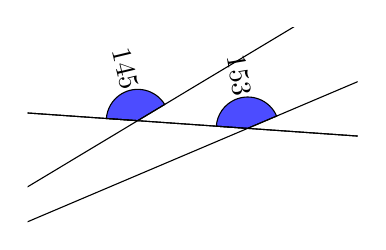
\begin{tikzpicture}[baseline,scale = 0.4,rotate=90]

    
        \tikzset{ point/.style={ thick, draw, cross out, inner
        sep=0pt, minimum width=5pt, minimum height=5pt, }, } \clip
        (-3.081320233229482,-4.989038226169209) rectangle
        (3.0925418121643005,5.487820251299121); \draw
        [color={black},preaction={fill,color = {blue},opacity = 0.7}]
        (0.20926942123237668,2.992692150779472) --
        (0.1395129474882511,1.9951281005196482) --
        (0.6545510223983052,1.1379607998175363) arc (-58.68:86.32:1) ;
        \draw[color={black}]
        (-25.612390798014463,44.85349313562526)--(26.406454767901018,-41.72040423528807);
        \draw[color={black}]
        (-3.348310739718021,-47.88307441247155)--(3.6970931084386485,52.87089466377067);
        \draw [color={black},preaction={fill,color = {blue},opacity =
        0.7}] (-0.034878236872062596,-0.4987820251299113) --
        (-0.10463471061618815,-1.496346075389736) --
        (0.2860964178730856,-2.4168509288421767) arc (-66.73:86.27:1)
        ; \draw[color={black}]
        (-19.641191135079886,44.52889659723229)--(19.822652842336783,-48.44209360146421);
        \draw[color={black}]
        (-3.5924583978224613,-51.37454858838095)--(3.45294545033421,49.379420487861296);
        \draw [color={black}] (1.79,2.39) node[anchor =
        center,scale=1, rotate = -76.50006] {\ang{145}}; \draw
        [color={black}] (1.57,-1.22) node[anchor = center,scale=1,
        rotate = -80.50002] {\ang{153}};

      \end{tikzpicture}
    \end{center}

    Ci-dessus les deux angles sont correspondants.

    \begin{center}
      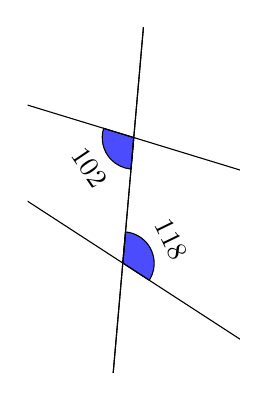
\begin{tikzpicture}[baseline,scale = 0.4,rotate=180]


    \tikzset{
      point/.style={
        thick,
        draw,
        cross out,
        inner sep=0pt,
        minimum width=5pt,
        minimum height=5pt,
      },
    }
    \clip (-3.543225753384422,-5.480973490458728) rectangle (3.1946027823937895,5.480973490458728);
    	\draw  [color={black},preaction={fill,color = {blue},opacity = 0.7}] (0.08715574274765758,0.9961946980917454) -- (0.17431148549531622,1.9923893961834909) -- (-0.6643590824501077,2.537028431198518) arc (147.48:265.48:1) ;
	\draw[color={black}] (-41.75921691177589,29.22434114693484)--(42.94651045071194,-25.784201389582886);
	\draw[color={black}] (-4.183475651887591,-47.8173455084038)--(4.619254365625881,52.79831899886253);
	\draw  [color={black},preaction={fill,color = {blue},opacity = 0.7}] (-0.08715574274765814,-0.9961946980917457) -- (-0.17431148549531658,-1.992389396183491) -- (0.7819932704677189,-2.284761100906228) arc (-17.25:84.75:1) ;
	\draw[color={black}] (-47.98954928364709,12.626195839953347)--(48.597231068619486,-16.903346337043065);
	\draw[color={black}] (-4.532098622878223,-51.80212430077077)--(4.270631394635249,48.81354020649553);
	\draw [color={black}] (-1.35,1.25) node[anchor = center,scale=1, rotate = -64.00014] {\ang{118}};
	\draw [color={black}] (1.24,-1.04) node[anchor = center,scale=1, rotate = -55.999719999999996] {\ang{102}};

      \end{tikzpicture}
    \end{center}

    Ci-dessus les deux angles sont alternes-internes.

\end{multicols}
  \end{exemple}


\begin{exercice}[1]
\textbf{Les angles marqués sont-ils alternes-internes, correspondants ou ni l'un, ni l'autre ?}
\begin{multicols}{3}
\begin{enumerate}
	\item \begin{minipage}[t]{\linewidth} 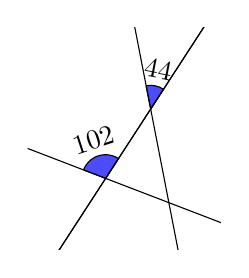
\begin{tikzpicture}[baseline,scale = 0.3]

    \tikzset{
      point/.style={
        thick,
        draw,
        cross out,
        inner sep=0pt,
        minimum width=5pt,
        minimum height=5pt,
      },
    }
    \clip (-4.390019349521659,-4.69335283972712) rectangle (3.78572476438357,4.702887402261128);
    	\draw  [color={black},preaction={fill,color = {blue},opacity = 0.7}] (0.626149557145996,2.2396330353657996) -- (0.8169585525225405,1.2580058519181354) -- (1.3615975875375679,2.0966764198635595) arc (56.72:100.72:1) ;
	\draw[color={black}] (-8.723491216304707,50.33936502430133)--(10.548217316726333,-48.804980503912724);
	\draw[color={black}] (-26.414993198228814,-40.67552254535305)--(28.59354933828892,44.030204817134745);
	\draw  [color={black},preaction={fill,color = {blue},opacity = 0.7}] (-2.0228584965272556,-1.3189731863455467) -- (-1.0892780700300544,-1.6773411358908479) -- (-0.5446390350150268,-0.8386705679454244) arc (56.72:158.72:1) ;
	\draw[color={black}] (-47.76829939489014,16.241056341374165)--(46.523323681327234,-19.954106562701163);
	\draw[color={black}] (-28.321229820781415,-43.610869533162045)--(26.687312715736333,41.094857829325775);
	\draw [color={black}] (1.14,2.93) node[anchor = center,scale=1, rotate = -10.995039999999989] {\ang{44}};
	\draw [color={black}] (-1.61,-0.06) node[anchor = center,scale=1, rotate = -341.99936] {\ang{102}};

\end{tikzpicture}\\ \end{minipage}
	\item \begin{minipage}[t]{\linewidth} 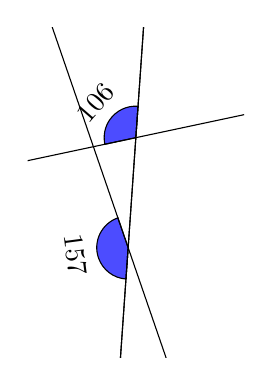
\begin{tikzpicture}[baseline,scale = 0.4]

    \tikzset{
      point/.style={
        thick,
        draw,
        cross out,
        inner sep=0pt,
        minimum width=5pt,
        minimum height=5pt,
      },
    }
    \clip (-3.329808091585229,-5.487820251299121) rectangle (3.539077512817605,4.989038226169209);
    	\draw  [color={black},preaction={fill,color = {blue},opacity = 0.7}] (-0.8735128901176171,1.2884343845719772) -- (0.1046347106161884,1.4963460753897364) -- (0.17439118436031364,2.4939101256495606) arc (85.69:191.69:1) ;
	\draw[color={black}] (-48.802745326074096,-8.899238465498234)--(49.99016234804028,12.099842307095466);
	\draw[color={black}] (-3.3831889765900853,-48.381856437601485)--(3.662214871566587,52.372112638640786);
	\draw  [color={black},preaction={fill,color = {blue},opacity = 0.7}] (-0.20926942123237727,-2.992692150779473) -- (-0.1395129474882513,-1.9951281005196484) -- (-0.4650811019454078,-1.0496095249203314) arc (109.17:266.17:1) ;
	\draw[color={black}] (-16.41792067034609,45.280800679446195)--(16.464462929826745,-50.21657545608481);
	\draw[color={black}] (-3.627336634694524,-51.87333061351086)--(3.4180672134621473,48.88063846273138);
	\draw [color={black}] (-1.18,2.61) node[anchor = center,scale=1, rotate = -311.0002] {\ang{106}};
	\draw [color={black}] (-1.82,-2.22) node[anchor = center,scale=1, rotate = -82.50011] {\ang{157}};

\end{tikzpicture}\\ \end{minipage}
	\item \begin{minipage}[t]{\linewidth} 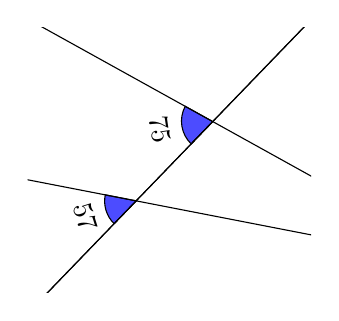
\begin{tikzpicture}[baseline,scale = 0.4]

    \tikzset{
      point/.style={
        thick,
        draw,
        cross out,
        inner sep=0pt,
        minimum width=5pt,
        minimum height=5pt,
      },
    }
    \clip (-4.486869106031488,-4.000328516779962) rectangle (4.5131758623361815,4.4200065683925605);
    	\draw  [color={black},preaction={fill,color = {blue},opacity = 0.7}] (0.6946583704589984,0.7193398003386509) -- (1.3893167409179954,1.4386796006773026) -- (0.5146970337785991,1.9234892209236392) arc (151.86:226.86:1) ;
	\draw[color={black}] (-42.34166861605179,25.679160612994153)--(45.99492180502718,-23.286611031885883);
	\draw[color={black}] (-33.343601782031854,-34.52831041625525)--(36.816893634326846,38.12500941794851);
	\draw  [color={black},preaction={fill,color = {blue},opacity = 0.7}] (-1.7366459261474938,-1.798349500846627) -- (-1.0419875556884963,-1.0790097005079757) -- (-2.0236147391361605,-0.8882007051314311) arc (168.54:225.54:1) ;
	\draw[color={black}] (-50.123346728071695,8.461440068319265)--(49.02099880014237,-10.810268464711761);
	\draw[color={black}] (-35.77490607863836,-37.04599971744053)--(34.38558933772037,35.60732011676323);
	\draw [color={black}] (-0.29,1.19) node[anchor = center,scale=1, rotate = -81.50019] {\ang{75}};
	\draw [color={black}] (-2.66,-1.59) node[anchor = center,scale=1, rotate = -72.49962] {\ang{57}};

\end{tikzpicture}\\ \end{minipage}
	\item \begin{minipage}[t]{\linewidth} 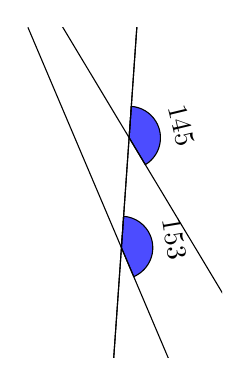
\begin{tikzpicture}[baseline,scale = 0.4]

    \tikzset{
      point/.style={
        thick,
        draw,
        cross out,
        inner sep=0pt,
        minimum width=5pt,
        minimum height=5pt,
      },
    }
    \clip (-3.081320233229482,-4.989038226169209) rectangle (3.0925418121643005,5.487820251299121);
    	\draw  [color={black},preaction={fill,color = {blue},opacity = 0.7}] (0.20926942123237668,2.992692150779472) -- (0.1395129474882511,1.9951281005196482) -- (0.6545510223983052,1.1379607998175363) arc (-58.68:86.32:1) ;
	\draw[color={black}] (-25.612390798014463,44.85349313562526)--(26.406454767901018,-41.72040423528807);
	\draw[color={black}] (-3.348310739718021,-47.88307441247155)--(3.6970931084386485,52.87089466377067);
	\draw  [color={black},preaction={fill,color = {blue},opacity = 0.7}] (-0.034878236872062596,-0.4987820251299113) -- (-0.10463471061618815,-1.496346075389736) -- (0.2860964178730856,-2.4168509288421767) arc (-66.73:86.27:1) ;
	\draw[color={black}] (-19.641191135079886,44.52889659723229)--(19.822652842336783,-48.44209360146421);
	\draw[color={black}] (-3.5924583978224613,-51.37454858838095)--(3.45294545033421,49.379420487861296);
	\draw [color={black}] (1.79,2.39) node[anchor = center,scale=1, rotate = -76.50006] {\ang{145}};
	\draw [color={black}] (1.57,-1.22) node[anchor = center,scale=1, rotate = -80.50002] {\ang{153}};

\end{tikzpicture}\\ \end{minipage}
	\item \begin{minipage}[t]{\linewidth} 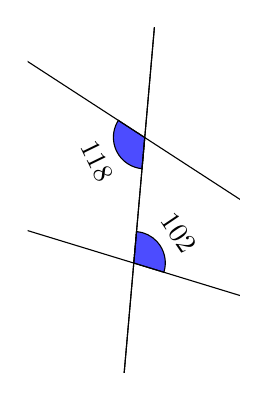
\begin{tikzpicture}[baseline,scale = 0.4]

    \tikzset{
      point/.style={
        thick,
        draw,
        cross out,
        inner sep=0pt,
        minimum width=5pt,
        minimum height=5pt,
      },
    }
    \clip (-3.543225753384422,-5.480973490458728) rectangle (3.1946027823937895,5.480973490458728);
    	\draw  [color={black},preaction={fill,color = {blue},opacity = 0.7}] (0.08715574274765758,0.9961946980917454) -- (0.17431148549531622,1.9923893961834909) -- (-0.6643590824501077,2.537028431198518) arc (147.48:265.48:1) ;
	\draw[color={black}] (-41.75921691177589,29.22434114693484)--(42.94651045071194,-25.784201389582886);
	\draw[color={black}] (-4.183475651887591,-47.8173455084038)--(4.619254365625881,52.79831899886253);
	\draw  [color={black},preaction={fill,color = {blue},opacity = 0.7}] (-0.08715574274765814,-0.9961946980917457) -- (-0.17431148549531658,-1.992389396183491) -- (0.7819932704677189,-2.284761100906228) arc (-17.25:84.75:1) ;
	\draw[color={black}] (-47.98954928364709,12.626195839953347)--(48.597231068619486,-16.903346337043065);
	\draw[color={black}] (-4.532098622878223,-51.80212430077077)--(4.270631394635249,48.81354020649553);
	\draw [color={black}] (-1.35,1.25) node[anchor = center,scale=1, rotate = -64.00014] {\ang{118}};
	\draw [color={black}] (1.24,-1.04) node[anchor = center,scale=1, rotate = -55.999719999999996] {\ang{102}};

\end{tikzpicture}\\ \end{minipage}
	\item \begin{minipage}[t]{\linewidth} 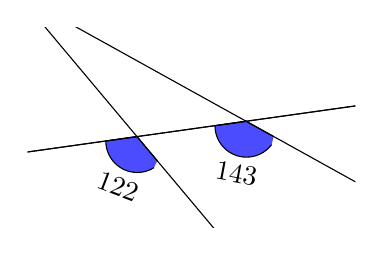
\begin{tikzpicture}[baseline,scale = 0.4]

    \tikzset{
      point/.style={
        thick,
        draw,
        cross out,
        inner sep=0pt,
        minimum width=5pt,
        minimum height=5pt,
      },
    }
    \clip (-4.956206309337067,-3.0958463764853414) rectangle (5.451340343707852,3.249879544778853);
    	\draw  [color={black},preaction={fill,color = {blue},opacity = 0.7}] (2.8551558446225362,-0.20646341832620585) -- (1.9805361374831405,0.27834620192013104) -- (0.9902680687415701,0.13917310096006552) arc (-180:-37:1) ;
	\draw[color={black}] (-41.75044921948663,24.518827214236982)--(46.58614120159231,-24.446944430643057);
	\draw[color={black}] (-47.53286729959539,-6.680308846083142)--(52.48420764330324,7.37617435088347);
	\draw  [color={black},preaction={fill,color = {blue},opacity = 0.7}] (-0.842614493425816,-0.9748040945590766) -- (-1.4854021031123552,-0.20875965144009823) -- (-2.475670171853926,-0.34793275240016364) arc (-180:-58:1) ;
	\draw[color={black}] (-33.62478258743933,38.09346250450881)--(31.296765990901154,-39.27702625050798);
	\draw[color={black}] (-50.99880554019087,-7.16741469944337)--(49.01826940270773,6.889068497523239);
	\draw [color={black}] (1.67,-1.39) node[anchor = center,scale=1, rotate = -10.49892] {\ang{143}};
	\draw [color={black}] (-2.09,-1.8) node[anchor = center,scale=1, rotate = -20.99966] {\ang{122}};

\end{tikzpicture}\\ \end{minipage}
	\item \begin{minipage}[t]{\linewidth} 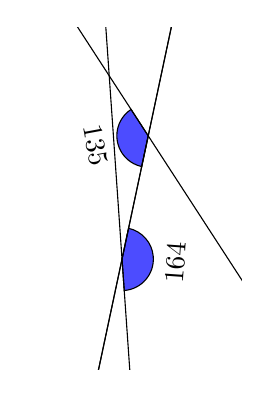
\begin{tikzpicture}[baseline,scale = 0.4]

    \tikzset{
      point/.style={
        thick,
        draw,
        cross out,
        inner sep=0pt,
        minimum width=5pt,
        minimum height=5pt,
      },
    }
    \clip (-3.4116822670772207,-5.448987352247084) rectangle (3.387356724494242,5.390738003669028);
    	\draw  [color={black},preaction={fill,color = {blue},opacity = 0.7}] (0.20791169081775973,0.9781476007338062) -- (0.4158233816355189,1.9562952014676114) -- (-0.12881565337950807,2.794965769413035) arc (123.28:258.28:1) ;
	\draw[color={black}] (-26.816128369115834,43.8898235987388)--(28.1924141674019,-40.815903763749);
	\draw[color={black}] (-9.979761159252451,-46.95108483522266)--(11.01931961334125,51.84182283889169);
	\draw  [color={black},preaction={fill,color = {blue},opacity = 0.7}] (-0.20791169081775984,-0.9781476007338058) -- (-0.4158233816355195,-1.9562952014676112) -- (-0.3460669078913941,-2.9538592517274354) arc (-85.69:78.31:1) ;
	\draw[color={black}] (-3.903647068841793,47.9219073115236)--(3.1417567793148793,-52.832061764718645);
	\draw[color={black}] (-10.811407922523491,-50.86367523815789)--(10.187672850070213,47.92923243595647);
	\draw [color={black}] (-1.26,1.65) node[anchor = center,scale=1, rotate = -79.4997] {\ang{135}};
	\draw [color={black}] (1.28,-2.07) node[anchor = center,scale=1, rotate = 85.99994] {\ang{164}};

\end{tikzpicture}\\ \end{minipage}
	\item \begin{minipage}[t]{\linewidth} 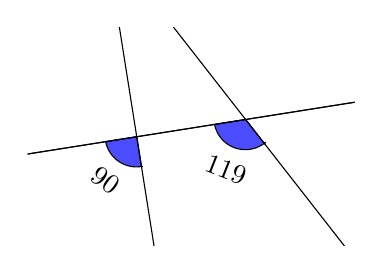
\begin{tikzpicture}[baseline,scale = 0.4]

    \tikzset{
      point/.style={
        thick,
        draw,
        cross out,
        inner sep=0pt,
        minimum width=5pt,
        minimum height=5pt,
      },
    }
    \clip (-4.94459753267812,-3.6977167193457596) rectangle (5.438441702975689,3.228413324225068);
    	\draw  [color={black},preaction={fill,color = {blue},opacity = 0.7}] (2.5910381565159337,-0.4751418235262608) -- (1.9753766811902758,0.3128689300804615) -- (0.9876883405951378,0.15643446504023095) arc (-168.54:-49.53999999999999:1) ;
	\draw[color={black}] (-28.807697085092634,39.71340661041656)--(33.374111922798846,-39.87567950386236);
	\draw[color={black}] (-47.40904034856661,-7.508854321931083)--(52.3474820515423,8.291026647132238);
	\draw  [color={black},preaction={fill,color = {blue},opacity = 0.7}] (-1.3250980458524761,-1.2223400381554839) -- (-1.4815325108927069,-0.234651697560346) -- (-2.4692208514878446,-0.3910861626005768) arc (-168.54:-78.53999999999999:1) ;
	\draw[color={black}] (-9.303255762904255,49.149765332196544)--(6.496625206159072,-50.606757067912376);
	\draw[color={black}] (-50.865949540649595,-8.05637494957189)--(48.89057285945932,7.743506019491428);
	\draw [color={black}] (1.35,-1.27) node[anchor = center,scale=1, rotate = -21.49967] {\ang{119}};
	\draw [color={black}] (-2.48,-1.61) node[anchor = center,scale=1, rotate = -36.00042] {\ang{90}};

\end{tikzpicture}\\ \end{minipage}
	\item \begin{minipage}[t]{\linewidth} 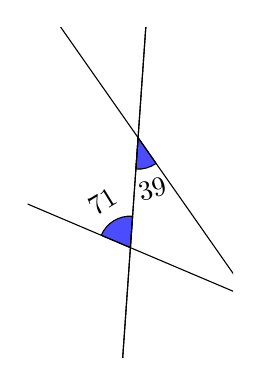
\begin{tikzpicture}[baseline,scale = 0.4]

    \tikzset{
      point/.style={
        thick,
        draw,
        cross out,
        inner sep=0pt,
        minimum width=5pt,
        minimum height=5pt,
      },
    }
    \clip (-3.3661492709735095,-4.989038226169209) rectangle (3.1568798497411326,5.487820251299121);
    	\draw  [color={black},preaction={fill,color = {blue},opacity = 0.7}] (0.7130893838392963,1.1759760562306565) -- (0.1395129474882508,1.9951281005196482) -- (0.06975647374412534,0.9975640502598244) arc (-93.77:-54.769999999999996:1) ;
	\draw[color={black}] (-28.539308870064048,42.95273031496924)--(29.391911201391594,-39.78162615821893);
	\draw[color={black}] (-3.348310739718021,-47.88307441247155)--(3.6970931084386485,52.87089466377067);
	\draw  [color={black},preaction={fill,color = {blue},opacity = 0.7}] (-1.0251395640686283,-1.1056149469004621) -- (-0.10463471061618831,-1.496346075389736) -- (-0.034878236872062915,-0.498782025129912) arc (85.69:156.69:1) ;
	\draw[color={black}] (-46.12987738323821,18.040210349073945)--(46.841112815458274,-21.42363362834269);
	\draw[color={black}] (-3.5924583978224613,-51.37454858838095)--(3.45294545033421,49.379420487861296);
	\draw [color={black}] (0.59,0.36) node[anchor = center,scale=1, rotate = 15.49952] {\ang{39}};
	\draw [color={black}] (-0.99,-0.05) node[anchor = center,scale=1, rotate = -328.49966] {\ang{71}};

\end{tikzpicture}\\ \end{minipage}
\end{enumerate}
\end{multicols}

\end{exercice}

\newpage

\section{Nommer les angles particuliers}

\begin{exercice}[1]
\begin{multicols}{3}
\begin{enumerate}
	\item \begin{minipage}[t]{\linewidth} Quel est l'angle alterne-interne à l'angle $\widehat{xDA}$ ?\\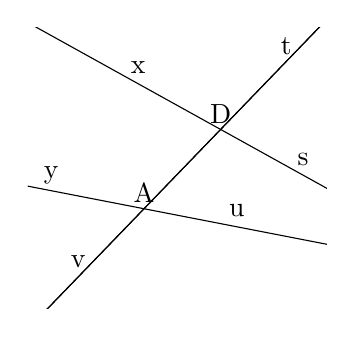
\begin{tikzpicture}[baseline,scale = 0.4]

    \tikzset{
      point/.style={
        thick,
        draw,
        cross out,
        inner sep=0pt,
        minimum width=5pt,
        minimum height=5pt,
      },
    }
    \clip (-4.736869106031488,-4.250328516779962) rectangle (4.7631758623361815,4.6700065683925605);
    	\draw[color={black}] (-42.34166861605179,25.679160612994153)--(45.99492180502718,-23.286611031885883);
	\draw[color={black}] (-33.343601782031854,-34.52831041625525)--(36.816893634326846,38.12500941794851);
	\draw[color={black}] (-50.123346728071695,8.461440068319265)--(49.02099880014237,-10.810268464711761);
	\draw[color={black}] (-35.77490607863836,-37.04599971744053)--(34.38558933772037,35.60732011676323);
	\draw [color={black}] (4.01,0.48) node[anchor = center,scale=1, rotate = 0] {s};
	\draw [color={black}] (-1.23,3.39) node[anchor = center,scale=1, rotate = 0] {x};
	\draw [color={black}] (3.47,4.1) node[anchor = center,scale=1, rotate = 0] {t};
	\draw [color={black}] (1.9,-1.15) node[anchor = center,scale=1, rotate = 0] {u};
	\draw [color={black}] (-3.99,-0.01) node[anchor = center,scale=1, rotate = 0] {y};
	\draw [color={black}] (-3.13,-2.74) node[anchor = center,scale=1, rotate = 0] {v};
	\draw [color={black}] (1.39,1.94) node[anchor = center,scale=1, rotate = 0] {D};
	\draw [color={black}] (-1.04,-0.58) node[anchor = center,scale=1, rotate = 0] {A};

\end{tikzpicture}\\ \end{minipage}
	\item \begin{minipage}[t]{\linewidth} Quel est l'angle alterne-interne à l'angle $\widehat{ADv}$ ?\\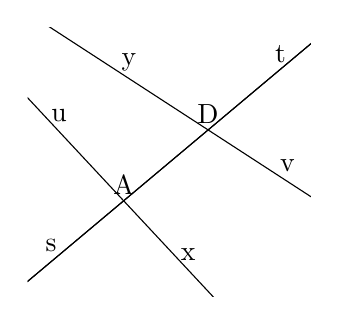
\begin{tikzpicture}[baseline,scale = 0.4]

    \tikzset{
      point/.style={
        thick,
        draw,
        cross out,
        inner sep=0pt,
        minimum width=5pt,
        minimum height=5pt,
      },
    }
    \clip (-4.197199994035402,-4.011010571846983) rectangle (4.798100590074228,4.532404376690253);
    	\draw[color={black}] (-40.40143951103323,28.51752697012443)--(44.30428785145457,-26.491015566393298);
	\draw[color={black}] (-36.770133269710925,-30.853805264953884)--(40.60035548530582,34.06774331338658);
	\draw[color={black}] (-35.24898466780339,35.603503666428715)--(33.632849698508956,-38.26322019710751);
	\draw[color={black}] (-39.45128882062737,-33.103561898856775)--(37.91919993438942,31.817986679483695);
	\draw [color={black}] (4.05,0.15) node[anchor = center,scale=1, rotate = 0] {v};
	\draw [color={black}] (-0.98,3.42) node[anchor = center,scale=1, rotate = 0] {y};
	\draw [color={black}] (3.83,3.71) node[anchor = center,scale=1, rotate = 0] {t};
	\draw [color={black}] (0.9,-2.66) node[anchor = center,scale=1, rotate = 0] {x};
	\draw [color={black}] (-3.2,1.73) node[anchor = center,scale=1, rotate = 0] {u};
	\draw [color={black}] (-3.45,-2.39) node[anchor = center,scale=1, rotate = 0] {s};
	\draw [color={black}] (1.53,1.79) node[anchor = center,scale=1, rotate = 0] {D};
	\draw [color={black}] (-1.15,-0.46) node[anchor = center,scale=1, rotate = 0] {A};

\end{tikzpicture}\\ \end{minipage}
	\item \begin{minipage}[t]{\linewidth} Quel est l'angle alterne-interne à l'angle $\widehat{BEy}$ ?\\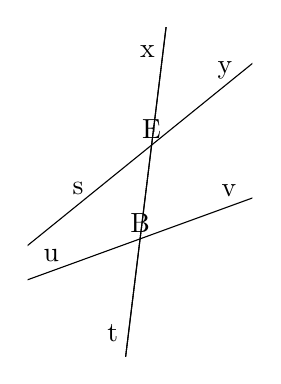
\begin{tikzpicture}[baseline,scale = 0.4]

    \tikzset{
      point/.style={
        thick,
        draw,
        cross out,
        inner sep=0pt,
        minimum width=5pt,
        minimum height=5pt,
      },
    }
    \clip (-3.751881877465446,-5.216457682385949) rectangle (3.3862738472500045,5.216457682385949);
    	\draw[color={black}] (-38.67449405774082,-29.977200325029884)--(39.81724804941324,33.584159171003684);
	\draw[color={black}] (-5.910663155149652,-48.13848835460412)--(6.3981405287702415,52.108672961169404);
	\draw[color={black}] (-47.16743505440314,-18.58982639374542)--(47.74151964497361,15.954208082147119);
	\draw[color={black}] (-6.276271185365095,-51.11612680952808)--(6.032532498554802,49.13103450624544);
	\draw [color={black}] (2.51,3.88) node[anchor = center,scale=1, rotate = 0] {y};
	\draw [color={black}] (-2.15,0.1) node[anchor = center,scale=1, rotate = 0] {s};
	\draw [color={black}] (0.05,4.47) node[anchor = center,scale=1, rotate = 0] {x};
	\draw [color={black}] (2.64,0.04) node[anchor = center,scale=1, rotate = 0] {v};
	\draw [color={black}] (-3,-2.01) node[anchor = center,scale=1, rotate = 0] {u};
	\draw [color={black}] (-1.05,-4.47) node[anchor = center,scale=1, rotate = 0] {t};
	\draw [color={black}] (0.18,1.99) node[anchor = center,scale=1, rotate = 0] {E};
	\draw [color={black}] (-0.18,-0.99) node[anchor = center,scale=1, rotate = 0] {B};

\end{tikzpicture}\\ \end{minipage}
	\item \begin{minipage}[t]{\linewidth} Quel est l'angle correspondant à l'angle $\widehat{uAt}$ ?\\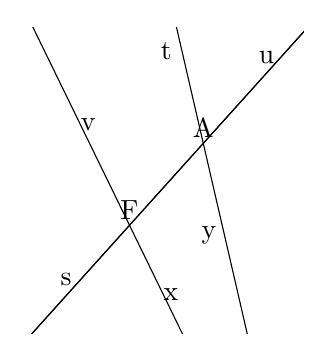
\begin{tikzpicture}[baseline,scale = 0.4]

    \tikzset{
      point/.style={
        thick,
        draw,
        cross out,
        inner sep=0pt,
        minimum width=5pt,
        minimum height=5pt,
      },
    }
    \clip (-4.571716929578387,-4.932671789852289) rectangle (4.199546898181071,4.787827432571796);
    	\draw[color={black}] (-10.243856807654957,49.83322047747786)--(12.476199681075396,-48.57815606583091);
	\draw[color={black}] (-32.45283440840463,-36.04252403565362)--(35.129356833840056,39.015103337563204);
	\draw[color={black}] (-23.256818552171588,43.45341266400355)--(21.01866727352523,-47.32478601221229);
	\draw[color={black}] (-34.79479153066063,-38.643530924824496)--(32.78739971158406,36.414096448392314);
	\draw [color={black}] (1.18,-1.81) node[anchor = center,scale=1, rotate = 0] {y};
	\draw [color={black}] (-0.17,4.04) node[anchor = center,scale=1, rotate = 0] {t};
	\draw [color={black}] (3.01,3.84) node[anchor = center,scale=1, rotate = 0] {u};
	\draw [color={black}] (-0.02,-3.68) node[anchor = center,scale=1, rotate = 0] {x};
	\draw [color={black}] (-2.65,1.71) node[anchor = center,scale=1, rotate = 0] {v};
	\draw [color={black}] (-3.35,-3.22) node[anchor = center,scale=1, rotate = 0] {s};
	\draw [color={black}] (1,1.61) node[anchor = center,scale=1, rotate = 0] {A};
	\draw [color={black}] (-1.34,-0.99) node[anchor = center,scale=1, rotate = 0] {F};

\end{tikzpicture}\\ \end{minipage}
	\item \begin{minipage}[t]{\linewidth} Quel est l'angle correspondant à l'angle $\widehat{yFu}$ ?\\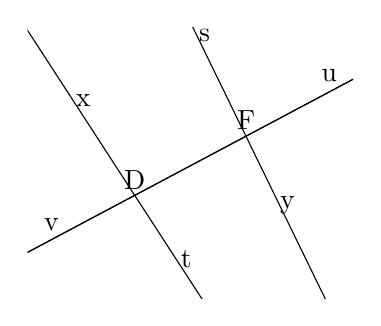
\begin{tikzpicture}[baseline,scale = 0.4]

    \tikzset{
      point/.style={
        thick,
        draw,
        cross out,
        inner sep=0pt,
        minimum width=5pt,
        minimum height=5pt,
      },
    }
    \clip (-5.164737964294635,-4.204954829408053) rectangle (5.164737964294635,4.385325264469283);
    	\draw[color={black}] (-20.152662153736017,45.878645440530136)--(24.122823671960802,-44.89955323568574);
	\draw[color={black}] (-42.381484457228495,-22.53463501372276)--(46.796222421523126,24.881992827652216);
	\draw[color={black}] (-28.997846936469212,40.99458527169941)--(26.010695600048535,-43.71114209078839);
	\draw[color={black}] (-45.9132748286642,-24.412521264866324)--(43.26443205008742,23.00410657650865);
	\draw [color={black}] (3.08,-1.26) node[anchor = center,scale=1, rotate = 0] {y};
	\draw [color={black}] (0.45,4.14) node[anchor = center,scale=1, rotate = 0] {s};
	\draw [color={black}] (4.41,2.85) node[anchor = center,scale=1, rotate = 0] {u};
	\draw [color={black}] (-0.13,-2.95) node[anchor = center,scale=1, rotate = 0] {t};
	\draw [color={black}] (-3.4,2.08) node[anchor = center,scale=1, rotate = 0] {x};
	\draw [color={black}] (-4.41,-1.85) node[anchor = center,scale=1, rotate = 0] {v};
	\draw [color={black}] (1.77,1.44) node[anchor = center,scale=1, rotate = 0] {F};
	\draw [color={black}] (-1.77,-0.44) node[anchor = center,scale=1, rotate = 0] {D};

\end{tikzpicture}\\ \end{minipage}
	\item \begin{minipage}[t]{\linewidth} Quel est l'angle alterne-interne à l'angle $\widehat{FCu}$ ?\\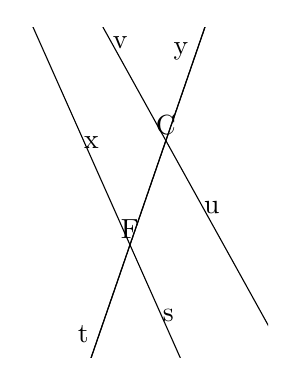
\begin{tikzpicture}[baseline,scale = 0.4]

    \tikzset{
      point/.style={
        thick,
        draw,
        cross out,
        inner sep=0pt,
        minimum width=5pt,
        minimum height=5pt,
      },
    }
    \clip (-3.7367342083748936,-5.004833590196926) rectangle (3.8946672956702804,5.4775928779965835);
    	\draw[color={black}] (-23.589344703402542,45.622022508168406)--(25.376426941477508,-42.71456791291054);
	\draw[color={black}] (-15.627271413943522,-45.38489162876719)--(17.255112186229304,50.11248450676377);
	\draw[color={black}] (-20.825184385475744,44.25899501873106)--(20.255216565180074,-48.009096203171616);
	\draw[color={black}] (-16.766759954543573,-48.694206643364815)--(16.11562364562926,46.80316949216618);
	\draw [color={black}] (2.11,-0.23) node[anchor = center,scale=1, rotate = 0] {u};
	\draw [color={black}] (-0.8,5.01) node[anchor = center,scale=1, rotate = 0] {v};
	\draw [color={black}] (1.13,4.73) node[anchor = center,scale=1, rotate = 0] {y};
	\draw [color={black}] (0.73,-3.66) node[anchor = center,scale=1, rotate = 0] {s};
	\draw [color={black}] (-1.71,1.82) node[anchor = center,scale=1, rotate = 0] {x};
	\draw [color={black}] (-1.97,-4.25) node[anchor = center,scale=1, rotate = 0] {t};
	\draw [color={black}] (0.65,2.39) node[anchor = center,scale=1, rotate = 0] {C};
	\draw [color={black}] (-0.49,-0.92) node[anchor = center,scale=1, rotate = 0] {F};

\end{tikzpicture}\\ \end{minipage}
	\item \begin{minipage}[t]{\linewidth} Quel est l'angle correspondant à l'angle $\widehat{uDx}$ ?\\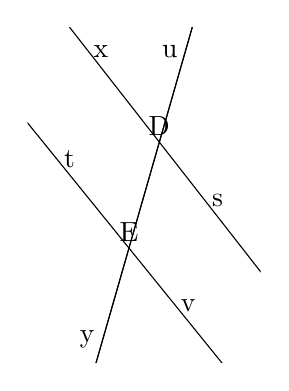
\begin{tikzpicture}[baseline,scale = 0.4]

    \tikzset{
      point/.style={
        thick,
        draw,
        cross out,
        inner sep=0pt,
        minimum width=5pt,
        minimum height=5pt,
      },
    }
    \clip (-3.6293280315809087,-5.075677631722435) rectangle (3.770040923495027,5.5563084796915945);
    	\draw[color={black}] (-30.231799054648906,41.323061072212724)--(31.95000995324256,-38.26602504206617);
	\draw[color={black}] (-13.230593079215955,-46.14056140503931)--(14.608779858300952,50.9468698847309);
	\draw[color={black}] (-31.879475586217374,37.41540552894106)--(31.681883909816214,-41.07633657821299);
	\draw[color={black}] (-14.195323824575457,-49.50497734082342)--(13.64404911294146,47.582453948946785);
	\draw [color={black}] (2.4,0.06) node[anchor = center,scale=1, rotate = 0] {s};
	\draw [color={black}] (-1.3,4.79) node[anchor = center,scale=1, rotate = 0] {x};
	\draw [color={black}] (0.88,4.81) node[anchor = center,scale=1, rotate = 0] {u};
	\draw [color={black}] (1.47,-3.27) node[anchor = center,scale=1, rotate = 0] {v};
	\draw [color={black}] (-2.3,1.39) node[anchor = center,scale=1, rotate = 0] {t};
	\draw [color={black}] (-1.74,-4.33) node[anchor = center,scale=1, rotate = 0] {y};
	\draw [color={black}] (0.55,2.42) node[anchor = center,scale=1, rotate = 0] {D};
	\draw [color={black}] (-0.41,-0.94) node[anchor = center,scale=1, rotate = 0] {E};

\end{tikzpicture}\\ \end{minipage}
	\item \begin{minipage}[t]{\linewidth} Quel est l'angle alterne-interne à l'angle $\widehat{ECv}$ ?\\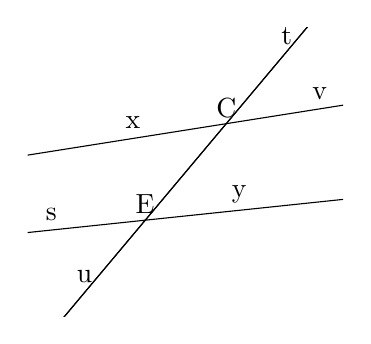
\begin{tikzpicture}[baseline,scale = 0.4]

    \tikzset{
      point/.style={
        thick,
        draw,
        cross out,
        inner sep=0pt,
        minimum width=5pt,
        minimum height=5pt,
      },
    }
    \clip (-5.019140905477899,-4.583099794098132) rectangle (4.998640241158492,4.58022221559489);
    	\draw[color={black}] (-48.098841810383796,-6.289634365773592)--(51.65768058972509,9.510246603289735);
	\draw[color={black}] (-30.853805264953884,-36.770133269710925)--(34.06774331338658,40.60035548530582);
	\draw[color={black}] (-51.011669987786746,-6.758512049620633)--(49.43504144440886,3.7988627404123747);
	\draw[color={black}] (-33.42495570370005,-39.83431104218686)--(31.49659287464043,37.536177712829925);
	\draw [color={black}] (4.25,2.5) node[anchor = center,scale=1, rotate = 0] {v};
	\draw [color={black}] (-1.68,1.56) node[anchor = center,scale=1, rotate = 0] {x};
	\draw [color={black}] (3.21,4.33) node[anchor = center,scale=1, rotate = 0] {t};
	\draw [color={black}] (1.7,-0.72) node[anchor = center,scale=1, rotate = 0] {y};
	\draw [color={black}] (-4.27,-1.35) node[anchor = center,scale=1, rotate = 0] {s};
	\draw [color={black}] (-3.21,-3.33) node[anchor = center,scale=1, rotate = 0] {u};
	\draw [color={black}] (1.29,2.03) node[anchor = center,scale=1, rotate = 0] {C};
	\draw [color={black}] (-1.29,-1.03) node[anchor = center,scale=1, rotate = 0] {E};

\end{tikzpicture}\\ \end{minipage}
	\item \begin{minipage}[t]{\linewidth} Quel est l'angle alterne-interne à l'angle $\widehat{DEu}$ ?\\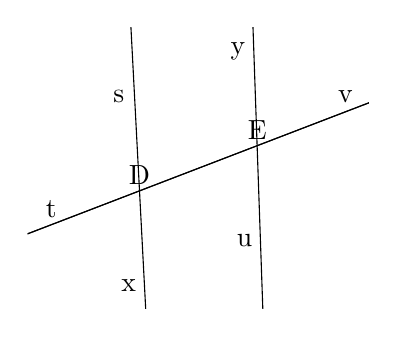
\begin{tikzpicture}[baseline,scale = 0.4]

    \tikzset{
      point/.style={
        thick,
        draw,
        cross out,
        inner sep=0pt,
        minimum width=5pt,
        minimum height=5pt,
      },
    }
    \clip (-5.417902132486009,-4.462624503354323) rectangle (5.417902132486009,4.464908380147888);
    	\draw[color={black}] (0.12218601786934635,50.68627725004538)--(3.647035184821962,-50.252196278883275);
	\draw[color={black}] (-44.81186047186567,-17.201661578174413)--(49.47976260435168,18.993501325900915);
	\draw[color={black}] (-4.483958665141602,49.21474083863809)--(0.8019729153957385,-51.646842171573866);
	\draw[color={black}] (-48.54618217785449,-18.635133376355615)--(45.74544089836289,17.560029527719713);
	\draw [color={black}] (1.47,-2.28) node[anchor = center,scale=1, rotate = 0] {u};
	\draw [color={black}] (1.26,3.71) node[anchor = center,scale=1, rotate = 0] {y};
	\draw [color={black}] (4.67,2.29) node[anchor = center,scale=1, rotate = 0] {v};
	\draw [color={black}] (-2.21,-3.71) node[anchor = center,scale=1, rotate = 0] {x};
	\draw [color={black}] (-2.52,2.28) node[anchor = center,scale=1, rotate = 0] {s};
	\draw [color={black}] (-4.67,-1.29) node[anchor = center,scale=1, rotate = 0] {t};
	\draw [color={black}] (1.87,1.22) node[anchor = center,scale=1, rotate = 0] {E};
	\draw [color={black}] (-1.87,-0.22) node[anchor = center,scale=1, rotate = 0] {D};

\end{tikzpicture}\\ \end{minipage}
\end{enumerate}
\end{multicols}

\end{exercice}


\end{document}
\textbf{Les angles marqués sont-ils alternes-internes, correspondants ou ni l'un, ni l'autre ?}
\begin{multicols}{3}
\begin{enumerate}
	\item \begin{minipage}[t]{\linewidth} 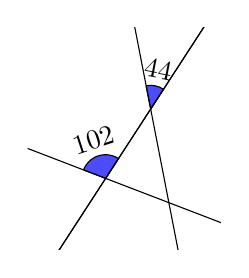
\begin{tikzpicture}[baseline,scale = 0.3]

    \tikzset{
      point/.style={
        thick,
        draw,
        cross out,
        inner sep=0pt,
        minimum width=5pt,
        minimum height=5pt,
      },
    }
    \clip (-4.390019349521659,-4.69335283972712) rectangle (3.78572476438357,4.702887402261128);
    	\draw  [color={black},preaction={fill,color = {blue},opacity = 0.7}] (0.626149557145996,2.2396330353657996) -- (0.8169585525225405,1.2580058519181354) -- (1.3615975875375679,2.0966764198635595) arc (56.72:100.72:1) ;
	\draw[color={black}] (-8.723491216304707,50.33936502430133)--(10.548217316726333,-48.804980503912724);
	\draw[color={black}] (-26.414993198228814,-40.67552254535305)--(28.59354933828892,44.030204817134745);
	\draw  [color={black},preaction={fill,color = {blue},opacity = 0.7}] (-2.0228584965272556,-1.3189731863455467) -- (-1.0892780700300544,-1.6773411358908479) -- (-0.5446390350150268,-0.8386705679454244) arc (56.72:158.72:1) ;
	\draw[color={black}] (-47.76829939489014,16.241056341374165)--(46.523323681327234,-19.954106562701163);
	\draw[color={black}] (-28.321229820781415,-43.610869533162045)--(26.687312715736333,41.094857829325775);
	\draw [color={black}] (1.14,2.93) node[anchor = center,scale=1, rotate = -10.995039999999989] {\ang{44}};
	\draw [color={black}] (-1.61,-0.06) node[anchor = center,scale=1, rotate = -341.99936] {\ang{102}};

\end{tikzpicture}\\ \end{minipage}
	\item \begin{minipage}[t]{\linewidth} 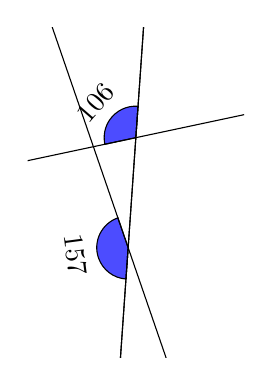
\begin{tikzpicture}[baseline,scale = 0.4]

    \tikzset{
      point/.style={
        thick,
        draw,
        cross out,
        inner sep=0pt,
        minimum width=5pt,
        minimum height=5pt,
      },
    }
    \clip (-3.329808091585229,-5.487820251299121) rectangle (3.539077512817605,4.989038226169209);
    	\draw  [color={black},preaction={fill,color = {blue},opacity = 0.7}] (-0.8735128901176171,1.2884343845719772) -- (0.1046347106161884,1.4963460753897364) -- (0.17439118436031364,2.4939101256495606) arc (85.69:191.69:1) ;
	\draw[color={black}] (-48.802745326074096,-8.899238465498234)--(49.99016234804028,12.099842307095466);
	\draw[color={black}] (-3.3831889765900853,-48.381856437601485)--(3.662214871566587,52.372112638640786);
	\draw  [color={black},preaction={fill,color = {blue},opacity = 0.7}] (-0.20926942123237727,-2.992692150779473) -- (-0.1395129474882513,-1.9951281005196484) -- (-0.4650811019454078,-1.0496095249203314) arc (109.17:266.17:1) ;
	\draw[color={black}] (-16.41792067034609,45.280800679446195)--(16.464462929826745,-50.21657545608481);
	\draw[color={black}] (-3.627336634694524,-51.87333061351086)--(3.4180672134621473,48.88063846273138);
	\draw [color={black}] (-1.18,2.61) node[anchor = center,scale=1, rotate = -311.0002] {\ang{106}};
	\draw [color={black}] (-1.82,-2.22) node[anchor = center,scale=1, rotate = -82.50011] {\ang{157}};

\end{tikzpicture}\\ \end{minipage}
	\item \begin{minipage}[t]{\linewidth} 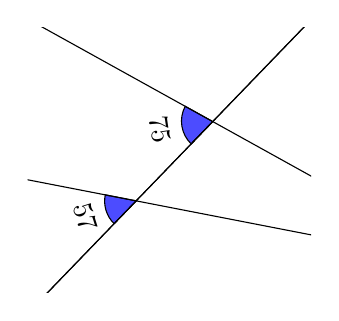
\begin{tikzpicture}[baseline,scale = 0.4]

    \tikzset{
      point/.style={
        thick,
        draw,
        cross out,
        inner sep=0pt,
        minimum width=5pt,
        minimum height=5pt,
      },
    }
    \clip (-4.486869106031488,-4.000328516779962) rectangle (4.5131758623361815,4.4200065683925605);
    	\draw  [color={black},preaction={fill,color = {blue},opacity = 0.7}] (0.6946583704589984,0.7193398003386509) -- (1.3893167409179954,1.4386796006773026) -- (0.5146970337785991,1.9234892209236392) arc (151.86:226.86:1) ;
	\draw[color={black}] (-42.34166861605179,25.679160612994153)--(45.99492180502718,-23.286611031885883);
	\draw[color={black}] (-33.343601782031854,-34.52831041625525)--(36.816893634326846,38.12500941794851);
	\draw  [color={black},preaction={fill,color = {blue},opacity = 0.7}] (-1.7366459261474938,-1.798349500846627) -- (-1.0419875556884963,-1.0790097005079757) -- (-2.0236147391361605,-0.8882007051314311) arc (168.54:225.54:1) ;
	\draw[color={black}] (-50.123346728071695,8.461440068319265)--(49.02099880014237,-10.810268464711761);
	\draw[color={black}] (-35.77490607863836,-37.04599971744053)--(34.38558933772037,35.60732011676323);
	\draw [color={black}] (-0.29,1.19) node[anchor = center,scale=1, rotate = -81.50019] {\ang{75}};
	\draw [color={black}] (-2.66,-1.59) node[anchor = center,scale=1, rotate = -72.49962] {\ang{57}};

\end{tikzpicture}\\ \end{minipage}
	\item \begin{minipage}[t]{\linewidth} 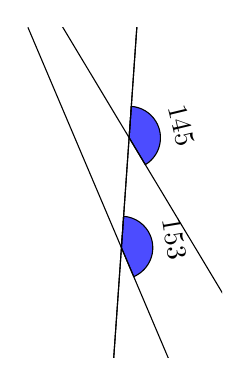
\begin{tikzpicture}[baseline,scale = 0.4]

    \tikzset{
      point/.style={
        thick,
        draw,
        cross out,
        inner sep=0pt,
        minimum width=5pt,
        minimum height=5pt,
      },
    }
    \clip (-3.081320233229482,-4.989038226169209) rectangle (3.0925418121643005,5.487820251299121);
    	\draw  [color={black},preaction={fill,color = {blue},opacity = 0.7}] (0.20926942123237668,2.992692150779472) -- (0.1395129474882511,1.9951281005196482) -- (0.6545510223983052,1.1379607998175363) arc (-58.68:86.32:1) ;
	\draw[color={black}] (-25.612390798014463,44.85349313562526)--(26.406454767901018,-41.72040423528807);
	\draw[color={black}] (-3.348310739718021,-47.88307441247155)--(3.6970931084386485,52.87089466377067);
	\draw  [color={black},preaction={fill,color = {blue},opacity = 0.7}] (-0.034878236872062596,-0.4987820251299113) -- (-0.10463471061618815,-1.496346075389736) -- (0.2860964178730856,-2.4168509288421767) arc (-66.73:86.27:1) ;
	\draw[color={black}] (-19.641191135079886,44.52889659723229)--(19.822652842336783,-48.44209360146421);
	\draw[color={black}] (-3.5924583978224613,-51.37454858838095)--(3.45294545033421,49.379420487861296);
	\draw [color={black}] (1.79,2.39) node[anchor = center,scale=1, rotate = -76.50006] {\ang{145}};
	\draw [color={black}] (1.57,-1.22) node[anchor = center,scale=1, rotate = -80.50002] {\ang{153}};

\end{tikzpicture}\\ \end{minipage}
	\item \begin{minipage}[t]{\linewidth} 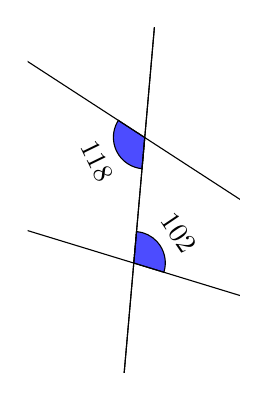
\begin{tikzpicture}[baseline,scale = 0.4]

    \tikzset{
      point/.style={
        thick,
        draw,
        cross out,
        inner sep=0pt,
        minimum width=5pt,
        minimum height=5pt,
      },
    }
    \clip (-3.543225753384422,-5.480973490458728) rectangle (3.1946027823937895,5.480973490458728);
    	\draw  [color={black},preaction={fill,color = {blue},opacity = 0.7}] (0.08715574274765758,0.9961946980917454) -- (0.17431148549531622,1.9923893961834909) -- (-0.6643590824501077,2.537028431198518) arc (147.48:265.48:1) ;
	\draw[color={black}] (-41.75921691177589,29.22434114693484)--(42.94651045071194,-25.784201389582886);
	\draw[color={black}] (-4.183475651887591,-47.8173455084038)--(4.619254365625881,52.79831899886253);
	\draw  [color={black},preaction={fill,color = {blue},opacity = 0.7}] (-0.08715574274765814,-0.9961946980917457) -- (-0.17431148549531658,-1.992389396183491) -- (0.7819932704677189,-2.284761100906228) arc (-17.25:84.75:1) ;
	\draw[color={black}] (-47.98954928364709,12.626195839953347)--(48.597231068619486,-16.903346337043065);
	\draw[color={black}] (-4.532098622878223,-51.80212430077077)--(4.270631394635249,48.81354020649553);
	\draw [color={black}] (-1.35,1.25) node[anchor = center,scale=1, rotate = -64.00014] {\ang{118}};
	\draw [color={black}] (1.24,-1.04) node[anchor = center,scale=1, rotate = -55.999719999999996] {\ang{102}};

\end{tikzpicture}\\ \end{minipage}
	\item \begin{minipage}[t]{\linewidth} 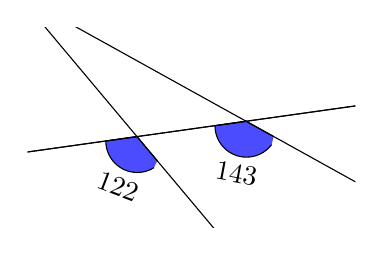
\begin{tikzpicture}[baseline,scale = 0.4]

    \tikzset{
      point/.style={
        thick,
        draw,
        cross out,
        inner sep=0pt,
        minimum width=5pt,
        minimum height=5pt,
      },
    }
    \clip (-4.956206309337067,-3.0958463764853414) rectangle (5.451340343707852,3.249879544778853);
    	\draw  [color={black},preaction={fill,color = {blue},opacity = 0.7}] (2.8551558446225362,-0.20646341832620585) -- (1.9805361374831405,0.27834620192013104) -- (0.9902680687415701,0.13917310096006552) arc (-180:-37:1) ;
	\draw[color={black}] (-41.75044921948663,24.518827214236982)--(46.58614120159231,-24.446944430643057);
	\draw[color={black}] (-47.53286729959539,-6.680308846083142)--(52.48420764330324,7.37617435088347);
	\draw  [color={black},preaction={fill,color = {blue},opacity = 0.7}] (-0.842614493425816,-0.9748040945590766) -- (-1.4854021031123552,-0.20875965144009823) -- (-2.475670171853926,-0.34793275240016364) arc (-180:-58:1) ;
	\draw[color={black}] (-33.62478258743933,38.09346250450881)--(31.296765990901154,-39.27702625050798);
	\draw[color={black}] (-50.99880554019087,-7.16741469944337)--(49.01826940270773,6.889068497523239);
	\draw [color={black}] (1.67,-1.39) node[anchor = center,scale=1, rotate = -10.49892] {\ang{143}};
	\draw [color={black}] (-2.09,-1.8) node[anchor = center,scale=1, rotate = -20.99966] {\ang{122}};

\end{tikzpicture}\\ \end{minipage}
	\item \begin{minipage}[t]{\linewidth} 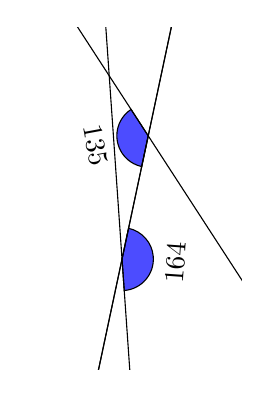
\begin{tikzpicture}[baseline,scale = 0.4]

    \tikzset{
      point/.style={
        thick,
        draw,
        cross out,
        inner sep=0pt,
        minimum width=5pt,
        minimum height=5pt,
      },
    }
    \clip (-3.4116822670772207,-5.448987352247084) rectangle (3.387356724494242,5.390738003669028);
    	\draw  [color={black},preaction={fill,color = {blue},opacity = 0.7}] (0.20791169081775973,0.9781476007338062) -- (0.4158233816355189,1.9562952014676114) -- (-0.12881565337950807,2.794965769413035) arc (123.28:258.28:1) ;
	\draw[color={black}] (-26.816128369115834,43.8898235987388)--(28.1924141674019,-40.815903763749);
	\draw[color={black}] (-9.979761159252451,-46.95108483522266)--(11.01931961334125,51.84182283889169);
	\draw  [color={black},preaction={fill,color = {blue},opacity = 0.7}] (-0.20791169081775984,-0.9781476007338058) -- (-0.4158233816355195,-1.9562952014676112) -- (-0.3460669078913941,-2.9538592517274354) arc (-85.69:78.31:1) ;
	\draw[color={black}] (-3.903647068841793,47.9219073115236)--(3.1417567793148793,-52.832061764718645);
	\draw[color={black}] (-10.811407922523491,-50.86367523815789)--(10.187672850070213,47.92923243595647);
	\draw [color={black}] (-1.26,1.65) node[anchor = center,scale=1, rotate = -79.4997] {\ang{135}};
	\draw [color={black}] (1.28,-2.07) node[anchor = center,scale=1, rotate = 85.99994] {\ang{164}};

\end{tikzpicture}\\ \end{minipage}
	\item \begin{minipage}[t]{\linewidth} 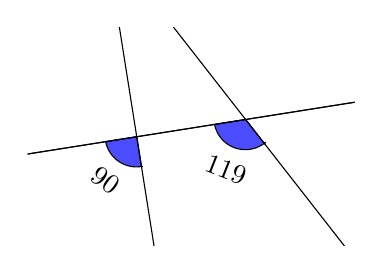
\begin{tikzpicture}[baseline,scale = 0.4]

    \tikzset{
      point/.style={
        thick,
        draw,
        cross out,
        inner sep=0pt,
        minimum width=5pt,
        minimum height=5pt,
      },
    }
    \clip (-4.94459753267812,-3.6977167193457596) rectangle (5.438441702975689,3.228413324225068);
    	\draw  [color={black},preaction={fill,color = {blue},opacity = 0.7}] (2.5910381565159337,-0.4751418235262608) -- (1.9753766811902758,0.3128689300804615) -- (0.9876883405951378,0.15643446504023095) arc (-168.54:-49.53999999999999:1) ;
	\draw[color={black}] (-28.807697085092634,39.71340661041656)--(33.374111922798846,-39.87567950386236);
	\draw[color={black}] (-47.40904034856661,-7.508854321931083)--(52.3474820515423,8.291026647132238);
	\draw  [color={black},preaction={fill,color = {blue},opacity = 0.7}] (-1.3250980458524761,-1.2223400381554839) -- (-1.4815325108927069,-0.234651697560346) -- (-2.4692208514878446,-0.3910861626005768) arc (-168.54:-78.53999999999999:1) ;
	\draw[color={black}] (-9.303255762904255,49.149765332196544)--(6.496625206159072,-50.606757067912376);
	\draw[color={black}] (-50.865949540649595,-8.05637494957189)--(48.89057285945932,7.743506019491428);
	\draw [color={black}] (1.35,-1.27) node[anchor = center,scale=1, rotate = -21.49967] {\ang{119}};
	\draw [color={black}] (-2.48,-1.61) node[anchor = center,scale=1, rotate = -36.00042] {\ang{90}};

\end{tikzpicture}\\ \end{minipage}
	\item \begin{minipage}[t]{\linewidth} 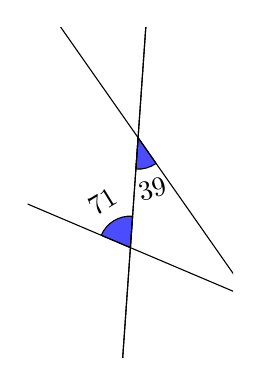
\begin{tikzpicture}[baseline,scale = 0.4]

    \tikzset{
      point/.style={
        thick,
        draw,
        cross out,
        inner sep=0pt,
        minimum width=5pt,
        minimum height=5pt,
      },
    }
    \clip (-3.3661492709735095,-4.989038226169209) rectangle (3.1568798497411326,5.487820251299121);
    	\draw  [color={black},preaction={fill,color = {blue},opacity = 0.7}] (0.7130893838392963,1.1759760562306565) -- (0.1395129474882508,1.9951281005196482) -- (0.06975647374412534,0.9975640502598244) arc (-93.77:-54.769999999999996:1) ;
	\draw[color={black}] (-28.539308870064048,42.95273031496924)--(29.391911201391594,-39.78162615821893);
	\draw[color={black}] (-3.348310739718021,-47.88307441247155)--(3.6970931084386485,52.87089466377067);
	\draw  [color={black},preaction={fill,color = {blue},opacity = 0.7}] (-1.0251395640686283,-1.1056149469004621) -- (-0.10463471061618831,-1.496346075389736) -- (-0.034878236872062915,-0.498782025129912) arc (85.69:156.69:1) ;
	\draw[color={black}] (-46.12987738323821,18.040210349073945)--(46.841112815458274,-21.42363362834269);
	\draw[color={black}] (-3.5924583978224613,-51.37454858838095)--(3.45294545033421,49.379420487861296);
	\draw [color={black}] (0.59,0.36) node[anchor = center,scale=1, rotate = 15.49952] {\ang{39}};
	\draw [color={black}] (-0.99,-0.05) node[anchor = center,scale=1, rotate = -328.49966] {\ang{71}};

\end{tikzpicture}\\ \end{minipage}
\end{enumerate}
\end{multicols}
\message{ !name(FA-02-ex01.tex)}
\message{ !name(FA-02-ex01.tex) !offset(-2) }
lticols}{3}
\begin{enumerate}
	\item \begin{minipage}[t]{\linewidth} 
\message{ !name(FA-02-ex01.tex) !offset(-6) }
\begin{multicols}{3}
\begin{enumerate}
	\item \begin{minipage}[t]{\linewidth} Marquer en rouge l'angle alterne-interne à l'angle marqué en bleu.\\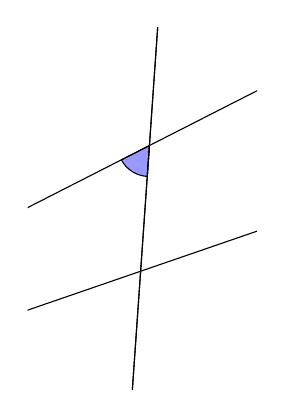
\begin{tikzpicture}[baseline,scale = 0.4]

    \tikzset{
      point/.style={
        thick,
        draw,
        cross out,
        inner sep=0pt,
        minimum width=5pt,
        minimum height=5pt,
      },
    }
    \clip (-3.7260686742862017,-5.737820251299121) rectangle (3.5625325200533546,5.737820251299121);
    	\draw  [color={black},preaction={fill,color = {blue},opacity = 0.4}] (0.06975647374412497,0.9975640502598244) -- (0.13951294748825063,1.995128100519648) -- (-0.7514935767001168,1.5411376007801016) arc (-151.86:-92.86000000000001:1) ;
	\draw[color={black}] (-44.41081326193014,-20.70439688645769)--(45.580845681095006,25.14864358723653);
	\draw[color={black}] (-3.348310739718021,-47.88307441247155)--(3.6970931084386485,52.87089466377067);
	\draw[color={black}] (-47.415441727454095,-18.273535823377483)--(48.08193440807691,14.608847776795344);
	\draw[color={black}] (-3.627336634694524,-51.87333061351086)--(3.4180672134621473,48.88063846273138);

\end{tikzpicture}\\ \end{minipage}
	\item \begin{minipage}[t]{\linewidth} Marquer en rouge l'angle alterne-interne à l'angle marqué en bleu.\\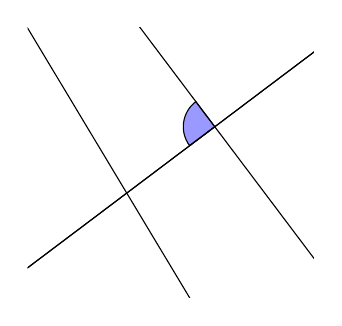
\begin{tikzpicture}[baseline,scale = 0.4]

    \tikzset{
      point/.style={
        thick,
        draw,
        cross out,
        inner sep=0pt,
        minimum width=5pt,
        minimum height=5pt,
      },
    }
    \clip (-4.343859795212818,-4.224224436834409) rectangle (4.743177550236464,4.349536576445975);
    	\draw  [color={black},preaction={fill,color = {blue},opacity = 0.4}] (0.798635510047293,0.6018150231520484) -- (1.5972710200945857,1.2036300463040968) -- (0.9954559969425373,2.0022655563513894) arc (127.02:217.01999999999998:1) ;
	\draw[color={black}] (-28.49348013750784,41.13540554866874)--(32.289837200849064,-39.52678096610784);
	\draw[color={black}] (-38.334504482270056,-28.887121111298317)--(42.32768203250652,31.896196227058557);
	\draw[color={black}] (-26.94985701057366,41.95564250037754)--(25.068988555341836,-44.6182548705358);
	\draw[color={black}] (-41.12972876743558,-30.993473692330483)--(39.532457747341,29.789843646026387);

\end{tikzpicture}\\ \end{minipage}
	\item \begin{minipage}[t]{\linewidth} Marquer en rouge l'angle correspondant à l'angle marqué en bleu.\\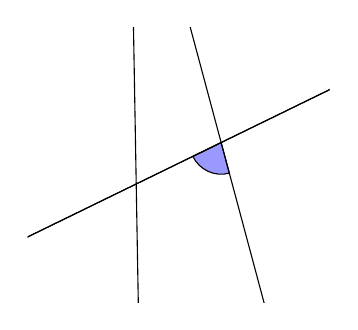
\begin{tikzpicture}[baseline,scale = 0.4]

    \tikzset{
      point/.style={
        thick,
        draw,
        cross out,
        inner sep=0pt,
        minimum width=5pt,
        minimum height=5pt,
      },
    }
    \clip (-4.794573208346252,-4.4070998056527895) rectangle (4.794573208346252,4.305334199050821);
    	\draw  [color={black},preaction={fill,color = {blue},opacity = 0.4}] (1.6070101145512712,-0.30836910610545204) -- (1.3481910694487507,0.6575567201836161) -- (0.4493970231495838,0.2191855733945388) arc (-154.32:-75.32:1) ;
	\draw[color={black}] (-11.592761185677286,48.953848034637026)--(14.547962369677307,-48.604660420558865);
	\draw[color={black}] (-43.59151124550959,-21.261000619270252)--(47.18668743070626,23.014485206426563);
	\draw[color={black}] (-2.220811391312921,49.33482803763595)--(-0.4581183411472969,-51.64978917315957);
	\draw[color={black}] (-46.287893384407106,-22.576114059637487)--(44.49030529180877,21.699371766059333);

\end{tikzpicture}\\ \end{minipage}
	\item \begin{minipage}[t]{\linewidth} Marquer en rouge l'angle correspondant à l'angle marqué en bleu.\\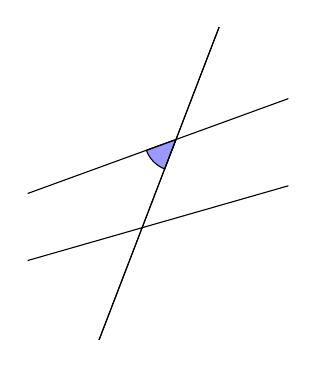
\begin{tikzpicture}[baseline,scale = 0.4]

    \tikzset{
      point/.style={
        thick,
        draw,
        cross out,
        inner sep=0pt,
        minimum width=5pt,
        minimum height=5pt,
      },
    }
    \clip (-4.171337012132907,-4.951111919237407) rectangle (4.106629786675676,4.951111919237408);
    	\draw  [color={black},preaction={fill,color = {blue},opacity = 0.4}] (0.1791839747726499,0.46679021324860104) -- (0.5375519243179505,1.4003706397458024) -- (-0.40214069646795797,1.0583504964201342) arc (-160.13:-111.13:1) ;
	\draw[color={black}] (-46.44707911497747,-15.700636526537632)--(48.46187558439928,18.843397949354905);
	\draw[color={black}] (-17.38084555294707,-45.27865068511428)--(18.814317351128267,49.012972391103084);
	\draw[color={black}] (-48.6006367212339,-15.182238430595756)--(48.48679456853631,12.657134506921151);
	\draw[color={black}] (-18.45594940158297,-48.07939196460589)--(17.739213502492365,46.21223111161149);

\end{tikzpicture}\\ \end{minipage}
	\item \begin{minipage}[t]{\linewidth} Marquer en rouge l'angle alterne-interne à l'angle marqué en bleu.\\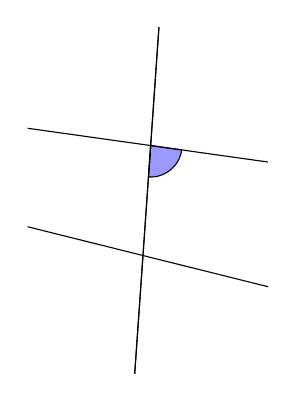
\begin{tikzpicture}[baseline,scale = 0.4]

    \tikzset{
      point/.style={
        thick,
        draw,
        cross out,
        inner sep=0pt,
        minimum width=5pt,
        minimum height=5pt,
      },
    }
    \clip (-3.800400126316241,-5.737820251299121) rectangle (3.8254389168408993,5.239038226169209);
    	\draw  [color={black},preaction={fill,color = {blue},opacity = 0.4}] (1.0949027793577586,1.357172974429671) -- (0.10463471061618787,1.4963460753897364) -- (0.03487823687206258,0.49878202512991177) arc (-93.77:-7.769999999999996:1) ;
	\draw[color={black}] (-49.40876872646233,8.455001123393007)--(50.608306216436276,-5.6014820735736);
	\draw[color={black}] (-3.3831889765900853,-48.381856437601485)--(3.662214871566587,52.372112638640786);
	\draw[color={black}] (-48.654299261288074,10.100966679463742)--(49.34556909258757,-14.333144776102706);
	\draw[color={black}] (-3.627336634694524,-51.87333061351086)--(3.4180672134621473,48.88063846273138);

\end{tikzpicture}\\ \end{minipage}
	\item \begin{minipage}[t]{\linewidth} Marquer en rouge l'angle alterne-interne à l'angle marqué en bleu.\\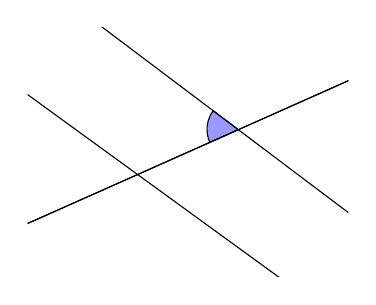
\begin{tikzpicture}[baseline,scale = 0.4]

    \tikzset{
      point/.style={
        thick,
        draw,
        cross out,
        inner sep=0pt,
        minimum width=5pt,
        minimum height=5pt,
      },
    }
    \clip (-4.860954559391704,-3.8507921867397643) rectangle (5.317727288213004,4.0525454408018);
    	\draw  [color={black},preaction={fill,color = {blue},opacity = 0.4}] (0.9135454576426014,0.4067366430758005) -- (1.827090915285202,0.8134732861516007) -- (1.0284554052379091,1.4152883093036486) arc (143.61:204.61:1) ;
	\draw[color={black}] (-38.104684587079426,30.90422444375401)--(42.557501927697125,-29.879092894602856);
	\draw[color={black}] (-43.85018196684482,-19.523358867638407)--(48.41790925505783,21.557042083017407);
	\draw[color={black}] (-41.821167905211276,28.779157650009957)--(39.889548526658416,-30.58715283152983);
	\draw[color={black}] (-47.047591068593945,-20.946937118403707)--(45.22050015330874,20.133463832252104);

\end{tikzpicture}\\ \end{minipage}
	\item \begin{minipage}[t]{\linewidth} Marquer en rouge l'angle alterne-interne à l'angle marqué en bleu.\\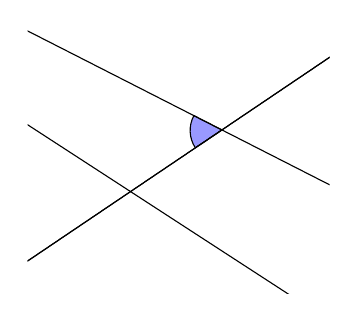
\begin{tikzpicture}[baseline,scale = 0.4]

    \tikzset{
      point/.style={
        thick,
        draw,
        cross out,
        inner sep=0pt,
        minimum width=5pt,
        minimum height=5pt,
      },
    }
    \clip (-4.509568062668835,-4.088724624415212) rectangle (5.081094717675187,4.3652149642586675);
    	\draw  [color={black},preaction={fill,color = {blue},opacity = 0.4}] (0.8290375725550416,0.5591929034707473) -- (1.658075145110083,1.1183858069414938) -- (0.7670686209217156,1.5723763066810406) arc (151.86:212.86:1) ;
	\draw[color={black}] (-42.892251064308304,23.81791079391883)--(47.09940787871684,-22.03512967977539);
	\draw[color={black}] (-39.793803482642,-26.841259366595846)--(43.93899134541721,29.63722388394958);
	\draw[color={black}] (-43.17708475610377,26.39316239554524)--(41.52864260638407,-28.61538014097251);
	\draw[color={black}] (-42.695434986584644,-28.798434528743467)--(41.03735984147456,27.680048721801974);

\end{tikzpicture}\\ \end{minipage}
	\item \begin{minipage}[t]{\linewidth} Marquer en rouge l'angle correspondant à l'angle marqué en bleu.\\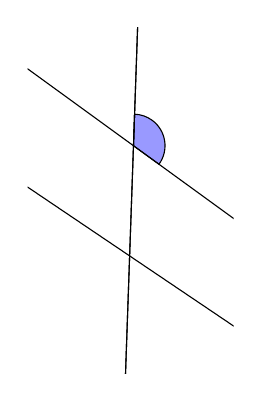
\begin{tikzpicture}[baseline,scale = 0.4]

    \tikzset{
      point/.style={
        thick,
        draw,
        cross out,
        inner sep=0pt,
        minimum width=5pt,
        minimum height=5pt,
      },
    }
    \clip (-3.2894619627188773,-5.247258721585931) rectangle (3.2468499765298446,5.7469541350954785);
    	\draw  [color={black},preaction={fill,color = {blue},opacity = 0.4}] (0.10469849010750315,2.9981724810572867) -- (0.06979899340500217,1.9987816540381913) -- (0.8788159877799495,1.4109964017457184) arc (-36.12:87.88:1) ;
	\draw[color={black}] (-40.38105072534236,31.388044268661847)--(41.329665706527315,-27.97826621287794);
	\draw[color={black}] (-1.6751758417200515,-47.970759696916595)--(1.8496733252325568,52.96771383201207);
	\draw[color={black}] (-41.504227872805835,26.460558933008706)--(42.22856695525337,-30.01792431753674);
	\draw[color={black}] (-1.7973240801788064,-51.468627591483425)--(1.7275250867738026,49.469845937445236);

\end{tikzpicture}\\ \end{minipage}
	\item \begin{minipage}[t]{\linewidth} Marquer en rouge l'angle alterne-interne à l'angle marqué en bleu.\\\begin{tikzpicture}[baseline,scale = 0.4]

    \tikzset{
      point/.style={
        thick,
        draw,
        cross out,
        inner sep=0pt,
        minimum width=5pt,
        minimum height=5pt,
      },
    }
    \clip (-4.951111919237408,-3.7405807889940004) rectangle (5.417902132486009,4.207372272018404);
    	\draw  [color={black},preaction={fill,color = {blue},opacity = 0.4}] (2.2738974960702034,-0.19680955855200008) -- (1.8671608529944035,0.7167358990906005) -- (0.9335804264972021,0.3583679495453004) arc (-160.13:-67.13:1) ;
	\draw[color={black}] (-18.469671300795593,46.394008781220634)--(22.610729649860197,-45.87408244068203);
	\draw[color={black}] (-44.81186047186567,-17.201661578174413)--(49.47976260435168,18.993501325900915);
	\draw[color={black}] (-34.856900957688715,36.619689349551756)--(32.72529028455597,-38.437938023665055);
	\draw[color={black}] (-48.07939196460589,-18.455949401582963)--(46.21223111161149,17.739213502492362);

\end{tikzpicture}\\ \end{minipage}
	\item \begin{minipage}[t]{\linewidth} Marquer en rouge l'angle alterne-interne à l'angle marqué en bleu.\\\begin{tikzpicture}[baseline,scale = 0.4]

    \tikzset{
      point/.style={
        thick,
        draw,
        cross out,
        inner sep=0pt,
        minimum width=5pt,
        minimum height=5pt,
      },
    }
    \clip (-5.080127018922193,-4.237328457790247) rectangle (5.080127018922194,4.242173537224204);
    	\draw  [color={black},preaction={fill,color = {blue},opacity = 0.4}] (2.4867603877916498,0.3439409710094923) -- (1.7320508075688776,1.0000000000000002) -- (0.8660254037844383,0.4999999999999999) arc (-149.59:-40.59:1) ;
	\draw[color={black}] (-36.00342820356974,33.80295144952537)--(40.22223939893026,-32.45901047851587);
	\draw[color={black}] (-41.56921938165308,-24.000000000000007)--(45.89934640057527,26.500000000000007);
	\draw[color={black}] (-37.69904082450143,33.73291852294986)--(34.95427900970233,-36.427576893408855);
	\draw[color={black}] (-45.03332099679081,-26)--(42.4352447854375,24.5);

\end{tikzpicture}\\ \end{minipage}
\end{enumerate}
\end{multicols}
\begin{multicols}{3}
\begin{enumerate}
	\item \begin{minipage}[t]{\linewidth} Quel est l'angle alterne-interne à l'angle $\widehat{xDA}$ ?\\\begin{tikzpicture}[baseline,scale = 0.4]

    \tikzset{
      point/.style={
        thick,
        draw,
        cross out,
        inner sep=0pt,
        minimum width=5pt,
        minimum height=5pt,
      },
    }
    \clip (-4.736869106031488,-4.250328516779962) rectangle (4.7631758623361815,4.6700065683925605);
    	\draw[color={black}] (-42.34166861605179,25.679160612994153)--(45.99492180502718,-23.286611031885883);
	\draw[color={black}] (-33.343601782031854,-34.52831041625525)--(36.816893634326846,38.12500941794851);
	\draw[color={black}] (-50.123346728071695,8.461440068319265)--(49.02099880014237,-10.810268464711761);
	\draw[color={black}] (-35.77490607863836,-37.04599971744053)--(34.38558933772037,35.60732011676323);
	\draw [color={black}] (4.01,0.48) node[anchor = center,scale=1, rotate = 0] {s};
	\draw [color={black}] (-1.23,3.39) node[anchor = center,scale=1, rotate = 0] {x};
	\draw [color={black}] (3.47,4.1) node[anchor = center,scale=1, rotate = 0] {t};
	\draw [color={black}] (1.9,-1.15) node[anchor = center,scale=1, rotate = 0] {u};
	\draw [color={black}] (-3.99,-0.01) node[anchor = center,scale=1, rotate = 0] {y};
	\draw [color={black}] (-3.13,-2.74) node[anchor = center,scale=1, rotate = 0] {v};
	\draw [color={black}] (1.39,1.94) node[anchor = center,scale=1, rotate = 0] {D};
	\draw [color={black}] (-1.04,-0.58) node[anchor = center,scale=1, rotate = 0] {A};

\end{tikzpicture}\\ \end{minipage}
	\item \begin{minipage}[t]{\linewidth} Quel est l'angle alterne-interne à l'angle $\widehat{ADv}$ ?\\\begin{tikzpicture}[baseline,scale = 0.4]

    \tikzset{
      point/.style={
        thick,
        draw,
        cross out,
        inner sep=0pt,
        minimum width=5pt,
        minimum height=5pt,
      },
    }
    \clip (-4.197199994035402,-4.011010571846983) rectangle (4.798100590074228,4.532404376690253);
    	\draw[color={black}] (-40.40143951103323,28.51752697012443)--(44.30428785145457,-26.491015566393298);
	\draw[color={black}] (-36.770133269710925,-30.853805264953884)--(40.60035548530582,34.06774331338658);
	\draw[color={black}] (-35.24898466780339,35.603503666428715)--(33.632849698508956,-38.26322019710751);
	\draw[color={black}] (-39.45128882062737,-33.103561898856775)--(37.91919993438942,31.817986679483695);
	\draw [color={black}] (4.05,0.15) node[anchor = center,scale=1, rotate = 0] {v};
	\draw [color={black}] (-0.98,3.42) node[anchor = center,scale=1, rotate = 0] {y};
	\draw [color={black}] (3.83,3.71) node[anchor = center,scale=1, rotate = 0] {t};
	\draw [color={black}] (0.9,-2.66) node[anchor = center,scale=1, rotate = 0] {x};
	\draw [color={black}] (-3.2,1.73) node[anchor = center,scale=1, rotate = 0] {u};
	\draw [color={black}] (-3.45,-2.39) node[anchor = center,scale=1, rotate = 0] {s};
	\draw [color={black}] (1.53,1.79) node[anchor = center,scale=1, rotate = 0] {D};
	\draw [color={black}] (-1.15,-0.46) node[anchor = center,scale=1, rotate = 0] {A};

\end{tikzpicture}\\ \end{minipage}
	\item \begin{minipage}[t]{\linewidth} Quel est l'angle alterne-interne à l'angle $\widehat{BEy}$ ?\\\begin{tikzpicture}[baseline,scale = 0.4]

    \tikzset{
      point/.style={
        thick,
        draw,
        cross out,
        inner sep=0pt,
        minimum width=5pt,
        minimum height=5pt,
      },
    }
    \clip (-3.751881877465446,-5.216457682385949) rectangle (3.3862738472500045,5.216457682385949);
    	\draw[color={black}] (-38.67449405774082,-29.977200325029884)--(39.81724804941324,33.584159171003684);
	\draw[color={black}] (-5.910663155149652,-48.13848835460412)--(6.3981405287702415,52.108672961169404);
	\draw[color={black}] (-47.16743505440314,-18.58982639374542)--(47.74151964497361,15.954208082147119);
	\draw[color={black}] (-6.276271185365095,-51.11612680952808)--(6.032532498554802,49.13103450624544);
	\draw [color={black}] (2.51,3.88) node[anchor = center,scale=1, rotate = 0] {y};
	\draw [color={black}] (-2.15,0.1) node[anchor = center,scale=1, rotate = 0] {s};
	\draw [color={black}] (0.05,4.47) node[anchor = center,scale=1, rotate = 0] {x};
	\draw [color={black}] (2.64,0.04) node[anchor = center,scale=1, rotate = 0] {v};
	\draw [color={black}] (-3,-2.01) node[anchor = center,scale=1, rotate = 0] {u};
	\draw [color={black}] (-1.05,-4.47) node[anchor = center,scale=1, rotate = 0] {t};
	\draw [color={black}] (0.18,1.99) node[anchor = center,scale=1, rotate = 0] {E};
	\draw [color={black}] (-0.18,-0.99) node[anchor = center,scale=1, rotate = 0] {B};

\end{tikzpicture}\\ \end{minipage}
	\item \begin{minipage}[t]{\linewidth} Quel est l'angle correspondant à l'angle $\widehat{uAt}$ ?\\\begin{tikzpicture}[baseline,scale = 0.4]

    \tikzset{
      point/.style={
        thick,
        draw,
        cross out,
        inner sep=0pt,
        minimum width=5pt,
        minimum height=5pt,
      },
    }
    \clip (-4.571716929578387,-4.932671789852289) rectangle (4.199546898181071,4.787827432571796);
    	\draw[color={black}] (-10.243856807654957,49.83322047747786)--(12.476199681075396,-48.57815606583091);
	\draw[color={black}] (-32.45283440840463,-36.04252403565362)--(35.129356833840056,39.015103337563204);
	\draw[color={black}] (-23.256818552171588,43.45341266400355)--(21.01866727352523,-47.32478601221229);
	\draw[color={black}] (-34.79479153066063,-38.643530924824496)--(32.78739971158406,36.414096448392314);
	\draw [color={black}] (1.18,-1.81) node[anchor = center,scale=1, rotate = 0] {y};
	\draw [color={black}] (-0.17,4.04) node[anchor = center,scale=1, rotate = 0] {t};
	\draw [color={black}] (3.01,3.84) node[anchor = center,scale=1, rotate = 0] {u};
	\draw [color={black}] (-0.02,-3.68) node[anchor = center,scale=1, rotate = 0] {x};
	\draw [color={black}] (-2.65,1.71) node[anchor = center,scale=1, rotate = 0] {v};
	\draw [color={black}] (-3.35,-3.22) node[anchor = center,scale=1, rotate = 0] {s};
	\draw [color={black}] (1,1.61) node[anchor = center,scale=1, rotate = 0] {A};
	\draw [color={black}] (-1.34,-0.99) node[anchor = center,scale=1, rotate = 0] {F};

\end{tikzpicture}\\ \end{minipage}
	\item \begin{minipage}[t]{\linewidth} Quel est l'angle correspondant à l'angle $\widehat{yFu}$ ?\\\begin{tikzpicture}[baseline,scale = 0.4]

    \tikzset{
      point/.style={
        thick,
        draw,
        cross out,
        inner sep=0pt,
        minimum width=5pt,
        minimum height=5pt,
      },
    }
    \clip (-5.164737964294635,-4.204954829408053) rectangle (5.164737964294635,4.385325264469283);
    	\draw[color={black}] (-20.152662153736017,45.878645440530136)--(24.122823671960802,-44.89955323568574);
	\draw[color={black}] (-42.381484457228495,-22.53463501372276)--(46.796222421523126,24.881992827652216);
	\draw[color={black}] (-28.997846936469212,40.99458527169941)--(26.010695600048535,-43.71114209078839);
	\draw[color={black}] (-45.9132748286642,-24.412521264866324)--(43.26443205008742,23.00410657650865);
	\draw [color={black}] (3.08,-1.26) node[anchor = center,scale=1, rotate = 0] {y};
	\draw [color={black}] (0.45,4.14) node[anchor = center,scale=1, rotate = 0] {s};
	\draw [color={black}] (4.41,2.85) node[anchor = center,scale=1, rotate = 0] {u};
	\draw [color={black}] (-0.13,-2.95) node[anchor = center,scale=1, rotate = 0] {t};
	\draw [color={black}] (-3.4,2.08) node[anchor = center,scale=1, rotate = 0] {x};
	\draw [color={black}] (-4.41,-1.85) node[anchor = center,scale=1, rotate = 0] {v};
	\draw [color={black}] (1.77,1.44) node[anchor = center,scale=1, rotate = 0] {F};
	\draw [color={black}] (-1.77,-0.44) node[anchor = center,scale=1, rotate = 0] {D};

\end{tikzpicture}\\ \end{minipage}
	\item \begin{minipage}[t]{\linewidth} Quel est l'angle alterne-interne à l'angle $\widehat{FCu}$ ?\\\begin{tikzpicture}[baseline,scale = 0.4]

    \tikzset{
      point/.style={
        thick,
        draw,
        cross out,
        inner sep=0pt,
        minimum width=5pt,
        minimum height=5pt,
      },
    }
    \clip (-3.7367342083748936,-5.004833590196926) rectangle (3.8946672956702804,5.4775928779965835);
    	\draw[color={black}] (-23.589344703402542,45.622022508168406)--(25.376426941477508,-42.71456791291054);
	\draw[color={black}] (-15.627271413943522,-45.38489162876719)--(17.255112186229304,50.11248450676377);
	\draw[color={black}] (-20.825184385475744,44.25899501873106)--(20.255216565180074,-48.009096203171616);
	\draw[color={black}] (-16.766759954543573,-48.694206643364815)--(16.11562364562926,46.80316949216618);
	\draw [color={black}] (2.11,-0.23) node[anchor = center,scale=1, rotate = 0] {u};
	\draw [color={black}] (-0.8,5.01) node[anchor = center,scale=1, rotate = 0] {v};
	\draw [color={black}] (1.13,4.73) node[anchor = center,scale=1, rotate = 0] {y};
	\draw [color={black}] (0.73,-3.66) node[anchor = center,scale=1, rotate = 0] {s};
	\draw [color={black}] (-1.71,1.82) node[anchor = center,scale=1, rotate = 0] {x};
	\draw [color={black}] (-1.97,-4.25) node[anchor = center,scale=1, rotate = 0] {t};
	\draw [color={black}] (0.65,2.39) node[anchor = center,scale=1, rotate = 0] {C};
	\draw [color={black}] (-0.49,-0.92) node[anchor = center,scale=1, rotate = 0] {F};

\end{tikzpicture}\\ \end{minipage}
	\item \begin{minipage}[t]{\linewidth} Quel est l'angle correspondant à l'angle $\widehat{uDx}$ ?\\\begin{tikzpicture}[baseline,scale = 0.4]

    \tikzset{
      point/.style={
        thick,
        draw,
        cross out,
        inner sep=0pt,
        minimum width=5pt,
        minimum height=5pt,
      },
    }
    \clip (-3.6293280315809087,-5.075677631722435) rectangle (3.770040923495027,5.5563084796915945);
    	\draw[color={black}] (-30.231799054648906,41.323061072212724)--(31.95000995324256,-38.26602504206617);
	\draw[color={black}] (-13.230593079215955,-46.14056140503931)--(14.608779858300952,50.9468698847309);
	\draw[color={black}] (-31.879475586217374,37.41540552894106)--(31.681883909816214,-41.07633657821299);
	\draw[color={black}] (-14.195323824575457,-49.50497734082342)--(13.64404911294146,47.582453948946785);
	\draw [color={black}] (2.4,0.06) node[anchor = center,scale=1, rotate = 0] {s};
	\draw [color={black}] (-1.3,4.79) node[anchor = center,scale=1, rotate = 0] {x};
	\draw [color={black}] (0.88,4.81) node[anchor = center,scale=1, rotate = 0] {u};
	\draw [color={black}] (1.47,-3.27) node[anchor = center,scale=1, rotate = 0] {v};
	\draw [color={black}] (-2.3,1.39) node[anchor = center,scale=1, rotate = 0] {t};
	\draw [color={black}] (-1.74,-4.33) node[anchor = center,scale=1, rotate = 0] {y};
	\draw [color={black}] (0.55,2.42) node[anchor = center,scale=1, rotate = 0] {D};
	\draw [color={black}] (-0.41,-0.94) node[anchor = center,scale=1, rotate = 0] {E};

\end{tikzpicture}\\ \end{minipage}
	\item \begin{minipage}[t]{\linewidth} Quel est l'angle alterne-interne à l'angle $\widehat{ECv}$ ?\\\begin{tikzpicture}[baseline,scale = 0.4]

    \tikzset{
      point/.style={
        thick,
        draw,
        cross out,
        inner sep=0pt,
        minimum width=5pt,
        minimum height=5pt,
      },
    }
    \clip (-5.019140905477899,-4.583099794098132) rectangle (4.998640241158492,4.58022221559489);
    	\draw[color={black}] (-48.098841810383796,-6.289634365773592)--(51.65768058972509,9.510246603289735);
	\draw[color={black}] (-30.853805264953884,-36.770133269710925)--(34.06774331338658,40.60035548530582);
	\draw[color={black}] (-51.011669987786746,-6.758512049620633)--(49.43504144440886,3.7988627404123747);
	\draw[color={black}] (-33.42495570370005,-39.83431104218686)--(31.49659287464043,37.536177712829925);
	\draw [color={black}] (4.25,2.5) node[anchor = center,scale=1, rotate = 0] {v};
	\draw [color={black}] (-1.68,1.56) node[anchor = center,scale=1, rotate = 0] {x};
	\draw [color={black}] (3.21,4.33) node[anchor = center,scale=1, rotate = 0] {t};
	\draw [color={black}] (1.7,-0.72) node[anchor = center,scale=1, rotate = 0] {y};
	\draw [color={black}] (-4.27,-1.35) node[anchor = center,scale=1, rotate = 0] {s};
	\draw [color={black}] (-3.21,-3.33) node[anchor = center,scale=1, rotate = 0] {u};
	\draw [color={black}] (1.29,2.03) node[anchor = center,scale=1, rotate = 0] {C};
	\draw [color={black}] (-1.29,-1.03) node[anchor = center,scale=1, rotate = 0] {E};

\end{tikzpicture}\\ \end{minipage}
	\item \begin{minipage}[t]{\linewidth} Quel est l'angle alterne-interne à l'angle $\widehat{DEu}$ ?\\\begin{tikzpicture}[baseline,scale = 0.4]

    \tikzset{
      point/.style={
        thick,
        draw,
        cross out,
        inner sep=0pt,
        minimum width=5pt,
        minimum height=5pt,
      },
    }
    \clip (-5.417902132486009,-4.462624503354323) rectangle (5.417902132486009,4.464908380147888);
    	\draw[color={black}] (0.12218601786934635,50.68627725004538)--(3.647035184821962,-50.252196278883275);
	\draw[color={black}] (-44.81186047186567,-17.201661578174413)--(49.47976260435168,18.993501325900915);
	\draw[color={black}] (-4.483958665141602,49.21474083863809)--(0.8019729153957385,-51.646842171573866);
	\draw[color={black}] (-48.54618217785449,-18.635133376355615)--(45.74544089836289,17.560029527719713);
	\draw [color={black}] (1.47,-2.28) node[anchor = center,scale=1, rotate = 0] {u};
	\draw [color={black}] (1.26,3.71) node[anchor = center,scale=1, rotate = 0] {y};
	\draw [color={black}] (4.67,2.29) node[anchor = center,scale=1, rotate = 0] {v};
	\draw [color={black}] (-2.21,-3.71) node[anchor = center,scale=1, rotate = 0] {x};
	\draw [color={black}] (-2.52,2.28) node[anchor = center,scale=1, rotate = 0] {s};
	\draw [color={black}] (-4.67,-1.29) node[anchor = center,scale=1, rotate = 0] {t};
	\draw [color={black}] (1.87,1.22) node[anchor = center,scale=1, rotate = 0] {E};
	\draw [color={black}] (-1.87,-0.22) node[anchor = center,scale=1, rotate = 0] {D};

\end{tikzpicture}\\ \end{minipage}
\end{enumerate}
\end{multicols}
%% Font size %%
\documentclass[9pt]{article}

%% Load the custom package
\usepackage{Mathdoc}

%% Numéro de séquence %% Titre de la séquence %%
\renewcommand{\centerhead}{Chapitre 2 : Écritures fractionnaires}

%% Spacing commands %%
\renewcommand{\baselinestretch}{1}
\setlength{\parindent}{0pt}

\begin{document}

\begin{multicols}{2}
\begin{exercice}[0][Passer d'une écriture à une autre.]
\begin{multicols}{2}
\begin{enumerate}[itemsep=2em]
	\item \begin{minipage}[t]{\linewidth} Écrire $3{,}5$ sous la forme d'une fraction. \end{minipage}
	\item \begin{minipage}[t]{\linewidth} Écrire $0{,}3$ sous la forme d'une fraction. \end{minipage}
	\item \begin{minipage}[t]{\linewidth} Écrire $0{,}03$ sous la forme d'une fraction. \end{minipage}
	\item \begin{minipage}[t]{\linewidth} Écrire $1{,}4$ sous la forme d'une fraction. \end{minipage}
	\item \begin{minipage}[t]{\linewidth} Écrire $0{,}09$ sous la forme d'une fraction. \end{minipage}
	\item \begin{minipage}[t]{\linewidth} Écrire $0{,}6$ sous la forme d'une fraction. \end{minipage}
	\item \begin{minipage}[t]{\linewidth} Écrire $3{,}17$ sous la forme d'une fraction. \end{minipage}
	\item \begin{minipage}[t]{\linewidth} Écrire $1{,}2$ sous la forme d'une fraction. \end{minipage}
	\item \begin{minipage}[t]{\linewidth} Écrire $2{,}5$ sous la forme d'une fraction. \end{minipage}
	\item \begin{minipage}[t]{\linewidth} Écrire $0{,}273$ sous la forme d'une fraction. \end{minipage}
\end{enumerate}
\end{multicols}
\end{exercice}

\begin{exercice}[0][Passer d'une écriture à une autre.]
\begin{multicols}{2}
\begin{enumerate}[itemsep=2em]
	\item \begin{minipage}[t]{\linewidth} Donner l'écriture décimale de $\dfrac{557}{1000}$. \end{minipage}
	\item \begin{minipage}[t]{\linewidth} Donner l'écriture décimale de $\dfrac{9}{100}$. \end{minipage}
	\item \begin{minipage}[t]{\linewidth} Donner l'écriture décimale de $\dfrac{239}{10}$. \end{minipage}
	\item \begin{minipage}[t]{\linewidth} Donner l'écriture décimale de $\dfrac{31}{10}$. \end{minipage}
	\item \begin{minipage}[t]{\linewidth} Donner l'écriture décimale de $\dfrac{27}{1000}$. \end{minipage}
	\item \begin{minipage}[t]{\linewidth} Donner l'écriture décimale de $\dfrac{37}{10}$. \end{minipage}
	\item \begin{minipage}[t]{\linewidth} Donner l'écriture décimale de $\dfrac{7}{1000}$. \end{minipage}
	\item \begin{minipage}[t]{\linewidth} Donner l'écriture décimale de $\dfrac{7}{100}$. \end{minipage}
	\item \begin{minipage}[t]{\linewidth} Donner l'écriture décimale de $\dfrac{577}{100}$. \end{minipage}
	\item \begin{minipage}[t]{\linewidth} Donner l'écriture décimale de $\dfrac{51}{1000}$. \end{minipage}
\end{enumerate}
\end{multicols}
\end{exercice}

\begin{exercice}[0][Mettre les fractions au même dénominateur.]
\begin{enumerate}
	\item $\dfrac{1}{3} = \dfrac{\phantom{00000000000000}}{\phantom{00000000000000}} = $$\dfrac{\phantom{0000}}{15}$
	\item $\dfrac{5}{9} = \dfrac{\phantom{00000000000000}}{\phantom{00000000000000}} = $$\dfrac{\phantom{0000}}{72}$
	\item $5 = \dfrac{\phantom{00000000000000}}{\phantom{00000000000000}} = \dfrac{\phantom{0000}}{7}$
	\item $\dfrac{7}{10} = \dfrac{\phantom{00000000000000}}{\phantom{00000000000000}} = $$\dfrac{\phantom{0000}}{30}$
	\item $\dfrac{6}{7} = \dfrac{\phantom{00000000000000}}{\phantom{00000000000000}} = $$\dfrac{\phantom{0000}}{42}$
	\item $\dfrac{5}{8} = \dfrac{\phantom{00000000000000}}{\phantom{00000000000000}} = $$\dfrac{\phantom{0000}}{80}$
	\item $1 = \dfrac{\phantom{00000000000000}}{\phantom{00000000000000}} = \dfrac{\phantom{0000}}{7}$
	\item $\dfrac{1}{5} = \dfrac{\phantom{00000000000000}}{\phantom{00000000000000}} = $$\dfrac{\phantom{0000}}{20}$
	\item $\dfrac{7}{9} = \dfrac{\phantom{00000000000000}}{\phantom{00000000000000}} = $$\dfrac{\phantom{0000}}{18}$
	\item $\dfrac{1}{8} = \dfrac{\phantom{00000000000000}}{\phantom{00000000000000}} = $$\dfrac{\phantom{0000}}{48}$
\end{enumerate}
\end{exercice}

\begin{exercice}[0][Mettre les fractions au même dénominateur.]
\begin{enumerate}
	\item $\dfrac{1}{5} = \dfrac{\phantom{00000000000000}}{\phantom{00000000000000}} = $$\dfrac{4}{\phantom{0000}}$
	\item $\dfrac{3}{7} = \dfrac{\phantom{00000000000000}}{\phantom{00000000000000}} = $$\dfrac{24}{\phantom{0000}}$
	\item $8 = \dfrac{\phantom{00000000000000}}{\phantom{00000000000000}} = $$\dfrac{64}{\phantom{0000}}$
	\item $\dfrac{3}{5} = \dfrac{\phantom{00000000000000}}{\phantom{00000000000000}} = $$\dfrac{18}{\phantom{0000}}$
	\item $\dfrac{2}{7} = \dfrac{\phantom{00000000000000}}{\phantom{00000000000000}} = $$\dfrac{22}{\phantom{0000}}$
	\item $\dfrac{1}{10} = \dfrac{\phantom{00000000000000}}{\phantom{00000000000000}} = $$\dfrac{3}{\phantom{0000}}$
	\item $\dfrac{3}{8} = \dfrac{\phantom{00000000000000}}{\phantom{00000000000000}} = $$\dfrac{21}{\phantom{0000}}$
	\item $\dfrac{7}{10} = \dfrac{\phantom{00000000000000}}{\phantom{00000000000000}} = $$\dfrac{63}{\phantom{0000}}$
	\item $\dfrac{5}{7} = \dfrac{\phantom{00000000000000}}{\phantom{00000000000000}} = $$\dfrac{10}{\phantom{0000}}$
	\item $8 = \dfrac{\phantom{00000000000000}}{\phantom{00000000000000}} = $$\dfrac{56}{\phantom{0000}}$
\end{enumerate}
\end{exercice}

\begin{exercice}[0][Simplifier les fractions suivantes.]
\begin{enumerate}
	\item $ \dfrac{40}{64} = \dfrac{\phantom{00000000000000}}{} = \dfrac{\phantom{0000}}{} $
	\item $ \dfrac{5}{30} = \dfrac{\phantom{00000000000000}}{} = \dfrac{\phantom{0000}}{} $
	\item $ \dfrac{12}{42} = \dfrac{\phantom{00000000000000}}{} = \dfrac{\phantom{0000}}{} $
	\item $ \dfrac{2}{20} = \dfrac{\phantom{00000000000000}}{} = \dfrac{\phantom{0000}}{} $
	\item $ \dfrac{42}{48} = \dfrac{\phantom{00000000000000}}{} = \dfrac{\phantom{0000}}{} $
	\item $ \dfrac{56}{80} = \dfrac{\phantom{00000000000000}}{} = \dfrac{\phantom{0000}}{} $
	\item $ \dfrac{9}{18} = \dfrac{\phantom{00000000000000}}{} = \dfrac{\phantom{0000}}{} $
	\item $ \dfrac{20}{24} = \dfrac{\phantom{00000000000000}}{} = \dfrac{\phantom{0000}}{} $
	\item $ \dfrac{90}{100} = \dfrac{\phantom{00000000000000}}{} = \dfrac{\phantom{0000}}{} $
	\item $ \dfrac{18}{30} = \dfrac{\phantom{00000000000000}}{} = \dfrac{\phantom{0000}}{} $
\end{enumerate}
\end{exercice}

\begin{exercice}[0][Décomposer les fractions suivantes comme la somme
  d'un entiers et d''une fraction décimale.]
\begin{enumerate}
	\item $ \dfrac{31}{10} = \ldots\ldots + \dfrac{\ldots\ldots}{\ldots\ldots} $
	\item $ \dfrac{3}{2} = \ldots\ldots + \dfrac{\ldots\ldots}{\ldots\ldots} $
	\item $ \dfrac{6}{5} = \ldots\ldots + \dfrac{\ldots\ldots}{\ldots\ldots} $
	\item $ \dfrac{5}{4} = \ldots\ldots + \dfrac{\ldots\ldots}{\ldots\ldots} $
	\item $ \dfrac{7}{4} = \ldots\ldots + \dfrac{\ldots\ldots}{\ldots\ldots} $
	\item $ \dfrac{9}{8} = \ldots\ldots + \dfrac{\ldots\ldots}{\ldots\ldots} $
	\item $ \dfrac{11}{10} = \ldots\ldots + \dfrac{\ldots\ldots}{\ldots\ldots} $
	\item $ \dfrac{18}{5} = \ldots\ldots + \dfrac{\ldots\ldots}{\ldots\ldots} $
	\item $ \dfrac{5}{4} = \ldots\ldots + \dfrac{\ldots\ldots}{\ldots\ldots} $
	\item $ \dfrac{13}{5} = \ldots\ldots + \dfrac{\ldots\ldots}{\ldots\ldots} $
\end{enumerate}
\end{exercice}

\begin{exercice}[0][Comparer les fractions suivantes.]
\begin{enumerate}
	\item $\dfrac{37}{77}\quad\quad\ldots\quad\quad\dfrac{3}{7}$
	\item $\dfrac{1}{2}\quad\quad\ldots\quad\quad\dfrac{10}{22}$
	\item $\dfrac{1}{5}\quad\quad\ldots\quad\quad\dfrac{10}{40}$
	\item $\dfrac{3}{4}\quad\quad\ldots\quad\quad\dfrac{7}{8}$
	\item $\dfrac{9}{99}\quad\quad\ldots\quad\quad\dfrac{1}{9}$
	\item $\dfrac{4}{7}\quad\quad\ldots\quad\quad\dfrac{11}{14}$
	\item $\dfrac{5}{7}\quad\quad\ldots\quad\quad\dfrac{37}{56}$
	\item $\dfrac{11}{18}\quad\quad\ldots\quad\quad\dfrac{5}{6}$
	\item $\dfrac{12}{64}\quad\quad\ldots\quad\quad\dfrac{1}{8}$
	\item $\dfrac{3}{5}\quad\quad\ldots\quad\quad\dfrac{20}{35}$
\end{enumerate}
\end{exercice}

\newpage

\begin{exercice}[0][Ranger les fractions suivantes dans l'ordre \textbf{croissant}.]
\begin{enumerate}
	\item $\dfrac{9}{2}\quad\text{;}\quad$$3\quad\text{;}\quad$$\dfrac{10}{18}\quad\text{;}\quad$$\dfrac{5}{3}\quad\text{;}\quad$$\dfrac{3}{9}$
	\item $\dfrac{11}{2}\quad\text{;}\quad$$\dfrac{1}{3}\quad\text{;}\quad$$\dfrac{3}{30}\quad\text{;}\quad$$\dfrac{2}{6}\quad\text{;}\quad$$2$
	\item $\dfrac{4}{24}\quad\text{;}\quad$$\dfrac{11}{4}\quad\text{;}\quad$$3\quad\text{;}\quad$$\dfrac{4}{3}\quad\text{;}\quad$$\dfrac{5}{12}$
	\item $\dfrac{9}{4}\quad\text{;}\quad$$\dfrac{2}{10}\quad\text{;}\quad$$3\quad\text{;}\quad$$\dfrac{4}{5}\quad\text{;}\quad$$\dfrac{9}{20}$
	\item $2\quad\text{;}\quad$$\dfrac{3}{2}\quad\text{;}\quad$$\dfrac{5}{4}\quad\text{;}\quad$$\dfrac{3}{10}\quad\text{;}\quad$$\dfrac{10}{20}$
\end{enumerate}
\end{exercice}

\begin{exercice}[0][Ranger les fractions suivantes dans l'ordre \textbf{décroissant}.]
\begin{enumerate}
	\item $\dfrac{7}{2}\quad\text{;}\quad$$3\quad\text{;}\quad$$\dfrac{1}{18}\quad\text{;}\quad$$\dfrac{4}{3}\quad\text{;}\quad$$\dfrac{4}{9}$
	\item $\dfrac{10}{8}\quad\text{;}\quad$$\dfrac{3}{4}\quad\text{;}\quad$$\dfrac{10}{16}\quad\text{;}\quad$$\dfrac{7}{2}\quad\text{;}\quad$$1$
	\item $\dfrac{7}{3}\quad\text{;}\quad$$\dfrac{7}{24}\quad\text{;}\quad$$3\quad\text{;}\quad$$\dfrac{11}{2}\quad\text{;}\quad$$\dfrac{6}{4}$
	\item $\dfrac{7}{8}\quad\text{;}\quad$$\dfrac{11}{4}\quad\text{;}\quad$$\dfrac{6}{16}\quad\text{;}\quad$$\dfrac{9}{8}\quad\text{;}\quad$$3$
	\item $2\quad\text{;}\quad$$\dfrac{1}{3}\quad\text{;}\quad$$\dfrac{7}{12}\quad\text{;}\quad$$\dfrac{11}{6}\quad\text{;}\quad$$\dfrac{11}{4}$
\end{enumerate}
\end{exercice}

\begin{exercice}[0][Encadrer les fractions suivantes entre deux entiers
  consécutifs.]
\begin{enumerate}
	\item $\ldots~~ < ~~\dfrac{9\,732}{1\,000}~~ < ~~\ldots$
	\item $\ldots~~ < ~~\dfrac{15}{10}~~ < ~~\ldots$
	\item $\ldots~~ < ~~\dfrac{226}{100}~~ < ~~\ldots$
	\item $\ldots~~ < ~~\dfrac{306}{1\,000}~~ < ~~\ldots$
	\item $\ldots~~ < ~~\dfrac{53}{10}~~ < ~~\ldots$
	\item $\ldots~~ < ~~\dfrac{167}{100}~~ < ~~\ldots$
	\item $\ldots~~ < ~~\dfrac{19}{10}~~ < ~~\ldots$
	\item $\ldots~~ < ~~\dfrac{717}{100}~~ < ~~\ldots$
	\item $\ldots~~ < ~~\dfrac{8\,814}{1\,000}~~ < ~~\ldots$
	\item $\ldots~~ < ~~\dfrac{9\,020}{1\,000}~~ < ~~\ldots$
\end{enumerate}
\end{exercice}

\begin{exercice}[0][Encadrer les fractions suivantes entre deux entiers
  consécutifs.]
\begin{multicols}{2}
\begin{enumerate}
	\item \begin{minipage}[t]{\linewidth} $\ldots < \dfrac{7}{5} < \ldots$ \end{minipage}
	\item \begin{minipage}[t]{\linewidth} $\ldots < \dfrac{11}{10} < \ldots$ \end{minipage}
	\item \begin{minipage}[t]{\linewidth} $\ldots < \dfrac{2}{3} < \ldots$ \end{minipage}
	\item \begin{minipage}[t]{\linewidth} $\ldots < \dfrac{3}{2} < \ldots$ \end{minipage}
	\item \begin{minipage}[t]{\linewidth} $\ldots < \dfrac{6}{4} < \ldots$ \end{minipage}
	\item \begin{minipage}[t]{\linewidth} $\ldots < \dfrac{8}{3} < \ldots$ \end{minipage}
	\item \begin{minipage}[t]{\linewidth} $\ldots < \dfrac{1}{2} < \ldots$ \end{minipage}
	\item \begin{minipage}[t]{\linewidth} $\ldots < \dfrac{2}{10} < \ldots$ \end{minipage}
	\item \begin{minipage}[t]{\linewidth} $\ldots < \dfrac{16}{5} < \ldots$ \end{minipage}
	\item \begin{minipage}[t]{\linewidth} $\ldots < \dfrac{3}{4} < \ldots$ \end{minipage}
\end{enumerate}
\end{multicols}
\end{exercice}
\end{multicols}

\end{document}
%% Font size %%
\documentclass[11pt]{article}

%% Load the custom package
\usepackage{Mathdoc}

%% Numéro de séquence %% Titre de la séquence %%
\renewcommand{\centerhead}{Séquence 2 : Fractions}


%% Spacing commands %%
\renewcommand{\baselinestretch}{1}
\setlength{\parindent}{0pt}

\begin{document}

\section{Notions de fractions}

\subsection{Rappels}

\begin{vocabulaire}
Dans une fraction $\dfrac{n}{d}$, on appelle numérateur le nombre du
haut et dénominateur le nombre du bas.
\end{vocabulaire}

\begin{exemple}
  \begin{enu}
  \item $\dfrac{10}{5}$ est une fraction ;
  \item $\dfrac{354}{542}$ \textit{idem} ;
  \item $\dfrac{0,45}{6,2}$ n'est pas une fraction.
  \end{enu}
\end{exemple}

\subsection{Forme décimale}

\begin{propriete}
Certaines fractions possèdent une forme décimale.
\end{propriete}

\begin{exemple}
$\dfrac{5}{4}=1 + \dfrac{1}{4} = 1,25$
\end{exemple}

\begin{propriete}
D'autres fractions ne possèdent pas de formes décimales.
\end{propriete}

\begin{exemple}
$\dfrac{1}{3}=0,333333\ldots$ \\
$\dfrac{1}{3} \approx 0,33$
\end{exemple}

\begin{propriete}
Par contre, tous nombres décimal peut s'écrire sous la forme d'une
fraction. 
\end{propriete}

\begin{exemple}
  \begin{enu}
  \item $2,8=\dfrac{28}{10}$
  \item $0,03=\dfrac{3}{100}$
  \item $34,43=\dfrac{3~443}{100}$
  \end{enu}
\end{exemple}

\begin{remarque}
Sous forme décimale, certaines fractions sont des entiers.
\end{remarque}

\begin{exemple}
  \begin{enu}
  \item $\dfrac{9}{9}=1$
  \item $\dfrac{10}{2}=5$
  \item $\dfrac{19}{1}=19$
  \end{enu}
\end{exemple}

\section{Fractions égales}

\subsection{Multiplication}
\begin{propriete}
Dans une fraction, on peut multiplier le numérateur et
le dénominateur par un même nombre, la fraction reste égale.
\end{propriete}

\begin{exemple}
$\dfrac{5}{9}=\dfrac{5 \times 10}{9 \times 10}=\dfrac{50}{90}$
\end{exemple}

\subsection{Division}
\begin{propriete}
Dans une fraction, on peut diviser le numérateur et
le dénominateur par un même nombre, la fraction reste égale.
\end{propriete}

\begin{exemple}
$\dfrac{18}{42}=\dfrac{18 \div 6}{42 \div 6}=\dfrac{3}{7}$
\end{exemple}

\subsection{Simplification}
\begin{definition}
Simplifier une fraction c'est trouver un nombre par lequel diviser le
numérateur et le dénominateur pour qu'ils soient le plus petit possible.
\end{definition}

\begin{exemple}
$\dfrac{25}{35}=\dfrac{5 \times 5}{7 \div 5}=\dfrac{5}{7}$ \\ \\
\textit{(On dit que l'on simplifie par 5, on ''enlève'' un facteur 5
au numérateur et au dénominateur.)}
\end{exemple}

\section{Comparaisons et encadrements}

\subsection{Comparer}
\begin{definition}
\textbf{Comparer} deux nombres (entiers ou décimaux), c'est dire s'ils sont supérieurs, inferieurs ou égaux.
\end{definition}

\begin{remarque}
On utilise les symboles : $>$ ; $<$ et $=$
\end{remarque}
\newpage
\begin{exercice}[0][Comparer deux nombres décimaux]
\textbf{Comparer 14,59 et 14,521}
\begin{enu}
\item Comparer les parties entières : 14=14
\item Comparer le chiffre des dixièmes : 5=5
\item Comparer le chiffre des centièmes : 9>2
\item Conclure : 9>2 donc 14,59>14,521
\end{enu}
\end{exercice}

\subsection{Ranger}
\begin{definition}
  Ranger des nombres :
  \begin{enu}
  \item Dans l'ordre \textbf{croissant}, c'est les ranger du plus
    petit au plus grand ;
  \item Dans l'ordre \textbf{décroissant}, c'est les ranger du plus
    grand au plus petit.
  \end{enu}
\end{definition}

\begin{exemple}
Ranger les nombres suivants dans l'ordre croissant :\\
  \hfill $85\,349$ \hfill  ;  \hfill $85\,943$ \hfill ;  \hfill $8\,767$  \hfill ;  \hfill $83\,549$  \hfill ; \hfill  $85\,967$ \hfill  ;  \hfill $166\,083$ \hfill \\
  Les nombres rangés dans l'ordre {\bfseries croissant} : $8\,767$ $<$
  $83\,549$ $<$ $85\,349$ $<$ $85\,943$ $<$ $85\,967$ $<$ $166\,083$
\end{exemple}

\subsection{Encadrer}

\begin{definition}
\textbf{Encadrer} un nombre (entier ou décimal), c'est trouver un
  nombre inférieur et un nombre supérieur à ce nombre.
\end{definition}


\begin{exercice}[0][Encadrer un nombre décimal]
  \begin{enumerate}
  \item \textit{Donner un encadrement à l'unité de 72,46}
    \begin{enu}
    \item 72 est inférieur à 72,46
    \item 73 supérieur à 72,46
    \item Un encadrement à l'unité est donc 72<72,46<73
    \end{enu}
    
  \item \textit{Donner un encadrement au dixième ($\frac{1}{10}$) de
    103,7}
    \begin{enu}
    \item 103,8 est supérieur à 103,7
    \item 103,6 est inférieur à 103,7
    \item Un encadrement au dixième ($\frac{1}{10}$) est donc
      103,6<103,7<103,8
    \end{enu}
  \end{enumerate}
\end{exercice}
\newpage
\subsection{Intercaler}
\begin{definition}
  \textbf{Intercaler} un nombre entre deux nombres décimaux donnés,
  c'est trouver un nombre compris entre ces deux nombres.
\end{definition}

\begin{propriete}
On peut toujours intercaler un nombre décimal entre deux nombres décimaux.
\end{propriete}

\begin{exemple}[Compléter avec un nombre décimal.]
  \begin{enu}
  \item $19{,}99<19{,}995<20$
  \item $9{,}201<9{,}3<9{,}7$
  \end{enu}
\end{exemple}

\end{document}
%% Font size %%
\documentclass[11pt]{article}

%% Load the custom package
\usepackage{Mathdoc}

%% Numéro de séquence %% Titre de la séquence %%
\renewcommand{\centerhead}{Chap. 5 : Nombres relatifs - Repérage dans le plan}

%% Spacing commands %%
\renewcommand{\baselinestretch}{1}
\setlength{\parindent}{0pt}

\begin{document}

% @see : https://coopmaths.fr/alea?uuid=ab968&id=5R12-2&n=1&d=10&s=1&s2=true&s3=5&alea=4lNA&cd=1&cols=2
\begin{exercice}[1][Déterminer les coordonées.]

\begin{multicols}{2}
 \begin{minipage}[t]{\linewidth} Déterminer les coordonnées des points $C$,  $D$,  $E$,  $B$, et $F$.

\medskip
\begin{tikzpicture}[baseline,scale = 0.60]
    \tikzset{
      point/.style={
        thick,
        draw,
        cross out,
        inner sep=0pt,
        minimum width=5pt,
        minimum height=5pt,
      },
    }
    \clip (-6,-6) rectangle (6,6);
    	
	\draw[color ={black},line width = 2,>=latex,->] (-6,0)--(6,0);
	\draw[color ={black},line width = 2,>=latex,->] (0,-6)--(0,6);
	\draw[color ={black},opacity = 0.5] (-6,1)--(6,1);
	\draw[color ={black},opacity = 0.5] (-6,2)--(6,2);
	\draw[color ={black},opacity = 0.5] (-6,3)--(6,3);
	\draw[color ={black},opacity = 0.5] (-6,4)--(6,4);
	\draw[color ={black},opacity = 0.5] (-6,5)--(6,5);
	\draw[color ={black},opacity = 0.5] (-6,6)--(6,6);
	\draw[color ={black},opacity = 0.5] (-6,-1)--(6,-1);
	\draw[color ={black},opacity = 0.5] (-6,-2)--(6,-2);
	\draw[color ={black},opacity = 0.5] (-6,-3)--(6,-3);
	\draw[color ={black},opacity = 0.5] (-6,-4)--(6,-4);
	\draw[color ={black},opacity = 0.5] (-6,-5)--(6,-5);
	\draw[color ={black},opacity = 0.5] (-6,-6)--(6,-6);
	\draw[color ={black},opacity = 0.5] (1,-6)--(1,6);
	\draw[color ={black},opacity = 0.5] (2,-6)--(2,6);
	\draw[color ={black},opacity = 0.5] (3,-6)--(3,6);
	\draw[color ={black},opacity = 0.5] (4,-6)--(4,6);
	\draw[color ={black},opacity = 0.5] (5,-6)--(5,6);
	\draw[color ={black},opacity = 0.5] (6,-6)--(6,6);
	\draw[color ={black},opacity = 0.5] (-1,-6)--(-1,6);
	\draw[color ={black},opacity = 0.5] (-2,-6)--(-2,6);
	\draw[color ={black},opacity = 0.5] (-3,-6)--(-3,6);
	\draw[color ={black},opacity = 0.5] (-4,-6)--(-4,6);
	\draw[color ={black},opacity = 0.5] (-5,-6)--(-5,6);
	\draw[color ={black},opacity = 0.5] (-6,-6)--(-6,6);
	\draw[color ={gray},opacity = 0.3] (-6,0)--(6,0);
	\draw[color ={gray},opacity = 0.3] (-6,0)--(6,0);
	\draw[color ={gray},opacity = 0.3] (0,-6)--(0,6);
	\draw[color ={gray},opacity = 0.3] (0,-6)--(0,6);
	\draw[color ={black},line width = 2] (1,-0.2)--(1,0.2);
	\draw[color ={black},line width = 2] (2,-0.2)--(2,0.2);
	\draw[color ={black},line width = 2] (3,-0.2)--(3,0.2);
	\draw[color ={black},line width = 2] (4,-0.2)--(4,0.2);
	\draw[color ={black},line width = 2] (5,-0.2)--(5,0.2);
	\draw[color ={black},line width = 2] (-1,-0.2)--(-1,0.2);
	\draw[color ={black},line width = 2] (-2,-0.2)--(-2,0.2);
	\draw[color ={black},line width = 2] (-3,-0.2)--(-3,0.2);
	\draw[color ={black},line width = 2] (-4,-0.2)--(-4,0.2);
	\draw[color ={black},line width = 2] (-5,-0.2)--(-5,0.2);
	\draw[color ={black},line width = 2] (-0.2,1)--(0.2,1);
	\draw[color ={black},line width = 2] (-0.2,2)--(0.2,2);
	\draw[color ={black},line width = 2] (-0.2,3)--(0.2,3);
	\draw[color ={black},line width = 2] (-0.2,4)--(0.2,4);
	\draw[color ={black},line width = 2] (-0.2,5)--(0.2,5);
	\draw[color ={black},line width = 2] (-0.2,-1)--(0.2,-1);
	\draw[color ={black},line width = 2] (-0.2,-2)--(0.2,-2);
	\draw[color ={black},line width = 2] (-0.2,-3)--(0.2,-3);
	\draw[color ={black},line width = 2] (-0.2,-4)--(0.2,-4);
	\draw[color ={black},line width = 2] (-0.2,-5)--(0.2,-5);
	\draw (1,-0.4) node[anchor = center] {\scriptsize \color{black}{$1$}};
	\draw (2,-0.4) node[anchor = center] {\scriptsize \color{black}{$2$}};
	\draw (3,-0.4) node[anchor = center] {\scriptsize \color{black}{$3$}};
	\draw (4,-0.4) node[anchor = center] {\scriptsize \color{black}{$4$}};
	\draw (5,-0.4) node[anchor = center] {\scriptsize \color{black}{$5$}};
	\draw (-1,-0.4) node[anchor = center] {\scriptsize \color{black}{$-1$}};
	\draw (-2,-0.4) node[anchor = center] {\scriptsize \color{black}{$-2$}};
	\draw (-3,-0.4) node[anchor = center] {\scriptsize \color{black}{$-3$}};
	\draw (-4,-0.4) node[anchor = center] {\scriptsize \color{black}{$-4$}};
	\draw (-5,-0.4) node[anchor = center] {\scriptsize \color{black}{$-5$}};
	\draw (-0.5,1.1) node[anchor = center] {\footnotesize \color{black}{$1$}};
	\draw (-0.5,2.1) node[anchor = center] {\footnotesize \color{black}{$2$}};
	\draw (-0.5,3.1) node[anchor = center] {\footnotesize \color{black}{$3$}};
	\draw (-0.5,4.1) node[anchor = center] {\footnotesize \color{black}{$4$}};
	\draw (-0.5,5.1) node[anchor = center] {\footnotesize \color{black}{$5$}};
	\draw (-0.5,-0.9) node[anchor = center] {\footnotesize \color{black}{$-1$}};
	\draw (-0.5,-1.9) node[anchor = center] {\footnotesize \color{black}{$-2$}};
	\draw (-0.5,-2.9) node[anchor = center] {\footnotesize \color{black}{$-3$}};
	\draw (-0.5,-3.9) node[anchor = center] {\footnotesize \color{black}{$-4$}};
	\draw (-0.5,-4.9) node[anchor = center] {\footnotesize \color{black}{$-5$}};
	\draw[color ={{red}},line width = 0.625,opacity = 0.8] (2.8125,4.1875)--(3.1875,3.8125);\draw[color ={{red}},line width = 0.625,opacity = 0.8] (2.8125,3.8125)--(3.1875,4.1875);
	\draw [color={black}] (2.5,4.5) node[anchor = center,scale=1, rotate = 0] {C};
	\draw[color ={{red}},line width = 0.625,opacity = 0.8] (1.8125,0.1875)--(2.1875,-0.1875);\draw[color ={{red}},line width = 0.625,opacity = 0.8] (1.8125,-0.1875)--(2.1875,0.1875);
	\draw [color={black}] (1.5,0.5) node[anchor = center,scale=1, rotate = 0] {D};
	\draw[color ={{red}},line width = 0.625,opacity = 0.8] (-4.1875,-3.8125)--(-3.8125,-4.1875);\draw[color ={{red}},line width = 0.625,opacity = 0.8] (-4.1875,-4.1875)--(-3.8125,-3.8125);
	\draw [color={black}] (-4.5,-3.5) node[anchor = center,scale=1, rotate = 0] {E};
	\draw[color ={{red}},line width = 0.625,opacity = 0.8] (-0.1875,-1.8125)--(0.1875,-2.1875);\draw[color ={{red}},line width = 0.625,opacity = 0.8] (-0.1875,-2.1875)--(0.1875,-1.8125);
	\draw [color={black}] (-0.5,-1.5) node[anchor = center,scale=1, rotate = 0] {B};
	\draw[color ={{red}},line width = 0.625,opacity = 0.8] (-3.1875,4.1875)--(-2.8125,3.8125);\draw[color ={{red}},line width = 0.625,opacity = 0.8] (-3.1875,3.8125)--(-2.8125,4.1875);
	\draw [color={black}] (-3.5,4.5) node[anchor = center,scale=1, rotate = 0] {F};

\end{tikzpicture}\\ \end{minipage}

 \begin{minipage}[t]{\linewidth} Déterminer les coordonnées des points $I$,  $M$,  $K$,  $L$, et $J$.

\medskip
\begin{tikzpicture}[baseline,scale = 0.60]

    \tikzset{
      point/.style={
        thick,
        draw,
        cross out,
        inner sep=0pt,
        minimum width=5pt,
        minimum height=5pt,
      },
    }
    \clip (-6,-6) rectangle (6,6);
    	
	\draw[color ={black},line width = 2,>=latex,->] (-6,0)--(6,0);
	\draw[color ={black},line width = 2,>=latex,->] (0,-6)--(0,6);
	\draw[color ={black},opacity = 0.5] (-6,1)--(6,1);
	\draw[color ={black},opacity = 0.5] (-6,2)--(6,2);
	\draw[color ={black},opacity = 0.5] (-6,3)--(6,3);
	\draw[color ={black},opacity = 0.5] (-6,4)--(6,4);
	\draw[color ={black},opacity = 0.5] (-6,5)--(6,5);
	\draw[color ={black},opacity = 0.5] (-6,6)--(6,6);
	\draw[color ={black},opacity = 0.5] (-6,-1)--(6,-1);
	\draw[color ={black},opacity = 0.5] (-6,-2)--(6,-2);
	\draw[color ={black},opacity = 0.5] (-6,-3)--(6,-3);
	\draw[color ={black},opacity = 0.5] (-6,-4)--(6,-4);
	\draw[color ={black},opacity = 0.5] (-6,-5)--(6,-5);
	\draw[color ={black},opacity = 0.5] (-6,-6)--(6,-6);
	\draw[color ={black},opacity = 0.5] (1,-6)--(1,6);
	\draw[color ={black},opacity = 0.5] (2,-6)--(2,6);
	\draw[color ={black},opacity = 0.5] (3,-6)--(3,6);
	\draw[color ={black},opacity = 0.5] (4,-6)--(4,6);
	\draw[color ={black},opacity = 0.5] (5,-6)--(5,6);
	\draw[color ={black},opacity = 0.5] (6,-6)--(6,6);
	\draw[color ={black},opacity = 0.5] (-1,-6)--(-1,6);
	\draw[color ={black},opacity = 0.5] (-2,-6)--(-2,6);
	\draw[color ={black},opacity = 0.5] (-3,-6)--(-3,6);
	\draw[color ={black},opacity = 0.5] (-4,-6)--(-4,6);
	\draw[color ={black},opacity = 0.5] (-5,-6)--(-5,6);
	\draw[color ={black},opacity = 0.5] (-6,-6)--(-6,6);
	\draw[color ={gray},opacity = 0.3] (-6,0)--(6,0);
	\draw[color ={gray},opacity = 0.3] (-6,0)--(6,0);
	\draw[color ={gray},opacity = 0.3] (0,-6)--(0,6);
	\draw[color ={gray},opacity = 0.3] (0,-6)--(0,6);
	\draw[color ={black},line width = 2] (1,-0.2)--(1,0.2);
	\draw[color ={black},line width = 2] (2,-0.2)--(2,0.2);
	\draw[color ={black},line width = 2] (3,-0.2)--(3,0.2);
	\draw[color ={black},line width = 2] (4,-0.2)--(4,0.2);
	\draw[color ={black},line width = 2] (5,-0.2)--(5,0.2);
	\draw[color ={black},line width = 2] (-1,-0.2)--(-1,0.2);
	\draw[color ={black},line width = 2] (-2,-0.2)--(-2,0.2);
	\draw[color ={black},line width = 2] (-3,-0.2)--(-3,0.2);
	\draw[color ={black},line width = 2] (-4,-0.2)--(-4,0.2);
	\draw[color ={black},line width = 2] (-5,-0.2)--(-5,0.2);
	\draw[color ={black},line width = 2] (-0.2,1)--(0.2,1);
	\draw[color ={black},line width = 2] (-0.2,2)--(0.2,2);
	\draw[color ={black},line width = 2] (-0.2,3)--(0.2,3);
	\draw[color ={black},line width = 2] (-0.2,4)--(0.2,4);
	\draw[color ={black},line width = 2] (-0.2,5)--(0.2,5);
	\draw[color ={black},line width = 2] (-0.2,-1)--(0.2,-1);
	\draw[color ={black},line width = 2] (-0.2,-2)--(0.2,-2);
	\draw[color ={black},line width = 2] (-0.2,-3)--(0.2,-3);
	\draw[color ={black},line width = 2] (-0.2,-4)--(0.2,-4);
	\draw[color ={black},line width = 2] (-0.2,-5)--(0.2,-5);
	\draw (1,-0.4) node[anchor = center] {\scriptsize \color{black}{$1$}};
	\draw (2,-0.4) node[anchor = center] {\scriptsize \color{black}{$2$}};
	\draw (3,-0.4) node[anchor = center] {\scriptsize \color{black}{$3$}};
	\draw (4,-0.4) node[anchor = center] {\scriptsize \color{black}{$4$}};
	\draw (5,-0.4) node[anchor = center] {\scriptsize \color{black}{$5$}};
	\draw (-1,-0.4) node[anchor = center] {\scriptsize \color{black}{$-1$}};
	\draw (-2,-0.4) node[anchor = center] {\scriptsize \color{black}{$-2$}};
	\draw (-3,-0.4) node[anchor = center] {\scriptsize \color{black}{$-3$}};
	\draw (-4,-0.4) node[anchor = center] {\scriptsize \color{black}{$-4$}};
	\draw (-5,-0.4) node[anchor = center] {\scriptsize \color{black}{$-5$}};
	\draw (-0.5,1.1) node[anchor = center] {\footnotesize \color{black}{$1$}};
	\draw (-0.5,2.1) node[anchor = center] {\footnotesize \color{black}{$2$}};
	\draw (-0.5,3.1) node[anchor = center] {\footnotesize \color{black}{$3$}};
	\draw (-0.5,4.1) node[anchor = center] {\footnotesize \color{black}{$4$}};
	\draw (-0.5,5.1) node[anchor = center] {\footnotesize \color{black}{$5$}};
	\draw (-0.5,-0.9) node[anchor = center] {\footnotesize \color{black}{$-1$}};
	\draw (-0.5,-1.9) node[anchor = center] {\footnotesize \color{black}{$-2$}};
	\draw (-0.5,-2.9) node[anchor = center] {\footnotesize \color{black}{$-3$}};
	\draw (-0.5,-3.9) node[anchor = center] {\footnotesize \color{black}{$-4$}};
	\draw (-0.5,-4.9) node[anchor = center] {\footnotesize \color{black}{$-5$}};
	\draw[color ={{red}},line width = 0.625,opacity = 0.8] (-1.1875,2.1875)--(-0.8125,1.8125);\draw[color ={{red}},line width = 0.625,opacity = 0.8] (-1.1875,1.8125)--(-0.8125,2.1875);
	\draw [color={black}] (-1.5,2.5) node[anchor = center,scale=1, rotate = 0] {I};
	\draw[color ={{red}},line width = 0.625,opacity = 0.8] (-0.1875,0.1875)--(0.1875,-0.1875);\draw[color ={{red}},line width = 0.625,opacity = 0.8] (-0.1875,-0.1875)--(0.1875,0.1875);
	\draw [color={black}] (-0.5,0.5) node[anchor = center,scale=1, rotate = 0] {M};
	\draw[color ={{red}},line width = 0.625,opacity = 0.8] (0.8125,-3.8125)--(1.1875,-4.1875);\draw[color ={{red}},line width = 0.625,opacity = 0.8] (0.8125,-4.1875)--(1.1875,-3.8125);
	\draw [color={black}] (0.5,-3.5) node[anchor = center,scale=1, rotate = 0] {K};
	\draw[color ={{red}},line width = 0.625,opacity = 0.8] (1.8125,3.1875)--(2.1875,2.8125);\draw[color ={{red}},line width = 0.625,opacity = 0.8] (1.8125,2.8125)--(2.1875,3.1875);
	\draw [color={black}] (1.5,3.5) node[anchor = center,scale=1, rotate = 0] {L};
	\draw[color ={{red}},line width = 0.625,opacity = 0.8] (-1.1875,1.1875)--(-0.8125,0.8125);\draw[color ={{red}},line width = 0.625,opacity = 0.8] (-1.1875,0.8125)--(-0.8125,1.1875);
	\draw [color={black}] (-1.5,1.5) node[anchor = center,scale=1, rotate = 0] {J};

\end{tikzpicture}\\ \end{minipage}
\end{multicols}
\end{exercice}


\begin{exercice}[2][Déterminer les coordonnées.]
\begin{multicols}{2}
 \begin{minipage}[t]{\linewidth} Déterminer les coordonnées des points $O$,  $N$,  $L$,  $P$, et $M$.

\medskip
\begin{tikzpicture}[baseline,scale = 0.60]

    \tikzset{
      point/.style={
        thick,
        draw,
        cross out,
        inner sep=0pt,
        minimum width=5pt,
        minimum height=5pt,
      },
    }
    \clip (-6,-6) rectangle (6,6);
    	
	\draw[color ={black},line width = 2,>=latex,->] (-6,0)--(6,0);
	\draw[color ={black},line width = 2,>=latex,->] (0,-6)--(0,6);
	\draw[color ={black},opacity = 0.5] (-6,1)--(6,1);
	\draw[color ={black},opacity = 0.5] (-6,2)--(6,2);
	\draw[color ={black},opacity = 0.5] (-6,3)--(6,3);
	\draw[color ={black},opacity = 0.5] (-6,4)--(6,4);
	\draw[color ={black},opacity = 0.5] (-6,5)--(6,5);
	\draw[color ={black},opacity = 0.5] (-6,6)--(6,6);
	\draw[color ={black},opacity = 0.5] (-6,-1)--(6,-1);
	\draw[color ={black},opacity = 0.5] (-6,-2)--(6,-2);
	\draw[color ={black},opacity = 0.5] (-6,-3)--(6,-3);
	\draw[color ={black},opacity = 0.5] (-6,-4)--(6,-4);
	\draw[color ={black},opacity = 0.5] (-6,-5)--(6,-5);
	\draw[color ={black},opacity = 0.5] (-6,-6)--(6,-6);
	\draw[color ={black},opacity = 0.5] (1,-6)--(1,6);
	\draw[color ={black},opacity = 0.5] (2,-6)--(2,6);
	\draw[color ={black},opacity = 0.5] (3,-6)--(3,6);
	\draw[color ={black},opacity = 0.5] (4,-6)--(4,6);
	\draw[color ={black},opacity = 0.5] (5,-6)--(5,6);
	\draw[color ={black},opacity = 0.5] (6,-6)--(6,6);
	\draw[color ={black},opacity = 0.5] (-1,-6)--(-1,6);
	\draw[color ={black},opacity = 0.5] (-2,-6)--(-2,6);
	\draw[color ={black},opacity = 0.5] (-3,-6)--(-3,6);
	\draw[color ={black},opacity = 0.5] (-4,-6)--(-4,6);
	\draw[color ={black},opacity = 0.5] (-5,-6)--(-5,6);
	\draw[color ={black},opacity = 0.5] (-6,-6)--(-6,6);
	\draw[color ={gray},opacity = 0.3] (-6,0)--(6,0);
	\draw[color ={gray},opacity = 0.3] (-6,0.5)--(6,0.5);
	\draw[color ={gray},opacity = 0.3] (-6,1.5)--(6,1.5);
	\draw[color ={gray},opacity = 0.3] (-6,2.5)--(6,2.5);
	\draw[color ={gray},opacity = 0.3] (-6,3.5)--(6,3.5);
	\draw[color ={gray},opacity = 0.3] (-6,4.5)--(6,4.5);
	\draw[color ={gray},opacity = 0.3] (-6,5.5)--(6,5.5);
	\draw[color ={gray},opacity = 0.3] (-6,0)--(6,0);
	\draw[color ={gray},opacity = 0.3] (-6,-0.5)--(6,-0.5);
	\draw[color ={gray},opacity = 0.3] (-6,-1.5)--(6,-1.5);
	\draw[color ={gray},opacity = 0.3] (-6,-2.5)--(6,-2.5);
	\draw[color ={gray},opacity = 0.3] (-6,-3.5)--(6,-3.5);
	\draw[color ={gray},opacity = 0.3] (-6,-4.5)--(6,-4.5);
	\draw[color ={gray},opacity = 0.3] (-6,-5.5)--(6,-5.5);
	\draw[color ={gray},opacity = 0.3] (0,-6)--(0,6);
	\draw[color ={gray},opacity = 0.3] (0.5,-6)--(0.5,6);
	\draw[color ={gray},opacity = 0.3] (1.5,-6)--(1.5,6);
	\draw[color ={gray},opacity = 0.3] (2.5,-6)--(2.5,6);
	\draw[color ={gray},opacity = 0.3] (3.5,-6)--(3.5,6);
	\draw[color ={gray},opacity = 0.3] (4.5,-6)--(4.5,6);
	\draw[color ={gray},opacity = 0.3] (5.5,-6)--(5.5,6);
	\draw[color ={gray},opacity = 0.3] (0,-6)--(0,6);
	\draw[color ={gray},opacity = 0.3] (-0.5,-6)--(-0.5,6);
	\draw[color ={gray},opacity = 0.3] (-1.5,-6)--(-1.5,6);
	\draw[color ={gray},opacity = 0.3] (-2.5,-6)--(-2.5,6);
	\draw[color ={gray},opacity = 0.3] (-3.5,-6)--(-3.5,6);
	\draw[color ={gray},opacity = 0.3] (-4.5,-6)--(-4.5,6);
	\draw[color ={gray},opacity = 0.3] (-5.5,-6)--(-5.5,6);
	\draw[color ={black},line width = 2] (1,-0.2)--(1,0.2);
	\draw[color ={black},line width = 2] (2,-0.2)--(2,0.2);
	\draw[color ={black},line width = 2] (3,-0.2)--(3,0.2);
	\draw[color ={black},line width = 2] (4,-0.2)--(4,0.2);
	\draw[color ={black},line width = 2] (5,-0.2)--(5,0.2);
	\draw[color ={black},line width = 2] (-1,-0.2)--(-1,0.2);
	\draw[color ={black},line width = 2] (-2,-0.2)--(-2,0.2);
	\draw[color ={black},line width = 2] (-3,-0.2)--(-3,0.2);
	\draw[color ={black},line width = 2] (-4,-0.2)--(-4,0.2);
	\draw[color ={black},line width = 2] (-5,-0.2)--(-5,0.2);
	\draw[color ={black},line width = 2] (-0.2,1)--(0.2,1);
	\draw[color ={black},line width = 2] (-0.2,2)--(0.2,2);
	\draw[color ={black},line width = 2] (-0.2,3)--(0.2,3);
	\draw[color ={black},line width = 2] (-0.2,4)--(0.2,4);
	\draw[color ={black},line width = 2] (-0.2,5)--(0.2,5);
	\draw[color ={black},line width = 2] (-0.2,-1)--(0.2,-1);
	\draw[color ={black},line width = 2] (-0.2,-2)--(0.2,-2);
	\draw[color ={black},line width = 2] (-0.2,-3)--(0.2,-3);
	\draw[color ={black},line width = 2] (-0.2,-4)--(0.2,-4);
	\draw[color ={black},line width = 2] (-0.2,-5)--(0.2,-5);
	\draw (1,-0.4) node[anchor = center] {\scriptsize \color{black}{$1$}};
	\draw (2,-0.4) node[anchor = center] {\scriptsize \color{black}{$2$}};
	\draw (3,-0.4) node[anchor = center] {\scriptsize \color{black}{$3$}};
	\draw (4,-0.4) node[anchor = center] {\scriptsize \color{black}{$4$}};
	\draw (5,-0.4) node[anchor = center] {\scriptsize \color{black}{$5$}};
	\draw (-1,-0.4) node[anchor = center] {\scriptsize \color{black}{$-1$}};
	\draw (-2,-0.4) node[anchor = center] {\scriptsize \color{black}{$-2$}};
	\draw (-3,-0.4) node[anchor = center] {\scriptsize \color{black}{$-3$}};
	\draw (-4,-0.4) node[anchor = center] {\scriptsize \color{black}{$-4$}};
	\draw (-5,-0.4) node[anchor = center] {\scriptsize \color{black}{$-5$}};
	\draw (-0.5,1.1) node[anchor = center] {\footnotesize \color{black}{$1$}};
	\draw (-0.5,2.1) node[anchor = center] {\footnotesize \color{black}{$2$}};
	\draw (-0.5,3.1) node[anchor = center] {\footnotesize \color{black}{$3$}};
	\draw (-0.5,4.1) node[anchor = center] {\footnotesize \color{black}{$4$}};
	\draw (-0.5,5.1) node[anchor = center] {\footnotesize \color{black}{$5$}};
	\draw (-0.5,-0.9) node[anchor = center] {\footnotesize \color{black}{$-1$}};
	\draw (-0.5,-1.9) node[anchor = center] {\footnotesize \color{black}{$-2$}};
	\draw (-0.5,-2.9) node[anchor = center] {\footnotesize \color{black}{$-3$}};
	\draw (-0.5,-3.9) node[anchor = center] {\footnotesize \color{black}{$-4$}};
	\draw (-0.5,-4.9) node[anchor = center] {\footnotesize \color{black}{$-5$}};
	\draw[color ={{red}},line width = 0.625,opacity = 0.8] (1.3125,2.6875)--(1.6875,2.3125);\draw[color ={{red}},line width = 0.625,opacity = 0.8] (1.3125,2.3125)--(1.6875,2.6875);
	\draw [color={black}] (1,3) node[anchor = center,scale=1, rotate = 0] {O};
	\draw[color ={{red}},line width = 0.625,opacity = 0.8] (0.8125,-2.3125)--(1.1875,-2.6875);\draw[color ={{red}},line width = 0.625,opacity = 0.8] (0.8125,-2.6875)--(1.1875,-2.3125);
	\draw [color={black}] (0.5,-2) node[anchor = center,scale=1, rotate = 0] {N};
	\draw[color ={{red}},line width = 0.625,opacity = 0.8] (-0.1875,2.6875)--(0.1875,2.3125);\draw[color ={{red}},line width = 0.625,opacity = 0.8] (-0.1875,2.3125)--(0.1875,2.6875);
	\draw [color={black}] (-0.5,3) node[anchor = center,scale=1, rotate = 0] {L};
	\draw[color ={{red}},line width = 0.625,opacity = 0.8] (2.8125,-1.3125)--(3.1875,-1.6875);\draw[color ={{red}},line width = 0.625,opacity = 0.8] (2.8125,-1.6875)--(3.1875,-1.3125);
	\draw [color={black}] (2.5,-1) node[anchor = center,scale=1, rotate = 0] {P};
	\draw[color ={{red}},line width = 0.625,opacity = 0.8] (-2.1875,0.1875)--(-1.8125,-0.1875);\draw[color ={{red}},line width = 0.625,opacity = 0.8] (-2.1875,-0.1875)--(-1.8125,0.1875);
	\draw [color={black}] (-2.5,0.5) node[anchor = center,scale=1, rotate = 0] {M};

\end{tikzpicture}\\ \end{minipage}

 \begin{minipage}[t]{\linewidth} Déterminer les coordonnées des points $P$,  $T$,  $R$,  $Q$, et $S$.

\medskip
\begin{tikzpicture}[baseline,scale = 0.60]

    \tikzset{
      point/.style={
        thick,
        draw,
        cross out,
        inner sep=0pt,
        minimum width=5pt,
        minimum height=5pt,
      },
    }
    \clip (-6,-6) rectangle (6,6);
    	
	\draw[color ={black},line width = 2,>=latex,->] (-6,0)--(6,0);
	\draw[color ={black},line width = 2,>=latex,->] (0,-6)--(0,6);
	\draw[color ={black},opacity = 0.5] (-6,1)--(6,1);
	\draw[color ={black},opacity = 0.5] (-6,2)--(6,2);
	\draw[color ={black},opacity = 0.5] (-6,3)--(6,3);
	\draw[color ={black},opacity = 0.5] (-6,4)--(6,4);
	\draw[color ={black},opacity = 0.5] (-6,5)--(6,5);
	\draw[color ={black},opacity = 0.5] (-6,6)--(6,6);
	\draw[color ={black},opacity = 0.5] (-6,-1)--(6,-1);
	\draw[color ={black},opacity = 0.5] (-6,-2)--(6,-2);
	\draw[color ={black},opacity = 0.5] (-6,-3)--(6,-3);
	\draw[color ={black},opacity = 0.5] (-6,-4)--(6,-4);
	\draw[color ={black},opacity = 0.5] (-6,-5)--(6,-5);
	\draw[color ={black},opacity = 0.5] (-6,-6)--(6,-6);
	\draw[color ={black},opacity = 0.5] (1,-6)--(1,6);
	\draw[color ={black},opacity = 0.5] (2,-6)--(2,6);
	\draw[color ={black},opacity = 0.5] (3,-6)--(3,6);
	\draw[color ={black},opacity = 0.5] (4,-6)--(4,6);
	\draw[color ={black},opacity = 0.5] (5,-6)--(5,6);
	\draw[color ={black},opacity = 0.5] (6,-6)--(6,6);
	\draw[color ={black},opacity = 0.5] (-1,-6)--(-1,6);
	\draw[color ={black},opacity = 0.5] (-2,-6)--(-2,6);
	\draw[color ={black},opacity = 0.5] (-3,-6)--(-3,6);
	\draw[color ={black},opacity = 0.5] (-4,-6)--(-4,6);
	\draw[color ={black},opacity = 0.5] (-5,-6)--(-5,6);
	\draw[color ={black},opacity = 0.5] (-6,-6)--(-6,6);
	\draw[color ={gray},opacity = 0.3] (-6,0)--(6,0);
	\draw[color ={gray},opacity = 0.3] (-6,0.5)--(6,0.5);
	\draw[color ={gray},opacity = 0.3] (-6,1.5)--(6,1.5);
	\draw[color ={gray},opacity = 0.3] (-6,2.5)--(6,2.5);
	\draw[color ={gray},opacity = 0.3] (-6,3.5)--(6,3.5);
	\draw[color ={gray},opacity = 0.3] (-6,4.5)--(6,4.5);
	\draw[color ={gray},opacity = 0.3] (-6,5.5)--(6,5.5);
	\draw[color ={gray},opacity = 0.3] (-6,0)--(6,0);
	\draw[color ={gray},opacity = 0.3] (-6,-0.5)--(6,-0.5);
	\draw[color ={gray},opacity = 0.3] (-6,-1.5)--(6,-1.5);
	\draw[color ={gray},opacity = 0.3] (-6,-2.5)--(6,-2.5);
	\draw[color ={gray},opacity = 0.3] (-6,-3.5)--(6,-3.5);
	\draw[color ={gray},opacity = 0.3] (-6,-4.5)--(6,-4.5);
	\draw[color ={gray},opacity = 0.3] (-6,-5.5)--(6,-5.5);
	\draw[color ={gray},opacity = 0.3] (0,-6)--(0,6);
	\draw[color ={gray},opacity = 0.3] (0.5,-6)--(0.5,6);
	\draw[color ={gray},opacity = 0.3] (1.5,-6)--(1.5,6);
	\draw[color ={gray},opacity = 0.3] (2.5,-6)--(2.5,6);
	\draw[color ={gray},opacity = 0.3] (3.5,-6)--(3.5,6);
	\draw[color ={gray},opacity = 0.3] (4.5,-6)--(4.5,6);
	\draw[color ={gray},opacity = 0.3] (5.5,-6)--(5.5,6);
	\draw[color ={gray},opacity = 0.3] (0,-6)--(0,6);
	\draw[color ={gray},opacity = 0.3] (-0.5,-6)--(-0.5,6);
	\draw[color ={gray},opacity = 0.3] (-1.5,-6)--(-1.5,6);
	\draw[color ={gray},opacity = 0.3] (-2.5,-6)--(-2.5,6);
	\draw[color ={gray},opacity = 0.3] (-3.5,-6)--(-3.5,6);
	\draw[color ={gray},opacity = 0.3] (-4.5,-6)--(-4.5,6);
	\draw[color ={gray},opacity = 0.3] (-5.5,-6)--(-5.5,6);
	\draw[color ={black},line width = 2] (1,-0.2)--(1,0.2);
	\draw[color ={black},line width = 2] (2,-0.2)--(2,0.2);
	\draw[color ={black},line width = 2] (3,-0.2)--(3,0.2);
	\draw[color ={black},line width = 2] (4,-0.2)--(4,0.2);
	\draw[color ={black},line width = 2] (5,-0.2)--(5,0.2);
	\draw[color ={black},line width = 2] (-1,-0.2)--(-1,0.2);
	\draw[color ={black},line width = 2] (-2,-0.2)--(-2,0.2);
	\draw[color ={black},line width = 2] (-3,-0.2)--(-3,0.2);
	\draw[color ={black},line width = 2] (-4,-0.2)--(-4,0.2);
	\draw[color ={black},line width = 2] (-5,-0.2)--(-5,0.2);
	\draw[color ={black},line width = 2] (-0.2,1)--(0.2,1);
	\draw[color ={black},line width = 2] (-0.2,2)--(0.2,2);
	\draw[color ={black},line width = 2] (-0.2,3)--(0.2,3);
	\draw[color ={black},line width = 2] (-0.2,4)--(0.2,4);
	\draw[color ={black},line width = 2] (-0.2,5)--(0.2,5);
	\draw[color ={black},line width = 2] (-0.2,-1)--(0.2,-1);
	\draw[color ={black},line width = 2] (-0.2,-2)--(0.2,-2);
	\draw[color ={black},line width = 2] (-0.2,-3)--(0.2,-3);
	\draw[color ={black},line width = 2] (-0.2,-4)--(0.2,-4);
	\draw[color ={black},line width = 2] (-0.2,-5)--(0.2,-5);
	\draw (1,-0.4) node[anchor = center] {\scriptsize \color{black}{$1$}};
	\draw (2,-0.4) node[anchor = center] {\scriptsize \color{black}{$2$}};
	\draw (3,-0.4) node[anchor = center] {\scriptsize \color{black}{$3$}};
	\draw (4,-0.4) node[anchor = center] {\scriptsize \color{black}{$4$}};
	\draw (5,-0.4) node[anchor = center] {\scriptsize \color{black}{$5$}};
	\draw (-1,-0.4) node[anchor = center] {\scriptsize \color{black}{$-1$}};
	\draw (-2,-0.4) node[anchor = center] {\scriptsize \color{black}{$-2$}};
	\draw (-3,-0.4) node[anchor = center] {\scriptsize \color{black}{$-3$}};
	\draw (-4,-0.4) node[anchor = center] {\scriptsize \color{black}{$-4$}};
	\draw (-5,-0.4) node[anchor = center] {\scriptsize \color{black}{$-5$}};
	\draw (-0.5,1.1) node[anchor = center] {\footnotesize \color{black}{$1$}};
	\draw (-0.5,2.1) node[anchor = center] {\footnotesize \color{black}{$2$}};
	\draw (-0.5,3.1) node[anchor = center] {\footnotesize \color{black}{$3$}};
	\draw (-0.5,4.1) node[anchor = center] {\footnotesize \color{black}{$4$}};
	\draw (-0.5,5.1) node[anchor = center] {\footnotesize \color{black}{$5$}};
	\draw (-0.5,-0.9) node[anchor = center] {\footnotesize \color{black}{$-1$}};
	\draw (-0.5,-1.9) node[anchor = center] {\footnotesize \color{black}{$-2$}};
	\draw (-0.5,-2.9) node[anchor = center] {\footnotesize \color{black}{$-3$}};
	\draw (-0.5,-3.9) node[anchor = center] {\footnotesize \color{black}{$-4$}};
	\draw (-0.5,-4.9) node[anchor = center] {\footnotesize \color{black}{$-5$}};
	\draw[color ={{red}},line width = 0.625,opacity = 0.8] (1.8125,-0.3125)--(2.1875,-0.6875);\draw[color ={{red}},line width = 0.625,opacity = 0.8] (1.8125,-0.6875)--(2.1875,-0.3125);
	\draw [color={black}] (1.5,0) node[anchor = center,scale=1, rotate = 0] {P};
	\draw[color ={{red}},line width = 0.625,opacity = 0.8] (-2.1875,0.1875)--(-1.8125,-0.1875);\draw[color ={{red}},line width = 0.625,opacity = 0.8] (-2.1875,-0.1875)--(-1.8125,0.1875);
	\draw [color={black}] (-2.5,0.5) node[anchor = center,scale=1, rotate = 0] {T};
	\draw[color ={{red}},line width = 0.625,opacity = 0.8] (-0.1875,1.1875)--(0.1875,0.8125);\draw[color ={{red}},line width = 0.625,opacity = 0.8] (-0.1875,0.8125)--(0.1875,1.1875);
	\draw [color={black}] (-0.5,1.5) node[anchor = center,scale=1, rotate = 0] {R};
	\draw[color ={{red}},line width = 0.625,opacity = 0.8] (-4.6875,2.6875)--(-4.3125,2.3125);\draw[color ={{red}},line width = 0.625,opacity = 0.8] (-4.6875,2.3125)--(-4.3125,2.6875);
	\draw [color={black}] (-5,3) node[anchor = center,scale=1, rotate = 0] {Q};
	\draw[color ={{red}},line width = 0.625,opacity = 0.8] (-2.1875,3.6875)--(-1.8125,3.3125);\draw[color ={{red}},line width = 0.625,opacity = 0.8] (-2.1875,3.3125)--(-1.8125,3.6875);
	\draw [color={black}] (-2.5,4) node[anchor = center,scale=1, rotate = 0] {S};

\end{tikzpicture}\\ \end{minipage}
\end{multicols}
\end{exercice}

\newpage

\begin{multicols}{2}
\begin{exercice}[1]
Placer les points suivants dans le repère : $A(6;-1)$ ;
$B(0;3)$ ; $C(2;0)$ et $D(-4;-5)$.
\medskip
\begin{tikzpicture}[baseline,scale = 0.60]

    \tikzset{
      point/.style={
        thick,
        draw,
        cross out,
        inner sep=0pt,
        minimum width=5pt,
        minimum height=5pt,
      },
    }
    \clip (-6,-6) rectangle (6,6);
    	
	\draw[color ={black},line width = 2,>=latex,->] (-6,0)--(6,0);
	\draw[color ={black},line width = 2,>=latex,->] (0,-6)--(0,6);
	\draw[color ={black},opacity = 0.5] (-6,1)--(6,1);
	\draw[color ={black},opacity = 0.5] (-6,2)--(6,2);
	\draw[color ={black},opacity = 0.5] (-6,3)--(6,3);
	\draw[color ={black},opacity = 0.5] (-6,4)--(6,4);
	\draw[color ={black},opacity = 0.5] (-6,5)--(6,5);
	\draw[color ={black},opacity = 0.5] (-6,6)--(6,6);
	\draw[color ={black},opacity = 0.5] (-6,-1)--(6,-1);
	\draw[color ={black},opacity = 0.5] (-6,-2)--(6,-2);
	\draw[color ={black},opacity = 0.5] (-6,-3)--(6,-3);
	\draw[color ={black},opacity = 0.5] (-6,-4)--(6,-4);
	\draw[color ={black},opacity = 0.5] (-6,-5)--(6,-5);
	\draw[color ={black},opacity = 0.5] (-6,-6)--(6,-6);
	\draw[color ={black},opacity = 0.5] (1,-6)--(1,6);
	\draw[color ={black},opacity = 0.5] (2,-6)--(2,6);
	\draw[color ={black},opacity = 0.5] (3,-6)--(3,6);
	\draw[color ={black},opacity = 0.5] (4,-6)--(4,6);
	\draw[color ={black},opacity = 0.5] (5,-6)--(5,6);
	\draw[color ={black},opacity = 0.5] (6,-6)--(6,6);
	\draw[color ={black},opacity = 0.5] (-1,-6)--(-1,6);
	\draw[color ={black},opacity = 0.5] (-2,-6)--(-2,6);
	\draw[color ={black},opacity = 0.5] (-3,-6)--(-3,6);
	\draw[color ={black},opacity = 0.5] (-4,-6)--(-4,6);
	\draw[color ={black},opacity = 0.5] (-5,-6)--(-5,6);
	\draw[color ={black},opacity = 0.5] (-6,-6)--(-6,6);
	\draw[color ={gray},opacity = 0.3] (-6,0)--(6,0);
	\draw[color ={gray},opacity = 0.3] (-6,0.5)--(6,0.5);
	\draw[color ={gray},opacity = 0.3] (-6,1.5)--(6,1.5);
	\draw[color ={gray},opacity = 0.3] (-6,2.5)--(6,2.5);
	\draw[color ={gray},opacity = 0.3] (-6,3.5)--(6,3.5);
	\draw[color ={gray},opacity = 0.3] (-6,4.5)--(6,4.5);
	\draw[color ={gray},opacity = 0.3] (-6,5.5)--(6,5.5);
	\draw[color ={gray},opacity = 0.3] (-6,0)--(6,0);
	\draw[color ={gray},opacity = 0.3] (-6,-0.5)--(6,-0.5);
	\draw[color ={gray},opacity = 0.3] (-6,-1.5)--(6,-1.5);
	\draw[color ={gray},opacity = 0.3] (-6,-2.5)--(6,-2.5);
	\draw[color ={gray},opacity = 0.3] (-6,-3.5)--(6,-3.5);
	\draw[color ={gray},opacity = 0.3] (-6,-4.5)--(6,-4.5);
	\draw[color ={gray},opacity = 0.3] (-6,-5.5)--(6,-5.5);
	\draw[color ={gray},opacity = 0.3] (0,-6)--(0,6);
	\draw[color ={gray},opacity = 0.3] (0.5,-6)--(0.5,6);
	\draw[color ={gray},opacity = 0.3] (1.5,-6)--(1.5,6);
	\draw[color ={gray},opacity = 0.3] (2.5,-6)--(2.5,6);
	\draw[color ={gray},opacity = 0.3] (3.5,-6)--(3.5,6);
	\draw[color ={gray},opacity = 0.3] (4.5,-6)--(4.5,6);
	\draw[color ={gray},opacity = 0.3] (5.5,-6)--(5.5,6);
	\draw[color ={gray},opacity = 0.3] (0,-6)--(0,6);
	\draw[color ={gray},opacity = 0.3] (-0.5,-6)--(-0.5,6);
	\draw[color ={gray},opacity = 0.3] (-1.5,-6)--(-1.5,6);
	\draw[color ={gray},opacity = 0.3] (-2.5,-6)--(-2.5,6);
	\draw[color ={gray},opacity = 0.3] (-3.5,-6)--(-3.5,6);
	\draw[color ={gray},opacity = 0.3] (-4.5,-6)--(-4.5,6);
	\draw[color ={gray},opacity = 0.3] (-5.5,-6)--(-5.5,6);
	\draw[color ={black},line width = 2] (1,-0.2)--(1,0.2);
	\draw[color ={black},line width = 2] (2,-0.2)--(2,0.2);
	\draw[color ={black},line width = 2] (3,-0.2)--(3,0.2);
	\draw[color ={black},line width = 2] (4,-0.2)--(4,0.2);
	\draw[color ={black},line width = 2] (5,-0.2)--(5,0.2);
	\draw[color ={black},line width = 2] (-1,-0.2)--(-1,0.2);
	\draw[color ={black},line width = 2] (-2,-0.2)--(-2,0.2);
	\draw[color ={black},line width = 2] (-3,-0.2)--(-3,0.2);
	\draw[color ={black},line width = 2] (-4,-0.2)--(-4,0.2);
	\draw[color ={black},line width = 2] (-5,-0.2)--(-5,0.2);
	\draw[color ={black},line width = 2] (-0.2,1)--(0.2,1);
	\draw[color ={black},line width = 2] (-0.2,2)--(0.2,2);
	\draw[color ={black},line width = 2] (-0.2,3)--(0.2,3);
	\draw[color ={black},line width = 2] (-0.2,4)--(0.2,4);
	\draw[color ={black},line width = 2] (-0.2,5)--(0.2,5);
	\draw[color ={black},line width = 2] (-0.2,-1)--(0.2,-1);
	\draw[color ={black},line width = 2] (-0.2,-2)--(0.2,-2);
	\draw[color ={black},line width = 2] (-0.2,-3)--(0.2,-3);
	\draw[color ={black},line width = 2] (-0.2,-4)--(0.2,-4);
	\draw[color ={black},line width = 2] (-0.2,-5)--(0.2,-5);
	\draw (1,-0.4) node[anchor = center] {\scriptsize \color{black}{$1$}};
	\draw (2,-0.4) node[anchor = center] {\scriptsize \color{black}{$2$}};
	\draw (3,-0.4) node[anchor = center] {\scriptsize \color{black}{$3$}};
	\draw (4,-0.4) node[anchor = center] {\scriptsize \color{black}{$4$}};
	\draw (5,-0.4) node[anchor = center] {\scriptsize \color{black}{$5$}};
	\draw (-1,-0.4) node[anchor = center] {\scriptsize \color{black}{$-1$}};
	\draw (-2,-0.4) node[anchor = center] {\scriptsize \color{black}{$-2$}};
	\draw (-3,-0.4) node[anchor = center] {\scriptsize \color{black}{$-3$}};
	\draw (-4,-0.4) node[anchor = center] {\scriptsize \color{black}{$-4$}};
	\draw (-5,-0.4) node[anchor = center] {\scriptsize \color{black}{$-5$}};
	\draw (-0.5,1.1) node[anchor = center] {\footnotesize \color{black}{$1$}};
	\draw (-0.5,2.1) node[anchor = center] {\footnotesize \color{black}{$2$}};
	\draw (-0.5,3.1) node[anchor = center] {\footnotesize \color{black}{$3$}};
	\draw (-0.5,4.1) node[anchor = center] {\footnotesize \color{black}{$4$}};
	\draw (-0.5,5.1) node[anchor = center] {\footnotesize \color{black}{$5$}};
	\draw (-0.5,-0.9) node[anchor = center] {\footnotesize \color{black}{$-1$}};
	\draw (-0.5,-1.9) node[anchor = center] {\footnotesize \color{black}{$-2$}};
	\draw (-0.5,-2.9) node[anchor = center] {\footnotesize \color{black}{$-3$}};
	\draw (-0.5,-3.9) node[anchor = center] {\footnotesize \color{black}{$-4$}};
	\draw (-0.5,-4.9) node[anchor = center] {\footnotesize \color{black}{$-5$}};
	
\end{tikzpicture}
\end{exercice}

\begin{exercice}[1]
Placer les points suivants dans le repère : $E(-5;-1)$ ;
$F(4;4)$ ; $G(-2;-2)$ et $H(-1;-3)$.
\medskip
\begin{tikzpicture}[baseline,scale = 0.60]

    \tikzset{
      point/.style={
        thick,
        draw,
        cross out,
        inner sep=0pt,
        minimum width=5pt,
        minimum height=5pt,
      },
    }
    \clip (-6,-6) rectangle (6,6);
    	
	\draw[color ={black},line width = 2,>=latex,->] (-6,0)--(6,0);
	\draw[color ={black},line width = 2,>=latex,->] (0,-6)--(0,6);
	\draw[color ={black},opacity = 0.5] (-6,1)--(6,1);
	\draw[color ={black},opacity = 0.5] (-6,2)--(6,2);
	\draw[color ={black},opacity = 0.5] (-6,3)--(6,3);
	\draw[color ={black},opacity = 0.5] (-6,4)--(6,4);
	\draw[color ={black},opacity = 0.5] (-6,5)--(6,5);
	\draw[color ={black},opacity = 0.5] (-6,6)--(6,6);
	\draw[color ={black},opacity = 0.5] (-6,-1)--(6,-1);
	\draw[color ={black},opacity = 0.5] (-6,-2)--(6,-2);
	\draw[color ={black},opacity = 0.5] (-6,-3)--(6,-3);
	\draw[color ={black},opacity = 0.5] (-6,-4)--(6,-4);
	\draw[color ={black},opacity = 0.5] (-6,-5)--(6,-5);
	\draw[color ={black},opacity = 0.5] (-6,-6)--(6,-6);
	\draw[color ={black},opacity = 0.5] (1,-6)--(1,6);
	\draw[color ={black},opacity = 0.5] (2,-6)--(2,6);
	\draw[color ={black},opacity = 0.5] (3,-6)--(3,6);
	\draw[color ={black},opacity = 0.5] (4,-6)--(4,6);
	\draw[color ={black},opacity = 0.5] (5,-6)--(5,6);
	\draw[color ={black},opacity = 0.5] (6,-6)--(6,6);
	\draw[color ={black},opacity = 0.5] (-1,-6)--(-1,6);
	\draw[color ={black},opacity = 0.5] (-2,-6)--(-2,6);
	\draw[color ={black},opacity = 0.5] (-3,-6)--(-3,6);
	\draw[color ={black},opacity = 0.5] (-4,-6)--(-4,6);
	\draw[color ={black},opacity = 0.5] (-5,-6)--(-5,6);
	\draw[color ={black},opacity = 0.5] (-6,-6)--(-6,6);
	\draw[color ={gray},opacity = 0.3] (-6,0)--(6,0);
	\draw[color ={gray},opacity = 0.3] (-6,0.5)--(6,0.5);
	\draw[color ={gray},opacity = 0.3] (-6,1.5)--(6,1.5);
	\draw[color ={gray},opacity = 0.3] (-6,2.5)--(6,2.5);
	\draw[color ={gray},opacity = 0.3] (-6,3.5)--(6,3.5);
	\draw[color ={gray},opacity = 0.3] (-6,4.5)--(6,4.5);
	\draw[color ={gray},opacity = 0.3] (-6,5.5)--(6,5.5);
	\draw[color ={gray},opacity = 0.3] (-6,0)--(6,0);
	\draw[color ={gray},opacity = 0.3] (-6,-0.5)--(6,-0.5);
	\draw[color ={gray},opacity = 0.3] (-6,-1.5)--(6,-1.5);
	\draw[color ={gray},opacity = 0.3] (-6,-2.5)--(6,-2.5);
	\draw[color ={gray},opacity = 0.3] (-6,-3.5)--(6,-3.5);
	\draw[color ={gray},opacity = 0.3] (-6,-4.5)--(6,-4.5);
	\draw[color ={gray},opacity = 0.3] (-6,-5.5)--(6,-5.5);
	\draw[color ={gray},opacity = 0.3] (0,-6)--(0,6);
	\draw[color ={gray},opacity = 0.3] (0.5,-6)--(0.5,6);
	\draw[color ={gray},opacity = 0.3] (1.5,-6)--(1.5,6);
	\draw[color ={gray},opacity = 0.3] (2.5,-6)--(2.5,6);
	\draw[color ={gray},opacity = 0.3] (3.5,-6)--(3.5,6);
	\draw[color ={gray},opacity = 0.3] (4.5,-6)--(4.5,6);
	\draw[color ={gray},opacity = 0.3] (5.5,-6)--(5.5,6);
	\draw[color ={gray},opacity = 0.3] (0,-6)--(0,6);
	\draw[color ={gray},opacity = 0.3] (-0.5,-6)--(-0.5,6);
	\draw[color ={gray},opacity = 0.3] (-1.5,-6)--(-1.5,6);
	\draw[color ={gray},opacity = 0.3] (-2.5,-6)--(-2.5,6);
	\draw[color ={gray},opacity = 0.3] (-3.5,-6)--(-3.5,6);
	\draw[color ={gray},opacity = 0.3] (-4.5,-6)--(-4.5,6);
	\draw[color ={gray},opacity = 0.3] (-5.5,-6)--(-5.5,6);
	\draw[color ={black},line width = 2] (1,-0.2)--(1,0.2);
	\draw[color ={black},line width = 2] (2,-0.2)--(2,0.2);
	\draw[color ={black},line width = 2] (3,-0.2)--(3,0.2);
	\draw[color ={black},line width = 2] (4,-0.2)--(4,0.2);
	\draw[color ={black},line width = 2] (5,-0.2)--(5,0.2);
	\draw[color ={black},line width = 2] (-1,-0.2)--(-1,0.2);
	\draw[color ={black},line width = 2] (-2,-0.2)--(-2,0.2);
	\draw[color ={black},line width = 2] (-3,-0.2)--(-3,0.2);
	\draw[color ={black},line width = 2] (-4,-0.2)--(-4,0.2);
	\draw[color ={black},line width = 2] (-5,-0.2)--(-5,0.2);
	\draw[color ={black},line width = 2] (-0.2,1)--(0.2,1);
	\draw[color ={black},line width = 2] (-0.2,2)--(0.2,2);
	\draw[color ={black},line width = 2] (-0.2,3)--(0.2,3);
	\draw[color ={black},line width = 2] (-0.2,4)--(0.2,4);
	\draw[color ={black},line width = 2] (-0.2,5)--(0.2,5);
	\draw[color ={black},line width = 2] (-0.2,-1)--(0.2,-1);
	\draw[color ={black},line width = 2] (-0.2,-2)--(0.2,-2);
	\draw[color ={black},line width = 2] (-0.2,-3)--(0.2,-3);
	\draw[color ={black},line width = 2] (-0.2,-4)--(0.2,-4);
	\draw[color ={black},line width = 2] (-0.2,-5)--(0.2,-5);
	\draw (1,-0.4) node[anchor = center] {\scriptsize \color{black}{$1$}};
	\draw (2,-0.4) node[anchor = center] {\scriptsize \color{black}{$2$}};
	\draw (3,-0.4) node[anchor = center] {\scriptsize \color{black}{$3$}};
	\draw (4,-0.4) node[anchor = center] {\scriptsize \color{black}{$4$}};
	\draw (5,-0.4) node[anchor = center] {\scriptsize \color{black}{$5$}};
	\draw (-1,-0.4) node[anchor = center] {\scriptsize \color{black}{$-1$}};
	\draw (-2,-0.4) node[anchor = center] {\scriptsize \color{black}{$-2$}};
	\draw (-3,-0.4) node[anchor = center] {\scriptsize \color{black}{$-3$}};
	\draw (-4,-0.4) node[anchor = center] {\scriptsize \color{black}{$-4$}};
	\draw (-5,-0.4) node[anchor = center] {\scriptsize \color{black}{$-5$}};
	\draw (-0.5,1.1) node[anchor = center] {\footnotesize \color{black}{$1$}};
	\draw (-0.5,2.1) node[anchor = center] {\footnotesize \color{black}{$2$}};
	\draw (-0.5,3.1) node[anchor = center] {\footnotesize \color{black}{$3$}};
	\draw (-0.5,4.1) node[anchor = center] {\footnotesize \color{black}{$4$}};
	\draw (-0.5,5.1) node[anchor = center] {\footnotesize \color{black}{$5$}};
	\draw (-0.5,-0.9) node[anchor = center] {\footnotesize \color{black}{$-1$}};
	\draw (-0.5,-1.9) node[anchor = center] {\footnotesize \color{black}{$-2$}};
	\draw (-0.5,-2.9) node[anchor = center] {\footnotesize \color{black}{$-3$}};
	\draw (-0.5,-3.9) node[anchor = center] {\footnotesize \color{black}{$-4$}};
	\draw (-0.5,-4.9) node[anchor = center] {\footnotesize \color{black}{$-5$}};
	
\end{tikzpicture}

\end{exercice}
\end{multicols}

\begin{multicols}{2}
\begin{exercice}[2]
Placer les points suivants dans le repère : $I(1,5;-1)$ ;
$J(0;-3)$ ; $K(2,5;2,5)$ ; $R(2,5;3)$ et $L(-1,5;-0,5)$.
\medskip
\begin{tikzpicture}[baseline,scale = 0.60]

    \tikzset{
      point/.style={
        thick,
        draw,
        cross out,
        inner sep=0pt,
        minimum width=5pt,
        minimum height=5pt,
      },
    }
    \clip (-6,-6) rectangle (6,6);
    	
	\draw[color ={black},line width = 2,>=latex,->] (-6,0)--(6,0);
	\draw[color ={black},line width = 2,>=latex,->] (0,-6)--(0,6);
	\draw[color ={black},opacity = 0.5] (-6,1)--(6,1);
	\draw[color ={black},opacity = 0.5] (-6,2)--(6,2);
	\draw[color ={black},opacity = 0.5] (-6,3)--(6,3);
	\draw[color ={black},opacity = 0.5] (-6,4)--(6,4);
	\draw[color ={black},opacity = 0.5] (-6,5)--(6,5);
	\draw[color ={black},opacity = 0.5] (-6,6)--(6,6);
	\draw[color ={black},opacity = 0.5] (-6,-1)--(6,-1);
	\draw[color ={black},opacity = 0.5] (-6,-2)--(6,-2);
	\draw[color ={black},opacity = 0.5] (-6,-3)--(6,-3);
	\draw[color ={black},opacity = 0.5] (-6,-4)--(6,-4);
	\draw[color ={black},opacity = 0.5] (-6,-5)--(6,-5);
	\draw[color ={black},opacity = 0.5] (-6,-6)--(6,-6);
	\draw[color ={black},opacity = 0.5] (1,-6)--(1,6);
	\draw[color ={black},opacity = 0.5] (2,-6)--(2,6);
	\draw[color ={black},opacity = 0.5] (3,-6)--(3,6);
	\draw[color ={black},opacity = 0.5] (4,-6)--(4,6);
	\draw[color ={black},opacity = 0.5] (5,-6)--(5,6);
	\draw[color ={black},opacity = 0.5] (6,-6)--(6,6);
	\draw[color ={black},opacity = 0.5] (-1,-6)--(-1,6);
	\draw[color ={black},opacity = 0.5] (-2,-6)--(-2,6);
	\draw[color ={black},opacity = 0.5] (-3,-6)--(-3,6);
	\draw[color ={black},opacity = 0.5] (-4,-6)--(-4,6);
	\draw[color ={black},opacity = 0.5] (-5,-6)--(-5,6);
	\draw[color ={black},opacity = 0.5] (-6,-6)--(-6,6);
	\draw[color ={gray},opacity = 0.3] (-6,0)--(6,0);
	\draw[color ={gray},opacity = 0.3] (-6,0.5)--(6,0.5);
	\draw[color ={gray},opacity = 0.3] (-6,1.5)--(6,1.5);
	\draw[color ={gray},opacity = 0.3] (-6,2.5)--(6,2.5);
	\draw[color ={gray},opacity = 0.3] (-6,3.5)--(6,3.5);
	\draw[color ={gray},opacity = 0.3] (-6,4.5)--(6,4.5);
	\draw[color ={gray},opacity = 0.3] (-6,5.5)--(6,5.5);
	\draw[color ={gray},opacity = 0.3] (-6,0)--(6,0);
	\draw[color ={gray},opacity = 0.3] (-6,-0.5)--(6,-0.5);
	\draw[color ={gray},opacity = 0.3] (-6,-1.5)--(6,-1.5);
	\draw[color ={gray},opacity = 0.3] (-6,-2.5)--(6,-2.5);
	\draw[color ={gray},opacity = 0.3] (-6,-3.5)--(6,-3.5);
	\draw[color ={gray},opacity = 0.3] (-6,-4.5)--(6,-4.5);
	\draw[color ={gray},opacity = 0.3] (-6,-5.5)--(6,-5.5);
	\draw[color ={gray},opacity = 0.3] (0,-6)--(0,6);
	\draw[color ={gray},opacity = 0.3] (0.5,-6)--(0.5,6);
	\draw[color ={gray},opacity = 0.3] (1.5,-6)--(1.5,6);
	\draw[color ={gray},opacity = 0.3] (2.5,-6)--(2.5,6);
	\draw[color ={gray},opacity = 0.3] (3.5,-6)--(3.5,6);
	\draw[color ={gray},opacity = 0.3] (4.5,-6)--(4.5,6);
	\draw[color ={gray},opacity = 0.3] (5.5,-6)--(5.5,6);
	\draw[color ={gray},opacity = 0.3] (0,-6)--(0,6);
	\draw[color ={gray},opacity = 0.3] (-0.5,-6)--(-0.5,6);
	\draw[color ={gray},opacity = 0.3] (-1.5,-6)--(-1.5,6);
	\draw[color ={gray},opacity = 0.3] (-2.5,-6)--(-2.5,6);
	\draw[color ={gray},opacity = 0.3] (-3.5,-6)--(-3.5,6);
	\draw[color ={gray},opacity = 0.3] (-4.5,-6)--(-4.5,6);
	\draw[color ={gray},opacity = 0.3] (-5.5,-6)--(-5.5,6);
	\draw[color ={black},line width = 2] (1,-0.2)--(1,0.2);
	\draw[color ={black},line width = 2] (2,-0.2)--(2,0.2);
	\draw[color ={black},line width = 2] (3,-0.2)--(3,0.2);
	\draw[color ={black},line width = 2] (4,-0.2)--(4,0.2);
	\draw[color ={black},line width = 2] (5,-0.2)--(5,0.2);
	\draw[color ={black},line width = 2] (-1,-0.2)--(-1,0.2);
	\draw[color ={black},line width = 2] (-2,-0.2)--(-2,0.2);
	\draw[color ={black},line width = 2] (-3,-0.2)--(-3,0.2);
	\draw[color ={black},line width = 2] (-4,-0.2)--(-4,0.2);
	\draw[color ={black},line width = 2] (-5,-0.2)--(-5,0.2);
	\draw[color ={black},line width = 2] (-0.2,1)--(0.2,1);
	\draw[color ={black},line width = 2] (-0.2,2)--(0.2,2);
	\draw[color ={black},line width = 2] (-0.2,3)--(0.2,3);
	\draw[color ={black},line width = 2] (-0.2,4)--(0.2,4);
	\draw[color ={black},line width = 2] (-0.2,5)--(0.2,5);
	\draw[color ={black},line width = 2] (-0.2,-1)--(0.2,-1);
	\draw[color ={black},line width = 2] (-0.2,-2)--(0.2,-2);
	\draw[color ={black},line width = 2] (-0.2,-3)--(0.2,-3);
	\draw[color ={black},line width = 2] (-0.2,-4)--(0.2,-4);
	\draw[color ={black},line width = 2] (-0.2,-5)--(0.2,-5);
	\draw (1,-0.4) node[anchor = center] {\scriptsize \color{black}{$1$}};
	\draw (2,-0.4) node[anchor = center] {\scriptsize \color{black}{$2$}};
	\draw (3,-0.4) node[anchor = center] {\scriptsize \color{black}{$3$}};
	\draw (4,-0.4) node[anchor = center] {\scriptsize \color{black}{$4$}};
	\draw (5,-0.4) node[anchor = center] {\scriptsize \color{black}{$5$}};
	\draw (-1,-0.4) node[anchor = center] {\scriptsize \color{black}{$-1$}};
	\draw (-2,-0.4) node[anchor = center] {\scriptsize \color{black}{$-2$}};
	\draw (-3,-0.4) node[anchor = center] {\scriptsize \color{black}{$-3$}};
	\draw (-4,-0.4) node[anchor = center] {\scriptsize \color{black}{$-4$}};
	\draw (-5,-0.4) node[anchor = center] {\scriptsize \color{black}{$-5$}};
	\draw (-0.5,1.1) node[anchor = center] {\footnotesize \color{black}{$1$}};
	\draw (-0.5,2.1) node[anchor = center] {\footnotesize \color{black}{$2$}};
	\draw (-0.5,3.1) node[anchor = center] {\footnotesize \color{black}{$3$}};
	\draw (-0.5,4.1) node[anchor = center] {\footnotesize \color{black}{$4$}};
	\draw (-0.5,5.1) node[anchor = center] {\footnotesize \color{black}{$5$}};
	\draw (-0.5,-0.9) node[anchor = center] {\footnotesize \color{black}{$-1$}};
	\draw (-0.5,-1.9) node[anchor = center] {\footnotesize \color{black}{$-2$}};
	\draw (-0.5,-2.9) node[anchor = center] {\footnotesize \color{black}{$-3$}};
	\draw (-0.5,-3.9) node[anchor = center] {\footnotesize \color{black}{$-4$}};
	\draw (-0.5,-4.9) node[anchor = center] {\footnotesize \color{black}{$-5$}};
	
\end{tikzpicture}
\end{exercice}



\begin{exercice}[2]
Placer les points suivants dans le repère : $M(-4,5;-2,5)$ ;
$N(0,5;2,5)$ ; $O(1,5;-0,5)$, $P(-4,5;-3,5)$ et $Q(-1,5;1,5)$.
\medskip
\begin{tikzpicture}[baseline,scale = 0.60]

    \tikzset{
      point/.style={
        thick,
        draw,
        cross out,
        inner sep=0pt,
        minimum width=5pt,
        minimum height=5pt,
      },
    }
    \clip (-6,-6) rectangle (6,6);
    	
	\draw[color ={black},line width = 2,>=latex,->] (-6,0)--(6,0);
	\draw[color ={black},line width = 2,>=latex,->] (0,-6)--(0,6);
	\draw[color ={black},opacity = 0.5] (-6,1)--(6,1);
	\draw[color ={black},opacity = 0.5] (-6,2)--(6,2);
	\draw[color ={black},opacity = 0.5] (-6,3)--(6,3);
	\draw[color ={black},opacity = 0.5] (-6,4)--(6,4);
	\draw[color ={black},opacity = 0.5] (-6,5)--(6,5);
	\draw[color ={black},opacity = 0.5] (-6,6)--(6,6);
	\draw[color ={black},opacity = 0.5] (-6,-1)--(6,-1);
	\draw[color ={black},opacity = 0.5] (-6,-2)--(6,-2);
	\draw[color ={black},opacity = 0.5] (-6,-3)--(6,-3);
	\draw[color ={black},opacity = 0.5] (-6,-4)--(6,-4);
	\draw[color ={black},opacity = 0.5] (-6,-5)--(6,-5);
	\draw[color ={black},opacity = 0.5] (-6,-6)--(6,-6);
	\draw[color ={black},opacity = 0.5] (1,-6)--(1,6);
	\draw[color ={black},opacity = 0.5] (2,-6)--(2,6);
	\draw[color ={black},opacity = 0.5] (3,-6)--(3,6);
	\draw[color ={black},opacity = 0.5] (4,-6)--(4,6);
	\draw[color ={black},opacity = 0.5] (5,-6)--(5,6);
	\draw[color ={black},opacity = 0.5] (6,-6)--(6,6);
	\draw[color ={black},opacity = 0.5] (-1,-6)--(-1,6);
	\draw[color ={black},opacity = 0.5] (-2,-6)--(-2,6);
	\draw[color ={black},opacity = 0.5] (-3,-6)--(-3,6);
	\draw[color ={black},opacity = 0.5] (-4,-6)--(-4,6);
	\draw[color ={black},opacity = 0.5] (-5,-6)--(-5,6);
	\draw[color ={black},opacity = 0.5] (-6,-6)--(-6,6);
	\draw[color ={gray},opacity = 0.3] (-6,0)--(6,0);
	\draw[color ={gray},opacity = 0.3] (-6,0.5)--(6,0.5);
	\draw[color ={gray},opacity = 0.3] (-6,1.5)--(6,1.5);
	\draw[color ={gray},opacity = 0.3] (-6,2.5)--(6,2.5);
	\draw[color ={gray},opacity = 0.3] (-6,3.5)--(6,3.5);
	\draw[color ={gray},opacity = 0.3] (-6,4.5)--(6,4.5);
	\draw[color ={gray},opacity = 0.3] (-6,5.5)--(6,5.5);
	\draw[color ={gray},opacity = 0.3] (-6,0)--(6,0);
	\draw[color ={gray},opacity = 0.3] (-6,-0.5)--(6,-0.5);
	\draw[color ={gray},opacity = 0.3] (-6,-1.5)--(6,-1.5);
	\draw[color ={gray},opacity = 0.3] (-6,-2.5)--(6,-2.5);
	\draw[color ={gray},opacity = 0.3] (-6,-3.5)--(6,-3.5);
	\draw[color ={gray},opacity = 0.3] (-6,-4.5)--(6,-4.5);
	\draw[color ={gray},opacity = 0.3] (-6,-5.5)--(6,-5.5);
	\draw[color ={gray},opacity = 0.3] (0,-6)--(0,6);
	\draw[color ={gray},opacity = 0.3] (0.5,-6)--(0.5,6);
	\draw[color ={gray},opacity = 0.3] (1.5,-6)--(1.5,6);
	\draw[color ={gray},opacity = 0.3] (2.5,-6)--(2.5,6);
	\draw[color ={gray},opacity = 0.3] (3.5,-6)--(3.5,6);
	\draw[color ={gray},opacity = 0.3] (4.5,-6)--(4.5,6);
	\draw[color ={gray},opacity = 0.3] (5.5,-6)--(5.5,6);
	\draw[color ={gray},opacity = 0.3] (0,-6)--(0,6);
	\draw[color ={gray},opacity = 0.3] (-0.5,-6)--(-0.5,6);
	\draw[color ={gray},opacity = 0.3] (-1.5,-6)--(-1.5,6);
	\draw[color ={gray},opacity = 0.3] (-2.5,-6)--(-2.5,6);
	\draw[color ={gray},opacity = 0.3] (-3.5,-6)--(-3.5,6);
	\draw[color ={gray},opacity = 0.3] (-4.5,-6)--(-4.5,6);
	\draw[color ={gray},opacity = 0.3] (-5.5,-6)--(-5.5,6);
	\draw[color ={black},line width = 2] (1,-0.2)--(1,0.2);
	\draw[color ={black},line width = 2] (2,-0.2)--(2,0.2);
	\draw[color ={black},line width = 2] (3,-0.2)--(3,0.2);
	\draw[color ={black},line width = 2] (4,-0.2)--(4,0.2);
	\draw[color ={black},line width = 2] (5,-0.2)--(5,0.2);
	\draw[color ={black},line width = 2] (-1,-0.2)--(-1,0.2);
	\draw[color ={black},line width = 2] (-2,-0.2)--(-2,0.2);
	\draw[color ={black},line width = 2] (-3,-0.2)--(-3,0.2);
	\draw[color ={black},line width = 2] (-4,-0.2)--(-4,0.2);
	\draw[color ={black},line width = 2] (-5,-0.2)--(-5,0.2);
	\draw[color ={black},line width = 2] (-0.2,1)--(0.2,1);
	\draw[color ={black},line width = 2] (-0.2,2)--(0.2,2);
	\draw[color ={black},line width = 2] (-0.2,3)--(0.2,3);
	\draw[color ={black},line width = 2] (-0.2,4)--(0.2,4);
	\draw[color ={black},line width = 2] (-0.2,5)--(0.2,5);
	\draw[color ={black},line width = 2] (-0.2,-1)--(0.2,-1);
	\draw[color ={black},line width = 2] (-0.2,-2)--(0.2,-2);
	\draw[color ={black},line width = 2] (-0.2,-3)--(0.2,-3);
	\draw[color ={black},line width = 2] (-0.2,-4)--(0.2,-4);
	\draw[color ={black},line width = 2] (-0.2,-5)--(0.2,-5);
	\draw (1,-0.4) node[anchor = center] {\scriptsize \color{black}{$1$}};
	\draw (2,-0.4) node[anchor = center] {\scriptsize \color{black}{$2$}};
	\draw (3,-0.4) node[anchor = center] {\scriptsize \color{black}{$3$}};
	\draw (4,-0.4) node[anchor = center] {\scriptsize \color{black}{$4$}};
	\draw (5,-0.4) node[anchor = center] {\scriptsize \color{black}{$5$}};
	\draw (-1,-0.4) node[anchor = center] {\scriptsize \color{black}{$-1$}};
	\draw (-2,-0.4) node[anchor = center] {\scriptsize \color{black}{$-2$}};
	\draw (-3,-0.4) node[anchor = center] {\scriptsize \color{black}{$-3$}};
	\draw (-4,-0.4) node[anchor = center] {\scriptsize \color{black}{$-4$}};
	\draw (-5,-0.4) node[anchor = center] {\scriptsize \color{black}{$-5$}};
	\draw (-0.5,1.1) node[anchor = center] {\footnotesize \color{black}{$1$}};
	\draw (-0.5,2.1) node[anchor = center] {\footnotesize \color{black}{$2$}};
	\draw (-0.5,3.1) node[anchor = center] {\footnotesize \color{black}{$3$}};
	\draw (-0.5,4.1) node[anchor = center] {\footnotesize \color{black}{$4$}};
	\draw (-0.5,5.1) node[anchor = center] {\footnotesize \color{black}{$5$}};
	\draw (-0.5,-0.9) node[anchor = center] {\footnotesize \color{black}{$-1$}};
	\draw (-0.5,-1.9) node[anchor = center] {\footnotesize \color{black}{$-2$}};
	\draw (-0.5,-2.9) node[anchor = center] {\footnotesize \color{black}{$-3$}};
	\draw (-0.5,-3.9) node[anchor = center] {\footnotesize \color{black}{$-4$}};
	\draw (-0.5,-4.9) node[anchor = center] {\footnotesize \color{black}{$-5$}};
	
\end{tikzpicture}
\end{exercice}
\end{multicols}

\end{document}
%% Font size %%
\documentclass[11pt]{article}

%% Load the custom package
\usepackage{Mathdoc}

%% Numéro de séquence %% Titre de la séquence %%
\renewcommand{\centerhead}{Probabilités conditionnellses, tableau}

%% Spacing commands %%
\renewcommand{\baselinestretch}{1}
\setlength{\parindent}{0pt}

\begin{document}

\begin{exercice}
  Une banque propose deux types de placements : un \textbf{placement à
    court terme} et un \textbf{placement à long terme}. Parmi ses
  clients, certains réalisent un bénéfice, d'autres subissent une
  perte. Le tableau ci-dessous présente la répartition des clients
  selon le type de placement et le résultat obtenu.

  \[
    \begin{array}{|c|c|c|c|}
      \hline
      & \textbf{Bénéfice} & \textbf{Perte} & \textbf{Total} \\
      \hline
      \textbf{Placement court terme}  & 60 & 40 & 100 \\ \hline
      \textbf{Placement long terme}   & 90 & 10 & 100 \\ \hline
      \textbf{Total}                  & 150 & 50 & 200 \\
      \hline
    \end{array}
  \]

  \begin{multicols}{2}
    \begin{enumerate}
    \item Quelle est la probabilité qu'un client choisi au hasard ait
      réalisé un bénéfice ?
    \item Quelle est la probabilité qu'un client choisi au hasard ait
      réalisé une perte ?
    \item Quelle est la probabilité qu'un client ait choisi un
      placement long terme ?
    \item Quelle est la probabilité qu'un client ait réalisé un
      bénéfice sachant qu'il a opté pour un placement à court terme ?
    \item Quelle est la probabilité qu'un client ait subi une perte
      sachant qu'il a opté pour un placement long terme ?
    \item Quelle est la probabilité qu'un client ait opté pour un
      placement à court terme sachant qu'il a réalisé une perte ?
    \item Quelle est la probabilité qu'un client ait opté pour un
      placement long terme sachant qu'il a réalisé un bénéfice ?
    \item Quelle est la probabilité qu'un client ait subi une perte
      sachant qu'il a opté pour un placement court terme ?
    \end{enumerate}
  \end{multicols}
\end{exercice}

\begin{exercice}
  Une entreprise réalise des ventes à deux types de clients : des \textbf{grandes entreprises} et des \textbf{PME}. À la fin de l'année, elle constate que certains clients sont en situation de paiement à jour, tandis que d'autres sont en retard de paiement. Le tableau ci-dessous présente la répartition des clients selon leur type et leur situation de paiement.

\[
\begin{array}{|c|c|c|c|}
\hline
                          & \textbf{Paiement à jour} & \textbf{Paiement en retard} & \textbf{Total} \\
\hline
\textbf{Grandes entreprises}  & 600 & 150 & 750 \\ \hline
\textbf{PME}                  & 850 & 400 & 1250 \\
\hline
\textbf{Total}                & 1450 & 550 & 2000 \\
\hline
\end{array}
\]

\begin{multicols}{2}
  \begin{enumerate}
  \item Quelle est la probabilité qu'un client choisi au hasard soit
    en situation de paiement à jour ?
  \item Quelle est la probabilité qu'un client choisi au hasard soit
    en situation de paiement en retard ?
  \item Quelle est la probabilité qu'un client choisi soit une grande
    entreprise ?
  \item Quelle est la probabilité qu'un client soit en situation de
    paiement à jour sachant que c'est une grande entreprise ?
\item Quelle est la probabilité qu'un client soit en situation de
  paiement en retard sachant que c'est une PME ?
\item Quelle est la probabilité qu'un client soit une grande
  entreprise sachant qu'il est en situation de paiement en retard ?
\item Quelle est la probabilité qu'un client soit une grande
  entreprise sachant qu'il est en situation de paiement à jour ?
\item Quelle est la probabilité qu'un client soit une PME sachant
  qu'il est en situation de paiement à jour ?
\end{enumerate}
\end{multicols}
\end{exercice}

\end{document}

%%% Local Variables:
%%% mode: LaTeX
%%% TeX-master: t
%%% End:
%% Font size %%
\documentclass[11pt]{article}

%% Load the custom package
\usepackage{Mathdoc}

%% Numéro de séquence %% Titre de la séquence %%
\renewcommand{\centerhead}{Probabilités Conditionnelles}

%% Spacing commands %%
\renewcommand{\baselinestretch}{1}
\setlength{\parindent}{0pt}

\begin{document}

\begin{exercice}[1][Analyse des ventes d'articles en promotion]
Une entreprise observe que 50 \% des articles vendus sont des vêtements, et que 30 \% des articles vendus sont à la fois des vêtements et en promotion.

On interroge un client au hasard sur son achat.

\begin{enu}
\item Déterminer la probabilité que l'article acheté soit un vêtement. 
\item Déterminer la probabilité que l'article acheté soit à la fois un vêtement et en promotion.
\item En déduire la probabilité que l'article acheté soit en promotion sachant que c'est un vêtement.
\end{enu}
\end{exercice}

\begin{exercice}[1][Choix de formation en entreprise]
Dans une entreprise, 45 \% des employés ont choisi de suivre une formation de gestion. Parmi tous les employés, 25 \% ont choisi à la fois une formation de gestion et une formation en marketing. En outre, 60 \% des employés ont suivi une formation en marketing.

On interroge au hasard un employé sur les formations qu'il a suivies.

\begin{enu}
\item Déterminer la probabilité que l'employé ait suivi une formation de gestion.
\item Déterminer la probabilité que l'employé ait suivi à la fois une formation de gestion et une formation en marketing.
\item En déduire la probabilité que l'employé ait suivi une formation en marketing sachant qu'il a également suivi une formation de gestion.
\end{enu}
\end{exercice}

\begin{exercice}[2][Probabilité conditionnelle dans la gestion des stocks]
Une entreprise de distribution observe que, sur 500 articles en stock :
\begin{itemize}
    \item 200 sont des produits électroniques ;
    \item 75 sont à la fois des produits électroniques et en promotion.
\end{itemize}

On choisit au hasard un article dans l'entrepôt.

\begin{enu}
\item Déterminer la probabilité que l'article soit un produit électronique.
\item Déterminer la probabilité que l'article soit à la fois un produit électronique et en promotion.
\item En déduire la probabilité que l'article soit en promotion sachant que c'est un produit électronique.
\end{enu}
\textit{(On rappelle la formule \( P_B(A) = \frac{P(A \cap B)}{P(B)} \), où \( A \) représente l'événement "L'article est en promotion" et \( B \) l'événement "L'article est un produit électronique".)}
\end{exercice}

\begin{exercice}[2][Probabilité conditionnelle dans le recrutement]
Dans une entreprise, sur 400 candidats postulant à un poste :
\begin{itemize}
    \item 240 ont une expérience préalable dans le domaine du management ;
    \item 100 ont à la fois une expérience en management et une recommandation de leur ancien employeur.
\end{itemize}

On sélectionne au hasard un candidat.

\begin{enu}
\item Déterminer la probabilité que le candidat ait une expérience en management.
\item Déterminer la probabilité que le candidat ait à la fois une expérience en management et une recommandation.
\item En déduire la probabilité que le candidat ait une recommandation sachant qu'il a une expérience en management.
\end{enu}
\textit{(Utiliser la formule \( P_B(A) = \frac{P(A \cap B)}{P(B)} \), où \( A \) représente l'événement "Le candidat a une recommandation" et \( B \) l'événement "Le candidat a une expérience en management".)}
\end{exercice}

\begin{exercice}[2][Choix de formation en entreprise]
Dans une entreprise, sur 200 employés :
\begin{itemize}
    \item 90 ont choisi de suivre une formation de gestion ;
    \item 50 ont choisi à la fois une formation de gestion et une formation en marketing ;
    \item 120 ont suivi une formation en marketing.
\end{itemize}

On interroge au hasard un employé sur les formations qu'il a suivies.

\begin{enu}
\item Déterminer la probabilité que l'employé ait suivi une formation de gestion.
\item Déterminer la probabilité que l'employé ait suivi à la fois une formation de gestion et une formation en marketing.
\item En déduire la probabilité que l'employé ait suivi une formation en marketing sachant qu'il a également suivi une formation de gestion.
\end{enu}
\end{exercice}

\newpage
\begin{exercice}[3][Analyse des choix de formules de voyage]
Une agence de voyage propose deux formules week-end pour se rendre à Londres depuis Paris. Les clients choisissent leur moyen de transport : train ou avion. De plus, ils peuvent compléter leur formule par l'option « visites guidées ». Une étude a produit les données suivantes :
\begin{itemize}
    \item 36 \% des clients optent pour l'avion ;
    \item Parmi les clients ayant choisi le train, 39 \% choisissent aussi l'option « visites guidées » ;
    \item 21 \% des clients ont choisi à la fois l'avion et l'option « visites guidées ».
\end{itemize}

On interroge au hasard un client de l'agence ayant souscrit à une
formule week-end à Londres. On considère les événements suivants : \\
\(A\) : le client a choisi l'avion \hfill \(V\) : le client a choisi l'option « visites guidées ».

\begin{enu}
\item Déterminer \(P_A(V)\), la probabilité que le client ait choisi l'option « visites guidées » sachant qu'il a pris l'avion.
\item Démontrer que la probabilité pour que le client interrogé ait choisi l'option « visites guidées » est environ égale à 0,46.
\item Déterminer la probabilité pour que le client interrogé ait pris l'avion sachant qu'il n'a pas choisi l'option « visites guidées ». Arrondir le résultat au centième.
\item On interroge au hasard deux clients de manière aléatoire et indépendante. Quelle est la probabilité qu'aucun des deux ne prenne l'option « visites guidées » ?
\end{enu}
\end{exercice}

\begin{exercice}[4][Le problème de Monty Hall]
Un jeu télévisé propose aux candidats de choisir une porte parmi trois : derrière l'une se trouve une voiture (gain), et derrière les deux autres se cachent des chèvres (pertes). Une fois le choix effectué, l'animateur, qui sait où se trouve la voiture, ouvre une des deux portes restantes, révélant une chèvre. Le candidat a alors la possibilité de rester avec son choix initial ou de changer pour l'autre porte.

On note :
\begin{itemize}
\item \( A \) : l'événement que le candidat a initialement choisi la
  porte avec la voiture.
\item   \( B \) : l'événement que le candidat change
  de porte après qu'une chèvre a été révélée.
\end{itemize}

\begin{enu}
\item Quelle est la probabilité que le candidat ait initialement choisi la porte avec la voiture, \( P(A) \)?
\item Quelle est la probabilité que l'animateur ouvre une porte avec une chèvre après le choix du candidat, sachant qu'il a choisi la porte avec la voiture, \( P(B|A) \) ?
\item Quelle est la probabilité que l'animateur ouvre une porte avec une chèvre après le choix du candidat, sachant qu'il a choisi une porte avec une chèvre, \( P(B|\overline{A}) \) ?
\item En utilisant la formule de Bayes, calculez la probabilité que le candidat gagne la voiture en changeant de porte, sachant qu'une chèvre a été révélée, \( P(A|B) \).
\item Que recommanderiez-vous au candidat : de rester avec son choix initial ou de changer de porte ? Justifiez votre réponse en vous appuyant sur les probabilités calculées.
\end{enu}
\end{exercice}

\end{document}
%% Font size %%
\documentclass[11pt]{article}

%% Load the custom package
\usepackage{Mathdoc}

%% Numéro de séquence %% Titre de la séquence %%
\renewcommand{\centerhead}{Chaitre 2 : Probabilités conditionnelles}

%% Spacing commands %%
\renewcommand{\baselinestretch}{1}
\setlength{\parindent}{0pt}

\begin{document}

\section{Probabilités Simples}

\begin{exercice}[1][Calculs de probabilités simples.]
\begin{enumerate}[itemsep=1em]
	\item Dans un tiroir de la commode il y a 22 t-shirts. 2 sont rouges, 7 sont verts, 6 sont bleus, 3 sont noirs et 4 sont blancs.\\ Magalie choisit au hasard l'un d'entre eux.\\ \textbf {a.}  Quelle est la probabilité que son choix tombe sur l'un des t-shirts verts ?\\\textbf {b.}  Quelle est la probabilité que son choix tombe sur l'un des t-shirts blancs ?\\\textbf {c.}  Quelle est la probabilité que son choix ne tombe pas sur l'un des t-shirts noirs ?\\\textbf {d.}  Quelle est la probabilité que son choix tombe sur l'un des t-shirts verts ou blancs ?
	\item Dans une urne il y a 19 jetons. 4 sont oranges, 4 sont cyans, 2 sont roses, 4 sont jaunes et 5 sont violets.\\ Yazid choisit au hasard l'un d'entre eux.\\ \textbf {a.}  Quelle est la probabilité que son choix tombe sur l'un des jetons cyans ?\\\textbf {b.}  Quelle est la probabilité que son choix tombe sur l'un des jetons jaunes ?\\\textbf {c.}  Quelle est la probabilité que son choix ne tombe pas sur l'un des jetons violets ?\\\textbf {d.}  Quelle est la probabilité que son choix tombe sur l'un des jetons cyans ou jaunes ?
	\item Dans un tas de jetons de poker il y a 21 jetons. 4 sont rouges, 4 sont verts, 4 sont bleus, 6 sont noirs et 3 sont jaunes.\\ Karim choisit au hasard l'un d'entre eux.\\ \textbf {a.}  Quelle est la probabilité que son choix tombe sur l'un des jetons rouges ?\\\textbf {b.}  Quelle est la probabilité que son choix tombe sur l'un des jetons bleus ?\\\textbf {c.}  Quelle est la probabilité que son choix ne tombe pas sur l'un des jetons verts ?\\\textbf {d.}  Quelle est la probabilité que son choix tombe sur l'un des jetons rouges ou bleus ?
\end{enumerate}
\end{exercice}

\section{Probabilités conditionnelles simples}

\begin{exercice}[1][Calculs simples de Probabilités conditionnelles]
  \begin{multicols}{2}
    Ce tableau est un tableau de probabilités avec deux événements $A$
    et
    $B$  d’une expérience aléatoire.\\
    \textbf{Déterminer $P_B(A)$.}
    \columnnbreak

    \phantom{00000000000} $\renewcommand{\arraystretch}{1}
    \begin{array}{|c|c|c|c|}
      \hline
      \cellcolor{lightgray}  & \cellcolor{lightgray} A & \cellcolor{lightgray} \overline{A} & \cellcolor{lightgray} \text{Total}\\
      \hline
      \cellcolor{lightgray} B & 0{,}25 & 0{,}35 & 0{,}6\\
      \hline
      \cellcolor{lightgray} \overline{B} & 0{,}11 & 0{,}29 & 0{,}4\\
      \hline
      \cellcolor{lightgray} \text{Total} & 0{,}36 & 0{,}64 & 1\\
      \hline
    \end{array}
    \renewcommand{\arraystretch}{1}$
  \end{multicols}
\end{exercice}

\begin{exercice}[1][Calculs simples de Probabilités conditionnelles]
  \begin{multicols}{2}
    Ce tableau est un tableau de probabilités avec deux événements $A$
    et
    $B$  d’une expérience aléatoire.\\
     \textbf{Déterminer $P_{\overline{B}}(\overline{A})$.}
     \columnnbreak

     \phantom{00000000000}
    $\renewcommand{\arraystretch}{1}
    \begin{array}{|c|c|c|c|}
      \hline
      \cellcolor{lightgray}  & \cellcolor{lightgray} A & \cellcolor{lightgray} \overline{A} & \cellcolor{lightgray} \text{Total}\\
      \hline
      \cellcolor{lightgray} B & 0{,}19 & 0{,}23 & 0{,}42\\
      \hline
      \cellcolor{lightgray} \overline{B} & 0{,}13 & 0{,}45 & 0{,}58\\
      \hline
      \cellcolor{lightgray} \text{Total} & 0{,}32 & 0{,}68 & 1\\
      \hline
    \end{array}
    \renewcommand{\arraystretch}{1}$
  \end{multicols}
\end{exercice}

\section{Probabilités conditionnelles dans un tableau}

\begin{exercice}[2][Probabilités conditionnelles avec tableau]
 Le personnel d’une entreprise est constitué de $140$ personnes qui se
 répartissent de la manière suivante :
 \begin{center}
   $\renewcommand{\arraystretch}{1}
   \begin{array}{|c|c|c|c|}
     \hline
     \cellcolor{lightgray}  & \cellcolor{lightgray} \text{Femmes} & \cellcolor{lightgray} \text{Hommes} & \cellcolor{lightgray} \text{Total}\\
     \hline
     \cellcolor{lightgray} \text{Cadres} & 12 & 37 & 49\\
     \hline
     \cellcolor{lightgray} \text{Employés} & 36 & 55 & 91\\
     \hline
     \cellcolor{lightgray} \text{Total} & 48 & 92 & 140\\
     \hline
   \end{array}
   \renewcommand{\arraystretch}{1}$
 \end{center}
               Au cours de la fête de fin d’année, le comité
               d’entreprise offre un séjour à la montagne à une personne choisie au hasard parmi les $140$ personnes de cette
               entreprise.\\
               On définit les évènements suivants : \\
               C : \og{} la personne choisie fait partie des cadres
               \fg{} ; \\
               F : « la personne choisie est une femme ».

\medskip
\textbf {a.}   Calculer la probabilité de l'événement : « la personne choisie est une femme qui fait partie des employés ».

\medskip
\textbf {b.}   Calculer la probabilité de l'événement $\overline{F}\cup C$.

\medskip
\textbf {c.}   On sait que la personne choisie  est une femme.\\
          Quelle est la probabilité qu'elle soit employée ?
\end{exercice}

\begin{exercice}[2][Probabilités conditionnelles dans une entreprise]
  Une entreprise réalise des ventes à deux types de clients : des \textbf{grandes entreprises} et des \textbf{PME}. À la fin de l'année, elle constate que certains clients sont en situation de paiement à jour, tandis que d'autres sont en retard de paiement. Le tableau ci-dessous présente la répartition des clients selon leur type et leur situation de paiement.

\[
\begin{array}{|c|c|c|c|}
\hline
                          & \textbf{Paiement à jour} & \textbf{Paiement en retard} & \textbf{Total} \\
\hline
\textbf{Grandes entreprises}  & 600 & 150 & 750 \\ \hline
\textbf{PME}                  & 850 & 400 & 1250 \\
\hline
\textbf{Total}                & 1450 & 550 & 2000 \\
\hline
\end{array}
\]

\begin{multicols}{2}
  \begin{enumerate}
  \item Quelle est la probabilité qu'un client choisi au hasard soit
    en situation de paiement à jour ?
  \item Quelle est la probabilité qu'un client choisi au hasard soit
    en situation de paiement en retard ?
  \item Quelle est la probabilité qu'un client choisi soit une grande
    entreprise ?
  \item Quelle est la probabilité qu'un client soit en situation de
    paiement à jour sachant que c'est une grande entreprise ?
\item Quelle est la probabilité qu'un client soit en situation de
  paiement en retard sachant que c'est une PME ?
\item Quelle est la probabilité qu'un client soit une grande
  entreprise sachant qu'il est en situation de paiement en retard ?
\item Quelle est la probabilité qu'un client soit une grande
  entreprise sachant qu'il est en situation de paiement à jour ?
\item Quelle est la probabilité qu'un client soit une PME sachant
  qu'il est en situation de paiement à jour ?
\end{enumerate}
\end{multicols}
\end{exercice}



\end{document}

%%% Local Variables:
%%% mode: LaTeX
%%% TeX-master: t
%%% End:
%% Font size %%
\documentclass[11pt]{article}

%% Load the custom package
\usepackage{Mathdoc}

%% Numéro de séquence %% Titre de la séquence %%
\renewcommand{\centerhead}{Probabilités conditionnelles : Problèmes}

%% Spacing commands %%
\renewcommand{\baselinestretch}{1}
\setlength{\parindent}{0pt}

\begin{document}

\begin{exercice}
Dans une usine, on utilise conjointement deux machines $M_1$ et $M_2$ pour
fabriquer des pièces cylindriques en série. Pour une période donnée,
leurs probabilités de tomber en panne sont respectivement $0,01$ et
$0,008$. De plus la probabilité de l’événement "la machine $M_2$ est en
panne sachant que $M_1$ est en panne" est égale à $0,4$.
\begin{enumerate}
\item Quelle est la probabilité d’avoir les deux machines en panne
  au même moment ? 
\item Quelle est la probabilité d’avoir au moins
  une machine qui fonctionne ?
\end{enumerate}
\end{exercice}

\begin{exercice}
Au CSMH, 40\% de garçons et 15\% des filles mesurent plus de
$1,80m$. De plus, 60\% des élèves sont des filles. \\
Sachant qu’un élève, choisi au hasard, mesure plus de $1,80m$, quelle
est la probabilité que ce soit une fille ? 
\end{exercice}

\begin{exercice}
Dans une population $\Omega$, deux maladies $M_1$ et $M_2$ sont
présentes respectivement chez 10\% et 20\%. \\
On suppose que le nombre de ceux qui souffrent des deux maladies est
négligeable. On entreprend un dépistage systématique des maladies
$M_1$ et $M_2$.\\
 Pour cela, on applique un test qui réagit sur 90\% des malades de
 $M_1$, sur 70\% des malades $M_2$, et sur 10\% des individus qui
 n’ont aucune de ces deux affections.
 \begin{enumerate}
 \item Quand on choisit au hasard un individu $\omega$ dans $\Omega$, quelle est
   la probabilité pour que le test réagisse ? 
 \item Sachant que pour un
   individu $\omega$, le test a réagi, donner les probabitités : 
   \begin{itemize}
   \item pour que le test ait réagi à cause de la maladie $M_1$ ;
   \item pour que le test ait réagi à cause de la maladie $M_2$ ; 
   \item pour que le test ait réagi alors que l’individu n’est infecté par
     qu’aucune des deux maladies $M_1$ et $M_2$.
   \end{itemize}
 \end{enumerate}
\end{exercice}

\end{document}

%%% Local Variables:
%%% mode: LaTeX
%%% TeX-master: t
%%% End:
%% Font size %%
\documentclass[11pt]{article}

%% Load the custom package
\usepackage{Mathdoc}

%% Numéro de séquence %% Titre de la séquence %%
\renewcommand{\centerhead}{Chapitre 2 : Probabilités Conditionnelles}

%% Spacing commands %%
\renewcommand{\baselinestretch}{1}
\setlength{\parindent}{0pt}

\begin{document}

\section{Probabilités conditionnelles dans un tableau}

\begin{definition}
On appelle \textbf{probabilité conditionnelle de $B$ sachant $A$}, la
probabilité que l'événement $B$ se réalise sachant que l'événement $A$
est réalisé. On la note : $P_A(B)$
\end{definition}


\begin{rappel}
  \begin{enuspaced}
  \item La probabilité d'un événement A est toujours comprise entre
    $0$ et $1$ : $0 \leq P(A) \leq 1$ ;
  \item Si $P(A) = 0$ : l'événement A ne se produit pas, il
    est impossible ;  
  \item Si $P(A) = 1$, l'événement se produit
    systématiquement ;  
  \item La somme des probabilités des évènements
    élémentaires est égale à $1$.
  \end{enuspaced}
\end{rappel}

\begin{remarque}
  Comme pour toutes les probabilités, on a : $0 \leq P_A(B) \leq 1$.
\end{remarque}

\begin{exercice}
  \textbf{Une entreprise de marketing a réalisé une étude sur 800 clients pour
  évaluer l'efficacité de deux types de campagnes publicitaires : la
  campagne A et la campagne B. Le tableau ci-dessous présente les
  résultats de l'étude, indiquant le nombre de clients qui ont réalisé
  un achat suite à ces campagnes :}

\begin{center}
  \begin{tabular}{|c|c|c|c|}
    \hline
    & \textbf{Acheté} & \textbf{Pas acheté} & \textbf{Total} \\
    \hline
    \textbf{Campagne A}   & 320             & 180                 & 500            \\
    \hline
    \textbf{Campagne B}   & 100             & 200                 & 300            \\
    \hline
    \textbf{Total}        & 420             & 380                 & 800            \\
    \hline
  \end{tabular}
\end{center}
    \begin{multicols}{2}
      \begin{enumerate}
      \item On choisit au hasard un client et on considère les
        événements suivants :
        \begin{itemize}
        \item \( A \) : « Le client a vu la campagne A. »
        \item \( G \) : « Le client a réalisé un achat. »
        \end{itemize}
        Calculer les probabilités suivantes :
        \begin{enumerate}
        \item \( P(A) \)
        \item \( P(G) \)
        \item \( P(G \cap A) \)
        \item \( P(\overline{G} \cap A) \)
        \end{enumerate}

        \item \begin{itemize}
        \item[a)] On choisit maintenant au hasard un client
          \textbf{ayant réalisé un achat}. Calculer la probabilité que
          ce client ait vu la campagne A sachant qu'il a réalisé un
          achat, \( P_G(A) \).
        \item[b)] On choisit maintenant au hasard un client
          \textbf{ayant vu la campagne B}. Calculer la probabilité que
          ce client ait réalisé un achat sachant qu'il a vu la
          campagne B, \( P_{\overline{A}}(G) \).
        \end{itemize}
      \end{enumerate}
    \end{multicols}
\end{exercice}

\section{Probabilités conditionnelles, formule}

\begin{propriete}
  $$P_A(B)=\dfrac{P(A \cap B)}{P(A)}$$
\end{propriete}

\begin{exercice}[0]
On tire une carte au hasard dans un jeu de 32 cartes. \\
Soit $A$ l'événement : « Le résultat est un pique ». \\
Soit $B$ l'événement : « Le résultat est un roi ». \\
Calculer $P_A(B)$, la probabilité que le résultat soit un roi sachant qu'on a tiré un pique.\\
\textbf{Correction.}
\begin{itemize}
\item On calcule $P(A)=\dfrac{8}{32}$ ; il y a 8 cartes piques dans le
  paquet ;
\item On calcule $P(B)=\dfrac{4}{32}$ ; il y a 4 rois dans le paquet ;
\item On calcule $P(A \cap B)=\dfrac{1}{32}$ ; il y a 1 seul roi de pique. 
\end{itemize}
Enfin, on applique la formule :
$$P_A(B)=\dfrac{P(A \cap B)}{P(A)}=\dfrac{\dfrac{1}{32}}{\dfrac{8}{32}}$$
Donc $P_A(B)=\dfrac{1}{8}$
\end{exercice}

\begin{remarque}
On peut retrouver intuitivement ce résultat. En effet, parmi les
piques, on a 1 chance sur 8 d'obtenir le roi.
\end{remarque}

\section{Arbre pondéré et probabilités totales}

\subsection{Propriétés}
\begin{propriete}
  Soit \( A \) et \( B \) deux événements avec \( P(A) \neq 0 \).
\[
P_{\overline{A}}(B) = 1 - P_{\overline{A}}(\overline{B})
\]
\[
P(A \cap B) = P(A) \times P_{\overline{A}}(B)
\]

\end{propriete}

\subsection{Construire un arbre pondéré}

\begin{exemple}
  \begin{center}
    \def\ArbreDeuxDeux{ $A$/$P(A)$/, $B$/$P_A(B)$/,
      $\overline{B}$/$P_A(\overline{B})$/,
      $\overline{A}$/$P(\overline{A})$/, $B$/$P_{\overline{A}}(B)$/,
      $\overline{B}$/$P_{\overline{A}}(\overline{B})$/ }
    \ArbreProbasTikz{\ArbreDeuxDeux}
  \end{center}
\end{exemple}

\begin{exercice}[0]
On donne : $P(A) = 0,4$ ; $P_A(B) = 0,3$ et $P_{\overline{A}}(B) = 0,2$. \\
Construire l'arbre pondéré représentant cette situation. \\
\textbf{Correction.}\\
On place dans notre arbre les probabilités que l'on connait :
\begin{center}
\def\ArbreDeuxDeux{ 
$A$/\num{0,4}/, 
$B$/\num{0,3}/,
$\overline{B}$/,
$\overline{A}$/, 
$B$/\num{0,2}/,
$\overline{B}$/ }
\begin{EnvArbreProbasTikz}
[Type=2x2,Fleche,EspaceNiveau=3,EspaceFeuille=1.5,PositionProbas=auto]%
{\ArbreDeuxDeux}
\end{EnvArbreProbasTikz}
\end{center}

On calcule les probabilités complémentaires : \\
$P(\overline{A})=1-P(A)=0,6$ ; $P_A(\overline{B})=0,7$ ; $P_{\overline{A}}(\overline{B})=0,8$.
\begin{center}
\def\ArbreDeuxDeux{ 
$A$/\num{0,4}/, 
$B$/\num{0,3}/,
$\overline{B}$/\textcolor{red}{\num{0,7}}/,
$\overline{A}$/\textcolor{red}{\num{0,6}}/, 
$B$/\num{0,2}/,
$\overline{B}$/\textcolor{red}{\num{0,8}}/ }
\begin{EnvArbreProbasTikz}
[Type=2x2,Fleche,EspaceNiveau=3,EspaceFeuille=1.5,PositionProbas=auto]%
{\ArbreDeuxDeux}
\end{EnvArbreProbasTikz}
\end{center}


On calcule les probabilités d'intersections : \\
$P(A \cap B) = P(A) \times P_{\overline{A}}(B)$
\begin{center}
\def\ArbreDeuxDeux{ 
$A$/\num{0,4}/, 
$B$/\num{0,3}/,
$\overline{B}$/\num{0,7}/,
$\overline{A}$/\num{0,6}/, 
$B$/\num{0,2}/,
$\overline{B}$/\num{0,8}/ }
\begin{EnvArbreProbasTikz}
[Type=2x2,Fleche,EspaceNiveau=3,EspaceFeuille=1.5,PositionProbas=auto]%
{\ArbreDeuxDeux}
\draw[red,->] (A24)--($(A24)+(2,0)$) node[right]
{$P(\overline{A} \cap \overline{B})=0,6 \times 0,8$} ;
\draw[red,->] (A21)--($(A21)+(2,0)$) node[right]
{$P(A \cap B)=0,4 \times 0,3$} ;
\end{EnvArbreProbasTikz}
\end{center}
\end{exercice}

\newpage
\subsection{Probabilités totales}

\begin{propriete}[Formule des probabilités totales]
$P(B)=P(A \cap B) + P(\overline{A} \cap B)$
\end{propriete}

\begin{demonstration}
\begin{center}
\def\ArbreDeuxDeux{ 
$A$/, 
$B$/,
$\overline{B}$/,
$\overline{A}$/, 
$B$/,
$\overline{B}$/ }
\begin{EnvArbreProbasTikz}
[Type=2x2,Fleche,EspaceNiveau=3,EspaceFeuille=1.5,PositionProbas=auto]%
{\ArbreDeuxDeux}
\draw[red,->] (A21)--($(A21)+(2,0)$) node[right]
{$P(A \cap B)$} ;
\draw[white] (A22)--($(A22)+(3,0)$) node[right]
{\textcolor{red}{+}} ;
\draw[red,->] (A23)--($(A23)+(2,0)$) node[right]
{$P(\overline{A} \cap B)$} ;
\draw[white] (A24)--($(A24)+(1,0)$) node[right]
{\textcolor{red}{$P(A \cap B)$ + $P(\overline{A} \cap B)$ = P(B)}} ;
\end{EnvArbreProbasTikz}
\end{center}
\end{demonstration}

\begin{exercice}[0][Utiliser la formule des probabilités totales]
Une entreprise propose une formation de gestion aux employés de différents services. Il a été observé que 40 \% des employés viennent du service commercial. À la fin de la formation, les résultats montrent que :
\begin{itemize}
\item Si un employé vient du service commercial, il réussit la formation dans 85 \% des cas ;
\item si un employé ne vient pas du service commercial, il réussit la formation dans 70 \% des cas.
\end{itemize}
On choisit de prendre ces fréquences observées comme probabilités pour
l'ensemble des employés et d'utiliser ces informations pour estimer
les chances de réussite à la formation. \\
On note respectivement \( C \) et \( R \) les événements « Être du service commercial » et « Réussir la formation ».
\begin{enu}
\item Un employé est choisi au hasard. Quelle est la probabilité qu'il réussisse la formation?
\item Si un employé a réussi la formation, quelle est la probabilité qu'il soit du service commercial?
\end{enu}
\end{exercice}

\section{Loi de Bernoulli}

\begin{definition}
  La loi de Bernoulli est une loi de probabilité qui décrit une
  expérience aléatoire ayant seulement deux issues possibles : un
  \textbf{succès} ou un \textbf{échec}.
\end{definition}

\begin{propriete}
  \begin{enu}
  \item La probabilité d'obtenir un succès est notée $p$.
  \item La probabilité d'obtenir un échec est notée $1 - p$.
  \item La variable aléatoire $X$ suivant la loi de Bernoulli peut
    prendre deux valeurs :
    \begin{itemize}
    \item $X = 1$ (succès) avec une probabilité $p$.
    \item $X = 0$ (échec) avec une probabilité $1 - p$.
    \end{itemize}
  \end{enu}
\end{propriete}

\begin{vocabulaire}
p est appelé le \textbf{paramètre} de la loi de Bernoulli.
\end{vocabulaire}

\begin{exemple}
  Lancer une pièce de monnaie est une expérience de Bernoulli où :
  \begin{itemize}
  \item Obtenir ``face'' est un succès avec une probabilité $p = 0.5$.
  \item Obtenir ``pile'' est un échec avec une probabilité
    $1 - p = 0.5$.
  \end{itemize}
\end{exemple}

\begin{center}
\tikzstyle{level 1}=[level distance=3cm, sibling distance=1.5cm]
\begin{tikzpicture}[grow=right, sloped]
\node{}
child {node {P} edge from parent node[below] {$1-p$}}
child {node {F} edge from parent node[above] {$p$}};
\end{tikzpicture}
\end{center}

\section{Loi Binomiale}

\begin{definition}
La loi binomiale est une généralisation de la loi de Bernoulli qui
s'applique à une séquence de $n$ essais indépendants, chacun ayant une
probabilité de succès $p$. \\
Elle permet de modéliser le nombre total de succès obtenus parmi ces $n$ essais.
\end{definition}

\begin{propriete}
  \begin{enu}
  \item La loi binomiale est caractérisée par deux paramètres :
    \begin{itemize}
    \item $n$ : le nombre total d'essais.
    \item $p$ : la probabilité de succès pour chaque essai.
    \end{itemize}
  \item La variable aléatoire $X$ suivant la loi binomiale mesure le
    nombre de succès parmi les $n$ essais.
  \end{enu}
\end{propriete}

\begin{exercice}[0][Répétitions d’épreuves de Bernoulli]
On considère l'expérience suivante : \\
Une urne contient 3 boules blanches et 2 boules rouges. On tire au
hasard une boule et on la remet dans l'urne. \\
On répète l'expérience deux fois de suite.
\begin{enumerate}
\item Représenter l'ensemble des issues de ces expériences dans un arbre.
\item Déterminer les probabilités suivantes :
  \begin{enumerate}
  \item On tire deux boules blanches. 
  \item  On tire une boule blanche et une boule rouge. 
  \item  On tire au moins une boule blanche.
  \end{enumerate}
\end{enumerate}
\end{exercice}


\end{document}
%%% Local Variables:
%%% mode: LaTeX
%%% TeX-master: t
%%% End:
%% Font size %%
\documentclass[11pt]{article}

%% Load the custom package
\usepackage{Mathdoc}

%% Numéro de séquence %% Titre de la séquence %%
\renewcommand{\centerhead}{}

%% Spacing commands %%
\renewcommand{\baselinestretch}{1}
\setlength{\parindent}{0pt}

\begin{document}

% @see : https://coopmaths.fr/alea?uuid=0d1f7&id=3G30-1&n=2&d=10&s=3&s2=4&alea=u9Lf&cd=1&cols=2
\begin{exercice}{}{3G30-1}


\begin{enumerate}[itemsep=2em]
	\item \begin{minipage}[t]{\linewidth} \begin{minipage}{.4\linewidth}
\begin{tikzpicture}[baseline,scale = 0.5]

    \tikzset{
      point/.style={
        thick,
        draw,
        cross out,
        inner sep=0pt,
        minimum width=5pt,
        minimum height=5pt,
      },
    }
    \clip (-7.618630029195217,-6.673111453595901) rectangle (2.95340892674294,1);
    	\draw[color={black}] (0,0)--(-6.62,-2.28)--(1.95,-5.67)--cycle;
	\draw[color={black}] (-0.38,-0.13)--(-0.25,-0.51)--(0.13,-0.38);
	
	\draw [color={black}] (0.25,0.43) node[anchor = center,scale=1, rotate = 0] {T};
	\draw [color={black}] (-7.12,-2.24) node[anchor = center,scale=1, rotate = 0] {V};
	\draw [color={black}] (2.33,-6) node[anchor = center,scale=1, rotate = 0] {S};
	\draw[color ={black}] (0,0)--(-1.6771016898896913,-4.235595719404737);
	\draw [color={black}] (-1.86,-4.7) node[anchor = center,scale=true, rotate = -1] {$U$};
	\draw[color={black}] (-1.53,-3.86)--(-1.9,-3.72)--(-2.05,-4.09);

\end{tikzpicture}\\\\
\end{minipage}
\begin{minipage}{.6\linewidth}
Exprimer $\tan(\widehat{TVS})$ de deux manières différentes.\\Parmi deux triangles, dans le triangle rectangle le plus grand, $\tan\left(\widehat{TVS}\right)=$ $\ldots$\\Parmi deux triangles, dans le triangle rectangle le plus petit, $\tan\left(\widehat{TVS}\right)=$ $\ldots$\\Exprimer $\sin(\widehat{TVS})$ de deux manières différentes.\\Parmi deux triangles, dans le triangle rectangle le plus grand, $\sin\left(\widehat{TVS}\right)=$ $\ldots$\\Parmi deux triangles, dans le triangle rectangle le plus petit, $\sin\left(\widehat{TVS}\right)=$ $\ldots$\\Exprimer $\cos(\widehat{TVS})$ de deux manières différentes.\\Parmi deux triangles, dans le triangle rectangle le plus grand, $\cos\left(\widehat{TVS}\right)=$ $\ldots$\\Parmi deux triangles, dans le triangle rectangle le plus petit, $\cos\left(\widehat{TVS}\right)=$ $\ldots$\\
\end{minipage}
 \end{minipage}
	\item \begin{minipage}[t]{\linewidth} \begin{minipage}{.4\linewidth}
\begin{tikzpicture}[baseline,scale = 0.5]

    \tikzset{
      point/.style={
        thick,
        draw,
        cross out,
        inner sep=0pt,
        minimum width=5pt,
        minimum height=5pt,
      },
    }
    \clip (-7.913818384165964,-6.926130043570827) rectangle (1.938606790241384,1);
    	\draw[color={black}] (0,0)--(-6.91,-1.1)--(0.94,-5.93)--cycle;
	\draw[color={black}] (-0.4,-0.06)--(-0.33,-0.46)--(0.06,-0.4);
	
	\draw [color={black}] (0.32,0.38) node[anchor = center,scale=1, rotate = 0] {I};
	\draw [color={black}] (-7.4,-0.97) node[anchor = center,scale=1, rotate = 0] {H};
	\draw [color={black}] (1.26,-6.31) node[anchor = center,scale=1, rotate = 0] {F};
	\draw[color ={black}] (0,0)--(-2.3871262248017273,-3.8800218508836313);
	\draw [color={black}] (-2.65,-4.31) node[anchor = center,scale=true, rotate = -1] {$G$};
	\draw[color={black}] (-2.18,-3.54)--(-2.52,-3.33)--(-2.73,-3.67);

\end{tikzpicture}\\\\
\end{minipage}
\begin{minipage}{.6\linewidth}
Exprimer $\tan(\widehat{IHF})$ de deux manières différentes.\\Parmi deux triangles, dans le triangle rectangle le plus grand, $\tan\left(\widehat{IHF}\right)=$ $\ldots$\\Parmi deux triangles, dans le triangle rectangle le plus petit, $\tan\left(\widehat{IHF}\right)=$ $\ldots$\\Exprimer $\sin(\widehat{IHF})$ de deux manières différentes.\\Parmi deux triangles, dans le triangle rectangle le plus grand, $\sin\left(\widehat{IHF}\right)=$ $\ldots$\\Parmi deux triangles, dans le triangle rectangle le plus petit, $\sin\left(\widehat{IHF}\right)=$ $\ldots$\\Exprimer $\cos(\widehat{IHF})$ de deux manières différentes.\\Parmi deux triangles, dans le triangle rectangle le plus grand, $\cos\left(\widehat{IHF}\right)=$ $\ldots$\\Parmi deux triangles, dans le triangle rectangle le plus petit, $\cos\left(\widehat{IHF}\right)=$ $\ldots$\\
\end{minipage}
 \end{minipage}
\end{enumerate}

\end{exercice}

% @see : https://coopmaths.fr/alea?uuid=f13e3&id=3G30-2&n=6&d=10&s=3&alea=mt0A&cd=1&cols=2
\begin{exercice}{}{3G30-2}


\begin{enumerate}[itemsep=1em]
	\item \begin{minipage}[t]{\linewidth} Dans le triangle rectangle $GHI$, on a : $\sin\left( 43 ^\circ \right) = \dfrac{5,9}{GI}$.\\Calculer la longueur $GI$ (au dixième près). \end{minipage}
	\item \begin{minipage}[t]{\linewidth} Dans le triangle rectangle $LMN$, on a : $\cos\left( 44 ^\circ \right) = \dfrac{LN}{8,3}$.\\Calculer la longueur $LN$ (au dixième près). \end{minipage}
	\item \begin{minipage}[t]{\linewidth} Dans le triangle rectangle $HIJ$, on a : $\tan\left( \widehat{HIJ} \right) = \dfrac{7,8}{11,8}$.\\Calculer la mesure l'angle $\widehat{HIJ}$ (au degré près). \end{minipage}
	\item \begin{minipage}[t]{\linewidth} Dans le triangle rectangle $EFG$, on a : $\cos\left( \widehat{EFG} \right) = \dfrac{6,9}{11,5}$.\\Calculer la mesure l'angle $\widehat{EFG}$ (au degré près). \end{minipage}
	\item \begin{minipage}[t]{\linewidth} Dans le triangle rectangle $TUV$, on a : $\sin\left( 30 ^\circ \right) = \dfrac{6,5}{TV}$.\\Calculer la longueur $TV$ (au dixième près). \end{minipage}
	\item \begin{minipage}[t]{\linewidth} Dans le triangle rectangle $PQR$, on a : $\tan\left( 39 ^\circ \right) = \dfrac{PR}{6,2}$.\\Calculer la longueur $PR$ (au dixième près). \end{minipage}
\end{enumerate}

\end{exercice}

% @see : https://coopmaths.fr/alea?uuid=8ba77&id=3G32-5&n=2&d=10&s=true&s2=6&alea=V2TY&cd=1&cols=2
\begin{exercice}{}{3G32-5}


\begin{enumerate}[itemsep=2em]
	\item \begin{minipage}[t]{\linewidth} $UY = 10~\text{cm}$, $UX = 6~\text{cm}$ et $UW = 3~\text{cm}$.\\\begin{tikzpicture}[baseline]

    \tikzset{
      point/.style={
        thick,
        draw,
        cross out,
        inner sep=0pt,
        minimum width=5pt,
        minimum height=5pt,
      },
    }
    \clip (-10,-1) rectangle (10,9.5);
    	\draw[color={black}] (0,0)--(6,0)--(6,8)--cycle;
	\draw[color ={black}] (1.08,1.44)--(3,0);
	\draw[color={black}] (0.84,1.12)--(1.16,0.88)--(1.4,1.2);
	\draw[color={black}] (5.6,0)--(5.6,0.4)--(6,0.4);
	\draw [color={black}] (-0.5,-0.5) node[anchor = center,scale=1, rotate = 0] {U};
	\draw [color={black}] (0.58,1.94) node[anchor = center,scale=1, rotate = 0] {V};
	\draw [color={black}] (3,-0.5) node[anchor = center,scale=1, rotate = 0] {W};
	\draw [color={black}] (6.5,-0.5) node[anchor = center,scale=1, rotate = 0] {X};
	\draw [color={black}] (6.5,8) node[anchor = center,scale=1, rotate = 0] {Y};

\end{tikzpicture}\\\\Calculer la longueur $UV$ et donner une valeur approchée au millimètre près. \end{minipage}
	\item \begin{minipage}[t]{\linewidth} $GK = 6~\text{cm}$, $GJ = 5~\text{cm}$ et $GI = 4~\text{cm}$.\\\begin{tikzpicture}[baseline]

    \tikzset{
      point/.style={
        thick,
        draw,
        cross out,
        inner sep=0pt,
        minimum width=5pt,
        minimum height=5pt,
      },
    }
    \clip (-10,-1) rectangle (10,4.8166247903554);
    	\draw[color={black}] (0,0)--(5,0)--(5,3.32)--cycle;
	\draw[color ={black}] (2.7777777777777777,1.8425693279752218)--(4,0);
	\draw[color={black}] (2.44,1.62)--(2.67,1.29)--(3,1.51);
	\draw[color={black}] (4.6,0)--(4.6,0.4)--(5,0.4);
	\draw [color={black}] (-0.5,-0.5) node[anchor = center,scale=1, rotate = 0] {G};
	\draw [color={black}] (2.28,2.34) node[anchor = center,scale=1, rotate = 0] {H};
	\draw [color={black}] (4,-0.5) node[anchor = center,scale=1, rotate = 0] {I};
	\draw [color={black}] (5.5,-0.5) node[anchor = center,scale=1, rotate = 0] {J};
	\draw [color={black}] (5.5,3.32) node[anchor = center,scale=1, rotate = 0] {K};

\end{tikzpicture}\\\\Calculer la longueur $GH$ et donner une valeur approchée au millimètre près. \end{minipage}
\end{enumerate}

\end{exercice}

% @see : https://coopmaths.fr/alea?uuid=35e0b&id=3G31-1&n=4&d=10&s=true&alea=IpDA&cd=0&cols=2
\begin{exercice}{}{3G31-1}
Calculer la mesure de tous les angles de cette figure.

\begin{enumerate}[itemsep=1em]
	\item \begin{minipage}[t]{\linewidth} \begin{tikzpicture}[baseline,baseline=(current bounding box.north),scale = 0.6]

    \tikzset{
      point/.style={
        thick,
        draw,
        cross out,
        inner sep=0pt,
        minimum width=5pt,
        minimum height=5pt,
      },
    }
    \clip (-1,-1) rectangle (11.6,9.4);
    	\draw[color={black}] (7,0)--(0,0)--(0,3)--cycle;
	\draw[color={black}] (0,3)--(7,0)--(10.6,8.4)--cycle;
	\draw[color={black}] (0.4,0)--(0.4,0.4)--(0,0.4);
	\draw[color={black}] (6.63,0.16)--(6.79,0.53)--(7.16,0.37);
	\draw [color={black}] (7,-0.5) node[anchor = center,scale=1, rotate = 0] {R};
	\draw [color={black}] (0,-0.5) node[anchor = center,scale=1, rotate = 0] {S};
	\draw [color={black}] (0,3.5) node[anchor = center,scale=1, rotate = 0] {T};
	\draw [color={black}] (11.1,8.4) node[anchor = center,scale=1, rotate = 0] {U};
	\draw (0.8257519274646563,1.7477485009627014) node[anchor = center] {\footnotesize \color{black}{$67\circ$}};
	\draw[color={black}] (0.9191450427947367,2.6060806959451126) arc (-23.2:-90:1) ;
	\draw [color={black}] (3.5,-0.5) node[anchor = center,scale=1, rotate = 0] {7 cm};
	\draw [color={black}] (9.26,4) node[anchor = center,scale=1, rotate = -293.19858999999997] {9,1 cm};

\end{tikzpicture}\\\\ \end{minipage}
	\item \begin{minipage}[t]{\linewidth} \begin{tikzpicture}[baseline,baseline=(current bounding box.north),scale = 0.6]

    \tikzset{
      point/.style={
        thick,
        draw,
        cross out,
        inner sep=0pt,
        minimum width=5pt,
        minimum height=5pt,
      },
    }
    \clip (-1,-1) rectangle (11.2,6.6000000000000005);
    	\draw[color={black}] (7,0)--(0,0)--(0,4)--cycle;
	\draw[color={black}] (0,4)--(7,0)--(10.2,5.6)--cycle;
	\draw[color={black}] (0.4,0)--(0.4,0.4)--(0,0.4);
	\draw[color={black}] (6.65,0.2)--(6.85,0.55)--(7.2,0.35);
	\draw [color={black}] (7,-0.5) node[anchor = center,scale=1, rotate = 0] {T};
	\draw [color={black}] (0,-0.5) node[anchor = center,scale=1, rotate = 0] {U};
	\draw [color={black}] (0,4.5) node[anchor = center,scale=1, rotate = 0] {V};
	\draw [color={black}] (10.7,5.6) node[anchor = center,scale=1, rotate = 0] {W};
	\draw (5.550234128106853,0.38494014689806405) node[anchor = center] {\footnotesize \color{black}{$30^\circ$}};
	\draw[color={black}] (6,0) arc (180:150.26:1) ;
	\draw [color={black}] (3.5,-0.5) node[anchor = center,scale=1, rotate = 0] {7 cm};
	\draw [color={black}] (9.03,2.55) node[anchor = center,scale=1, rotate = -299.74487999999997] {6,4 cm};

\end{tikzpicture}\\\\ \end{minipage}
	\item \begin{minipage}[t]{\linewidth} \begin{tikzpicture}[baseline,baseline=(current bounding box.north),scale = 0.6]

    \tikzset{
      point/.style={
        thick,
        draw,
        cross out,
        inner sep=0pt,
        minimum width=5pt,
        minimum height=5pt,
      },
    }
    \clip (-1,-1) rectangle (8.1,4.5);
    	\draw[color={black}] (5,0)--(0,0)--(0,3)--cycle;
	\draw[color={black}] (0,3)--(5,0)--(7.1,3.5)--cycle;
	\draw[color={black}] (0.4,0)--(0.4,0.4)--(0,0.4);
	\draw[color={black}] (4.66,0.21)--(4.86,0.55)--(5.21,0.34);
	\draw [color={black}] (5,-0.5) node[anchor = center,scale=1, rotate = 0] {T};
	\draw [color={black}] (0,-0.5) node[anchor = center,scale=1, rotate = 0] {U};
	\draw [color={black}] (0,3.5) node[anchor = center,scale=1, rotate = 0] {V};
	\draw [color={black}] (7.6,3.5) node[anchor = center,scale=1, rotate = 0] {W};
	\draw (3.5544144825649857,0.40035298398056335) node[anchor = center] {\footnotesize \color{black}{$31^\circ$}};
	\draw[color={black}] (4,0) arc (180:149.04:1) ;
	\draw [color={black}] (2.5,-0.5) node[anchor = center,scale=1, rotate = 0] {5 cm};
	\draw [color={black}] (6.48,1.49) node[anchor = center,scale=1, rotate = -300.96376] {4,1 cm};

\end{tikzpicture}\\\\ \end{minipage}
	\item \begin{minipage}[t]{\linewidth} \begin{tikzpicture}[baseline,baseline=(current bounding box.north),scale = 0.6]

    \tikzset{
      point/.style={
        thick,
        draw,
        cross out,
        inner sep=0pt,
        minimum width=5pt,
        minimum height=5pt,
      },
    }
    \clip (-1,-1) rectangle (11.5,6.4);
    	\draw[color={black}] (6,0)--(0,0)--(0,5)--cycle;
	\draw[color={black}] (0,5)--(6,0)--(10.5,5.4)--cycle;
	\draw[color={black}] (0.4,0)--(0.4,0.4)--(0,0.4);
	\draw[color={black}] (5.69,0.26)--(5.95,0.56)--(6.26,0.31);
	\draw [color={black}] (6,-0.5) node[anchor = center,scale=1, rotate = 0] {U};
	\draw [color={black}] (0,-0.5) node[anchor = center,scale=1, rotate = 0] {V};
	\draw [color={black}] (0,5.5) node[anchor = center,scale=1, rotate = 0] {W};
	\draw [color={black}] (11,5.4) node[anchor = center,scale=1, rotate = 0] {X};
	\draw (4.589612370433775,0.5106924068033182) node[anchor = center] {\footnotesize \color{black}{$40^\circ$}};
	\draw[color={black}] (5,0) arc (180:140.19:1) ;
	\draw [color={black}] (3,-0.5) node[anchor = center,scale=1, rotate = 0] {6 cm};
	\draw [color={black}] (8.63,2.38) node[anchor = center,scale=1, rotate = -309.80557] {7 cm};

\end{tikzpicture}\\\\ \end{minipage}
\end{enumerate}

\end{exercice}

\end{document}
\documentclass{standalone}
\usepackage{amsmath}
\usepackage{amssymb}
\usepackage{amsfonts}
\usepackage{xcolor}
\usepackage{tikz}
\usepackage{tkz-euclide}
\usetikzlibrary{calc}
\usetikzlibrary{patterns,arrows.meta}
\usetikzlibrary{shadows}
\usetikzlibrary{external}
\usepackage{pgfplots}
\pgfplotsset{compat=newest}
\usepgfplotslibrary{statistics}
\usepgfplotslibrary{fillbetween}

\begin{document}

%--------------------------------%

\begin{tikzpicture}[scale=2,thick]
  \draw (0,0) circle (1);
  \draw[->] (-1.1,0) -- (1.1,0);
  \draw[->] (0,-1.1) -- (0,1.1);

  \draw ({-cos(30)}, {-sin(30)}) -- ({cos(30)}, {sin(30)});
  \draw ({cos(30)}, {-sin(30)}) -- ({-cos(30)}, {sin(30)});

  \draw[dashed]
    ({cos(30)}, {sin(30)}) node[above right]{$\alpha$} --
    ({-cos(30)}, {sin(30)}) node[above left]{$\pi-\alpha$} --
    ({-cos(30)}, {-sin(30)}) node[below left]{$\alpha+\pi$} --
    ({cos(30)}, {-sin(30)}) node[below right]{$-\alpha$} --
    cycle;
  \draw[dashed]
    ({cos(60)}, {sin(60)}) node[above right]{$\frac{\pi}{2}-\alpha$} --
    ({-cos(60)}, {sin(60)}) node[above left]{$\alpha+\frac{\pi}{2}$} --
    ({-cos(60)}, {0}) --
    ({cos(60)}, {0}) --
    cycle;
\end{tikzpicture}

%--------------------------------%

%%POINTS%%%
%\tkzDrawPoint[shape=cross](A)

%%SEGMENT%%
%\tkzLabelSegment[above,below,right,left](A,B){$3~cm$}
%\tkzDrawSegments[style=dashed](A,C B,D)
%\tkzMarkSegments[mark=/](C,D)
%\tkzDrawSegment[color ={black},decorate,decoration={random steps , amplitude = 1pt}](A,B)

%%ANGLE%%
%\tkzLabelAngle[pos=0.8](B,A,C){$52^\circ$}
%\tkzMarkAngle[mark=none,size=1.1](A_2,C_2,C_3)
%\tkzMarkRightAngle(A,B,C)

%%LABELS%%
%\tkzLabelPoints(A,B)
%\tkzLabelSegment[sloped, above](I,J){$B$}
%\tkzDefCentroid(A,B,C) \tkzGetPoint{O}
%\tkzAutoLabelPoints[center=O, dist=.2](A,B,C)

%%CERCLE%%
%\draw (2,2) circle (1.5cm);

%%BOUCLE%%
%\foreach \i in {1,2,...,7}{
%    \draw (O)--(X_\i);
%}

\end{document}

%%% Local Variables:
%%% mode: LaTeX
%%% TeX-master: t
%%% End:
%% Font size %%
\documentclass[11pt]{article}

%% Load the custom package
\usepackage{Mathdoc}

%% Numéro de séquence %% Titre de la séquence %%
\renewcommand{\centerhead}{Chap. 4 : Trigonométrie - Premiers exercices}

%% Spacing commands %%
\renewcommand{\baselinestretch}{1}
\setlength{\parindent}{0pt}

\begin{document}
% @see : https://coopmaths.fr/alea?uuid=4e684&id=1AN40&n=10&d=10&s=4&s2=-2\%2C2&alea=3kzl&cd=1&cols=2
\begin{exercice}[1][Déterminer la valeur exacte.]

\begin{multicols}{2}
\begin{enumerate}[itemsep=1em]
	\item \begin{minipage}[t]{\linewidth} $\cos\left(0\right)$ \end{minipage}
	\item \begin{minipage}[t]{\linewidth} $\cos\left(\dfrac{\pi}{2}\right)$ \end{minipage}
	\item \begin{minipage}[t]{\linewidth} $\sin\left(\dfrac{9\pi}{4}\right)$ \end{minipage}
	\item \begin{minipage}[t]{\linewidth} $\sin\left(-2\pi\right)$ \end{minipage}
	\item \begin{minipage}[t]{\linewidth} $\sin\left(-\dfrac{\pi}{2}\right)$ \end{minipage}
	\item \begin{minipage}[t]{\linewidth} $\cos\left(\dfrac{-7\pi}{4}\right)$ \end{minipage}
	\item \begin{minipage}[t]{\linewidth} $\sin\left(\dfrac{\pi}{2}\right)$ \end{minipage}
	\item \begin{minipage}[t]{\linewidth} $\sin\left(\dfrac{-11\pi}{6}\right)$ \end{minipage}
	\item \begin{minipage}[t]{\linewidth} $\cos\left(\dfrac{5\pi}{2}\right)$ \end{minipage}
	\item \begin{minipage}[t]{\linewidth} $\cos\left(\dfrac{9\pi}{4}\right)$ \end{minipage}
\end{enumerate}
\end{multicols}
\end{exercice}

% @see : https://coopmaths.fr/alea?uuid=a720c&id=1AN41&n=10&d=10&alea=4W1Y&cd=1&cols=2
\begin{exercice}[2][Déterminer la mesure principale de l'angle $\epsilon$.]
\begin{multicols}{2}
\begin{enumerate}[itemsep=1em]
	\item \begin{minipage}[t]{\linewidth} $\epsilon=\dfrac{-39\pi}{5}$ \end{minipage}
	\item \begin{minipage}[t]{\linewidth} $\epsilon=\dfrac{-51\pi}{7}$ \end{minipage}
	\item \begin{minipage}[t]{\linewidth} $\epsilon=\dfrac{32\pi}{3}$ \end{minipage}
	\item \begin{minipage}[t]{\linewidth} $\epsilon=\dfrac{-94\pi}{9}$ \end{minipage}
	\item \begin{minipage}[t]{\linewidth} $\epsilon=\dfrac{-50\pi}{11}$ \end{minipage}
	\item \begin{minipage}[t]{\linewidth} $\epsilon=\dfrac{-41\pi}{4}$ \end{minipage}
	\item \begin{minipage}[t]{\linewidth} $\epsilon=\dfrac{71\pi}{10}$ \end{minipage}
	\item \begin{minipage}[t]{\linewidth} $\epsilon=\dfrac{-128\pi}{13}$ \end{minipage}
	\item \begin{minipage}[t]{\linewidth} $\epsilon=\dfrac{19\pi}{6}$ \end{minipage}
	\item \begin{minipage}[t]{\linewidth} $\epsilon=\dfrac{59\pi}{6}$ \end{minipage}
\end{enumerate}
\end{multicols}
\end{exercice}

% @see : https://coopmaths.fr/alea?uuid=b9e6a&id=1AN42&n=10&d=10&s=1&alea=8rcn&cd=1&cols=2
\begin{exercice}[3][Déterminer une écriture en fonction de $\cos(x)$ ou $\sin(x)$.]

\begin{multicols}{2}
\begin{enumerate}[itemsep=1em]
	\item \begin{minipage}[t]{\linewidth} $\sin\big(x+5\pi\big)=$$\ldots$ \end{minipage}
	\item \begin{minipage}[t]{\linewidth} $\cos\left(x+\dfrac{\pi}{2}\right)=$$\ldots$ \end{minipage}
	\item \begin{minipage}[t]{\linewidth} $\sin\big(x-2\pi\big)=$$\ldots$ \end{minipage}
	\item \begin{minipage}[t]{\linewidth} $\cos\left(\dfrac{\pi}{2}-x\right)=$$\ldots$ \end{minipage}
	\item \begin{minipage}[t]{\linewidth} $\sin\big(x-\pi\big)=$$\ldots$ \end{minipage}
	\item \begin{minipage}[t]{\linewidth} $\cos\big(x-\pi\big)=$$\ldots$ \end{minipage}
	\item \begin{minipage}[t]{\linewidth} $\sin\big(-x\big)=$$\ldots$ \end{minipage}
	\item \begin{minipage}[t]{\linewidth} $\sin\big(x-3\pi\big)=$$\ldots$ \end{minipage}
	\item \begin{minipage}[t]{\linewidth} $\sin\big(x-4\pi\big)=$$\ldots$ \end{minipage}
	\item \begin{minipage}[t]{\linewidth} $\sin\big(x+2\pi\big)=$$\ldots$ \end{minipage}
\end{enumerate}
\end{multicols}
\end{exercice}
\end{document}
\documentclass[12pt]{article}

\usepackage{mathdoc}


%% Numéro de séquence %% Titre de la séquence %%
\renewcommand{\centerhead}{Chap. 2 : Dérivation I}

\begin{document}

\setlength{\parindent}{0cm} 

\section{Limite} %_____________________________

\begin{definition} [Cas général]
Soit f une fonction définie sur un intervalle $]a;b[$ (avec $a<b$).\\
Si, en s'approchant de $c \in ]a;b[$, les valeurs de \( f(x) \) se rapprochent de \( l \), alors on dit que la limite de \( f(x) \) quand \( x \) tend vers \( c \) est \( l \). On écrit : 
\[
\lim\limits_{x \to c} f(x) = l.
\]

\end{definition}

\begin{definition}[Limite en 0]
   On dit qu'une fonction $f$ a pour \underline{limite} $0$ en $0$ si $f(h)$ se rapproche de $0$ dès que $h$ est assez petit.
$$\text{On note :} \quad \lim_{h\to0}f(h)=0$$
\end{definition}
Les fonctions suivantes ont comme limite $0$ en $0$ :
\begin{multicols}{2}
   $\displaystyle{\lim_{h\to0}h=0}$\\
   $\displaystyle{\lim_{h\to0}h^2=0}$\\
   $\displaystyle{\lim_{h\to0}h^3=0}$\\
   $\displaystyle{\lim_{h\to0}\sqrt{h}=0}$
\end{multicols}

\begin{exemple}
   \begin{enuspaced}
      \item $\lim\limits_{h\to0}h+h^2+h^3=0$
      \item $\lim\limits_{h\to0}3h^2-4h=0$
      \item $\lim\limits_{h\to0}-2h^3+\sqrt{h}-1=-1$
   \end{enuspaced}
\end{exemple}


\section{Taux d'accroissement} 

Dans cette partie, $f$ est une fonction numérique définie sur un intervalle $I$, $\mathcal{C}$ sa courbe représentative dans un repère.\\
$a$ et $x$ sont deux réels distincts de $I$.

\begin{definition}
   Le \underline{taux d'accroissement} de la fonction $f$ entre $a$ et $x$ est le quotient :
$$\dfrac{f(x)-f(a)}{x-a}$$
Avec $x=a+h$, ce quotient s'écrit aussi : $$\dfrac{f(a+h)-f(a)}{h}$$
\end{definition}

\begin{exemple}
   Pour $f$ définie sur $\R$ par $f(x)=x^2$, le taux d'accroissement
   de $f$ entre $a$ et $a+h$ est : \\ \\
   \begin{tabular}{p{0.3cm}l!{=}l}
      &  $\dfrac{f(a+h)-f(a)}{h}$ & $\dfrac{(a+h)^2-a^2}{h}$ \\
      & & $\dfrac{a^2+2ah+h^2-a^2}{h}$ \\
      &   $\dfrac{f(a+h)-f(a)}{h}$ & $2a+h$ \\
   \end{tabular}
\end{exemple}

\begin{definition}[Rappel]
La pente d’un segment ou d'une droite, généralement symbolisée par la variable $m$, correspond à la valeur de son inclinaison par rapport à l'axe des abscisses.
\end{definition}

\begin{rappel}
La formule pour calculer la pente $m$ d’une droite qui passe par les
points $A(x_A, y_A)$ et $B(x_B, y_B)$ est : $$m=\dfrac{\Delta
y}{\Delta x} = \dfrac{y_B-y_A}{x_B-x_A}$$
où $\Delta y$ représente la variation des ordonnées et $\Delta x$ représente la variation des abscisses.
\end{rappel}

\begin{remarque}
  Le taux d'accroissement est donc la pente de la droite passant par les points
  $\left(a, f(a)\right)$ et $\left(a+h, f(a+h)\right)$.
\begin{center}
    \begin{tikzpicture}[very thick]
      \draw[dotted,color=gray] (-.5,0) grid (4,4);
      \draw[] (-.5,0) -- (4,0);
      \draw[] (0,0) -- (0,4);
      \draw[->] (0,0) -- (1,0) node[midway,below]{i};
      \draw[->] (0,0) -- (0,1) node[midway,above left]{j};
      \draw[domain=-.5:4,smooth,blue] plot ({\x},{pow(\x-1.5, 2)/2+.5});
      \draw[dashed] (1.3, 0) node[below]{$a$} -- ++(0, {pow(1.3-1.5, 2)/2+.5}) -- ++(-1.3, 0) node[left]{$f(a)$};
      \draw[dashed] (3.4, 0) node[below]{$a+h$} -- ++(0, {pow(3.4-1.5, 2)/2+.5}) -- ++(-3.4, 0) node[left]{$f(a+h)$};
      \draw[dotted, red] (1.3, {pow(1.3-1.5, 2)/2+.5}) -- ++({3.4-1.3}, 0) node[below, midway]{$h$} -- (3.4, {pow(3.4-1.5, 2)/2+.5}) node[right, midway]{$f\left( a+h \right)-f\left( a \right)$} -- cycle;
    \end{tikzpicture}
  \end{center}
\end{remarque}

\section{Nombre dérivé} %_____________________________________

\begin{definition}
   On dit que $f$ est \underline{dérivable} en $a$ et on note cette dérivée $f'(a)$ si la limite suivante existe :
$$f'(a)=\lim_{h\to0}\frac{f(a+h)-f(a)}{h}$$
\end{definition}

\begin{remarque}
   On note aussi la dérivée $f'(a)$ comme la limite suivante :
$$f'(a)=\lim_{x\to a}\frac{f(x)-f(a)}{x-a}$$
\end{remarque}

\begin{propriete}[Interprétation géométrique]
  Si une fonction $f$ est dérivable en $a$, alors $f'(a)$ est la pente de la
  tangente à la courbe de $f$ en $(a, f(a))$.
\end{propriete}

\begin{exemple}
  Pour $f$ définie sur $\R$ par $f(x)=x^2$, calculer le nombre dérivé de $f$ en $3$ puis en $-1$ :
   \begin{enumerate}
      \item $\dfrac{f(a+h)-f(a)}{h}=2a+h$ d'après l'exemple $1$
      \item $f'(a)=\lim_{h\to0}2a+h=2a $
      \item $f'(2)=2\times 3=6$
      \item $f'(-1)=2\times (-1)=-2$
   \end{enumerate}
\end{exemple}

\begin{exemple}
On considère la fonction $f$ définie sur $\R$ par $f(x)=x^2+1$.\\
Son taux d'accroissement en $a=1$ est donné par le calcul suivant :
\begin{center}
  \begin{tabular}{p{0.3cm}l!{=}l}
    &  $\dfrac{f(x)-f(a)}{x-a}$ & $\dfrac{(x^2+1)-(1^2+1)}{x-1}$ \\
    & & $\dfrac{(x+1)(x-1)}{x-1}$ \\
    &   $\dfrac{f(x)-f(a)}{x-a}$ & $x+1$ \\
  \end{tabular}
\end{center}
Or, $\lim\limits_{x\to1}x+1=2$\\
Donc $f$ est dérivable en $1$ et $f'(1)=2$
\end{exemple}

\section{Equation de la tangente} %__________________________

\begin{propriete}
   Soit $f$ une fonction numérique définie sur un intervalle $I$ et dérivable en $a\in I$\\
La \underline{tangente} $T_a$ en à la courbe $C_f$ en $a$ a pour équation :
$$T_a : y=f'(a)(x-a)+f(a)$$
\end{propriete}

\begin{demonstration}
\begin{center}
  \begin{tabular}{p{0.3cm}l!{=}l}
    &  $f'(x)$ & $\dfrac{f(x)-f(a)}{x-a}$ \\
    & $f'(x)+\dfrac{f(a)}{x-a}$& $\dfrac{f(x)}{x-a}$ \\
    &   $f(x)$ & $f'(x)(x-a)+\dfrac{f(a)(x-a)}{x-a}$ \\
    &   $f(x)$ & $f'(x)(x-a)+f(a)$ \\
  \end{tabular}
\end{center}
\end{demonstration}

\begin{exemple}
   Soit $f(x)=x^2+2$. Déterminer l'équation de la tangente en $0$ et en $-1$
   \begin{enumerate}
      \item $f'(0)=0$ donc $T_0 : y=0\times(x-0)+f(0)=2$
      \item $f'(-1)=-2$ donc $T_{-1} : y=-2\times(x+1)+f(-1)=-2x+1$
   \end{enumerate}
\end{exemple}

\end{document}
%% Font size %%
\documentclass[11pt]{article}

%% Load the custom package
\usepackage{Mathdoc}

%% Numéro de séquence %% Titre de la séquence %%
\renewcommand{\centerhead}{}

%% Spacing commands %%
\renewcommand{\baselinestretch}{1}
\setlength{\parindent}{0pt}

\begin{document}

\section{Partie 1}

\begin{exercice}[1][Consigne]
  \begin{enu}
    \item item 1
  \end{enu}
\end{exercice}

\end{document}
%% Font size %%
\documentclass[11pt]{article}

%% Load the custom package
\usepackage{Mathdoc}

%% Numéro de séquence %% Titre de la séquence %%
\renewcommand{\centerhead}{}

%% Spacing commands %%
\renewcommand{\baselinestretch}{1}
\setlength{\parindent}{0pt}

\begin{document}

\begin{exercice}[3][Touver l'équation de la tangente en $a$]
  \begin{multicols}{3}
    \begin{enu}
    \item $f(x) = 3x + 2$ en $a=4$
    \item $f(x) = -7x + 2$ en $a=3$
    \item $f(x) = -5x + 7$ en $a=2$
    \item $f(x) = 3$ en $a=10~000$
    \item $f(x) = x$ en $a=16$
    \item $f(x) = - x + 5$ en $a=-3$
    \item $f(x) = 5x - 5$ en $a= -4$
    \item $f(x) = x^2$ en $a=-2$
    \item $f(x) = - x$ en $a=-1$
    \item $f(x) = 3 - 12x$ en $a=10$
    \item $f(x) = -7$ en $a=-0,097$
    \item $f(x) = 8 + x$ en $a=-8$
    \end{enu}
  \end{multicols}
\end{exercice}

\newpage

\begin{exercice}[1][Calculer $f'(x)$]
  \begin{multicols}{3}
    \begin{enu}
    \item $f(x) = 5x + x^3$
    \item $f(x) = 5x^2$
    \item $f(x) = 3 \cos(x)$
    \item $f(x) = 3x-6$
    \item $f(x) = 7x^5 + 3x^4-2x^3-5x^2 + x-1$
    \item $f(x) = 2 \cos(x)-3 \sin(x)$
    \item $f(x) = 3x^7-7x^3 + 5$
    \end{enu}
  \end{multicols}
\end{exercice}


\end{document}
%% Font size %%
\documentclass[11pt]{article}

%% Load the custom package
\usepackage{Mathdoc}

%% Numéro de séquence %% Titre de la séquence %%
\renewcommand{\centerhead}{Chap. 2 : Dérivation I (Taux d'accroissement)}

%% Spacing commands %%
\renewcommand{\baselinestretch}{1}
\setlength{\parindent}{0pt}

\begin{document}

\section{Pente entre deux points}

\begin{exercice}[0][Exercice corrigé.]
Soit \( f \) une fonction définie sur \( \mathbb{R} \) par \( f(x) = 25x + 36 \). Calculer la pente de la droite reliant les points d'abscisses \( a = 4 \) et \( b = -5 \).\\
\textbf{Correction.}\\ \\
La pente \( m \) entre deux points \( a \) et \( b \) est donnée par la formule :
\[
m = \frac{f(b) - f(a)}{b - a}
\]
Soit \( f(x) = 25x + 36 \),  calculons  \( f(a) \) et \( f(b) \).

\[
f(4) = 25 \times 4 + 36 = 100 + 36 = 136
\]
\[
f(-5) = 25 \times (-5) + 36 = -125 + 36 = -89
\]

Ensuite, nous appliquons la formule de la pente :
\[
m = \frac{f(-5) - f(4)}{-5 - 4} = \frac{-89 - 136}{-5 - 4} = \frac{-225}{-9} = 25
\]

Ainsi, la pente de la droite reliant les points d'abscisses \( a = 4 \) et \( b = -5 \) est \( 25 \).
\end{exercice}

\begin{exercice}
\begin{enumerate}
    \item Soit \( f(x) = 3x + 2 \). Calculer la pente de la droite reliant les points d'abscisses \( a = 1 \) et \( b = 4 \).
    
    \item Soit \( f(x) = -2x + 5 \). Calculer la pente de la droite reliant les points d'abscisses \( a = -3 \) et \( b = 2 \).
    
    \item Soit \( f(x) = x^2 - x \). Calculer la pente de la droite reliant les points d'abscisses \( a = 0 \) et \( b = 3 \).
    
    \item Soit \( f(x) = 2x^3 - 4x \). Calculer la pente de la droite reliant les points d'abscisses \( a = -1 \) et \( b = 2 \).
    
    \item Soit \( f(x) = \frac{1}{x} \). Calculer la pente de la droite reliant les points d'abscisses \( a = 1 \) et \( b = 4 \).
    
    \item Soit \( f(x) = \sqrt{x+1} \). Calculer la pente de la droite reliant les points d'abscisses \( a = 0 \) et \( b = 3 \).
\end{enumerate}

\end{exercice}

\section{Rappels de cours}

\begin{definition}
Le \underline{taux d'accroissement} de la fonction $f$ entre $a$ et $x$ est le quotient :
$$\dfrac{f(x)-f(a)}{x-a}$$
Avec $x=a+h$, ce quotient s'écrit aussi : $$\dfrac{f(a+h)-f(a)}{h}$$
\end{definition}

\section{Taux d'accroissement}

\begin{exercice}[0][Exercice corrigé.]
   Soit $f$ une fonction définie sur $\R$ par $f(x)=3x^2+5$, calculer le taux
   d'accroissement de $f$ entre $a$ et $a+h$. \\
\textbf{Correction.}\\ \\
   \begin{tabular}{p{0.3cm}l!{=}l}
      &  $\dfrac{f(a+h)-f(a)}{h}$ & $\dfrac{3(a+h)^2+5-(3a^2+5)}{h}$ \\
      & & $\dfrac{3(a^2+2ah+h^2)-3a^2-5}{h}$ \\
      & & $\dfrac{3a^2+6ah+3h^2-3a^2-5}{h}$ \\
      & & $6h+3h^2-5$ \\
   \end{tabular}\\
Donc le taux d'accroissement de la fonction $f$ entre $x$ et $a+h$ est
égal à $6h+3h^2-5$.
\end{exercice}

\begin{exercice}
\textbf{Dans chacun des cas, calculer le taux d'accroissement entre
$a$ et $a+h$. Exprimer le résultat en fonction de $a$ et de $h$.}
\begin{enumerate}
    \item Soit \( f(x) = 2x + 3 \). Calculer le taux d'accroissement de \( f \) entre \( a \) et \( a + h \).
    
    \item Soit \( f(x) = -x + 5 \). Calculer le taux d'accroissement de \( f \) entre \( a \) et \( a + h \).
    
    \item Soit \( f(x) = x^2 - 4x + 1 \). Calculer le taux d'accroissement de \( f \) entre \( a \) et \( a + h \).
    
    \item Soit \( f(x) = 3x^2 + 19 \). Calculer le taux d'accroissement de \( f \) entre \( a \) et \( a + h \).
    
    \item Soit \( f(x) = 4x^3 - 2x \). Calculer le taux d'accroissement de \( f \) entre \( a \) et \( a + h \).
    
    \item Soit \( f(x) = \frac{1}{x+5} \). Calculer le taux d'accroissement de \( f \) entre \( a \) et \( a + h \).
    
    \item Soit \( f(x) = \sqrt{x+2} \). Calculer le taux d'accroissement de \( f \) entre \( a \) et \( a + h \).
    
    \item Soit \( f(x) = 5x^3 + x^2 - 7 \). Calculer le taux d'accroissement de \( f \) entre \( a \) et \( a + h \).
    
    \item Soit \( f(x) = x^4 - 3x + 1 \). Calculer le taux d'accroissement de \( f \) entre \( a \) et \( a + h \).
    
    \item Soit \( f(x) = \frac{2}{x+1} \). Calculer le taux d'accroissement de \( f \) entre \( a \) et \( a + h \).
\end{enumerate}
\end{exercice}

\end{document}
%% Font size %%
\documentclass[11pt]{article}

%% Load the custom package
\usepackage{Mathdoc}

%% Numéro de séquence %% Titre de la séquence %%
\renewcommand{\centerhead}{Chap. 2 : Activité introductive}

%% Spacing commands %%
\renewcommand{\baselinestretch}{1}
\setlength{\parindent}{0pt}

\begin{document}

\begin{exercice}[0][Une origine Physique.]
La notion de nombre dérivé ne s’est pas construite en jour. \\
Tout commence avec une histoire de vitesse instantanée et de chute des corps.\\
Dès l’antiquité, Galilée démontre que si on lâche d’une hauteur suffisamment grande une pierre, et si on néglige les forces de frottement qu’elle subit, cette dernière aura une cote $z(t)$ qui peut se mettre sous la forme :\\
$$z(t)=5t^2$$

\begin{center}
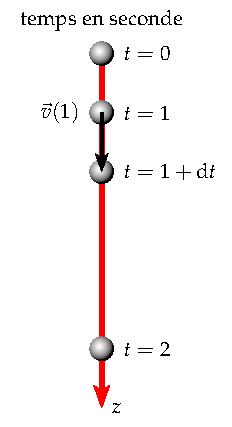
\includegraphics[scale=1]{.data/chute.pdf}
\end{center}
Remarquez ici que pour simplifier les calculs, l’axe des cotes est orienté vers le bas.
\begin{enumerate}
\item Quelle distance a parcouru la pierre au bout de 10s ?
\item Quelle est alors la vitesse moyenne pendant ces 10 premières
  secondes ?
\item Quelle distance a parcouru la pierre entre 15 et 20 secondes ?
\item Quelle est alors sa vitesse moyenne entre 15 et 20 secondes ?
\end{enumerate}
L’objectif est maintenant de trouver la vitesse INSTANTANEE à $t=1s$
\begin{enumerate}[resume]
\item Proposez une valeur approximative de cette vitesse instantanée ?
\item Proposez une méthode qui permet d’améliorer cette valeur.
\end{enumerate}
\end{exercice}

\begin{center}
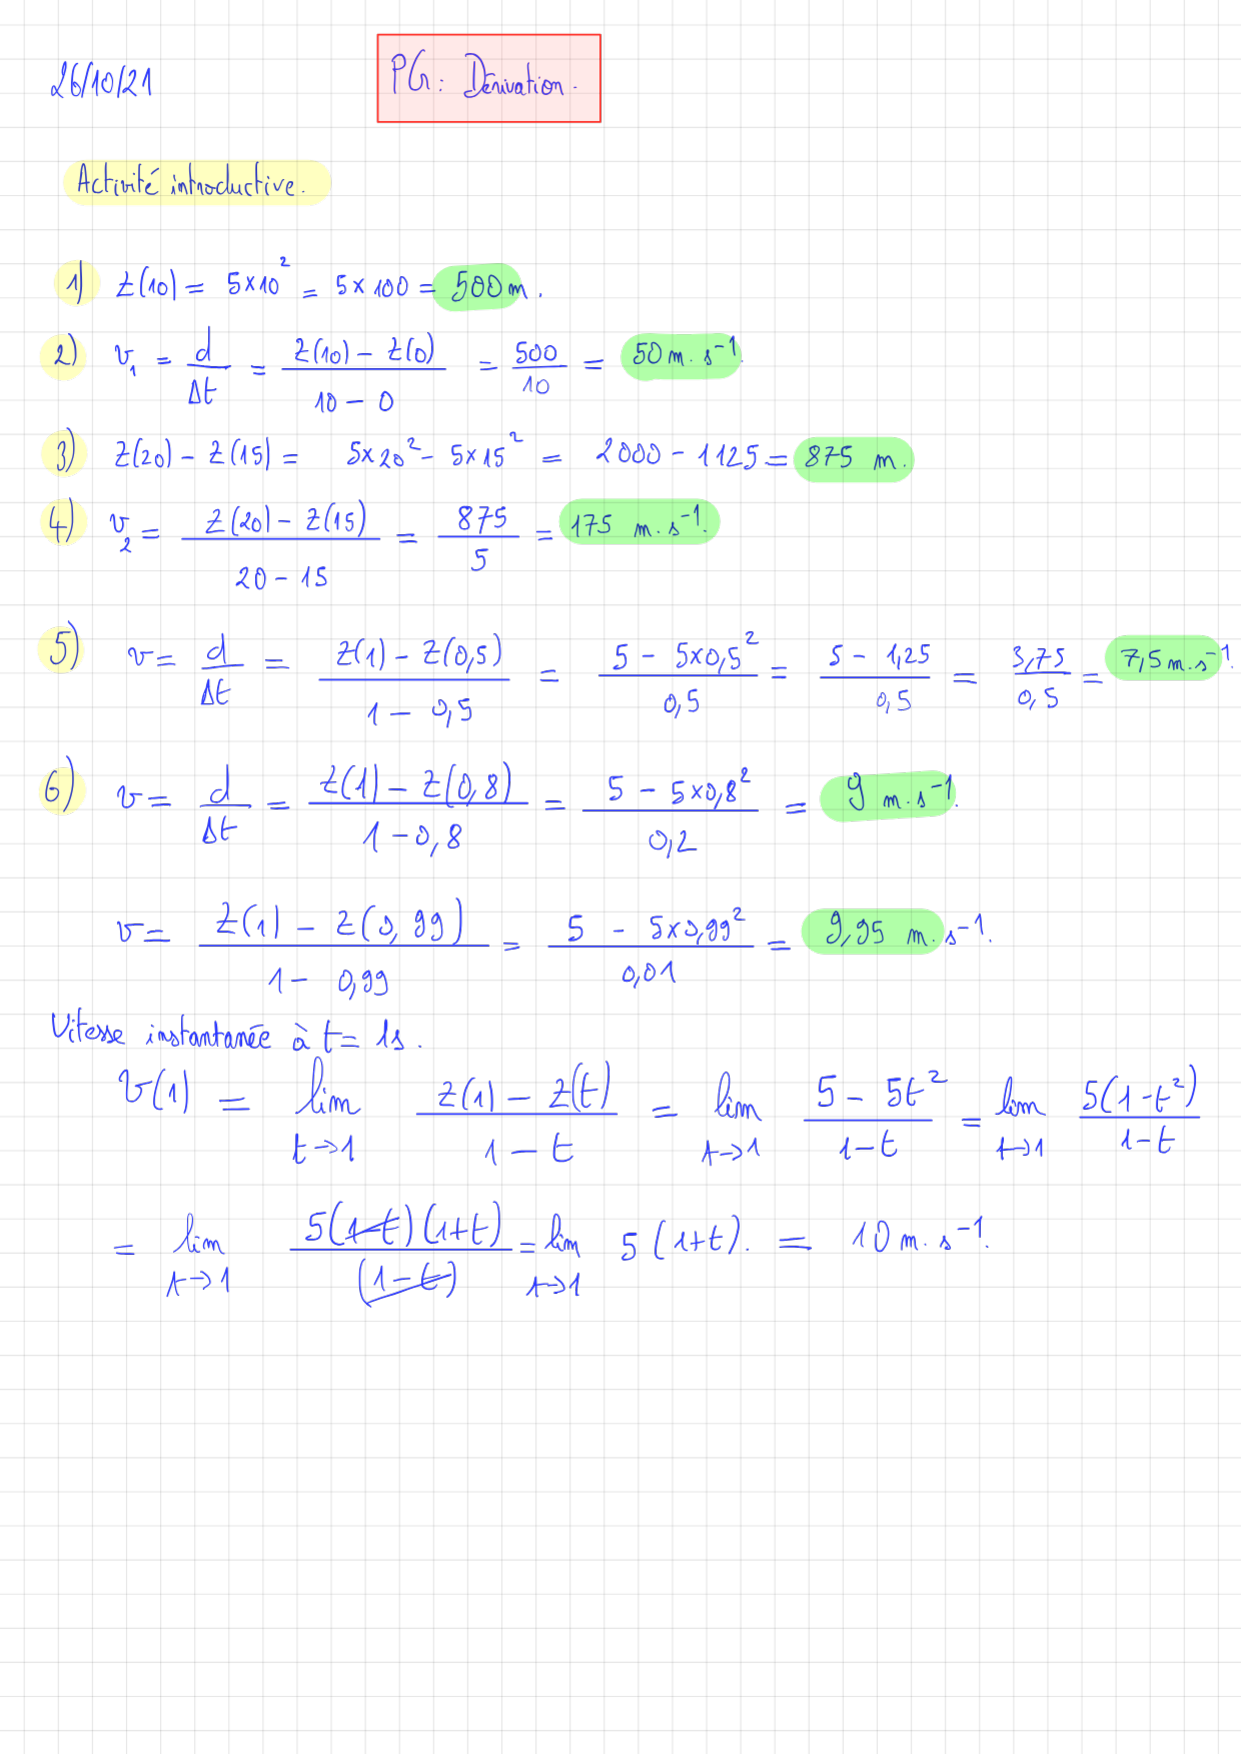
\includegraphics[scale=0.9]{.data/Derivation-corrigé.pdf}
\end{center}

\end{document}
%% Font size %%
\documentclass[11pt]{article}

%% Load the custom package
\usepackage{Mathdoc}

%% Numéro de séquence %% Titre de la séquence %%
\renewcommand{\centerhead}{Chap. 2 : Dérivation (Pentes et limites)}

%% Spacing commands %%
\renewcommand{\baselinestretch}{1}
\setlength{\parindent}{0pt}

\begin{document}
\phantom{0}
\vspace{-1.5cm}
\section{Pentes et fonctions affines}

\begin{multicols}{2}
\begin{exercice}
\textbf{Soit $\big(O ; \vec \imath,\vec \jmath\big)$ un repère orthogonal.  Déterminer, s'il existe et en l'expliquant, le coefficient directeur de la droite $(AB)$.}
\begin{enumerate}[itemsep=1em]
	\item \begin{minipage}[t]{\linewidth} Avec $A(0;-3)$ et $B(4;-3)$.  \end{minipage}
	\item \begin{minipage}[t]{\linewidth} Avec $A(4;4)$ et $B(4;2)$.  \end{minipage}
	\item \begin{minipage}[t]{\linewidth} Avec $A(-3;4)$ et $B(-1;-3)$.  \end{minipage}
	\item \begin{minipage}[t]{\linewidth} Avec $A(-3;-1)$ et $B(-1;-4)$.  \end{minipage}
	\item \begin{minipage}[t]{\linewidth} Avec $A(-3;-3)$ et $B(5;5)$.  \end{minipage}
\end{enumerate}
\end{exercice}

\begin{exercice}
\begin{enumerate}[itemsep=1em]
	\item Soit $f$ une fonction affine telle que $f(x)=ax+3$ et $f(1)=1$.\\    Donner la valeur de $a$.
    
	\item Soit $f$ une fonction affine telle que $f(x)=ax+1$ et $f(3)=-8$.\\    Donner la valeur de $a$.
    
	\item Soit $f$ une fonction affine telle que $f(x)=ax-2$ et $f(5)=-12$.\\      Donner la valeur de $a$.
    
	\item Soit $f$ une fonction affine telle que $f(x)=ax+4$ et $f(5)=12$.\\    Donner la valeur de $a$.
    
	\item Soit $f$ une fonction affine telle que $f(x)=ax-6$ et $f(5)=-13$.\\    Donner la valeur de $a$.
\end{enumerate}
\end{exercice}
\end{multicols}

\vspace{-1cm}
\section{Calculs de limites}

\begin{multicols}{2}
  \begin{exercice}
    \textbf{Calculer les limites en $0$ suivantes.}
    \begin{enumerate}
    \item \(\lim\limits_{x \to 0} (2x + 3)\)
    \item \(\lim\limits_{x \to 0} (x^2 + 5)\)
    \item \(\lim\limits_{x \to 0} \frac{1}{x + 1}\)
    \item \(\lim\limits_{x \to 0} (4x^3 - 2x)\)
    \item \(\lim\limits_{x \to 0} \sin(x)\)
    \item \(\lim\limits_{x \to 0} \frac{3x + 2}{x + 4}\)
    \item \(\lim\limits_{x \to 0} \cos(x)\)
    \item \(\lim\limits_{x \to 0} \frac{x}{x + 2}\)
    \item \(\lim\limits_{x \to 0} \frac{2x + 1}{x^2 + 1}\)
    \item \(\lim\limits_{x \to 0} \frac{5x^2}{x + 3}\)
    \end{enumerate}
  \end{exercice}

\begin{exercice}
  \textbf{Calculer les limites suivantes.}
  \begin{enumerate}
  \item \(\lim\limits_{x \to 2} (3x + 1)\)
  \item \(\lim\limits_{x \to -1} (x^2 + 4)\)
  \item \(\lim\limits_{x \to 3} \frac{2x + 5}{x + 1}\)
  \item \(\lim\limits_{x \to 4} (x^3 - 3x)\)
  \item \(\lim\limits_{x \to -2} \sin(x)\)
  \item \(\lim\limits_{x \to 1} \frac{4x^2 + 2x}{x + 3}\)
  \item \(\lim\limits_{x \to 0} \frac{x^2}{x + 2}\)
  \item \(\lim\limits_{x \to 5} \frac{3x - 2}{2x + 1}\)
  \item \(\lim\limits_{x \to -3} \frac{2x^2 + x}{x + 4}\)
  \item \(\lim\limits_{x \to 6} \frac{x^2 - 1}{x - 2}\)
  \end{enumerate}
\end{exercice}
\end{multicols}
\end{document}
%% Font size %%
\documentclass[11pt]{article}

%% Load the custom package
\usepackage{Mathdoc}

%% Numéro de séquence %% Titre de la séquence %%
\renewcommand{\centerhead}{}

%% Spacing commands %%
\renewcommand{\baselinestretch}{1}
\setlength{\parindent}{0pt}

\begin{document}


\begin{correction}[Exercice 1.1]
Calculer le nombre dérivé de $f(x)=x^2+x$ en $a=1$.\\
   \begin{tabular}{p{0.3cm}l!{=}l}
      &  $f'(a)$ & $\lim_{h\to0}\dfrac{f(a+h)-f(a)}{h}$ \\
   \end{tabular} \\

Or, $a=1$ donc :

   \begin{tabular}{p{0.3cm}l!{=}l}
      &  $f'(1)$ & $\lim\limits_{h\to0}\dfrac{f(1+h)-f(1)}{h}$ \\
   \end{tabular} \\

Calculons :\\
\begin{tabular}{p{0.3cm}l!{=}l}
      &  $f(1+h)$ & $(1+h)^2+1+h$\\
      &  & $1^2+2h+h^2+1+h$\\
      &  & $2+3h+h^2$\\
\end{tabular} \\


Calculons :\\
\begin{tabular}{p{0.3cm}l!{=}l}
      &  $f(1)$ & $(1)^2+1$\\
      &  & $2$\\
\end{tabular} \\

Donc :

   \begin{tabular}{p{0.3cm}l!{=}l}
      &  $f'(1)$ & $\lim\limits_{h\to0}\dfrac{2+3h+h^2-2}{h}$ \\
      &   & $\lim\limits_{h\to0}\dfrac{3h+h^2}{h}$ \\
      &   & $\lim\limits_{h\to0}3+h$ \\
      &  $f'(1)$ & $3$ \\
   \end{tabular} \\

\end{correction}

\newpage

\begin{exercice}
  
\end{exercice}

\end{document}
%% Font size %%
\documentclass[11pt]{article}

%% Load the custom package
\usepackage{Mathdoc}

%% Numéro de séquence %% Titre de la séquence %%
\renewcommand{\centerhead}{Chap. 2 : Dérivation (Problèmes de recherche)}

%% Spacing commands %%
\renewcommand{\baselinestretch}{1}
\setlength{\parindent}{0pt}

\begin{document}
\nopagebreak
\begin{exercice}[0][Expérimentations, et Calculs théoriques]
  \begin{center}
    \begin{tikzpicture}[ultra thick, scale=1]
      \begin{scope}
        \clip (-1, 0) rectangle (5, 7);
        \draw[gray!50!white, thin, xshift=-0.5cm, yshift=-0.5cm] (-1, -1) grid (6, 8);
        \draw[gray, thin] (-1, 0) grid (5, 7);
      \end{scope}
      \draw[-latex] (-1, 0) -- (5, 0);
      \draw[-latex] (0, 0) -- (0, 7);
      \foreach \x in {-1, 0, ..., 5} {
        \draw (\x, 0) node[below, fill=white, opacity=.7, text opacity=1]{$\x$};
      }
      \foreach \y in {1, 2, ..., 7} {
        \draw (0, \y) node[left, fill=white, opacity=.7, text opacity=1]{$\y$};
      }

      \draw[domain=-1:5,smooth,variable=\x,blue] plot ({\x},{\x*\x/4});

    %\draw[dashed] (2, 0) node[below]{$x$} -- (2, {2*2/4}) node{$\bullet$} -- (0, {2*2/4}) node[left]{$f\left( x \right)$};
    %\draw[dashed] (3, 0) node[below]{$x+h$} -- (3, {3*3/4}) node{$\bullet$} -- (0, {3*3/4}) node[left]{$f\left( x +h\right)$};
    %\draw[latex-latex] (2, -1) -- (3, -1) node[below, midway]{$h$};
    %\draw[dotted] (1, 0) -- (4, 3);
    \end{tikzpicture}
  \end{center}

  \begin{enumerate}
    \item On a tracé ci-dessus la courbe $\mathcal{C}_f$ de la fonction $f:x\mapsto \frac{x^2}{4}$.
      \begin{enumerate}
        \item Déterminer (par le calcul) l'équation de la tangente à $\mathcal{C}_f$ au point d'abscisse 2. On appelle $d$ la fonction affine correspondante.
        \item Tracer cette tangente.
        \item Calculer $f(x)-d(x)$ pour $x=4$, $x=3$, $x=2,5$, et $x=2,1$.
        \item Vers quelle valeur semble tendre $f\left( x \right)-d\left( x \right)$ lorsque $x$ tend vers 2 ?
      \end{enumerate}
    \item On cherche à résoudre l'équation différentielle :
      \[\left\{\begin{array}{l}
          2f\left( x \right)-xf'\left( x \right)=0\\
          f\left( 2 \right) = 1 \\
      \end{array}\right.\]
      Dans les questions \ref{q:euler:debut} à \ref{q:euler:fin}, on suppose que le tracé correspond \emph{exactement} au tracé de la courbe de la fonction $f$.
      \begin{enumerate}
        \item Isoler $f'\left( x \right)$ dans l'équation précédente.
        \item\label{q:euler:debut} Placer le point de coordonnées $\left( 2; f\left( 2 \right) \right)$.
        \item Calculer $f'\left( 2 \right)$, puis tracer le segment de la droite passant par le point de coordonnées $\left( 2; f\left( 2 \right) \right)$, et de coefficient directeur $f'(2)$, pour $x\in\left[ 2; 3 \right]$.
        \item\label{q:euler:fin} Même question, pour une abscisse de 3, puis de 4.
        \item Vérifier que la fonction $f:x\mapsto\frac{x^2}{4}$ est une solution de l'équation.
        \item Comparer la courbe tracée à cette question, et la courbe de la fonction $f$. Comment faire pour améliorer la précision du tracé ?
          % TODO Faire tracer cette courbe sur un autre graphique, et comparer ensuite les deux courbes
      \end{enumerate}
    \item \emph{Généralisation} Soit $f$ une fonction dérivable, et $a$ un réel de son ensemble de définition.
      On suppose que pour des valeurs de $h$ suffisament petites, $f\left( a+h \right)$ est exactement égale à l'image de $a+h$ par la tangente à $f$ en $a$.
      \begin{enumerate}
        \item Rappeler l'équation de la tangente à $f$ au point d'abscisse $a$.
        \item En déduire l'expression de $f\left( a+h \right)$ en fonction de $f\left( a \right)$, $f'\left( a \right)$ et $h$.
      \end{enumerate}
  \end{enumerate}
\end{exercice}


\end{document}
%% Font size %%
\documentclass[11pt]{article}

%% Load the custom package
\usepackage{Mathdoc}

%% Numéro de séquence %% Titre de la séquence %%
\renewcommand{\centerhead}{Extremum}

%% Spacing commands %%
\renewcommand{\baselinestretch}{1}
\setlength{\parindent}{0pt}

\begin{document}

\section{Recherche d'extremum}

\begin{exercice}[1][Formes cannoniques]
  \begin{enu}
\item On considère la fonction $f$ définie sur $\R$ par : $f(x)=5\left(x +\dfrac{9}{2}\right)^2 -\dfrac{441}{4}$.\\Déterminer l'extremum de la fonction $f$ ainsi que son image. 
	\item On considère la fonction $f$ définie sur $\R$ par : $f(x)=-3\left(x +5\right)^2 +68$.\\Déterminer l'extremum de la fonction $f$ ainsi que son image. 
	\item On considère la fonction $f$ définie sur $\R$ par : $f(x)=4\left(x +\dfrac{9}{2}\right)^2 -84$.\\Déterminer l'extremum de la fonction $f$ ainsi que son image. 
	\item On considère la fonction $f$ définie sur $\R$ par : $f(x)=-\left(x -5\right)^2 +22$.\\Déterminer l'extremum de la fonction $f$ ainsi que son image. 
  \end{enu}
\end{exercice}

\begin{exercice}[2][Formes développées]
  \begin{enu}
    \item On considère la fonction $f$ définie sur $\R$ par : $f(x)=5x^2+45x-9$.\\Déterminer l'extremum de la fonction $f$ ainsi que son image. 
	\item On considère la fonction $f$ définie sur $\R$ par : $f(x)=-3x^2-30x-7$.\\Déterminer l'extremum de la fonction $f$ ainsi que son image. 
	\item On considère la fonction $f$ définie sur $\R$ par : $f(x)=4x^2+36x-3$.\\Déterminer l'extremum de la fonction $f$ ainsi que son image. 
	\item On considère la fonction $f$ définie sur $\R$ par : $f(x)=-x^2+10x-3$.\\Déterminer l'extremum de la fonction $f$ ainsi que son image. 
  \end{enu}
\end{exercice}

\begin{exercice}[3][Formes factorisées]
  \begin{enu}
\item On considère la fonction $f$ définie sur $\R$ par : $f(x)=-3(x-5)(x-9)$.\\Déterminer l'extremum de la fonction $f$ ainsi que son image. 
	\item On considère la fonction $f$ définie sur $\R$ par : $f(x)=-2(x-1)(x-7)$.\\Déterminer l'extremum de la fonction $f$ ainsi que son image. 
	\item On considère la fonction $f$ définie sur $\R$ par : $f(x)=2(x-3)(x-5)$.\\Déterminer l'extremum de la fonction $f$ ainsi que son image. 
	\item On considère la fonction $f$ définie sur $\R$ par : $f(x)=3(x+1)(x-1)$.\\Déterminer l'extremum de la fonction $f$ ainsi que son image. 

  \end{enu}
\end{exercice}

\section{Lecture graphique}

\begin{exercice}[2][Répondre à ces questions par lecture graphique.]
  \begin{multicols}{2}
    \begin{enumerate}
    \item Quelles sont les coordonnées du sommet de la fonction
      polynomiale $\mathscr{f}$ du second degré représentée ci-dessous
      ?\\\begin{tikzpicture}[baseline,scale = 0.6]

        \tikzset{ point/.style={ thick, draw, cross out, inner
            sep=0pt, minimum width=5pt, minimum height=5pt, }, } \clip
        (-10,-1) rectangle (2,12);
    	
	\draw[color ={black},line width = 2,>=latex,->]
        (-10,0)--(1,0); \draw[color ={black},line width =
        2,>=latex,->] (0,0)--(0,10); \draw[color ={black},opacity =
        0.5] (-10,1)--(1,1); \draw[color ={black},opacity = 0.5]
        (-10,2)--(1,2); \draw[color ={black},opacity = 0.5]
        (-10,3)--(1,3); \draw[color ={black},opacity = 0.5]
        (-10,4)--(1,4); \draw[color ={black},opacity = 0.5]
        (-10,5)--(1,5); \draw[color ={black},opacity = 0.5]
        (-10,6)--(1,6); \draw[color ={black},opacity = 0.5]
        (-10,7)--(1,7); \draw[color ={black},opacity = 0.5]
        (-10,8)--(1,8); \draw[color ={black},opacity = 0.5]
        (-10,9)--(1,9); \draw[color ={black},opacity = 0.5]
        (-10,10)--(1,10); \draw[color ={black},opacity = 0.5]
        (1,0)--(1,10); \draw[color ={black},opacity = 0.5]
        (-1,0)--(-1,10); \draw[color ={black},opacity = 0.5]
        (-2,0)--(-2,10); \draw[color ={black},opacity = 0.5]
        (-3,0)--(-3,10); \draw[color ={black},opacity = 0.5]
        (-4,0)--(-4,10); \draw[color ={black},opacity = 0.5]
        (-5,0)--(-5,10); \draw[color ={black},opacity = 0.5]
        (-6,0)--(-6,10); \draw[color ={black},opacity = 0.5]
        (-7,0)--(-7,10); \draw[color ={black},opacity = 0.5]
        (-8,0)--(-8,10); \draw[color ={black},opacity = 0.5]
        (-9,0)--(-9,10); \draw[color ={black},opacity = 0.5]
        (-10,0)--(-10,10); \draw[color ={black},line width = 2]
        (-1,-0.2)--(-1,0.2); \draw[color ={black},line width = 2]
        (-2,-0.2)--(-2,0.2); \draw[color ={black},line width = 2]
        (-3,-0.2)--(-3,0.2); \draw[color ={black},line width = 2]
        (-4,-0.2)--(-4,0.2); \draw[color ={black},line width = 2]
        (-5,-0.2)--(-5,0.2); \draw[color ={black},line width = 2]
        (-6,-0.2)--(-6,0.2); \draw[color ={black},line width = 2]
        (-7,-0.2)--(-7,0.2); \draw[color ={black},line width = 2]
        (-8,-0.2)--(-8,0.2); \draw[color ={black},line width = 2]
        (-9,-0.2)--(-9,0.2); \draw[color ={black},line width = 2]
        (-0.2,1)--(0.2,1); \draw[color ={black},line width = 2]
        (-0.2,2)--(0.2,2); \draw[color ={black},line width = 2]
        (-0.2,3)--(0.2,3); \draw[color ={black},line width = 2]
        (-0.2,4)--(0.2,4); \draw[color ={black},line width = 2]
        (-0.2,5)--(0.2,5); \draw[color ={black},line width = 2]
        (-0.2,6)--(0.2,6); \draw[color ={black},line width = 2]
        (-0.2,7)--(0.2,7); \draw[color ={black},line width = 2]
        (-0.2,8)--(0.2,8); \draw[color ={black},line width = 2]
        (-0.2,9)--(0.2,9); \draw (-1,-0.4) node[anchor = center]
        {\scriptsize \color{black}{$-1$}}; \draw (-2,-0.4) node[anchor
        = center] {\scriptsize \color{black}{$-2$}}; \draw (-3,-0.4)
        node[anchor = center] {\scriptsize \color{black}{$-3$}}; \draw
        (-4,-0.4) node[anchor = center] {\scriptsize
          \color{black}{$-4$}}; \draw (-5,-0.4) node[anchor = center]
        {\scriptsize \color{black}{$-5$}}; \draw (-6,-0.4) node[anchor
        = center] {\scriptsize \color{black}{$-6$}}; \draw (-7,-0.4)
        node[anchor = center] {\scriptsize \color{black}{$-7$}}; \draw
        (-8,-0.4) node[anchor = center] {\scriptsize
          \color{black}{$-8$}}; \draw (-9,-0.4) node[anchor = center]
        {\scriptsize \color{black}{$-9$}}; \draw (-0.8,1.1)
        node[anchor = center] {\footnotesize \color{black}{$1$}};
        \draw (-0.8,2.1) node[anchor = center] {\footnotesize
          \color{black}{$2$}}; \draw (-0.8,3.1) node[anchor = center]
        {\footnotesize \color{black}{$3$}}; \draw (-0.8,4.1)
        node[anchor = center] {\footnotesize \color{black}{$4$}};
        \draw (-0.8,5.1) node[anchor = center] {\footnotesize
          \color{black}{$5$}}; \draw (-0.8,6.1) node[anchor = center]
        {\footnotesize \color{black}{$6$}}; \draw (-0.8,7.1)
        node[anchor = center] {\footnotesize \color{black}{$7$}};
        \draw (-0.8,8.1) node[anchor = center] {\footnotesize
          \color{black}{$8$}}; \draw (-0.8,9.1) node[anchor = center]
        {\footnotesize \color{black}{$9$}};
	
	\draw[color={blue},line width = 1.5]
        (-6.4,-0.76)--(-6.2,0.16)--(-6,1)--(-5.8,1.76)--(-5.6,2.44)--(-5.4,3.04)--(-5.2,3.56)--(-5,4)--(-4.8,4.36)--(-4.6,4.64)--(-4.4,4.84)--(-4.2,4.96)--(-4,5)--(-3.8,4.96)--(-3.6,4.84)--(-3.4,4.64)--(-3.2,4.36)--(-3,4)--(-2.8,3.56)--(-2.6,3.04)--(-2.4,2.44)--(-2.2,1.76)--(-2,1)--(-1.8,0.16)--(-1.6,-0.76);

      \end{tikzpicture}\\
    \item Quelles sont les coordonnées du sommet de la fonction
      polynomiale $\mathscr{g}$ du second degré représentée ci-dessous
      ?\\\begin{tikzpicture}[baseline,scale = 0.6]

        \tikzset{ point/.style={ thick, draw, cross out, inner
            sep=0pt, minimum width=5pt, minimum height=5pt, }, } \clip
        (-4,-3) rectangle (8,9);
    	
	\draw[color ={black},line width = 2,>=latex,->]
        (-10,0)--(7,0); \draw[color ={black},line width =
        2,>=latex,->] (0,-3)--(0,7); \draw[color ={black},opacity =
        0.5] (-10,1)--(7,1); \draw[color ={black},opacity = 0.5]
        (-10,2)--(7,2); \draw[color ={black},opacity = 0.5]
        (-10,3)--(7,3); \draw[color ={black},opacity = 0.5]
        (-10,4)--(7,4); \draw[color ={black},opacity = 0.5]
        (-10,5)--(7,5); \draw[color ={black},opacity = 0.5]
        (-10,6)--(7,6); \draw[color ={black},opacity = 0.5]
        (-10,7)--(7,7); \draw[color ={black},opacity = 0.5]
        (-10,-1)--(7,-1); \draw[color ={black},opacity = 0.5]
        (-10,-2)--(7,-2); \draw[color ={black},opacity = 0.5]
        (-10,-3)--(7,-3); \draw[color ={black},opacity = 0.5]
        (1,-3)--(1,7); \draw[color ={black},opacity = 0.5]
        (2,-3)--(2,7); \draw[color ={black},opacity = 0.5]
        (3,-3)--(3,7); \draw[color ={black},opacity = 0.5]
        (4,-3)--(4,7); \draw[color ={black},opacity = 0.5]
        (5,-3)--(5,7); \draw[color ={black},opacity = 0.5]
        (6,-3)--(6,7); \draw[color ={black},opacity = 0.5]
        (7,-3)--(7,7); \draw[color ={black},opacity = 0.5]
        (-1,-3)--(-1,7); \draw[color ={black},opacity = 0.5]
        (-2,-3)--(-2,7); \draw[color ={black},opacity = 0.5]
        (-3,-3)--(-3,7); \draw[color ={black},opacity = 0.5]
        (-4,-3)--(-4,7); \draw[color ={black},opacity = 0.5]
        (-5,-3)--(-5,7); \draw[color ={black},opacity = 0.5]
        (-6,-3)--(-6,7); \draw[color ={black},opacity = 0.5]
        (-7,-3)--(-7,7); \draw[color ={black},opacity = 0.5]
        (-8,-3)--(-8,7); \draw[color ={black},opacity = 0.5]
        (-9,-3)--(-9,7); \draw[color ={black},opacity = 0.5]
        (-10,-3)--(-10,7); \draw[color ={black},line width = 2]
        (1,-0.2)--(1,0.2); \draw[color ={black},line width = 2]
        (2,-0.2)--(2,0.2); \draw[color ={black},line width = 2]
        (3,-0.2)--(3,0.2); \draw[color ={black},line width = 2]
        (4,-0.2)--(4,0.2); \draw[color ={black},line width = 2]
        (5,-0.2)--(5,0.2); \draw[color ={black},line width = 2]
        (6,-0.2)--(6,0.2); \draw[color ={black},line width = 2]
        (-1,-0.2)--(-1,0.2); \draw[color ={black},line width = 2]
        (-2,-0.2)--(-2,0.2); \draw[color ={black},line width = 2]
        (-3,-0.2)--(-3,0.2); \draw[color ={black},line width = 2]
        (-4,-0.2)--(-4,0.2); \draw[color ={black},line width = 2]
        (-5,-0.2)--(-5,0.2); \draw[color ={black},line width = 2]
        (-6,-0.2)--(-6,0.2); \draw[color ={black},line width = 2]
        (-7,-0.2)--(-7,0.2); \draw[color ={black},line width = 2]
        (-8,-0.2)--(-8,0.2); \draw[color ={black},line width = 2]
        (-9,-0.2)--(-9,0.2); \draw[color ={black},line width = 2]
        (-0.2,1)--(0.2,1); \draw[color ={black},line width = 2]
        (-0.2,2)--(0.2,2); \draw[color ={black},line width = 2]
        (-0.2,3)--(0.2,3); \draw[color ={black},line width = 2]
        (-0.2,4)--(0.2,4); \draw[color ={black},line width = 2]
        (-0.2,5)--(0.2,5); \draw[color ={black},line width = 2]
        (-0.2,6)--(0.2,6); \draw[color ={black},line width = 2]
        (-0.2,-1)--(0.2,-1); \draw[color ={black},line width = 2]
        (-0.2,-2)--(0.2,-2); \draw (1,-0.4) node[anchor = center]
        {\scriptsize \color{black}{$1$}}; \draw (2,-0.4) node[anchor =
        center] {\scriptsize \color{black}{$2$}}; \draw (3,-0.4)
        node[anchor = center] {\scriptsize \color{black}{$3$}}; \draw
        (4,-0.4) node[anchor = center] {\scriptsize
          \color{black}{$4$}}; \draw (5,-0.4) node[anchor = center]
        {\scriptsize \color{black}{$5$}}; \draw (6,-0.4) node[anchor =
        center] {\scriptsize \color{black}{$6$}}; \draw (-1,-0.4)
        node[anchor = center] {\scriptsize \color{black}{$-1$}}; \draw
        (-2,-0.4) node[anchor = center] {\scriptsize
          \color{black}{$-2$}}; \draw (-3,-0.4) node[anchor = center]
        {\scriptsize \color{black}{$-3$}}; \draw (-4,-0.4) node[anchor
        = center] {\scriptsize \color{black}{$-4$}}; \draw (-5,-0.4)
        node[anchor = center] {\scriptsize \color{black}{$-5$}}; \draw
        (-6,-0.4) node[anchor = center] {\scriptsize
          \color{black}{$-6$}}; \draw (-7,-0.4) node[anchor = center]
        {\scriptsize \color{black}{$-7$}}; \draw (-8,-0.4) node[anchor
        = center] {\scriptsize \color{black}{$-8$}}; \draw (-9,-0.4)
        node[anchor = center] {\scriptsize \color{black}{$-9$}}; \draw
        (-0.8,1.1) node[anchor = center] {\footnotesize
          \color{black}{$1$}}; \draw (-0.8,2.1) node[anchor = center]
        {\footnotesize \color{black}{$2$}}; \draw (-0.8,3.1)
        node[anchor = center] {\footnotesize \color{black}{$3$}};
        \draw (-0.8,4.1) node[anchor = center] {\footnotesize
          \color{black}{$4$}}; \draw (-0.8,5.1) node[anchor = center]
        {\footnotesize \color{black}{$5$}}; \draw (-0.8,6.1)
        node[anchor = center] {\footnotesize \color{black}{$6$}};
        \draw (-0.8,-0.9) node[anchor = center] {\footnotesize
          \color{black}{$-1$}}; \draw (-0.8,-1.9) node[anchor =
        center] {\footnotesize \color{black}{$-2$}};
	
	\draw[color={blue},line width = 1.5]
        (-0.4,7.76)--(-0.2,6.84)--(0,6)--(0.2,5.24)--(0.4,4.56)--(0.6,3.96)--(0.8,3.44)--(1,3)--(1.2,2.64)--(1.4,2.36)--(1.6,2.16)--(1.8,2.04)--(2,2)--(2.2,2.04)--(2.4,2.16)--(2.6,2.36)--(2.8,2.64)--(3,3)--(3.2,3.44)--(3.4,3.96)--(3.6,4.56)--(3.8,5.24)--(4,6)--(4.2,6.84)--(4.4,7.76);

      \end{tikzpicture}\\
    \item Quelles sont les coordonnées du sommet de la fonction
      polynomiale $\mathscr{i}$ du second degré représentée ci-dessous
      ?\\\begin{tikzpicture}[baseline,scale = 0.6]

        \tikzset{ point/.style={ thick, draw, cross out, inner
            sep=0pt, minimum width=5pt, minimum height=5pt, }, } \clip
        (-10,-2) rectangle (2,10);
    	
	\draw[color ={black},line width = 2,>=latex,->]
        (-10,0)--(1,0); \draw[color ={black},line width =
        2,>=latex,->] (0,-2)--(0,8); \draw[color ={black},opacity =
        0.5] (-10,1)--(1,1); \draw[color ={black},opacity = 0.5]
        (-10,2)--(1,2); \draw[color ={black},opacity = 0.5]
        (-10,3)--(1,3); \draw[color ={black},opacity = 0.5]
        (-10,4)--(1,4); \draw[color ={black},opacity = 0.5]
        (-10,5)--(1,5); \draw[color ={black},opacity = 0.5]
        (-10,6)--(1,6); \draw[color ={black},opacity = 0.5]
        (-10,7)--(1,7); \draw[color ={black},opacity = 0.5]
        (-10,8)--(1,8); \draw[color ={black},opacity = 0.5]
        (-10,-1)--(1,-1); \draw[color ={black},opacity = 0.5]
        (-10,-2)--(1,-2); \draw[color ={black},opacity = 0.5]
        (1,-2)--(1,8); \draw[color ={black},opacity = 0.5]
        (-1,-2)--(-1,8); \draw[color ={black},opacity = 0.5]
        (-2,-2)--(-2,8); \draw[color ={black},opacity = 0.5]
        (-3,-2)--(-3,8); \draw[color ={black},opacity = 0.5]
        (-4,-2)--(-4,8); \draw[color ={black},opacity = 0.5]
        (-5,-2)--(-5,8); \draw[color ={black},opacity = 0.5]
        (-6,-2)--(-6,8); \draw[color ={black},opacity = 0.5]
        (-7,-2)--(-7,8); \draw[color ={black},opacity = 0.5]
        (-8,-2)--(-8,8); \draw[color ={black},opacity = 0.5]
        (-9,-2)--(-9,8); \draw[color ={black},opacity = 0.5]
        (-10,-2)--(-10,8); \draw[color ={black},line width = 2]
        (-1,-0.2)--(-1,0.2); \draw[color ={black},line width = 2]
        (-2,-0.2)--(-2,0.2); \draw[color ={black},line width = 2]
        (-3,-0.2)--(-3,0.2); \draw[color ={black},line width = 2]
        (-4,-0.2)--(-4,0.2); \draw[color ={black},line width = 2]
        (-5,-0.2)--(-5,0.2); \draw[color ={black},line width = 2]
        (-6,-0.2)--(-6,0.2); \draw[color ={black},line width = 2]
        (-7,-0.2)--(-7,0.2); \draw[color ={black},line width = 2]
        (-8,-0.2)--(-8,0.2); \draw[color ={black},line width = 2]
        (-9,-0.2)--(-9,0.2); \draw[color ={black},line width = 2]
        (-0.2,1)--(0.2,1); \draw[color ={black},line width = 2]
        (-0.2,2)--(0.2,2); \draw[color ={black},line width = 2]
        (-0.2,3)--(0.2,3); \draw[color ={black},line width = 2]
        (-0.2,4)--(0.2,4); \draw[color ={black},line width = 2]
        (-0.2,5)--(0.2,5); \draw[color ={black},line width = 2]
        (-0.2,6)--(0.2,6); \draw[color ={black},line width = 2]
        (-0.2,7)--(0.2,7); \draw[color ={black},line width = 2]
        (-0.2,-1)--(0.2,-1); \draw (-1,-0.4) node[anchor = center]
        {\scriptsize \color{black}{$-1$}}; \draw (-2,-0.4) node[anchor
        = center] {\scriptsize \color{black}{$-2$}}; \draw (-3,-0.4)
        node[anchor = center] {\scriptsize \color{black}{$-3$}}; \draw
        (-4,-0.4) node[anchor = center] {\scriptsize
          \color{black}{$-4$}}; \draw (-5,-0.4) node[anchor = center]
        {\scriptsize \color{black}{$-5$}}; \draw (-6,-0.4) node[anchor
        = center] {\scriptsize \color{black}{$-6$}}; \draw (-7,-0.4)
        node[anchor = center] {\scriptsize \color{black}{$-7$}}; \draw
        (-8,-0.4) node[anchor = center] {\scriptsize
          \color{black}{$-8$}}; \draw (-9,-0.4) node[anchor = center]
        {\scriptsize \color{black}{$-9$}}; \draw (-0.8,1.1)
        node[anchor = center] {\footnotesize \color{black}{$1$}};
        \draw (-0.8,2.1) node[anchor = center] {\footnotesize
          \color{black}{$2$}}; \draw (-0.8,3.1) node[anchor = center]
        {\footnotesize \color{black}{$3$}}; \draw (-0.8,4.1)
        node[anchor = center] {\footnotesize \color{black}{$4$}};
        \draw (-0.8,5.1) node[anchor = center] {\footnotesize
          \color{black}{$5$}}; \draw (-0.8,6.1) node[anchor = center]
        {\footnotesize \color{black}{$6$}}; \draw (-0.8,7.1)
        node[anchor = center] {\footnotesize \color{black}{$7$}};
        \draw (-0.8,-0.9) node[anchor = center] {\footnotesize
          \color{black}{$-1$}};
	
	\draw[color={blue},line width = 1.5]
        (-5.6,8.12)--(-5.4,6.92)--(-5.2,5.88)--(-5,5)--(-4.8,4.28)--(-4.6,3.72)--(-4.4,3.32)--(-4.2,3.08)--(-4,3)--(-3.8,3.08)--(-3.6,3.32)--(-3.4,3.72)--(-3.2,4.28)--(-3,5)--(-2.8,5.88)--(-2.6,6.92)--(-2.4,8.12);

      \end{tikzpicture}\\
    \item Quelles sont les coordonnées du sommet de la fonction
      polynomiale $\mathscr{j}$ du second degré représentée ci-dessous
      ?\\\begin{tikzpicture}[baseline,scale = 0.6]

        \tikzset{ point/.style={ thick, draw, cross out, inner
            sep=0pt, minimum width=5pt, minimum height=5pt, }, } \clip
        (-6,-10) rectangle (6,3);
    	
	\draw[color ={black},line width = 2,>=latex,->]
        (-10,0)--(5,0); \draw[color ={black},line width =
        2,>=latex,->] (0,-10)--(0,0); \draw[color ={black},opacity =
        0.5] (-10,-1)--(5,-1); \draw[color ={black},opacity = 0.5]
        (-10,-2)--(5,-2); \draw[color ={black},opacity = 0.5]
        (-10,-3)--(5,-3); \draw[color ={black},opacity = 0.5]
        (-10,-4)--(5,-4); \draw[color ={black},opacity = 0.5]
        (-10,-5)--(5,-5); \draw[color ={black},opacity = 0.5]
        (-10,-6)--(5,-6); \draw[color ={black},opacity = 0.5]
        (-10,-7)--(5,-7); \draw[color ={black},opacity = 0.5]
        (-10,-8)--(5,-8); \draw[color ={black},opacity = 0.5]
        (-10,-9)--(5,-9); \draw[color ={black},opacity = 0.5]
        (-10,-10)--(5,-10); \draw[color ={black},opacity = 0.5]
        (1,-10)--(1,0); \draw[color ={black},opacity = 0.5]
        (2,-10)--(2,0); \draw[color ={black},opacity = 0.5]
        (3,-10)--(3,0); \draw[color ={black},opacity = 0.5]
        (4,-10)--(4,0); \draw[color ={black},opacity = 0.5]
        (5,-10)--(5,0); \draw[color ={black},opacity = 0.5]
        (-1,-10)--(-1,0); \draw[color ={black},opacity = 0.5]
        (-2,-10)--(-2,0); \draw[color ={black},opacity = 0.5]
        (-3,-10)--(-3,0); \draw[color ={black},opacity = 0.5]
        (-4,-10)--(-4,0); \draw[color ={black},opacity = 0.5]
        (-5,-10)--(-5,0); \draw[color ={black},opacity = 0.5]
        (-6,-10)--(-6,0); \draw[color ={black},opacity = 0.5]
        (-7,-10)--(-7,0); \draw[color ={black},opacity = 0.5]
        (-8,-10)--(-8,0); \draw[color ={black},opacity = 0.5]
        (-9,-10)--(-9,0); \draw[color ={black},opacity = 0.5]
        (-10,-10)--(-10,0); \draw[color ={black},line width = 2]
        (1,-0.2)--(1,0.2); \draw[color ={black},line width = 2]
        (2,-0.2)--(2,0.2); \draw[color ={black},line width = 2]
        (3,-0.2)--(3,0.2); \draw[color ={black},line width = 2]
        (4,-0.2)--(4,0.2); \draw[color ={black},line width = 2]
        (-1,-0.2)--(-1,0.2); \draw[color ={black},line width = 2]
        (-2,-0.2)--(-2,0.2); \draw[color ={black},line width = 2]
        (-3,-0.2)--(-3,0.2); \draw[color ={black},line width = 2]
        (-4,-0.2)--(-4,0.2); \draw[color ={black},line width = 2]
        (-5,-0.2)--(-5,0.2); \draw[color ={black},line width = 2]
        (-6,-0.2)--(-6,0.2); \draw[color ={black},line width = 2]
        (-7,-0.2)--(-7,0.2); \draw[color ={black},line width = 2]
        (-8,-0.2)--(-8,0.2); \draw[color ={black},line width = 2]
        (-9,-0.2)--(-9,0.2); \draw[color ={black},line width = 2]
        (-0.2,-1)--(0.2,-1); \draw[color ={black},line width = 2]
        (-0.2,-2)--(0.2,-2); \draw[color ={black},line width = 2]
        (-0.2,-3)--(0.2,-3); \draw[color ={black},line width = 2]
        (-0.2,-4)--(0.2,-4); \draw[color ={black},line width = 2]
        (-0.2,-5)--(0.2,-5); \draw[color ={black},line width = 2]
        (-0.2,-6)--(0.2,-6); \draw[color ={black},line width = 2]
        (-0.2,-7)--(0.2,-7); \draw[color ={black},line width = 2]
        (-0.2,-8)--(0.2,-8); \draw[color ={black},line width = 2]
        (-0.2,-9)--(0.2,-9); \draw (1,-0.4) node[anchor = center]
        {\scriptsize \color{black}{$1$}}; \draw (2,-0.4) node[anchor =
        center] {\scriptsize \color{black}{$2$}}; \draw (3,-0.4)
        node[anchor = center] {\scriptsize \color{black}{$3$}}; \draw
        (4,-0.4) node[anchor = center] {\scriptsize
          \color{black}{$4$}}; \draw (-1,-0.4) node[anchor = center]
        {\scriptsize \color{black}{$-1$}}; \draw (-2,-0.4) node[anchor
        = center] {\scriptsize \color{black}{$-2$}}; \draw (-3,-0.4)
        node[anchor = center] {\scriptsize \color{black}{$-3$}}; \draw
        (-4,-0.4) node[anchor = center] {\scriptsize
          \color{black}{$-4$}}; \draw (-5,-0.4) node[anchor = center]
        {\scriptsize \color{black}{$-5$}}; \draw (-6,-0.4) node[anchor
        = center] {\scriptsize \color{black}{$-6$}}; \draw (-7,-0.4)
        node[anchor = center] {\scriptsize \color{black}{$-7$}}; \draw
        (-8,-0.4) node[anchor = center] {\scriptsize
          \color{black}{$-8$}}; \draw (-9,-0.4) node[anchor = center]
        {\scriptsize \color{black}{$-9$}}; \draw (-0.8,-0.9)
        node[anchor = center] {\footnotesize \color{black}{$-1$}};
        \draw (-0.8,-1.9) node[anchor = center] {\footnotesize
          \color{black}{$-2$}}; \draw (-0.8,-2.9) node[anchor =
        center] {\footnotesize \color{black}{$-3$}}; \draw (-0.8,-3.9)
        node[anchor = center] {\footnotesize \color{black}{$-4$}};
        \draw (-0.8,-4.9) node[anchor = center] {\footnotesize
          \color{black}{$-5$}}; \draw (-0.8,-5.9) node[anchor =
        center] {\footnotesize \color{black}{$-6$}}; \draw (-0.8,-6.9)
        node[anchor = center] {\footnotesize \color{black}{$-7$}};
        \draw (-0.8,-7.9) node[anchor = center] {\footnotesize
          \color{black}{$-8$}}; \draw (-0.8,-8.9) node[anchor =
        center] {\footnotesize \color{black}{$-9$}};
	
	\draw[color={blue},line width = 1.5]
        (-1.6,-10.12)--(-1.4,-8.92)--(-1.2,-7.88)--(-1,-7)--(-0.8,-6.28)--(-0.6,-5.72)--(-0.4,-5.32)--(-0.2,-5.08)--(0,-5)--(0.2,-5.08)--(0.4,-5.32)--(0.6,-5.72)--(0.8,-6.28)--(1,-7)--(1.2,-7.88)--(1.4,-8.92)--(1.6,-10.12);

      \end{tikzpicture}
 \end{enumerate}
\end{multicols}
\end{exercice}


\section{Tableaux de variations}

\begin{exercice}[0][Exercice Corrigé.]
 On considère la fonction $f$ définie sur $\R$ par :
 $f(x)=4x^2-20x-6$.\\
 Dresser le tableau de  variations de la fonction $f$ sur
 $\R$. \\
 \textbf{Correction.}
 \begin{enumerate}[label=(\arabic*)]
 \item On reconnaît la forme développée d'une fonction polynôme du
   second degré $ax^2+bx+c$ avec $a=4$, $b=-20$ et $c=-6$.
 \item Comme $a > 0$, la fonction est d'abord décroissante puis croissante.
 \item Le changement de variation s'opère en
   $\alpha=-\dfrac{b}{2a}=\dfrac{-(-20)}{2\times
     4}=\dfrac{5}{2}$. 
 \item De plus, $f\left(\dfrac{5}{2}\right)=4 \times \left(\dfrac{5}{2}
   \right)^2 -20 \times \dfrac{5}{2} -6 = -31$.
 \item On en déduit le tableau de variations de $f$ sur $\R$ :
   \begin{center}
     \begin{tikzpicture}[baseline, scale=0.75]
       \tkzTabInit[lgt=3,deltacl=0.8,espcl=4.5]{ $x$ / 1.5, $f(x)$ /
         3}{ $-\infty$, $\dfrac{5}{2}$, $+\infty$} \tkzTabVar{ +/ ,
         -/$-31$, +/ }
     \end{tikzpicture}
   \end{center}
 \end{enumerate}
\end{exercice}

\begin{exercice}[2][Tableaux de variations sur $\R$]
  \begin{enu}
    \item On considère la fonction $f$ définie sur $\R$ par : $f(x)=-x^2-7x+4$.\\Dresser le tableau de  variations de la fonction $f$ sur $\R$.
	\item On considère la fonction $f$ définie sur $\R$ par : $f(x)=3x(x+2)$.\\Dresser le tableau de  variations de la fonction $f$ sur $\R$.
	\item On considère la fonction $f$ définie sur $\R$ par : $f(x)=5\left(x -\dfrac{3}{2}\right)^2 -\dfrac{41}{4}$.\\Dresser le tableau de  variations de la fonction $f$ sur $\R$.
	\item On considère la fonction $f$ définie sur $\R$ par : $f(x)=-5\left(x -5\right)^2 +119$.\\Dresser le tableau de  variations de la fonction $f$ sur $\R$.
	\item On considère la fonction $f$ définie sur $\R$ par : $f(x)=3(x+1)(x-5)$.\\Dresser le tableau de  variations de la fonction $f$ sur $\R$.
  \end{enu}
\end{exercice}

\newpage

\phantom{0}
\vspace{-1cm}

\begin{exercice}[2][Tableaux de variations sur un intervalle borné]
  \begin{enu}
	\item On considère la fonction $f$ définie sur $[3\,;\,10]$ par : $f(x)=-x^2-7x+4$.\\Dresser le tableau de  variations de la fonction $f$ sur $[3\,;\,10]$.
	\item On considère la fonction $f$ définie sur $[1\,;\,6]$ par : $f(x)=3x(x+2)$.\\Dresser le tableau de  variations de la fonction $f$ sur $[1\,;\,6]$.
	\item On considère la fonction $f$ définie sur $[5\,;\,10]$ par : $f(x)=5\left(x -\dfrac{3}{2}\right)^2 -\dfrac{41}{4}$.\\Dresser le tableau de  variations de la fonction $f$ sur $[5\,;\,10]$.
	\item On considère la fonction $f$ définie sur $[0\,;\,7]$ par : $f(x)=-5\left(x -5\right)^2 +119$.\\Dresser le tableau de  variations de la fonction $f$ sur $[0\,;\,7]$.
	\item On considère la fonction $f$ définie sur $[4\,;\,6]$ par : $f(x)=3(x+1)(x-5)$.\\Dresser le tableau de  variations de la fonction $f$ sur $[4\,;\,6]$.
  \end{enu}
\end{exercice}

\vspace{-.5cm}

\begin{exercice}[3][Étude d'une fonction polynomiale]
  Soit $f(x)=\left(x +3\right)^2 -19$ un polynôme du second degré définie sur $\R$.
  \begin{enumerate}
  \item Déterminer le sens de variation de $f$ sur $\R$.
  \item Déterminer l'extremum de la fonction $f$ puis calculer son
    image.
  \item Dresser le tableau de variation de la fonction $f$ sur $\R$.
  \item Dans un repère orthonormé direct, représenter la fonction $f$ sur l'intervalle
    $[-7\,;\,1]$
  \end{enumerate}
\end{exercice}

\vspace{-.5cm}

\begin{exercice}[3][Étude d'une fonction polynomiale]
  Soit $f(x)=2x^2-2x-10$ un polynôme du second degré définie sur $\R$.
  \begin{enumerate}
  \item Déterminer le sens de variation de $f$ sur $\R$.
  \item Déterminer l'extremum de la fonction $f$ puis calculer son
    image.
  \item Dresser le tableau de variation de la fonction $f$ sur $\R$.
  \item Dans un repère orthonormé direct, représenter la fonction $f$ sur l'intervalle
    $[-4\,;\,4]$
  \end{enumerate}
\end{exercice}

\nopagebreak

\begin{exercice}[4][Étude d'une fonction polynomiale]
  Soit $f(x)=-2(x+1)(x-1)$ un polynôme du second degré définie sur $\R$.
  \begin{enumerate}
  \item Déterminer le sens de variation de $f$ sur $\R$.
  \item Déterminer l'extremum de la fonction $f$ puis calculer son
    image.
  \item Dresser le tableau de variation de la fonction $f$ sur $\R$.
  \item Dans un repère orthonormé direct, représenter la fonction $f$ sur l'intervalle
    $[-4\,;\,4]$
  \end{enumerate}
\end{exercice}


\end{document}

%%% Local Variables:
%%% mode: LaTeX
%%% TeX-master: t
%%% End:
%% Font size %%
\documentclass[11pt]{article}

%% Load the custom package
\usepackage{Mathdoc}

%% Numéro de séquence %% Titre de la séquence %%
\renewcommand{\centerhead}{Sens de variations}

%% Spacing commands %%
\renewcommand{\baselinestretch}{1}
\setlength{\parindent}{0pt}

\begin{document}

\phantom{0}
\vspace{-1cm}
\section{Sens de variation d'une fonction affine}

\vspace{-.5cm}
\begin{exercice}[0][Exerice corrigé.]
 Déterminer le sens de variation de la fonction $v$ définie sur
 $\mathbb R$ par : $v(x)=2-5x$.
 \begin{multicols}{2}
   \textbf{Correction.} \\
   On reconnaît que $v$ est une fonction affine, de la forme $v(x)=ax+b$, avec $a=-5~$ et $b=2$. \\
   On sait qu'une fonction affine est monotone sur $\mathbb{R}$.\\
   Son sens de variation dépend du signe de $a$.\\Comme $a=-5<0$ , la
   fonction $v$ est strictement décroissante sur $\mathbb{R}$.\\On
   peut synthétiser cela dans un tableau de
   variations :
   
   \begin{center}
     \begin{tikzpicture}[baseline, scale=0.5]
       \tkzTabInit[lgt=3,deltacl=0.8,espcl=5]{ $x$ / 2, $v(x)$ / 3}{
         $-\infty$, $+\infty$} \tkzTabVar{ +/, -/}
     \end{tikzpicture}
   \end{center}
 \end{multicols}
\end{exercice}

\vspace{-.5cm}
\begin{exercice}[1][Sens de variations simples.]
\begin{enu}
	\item Déterminer le sens de variation de la fonction $v$ définie sur $\mathbb R$ par : $v(x)=-5+4x$.
	\item Dresser le tableau de variations de la fonction $w$ définie sur $[5\,;\,10]$ par : $w(x)=-7+5x$.
	\item Déterminer le sens de variation de la fonction $u$ définie sur $\mathbb R$ par : $u(x)=\dfrac{7-7x}{8}$.
	\item Déterminer le sens de variation de la fonction $g$ définie sur $\mathbb R$ par : $g(x)=10+10x$.
	\item Dresser le tableau de variations de la fonction $h$ définie sur $[-7\,;\,-6]$ par : $h(x)=x+4$.
\end{enu}
\end{exercice}

\vspace{-1cm}
\section{Sens de variation d'une fonction polynome du second degré}

\vspace{-.5cm}
\begin{exercice}[0][Exerice corrigé.]
On considère la fonction $f$ définie sur $\mathbb{R}$ par :
$f(x)=4x^2-40x+8$. \\
Étudier les variations de $f$ sur $\R$.\\
\textbf{Correction.}\\
$f(x)=4x^2-40x+8$ est de la forme $ax^2+bx+c$, avec $a=4$, $b=-40$ et
$c=8$. \\
On a : $a < 0$ donc $f(x)$ est décroissante puis croissante. 
\end{exercice}

\begin{exercice}[2][Étude global du sens de variation]
  \begin{multicols}{2}
    \begin{enu}
      \item On considère la fonction $f$ définie sur $\mathbb{R}$ par
        : $f(x)=-2(x-3)(x-5)$.\\Étudier les variations de $f$ sur
        $\R$.
      \item On considère la fonction $f$ définie sur $\mathbb{R}$ par
        : $f(x)=-2x^2-10x-6$.\\Étudier les variations de $f$ sur $\R$.
      \item On considère la fonction $f$ définie sur $\mathbb{R}$ par
        :
        $f(x)=-3\left(x -\dfrac{5}{2}\right)^2
        +\dfrac{103}{4}$.\\Étudier les variations de $f$ sur $\R$.
      \item On considère la fonction $f$ définie sur $\mathbb{R}$ par
        : $f(x)=-3(x-2)(x-6)$.\\Étudier les variations de $f$ sur
        $\R$.
      \item On considère la fonction $f$ définie sur $\mathbb{R}$ par
        : $f(x)=3x^2+18x-3$.\\Étudier les variations de $f$ sur $\R$.
      \item On considère la fonction $f$ définie sur $\mathbb{R}$ par
        : $f(x)=-5\left(x -3\right)^2 +47$.\\Étudier les variations de
        $f$ sur $\R$.
    \end{enu}
  \end{multicols}
\end{exercice}

\newpage

\section{Lecture graphique}

\begin{exercice}[2][Répondre à ces questions par lecture graphique.]
  \begin{multicols}{2}
    \begin{enumerate}[itemsep=1em]
    \item Quel est le signe du coefficient dominant de la fonction
      polynomiale $\mathscr{f}$ du second degré représentée ci-dessous
      ?\\\begin{tikzpicture}[baseline,scale = 0.6]

        \tikzset{ point/.style={ thick, draw, cross out, inner
            sep=0pt, minimum width=5pt, minimum height=5pt, }, } \clip
        (3,-1) rectangle (12,4);
    	
	\draw[color ={black},line width = 2,>=latex,->]
        (-10,0)--(11,0); \draw[color ={black},line width =
        2,>=latex,->] (0,-1)--(0,2); \draw[color ={black},opacity =
        0.5] (1,-1)--(1,2); \draw[color ={black},opacity = 0.5]
        (2,-1)--(2,2); \draw[color ={black},opacity = 0.5]
        (3,-1)--(3,2); \draw[color ={black},opacity = 0.5]
        (4,-1)--(4,2); \draw[color ={black},opacity = 0.5]
        (5,-1)--(5,2); \draw[color ={black},opacity = 0.5]
        (6,-1)--(6,2); \draw[color ={black},opacity = 0.5]
        (7,-1)--(7,2); \draw[color ={black},opacity = 0.5]
        (8,-1)--(8,2); \draw[color ={black},opacity = 0.5]
        (9,-1)--(9,2); \draw[color ={black},opacity = 0.5]
        (10,-1)--(10,2); \draw[color ={black},opacity = 0.5]
        (11,-1)--(11,2); \draw[color ={black},opacity = 0.5]
        (-1,-1)--(-1,2); \draw[color ={black},opacity = 0.5]
        (-2,-1)--(-2,2); \draw[color ={black},opacity = 0.5]
        (-3,-1)--(-3,2); \draw[color ={black},opacity = 0.5]
        (-4,-1)--(-4,2); \draw[color ={black},opacity = 0.5]
        (-5,-1)--(-5,2); \draw[color ={black},opacity = 0.5]
        (-6,-1)--(-6,2); \draw[color ={black},opacity = 0.5]
        (-7,-1)--(-7,2); \draw[color ={black},opacity = 0.5]
        (-8,-1)--(-8,2); \draw[color ={black},opacity = 0.5]
        (-9,-1)--(-9,2); \draw[color ={black},opacity = 0.5]
        (-10,-1)--(-10,2); \draw[color ={black},line width = 2]
        (1,-0.2)--(1,0.2); \draw[color ={black},line width = 2]
        (2,-0.2)--(2,0.2); \draw[color ={black},line width = 2]
        (3,-0.2)--(3,0.2); \draw[color ={black},line width = 2]
        (4,-0.2)--(4,0.2); \draw[color ={black},line width = 2]
        (5,-0.2)--(5,0.2); \draw[color ={black},line width = 2]
        (6,-0.2)--(6,0.2); \draw[color ={black},line width = 2]
        (7,-0.2)--(7,0.2); \draw[color ={black},line width = 2]
        (8,-0.2)--(8,0.2); \draw[color ={black},line width = 2]
        (9,-0.2)--(9,0.2); \draw[color ={black},line width = 2]
        (10,-0.2)--(10,0.2); \draw[color ={black},line width = 2]
        (-1,-0.2)--(-1,0.2); \draw[color ={black},line width = 2]
        (-2,-0.2)--(-2,0.2); \draw[color ={black},line width = 2]
        (-3,-0.2)--(-3,0.2); \draw[color ={black},line width = 2]
        (-4,-0.2)--(-4,0.2); \draw[color ={black},line width = 2]
        (-5,-0.2)--(-5,0.2); \draw[color ={black},line width = 2]
        (-6,-0.2)--(-6,0.2); \draw[color ={black},line width = 2]
        (-7,-0.2)--(-7,0.2); \draw[color ={black},line width = 2]
        (-8,-0.2)--(-8,0.2); \draw[color ={black},line width = 2]
        (-9,-0.2)--(-9,0.2); \draw[color ={black},line width = 2]
        (-0.2,1)--(0.2,1); \draw (1,-0.4) node[anchor = center]
        {\scriptsize \color{black}{$1$}}; \draw (2,-0.4) node[anchor =
        center] {\scriptsize \color{black}{$2$}}; \draw (3,-0.4)
        node[anchor = center] {\scriptsize \color{black}{$3$}}; \draw
        (4,-0.4) node[anchor = center] {\scriptsize
          \color{black}{$4$}}; \draw (5,-0.4) node[anchor = center]
        {\scriptsize \color{black}{$5$}}; \draw (6,-0.4) node[anchor =
        center] {\scriptsize \color{black}{$6$}}; \draw (7,-0.4)
        node[anchor = center] {\scriptsize \color{black}{$7$}}; \draw
        (8,-0.4) node[anchor = center] {\scriptsize
          \color{black}{$8$}}; \draw (9,-0.4) node[anchor = center]
        {\scriptsize \color{black}{$9$}}; \draw (10,-0.4) node[anchor
        = center] {\scriptsize \color{black}{$10$}}; \draw (-1,-0.4)
        node[anchor = center] {\scriptsize \color{black}{$-1$}}; \draw
        (-2,-0.4) node[anchor = center] {\scriptsize
          \color{black}{$-2$}}; \draw (-3,-0.4) node[anchor = center]
        {\scriptsize \color{black}{$-3$}}; \draw (-4,-0.4) node[anchor
        = center] {\scriptsize \color{black}{$-4$}}; \draw (-5,-0.4)
        node[anchor = center] {\scriptsize \color{black}{$-5$}}; \draw
        (-6,-0.4) node[anchor = center] {\scriptsize
          \color{black}{$-6$}}; \draw (-7,-0.4) node[anchor = center]
        {\scriptsize \color{black}{$-7$}}; \draw (-8,-0.4) node[anchor
        = center] {\scriptsize \color{black}{$-8$}}; \draw (-9,-0.4)
        node[anchor = center] {\scriptsize \color{black}{$-9$}}; \draw
        (-0.8,1.1) node[anchor = center] {\footnotesize
          \color{black}{$10$}};
	
	\draw[color={blue},line width = 1.5]
        (4,2)--(4.2,1.73)--(4.4,1.47)--(4.6,1.23)--(4.8,1.01)--(5,0.8)--(5.2,0.61)--(5.4,0.43)--(5.6,0.27)--(5.8,0.13)--(6,0)--(6.2,-0.11)--(6.4,-0.21)--(6.6,-0.29)--(6.8,-0.35)--(7,-0.4)--(7.2,-0.43)--(7.4,-0.45)--(7.6,-0.45)--(7.8,-0.43)--(8,-0.4)--(8.2,-0.35)--(8.4,-0.29)--(8.6,-0.21)--(8.8,-0.11)--(9,0)--(9.2,0.13)--(9.4,0.27)--(9.6,0.43)--(9.8,0.61)--(10,0.8)--(10.2,1.01)--(10.4,1.23)--(10.6,1.47)--(10.8,1.73)--(11,2);

      \end{tikzpicture}\\
    \item Quel est le signe du coefficient dominant de la fonction
      polynomiale $\mathscr{g}$ du second degré représentée ci-dessous
      ?\\\begin{tikzpicture}[baseline,scale = 0.6]

        \tikzset{ point/.style={ thick, draw, cross out, inner
            sep=0pt, minimum width=5pt, minimum height=5pt, }, } \clip
        (4,-2.5) rectangle (13,7);
    	
	\draw[color ={black},line width = 2,>=latex,->]
        (-10,0)--(12,0); \draw[color ={black},line width =
        2,>=latex,->] (0,-3)--(0,5); \draw[color ={black},opacity =
        0.5] (-10,2)--(12,2); \draw[color ={black},opacity = 0.5]
        (-10,4)--(12,4); \draw[color ={black},opacity = 0.5]
        (-10,-2)--(12,-2); \draw[color ={black},opacity = 0.5]
        (1,-3)--(1,5); \draw[color ={black},opacity = 0.5]
        (2,-3)--(2,5); \draw[color ={black},opacity = 0.5]
        (3,-3)--(3,5); \draw[color ={black},opacity = 0.5]
        (4,-3)--(4,5); \draw[color ={black},opacity = 0.5]
        (5,-3)--(5,5); \draw[color ={black},opacity = 0.5]
        (6,-3)--(6,5); \draw[color ={black},opacity = 0.5]
        (7,-3)--(7,5); \draw[color ={black},opacity = 0.5]
        (8,-3)--(8,5); \draw[color ={black},opacity = 0.5]
        (9,-3)--(9,5); \draw[color ={black},opacity = 0.5]
        (10,-3)--(10,5); \draw[color ={black},opacity = 0.5]
        (11,-3)--(11,5); \draw[color ={black},opacity = 0.5]
        (12,-3)--(12,5); \draw[color ={black},opacity = 0.5]
        (-1,-3)--(-1,5); \draw[color ={black},opacity = 0.5]
        (-2,-3)--(-2,5); \draw[color ={black},opacity = 0.5]
        (-3,-3)--(-3,5); \draw[color ={black},opacity = 0.5]
        (-4,-3)--(-4,5); \draw[color ={black},opacity = 0.5]
        (-5,-3)--(-5,5); \draw[color ={black},opacity = 0.5]
        (-6,-3)--(-6,5); \draw[color ={black},opacity = 0.5]
        (-7,-3)--(-7,5); \draw[color ={black},opacity = 0.5]
        (-8,-3)--(-8,5); \draw[color ={black},opacity = 0.5]
        (-9,-3)--(-9,5); \draw[color ={black},opacity = 0.5]
        (-10,-3)--(-10,5); \draw[color ={black},line width = 2]
        (1,-0.2)--(1,0.2); \draw[color ={black},line width = 2]
        (2,-0.2)--(2,0.2); \draw[color ={black},line width = 2]
        (3,-0.2)--(3,0.2); \draw[color ={black},line width = 2]
        (4,-0.2)--(4,0.2); \draw[color ={black},line width = 2]
        (5,-0.2)--(5,0.2); \draw[color ={black},line width = 2]
        (6,-0.2)--(6,0.2); \draw[color ={black},line width = 2]
        (7,-0.2)--(7,0.2); \draw[color ={black},line width = 2]
        (8,-0.2)--(8,0.2); \draw[color ={black},line width = 2]
        (9,-0.2)--(9,0.2); \draw[color ={black},line width = 2]
        (10,-0.2)--(10,0.2); \draw[color ={black},line width = 2]
        (11,-0.2)--(11,0.2); \draw[color ={black},line width = 2]
        (-1,-0.2)--(-1,0.2); \draw[color ={black},line width = 2]
        (-2,-0.2)--(-2,0.2); \draw[color ={black},line width = 2]
        (-3,-0.2)--(-3,0.2); \draw[color ={black},line width = 2]
        (-4,-0.2)--(-4,0.2); \draw[color ={black},line width = 2]
        (-5,-0.2)--(-5,0.2); \draw[color ={black},line width = 2]
        (-6,-0.2)--(-6,0.2); \draw[color ={black},line width = 2]
        (-7,-0.2)--(-7,0.2); \draw[color ={black},line width = 2]
        (-8,-0.2)--(-8,0.2); \draw[color ={black},line width = 2]
        (-9,-0.2)--(-9,0.2); \draw[color ={black},line width = 2]
        (-0.2,1)--(0.2,1); \draw[color ={black},line width = 2]
        (-0.2,2)--(0.2,2); \draw[color ={black},line width = 2]
        (-0.2,3)--(0.2,3); \draw[color ={black},line width = 2]
        (-0.2,4)--(0.2,4); \draw[color ={black},line width = 2]
        (-0.2,-1)--(0.2,-1); \draw[color ={black},line width = 2]
        (-0.2,-2)--(0.2,-2); \draw (1,-0.4) node[anchor = center]
        {\scriptsize \color{black}{$1$}}; \draw (2,-0.4) node[anchor =
        center] {\scriptsize \color{black}{$2$}}; \draw (3,-0.4)
        node[anchor = center] {\scriptsize \color{black}{$3$}}; \draw
        (4,-0.4) node[anchor = center] {\scriptsize
          \color{black}{$4$}}; \draw (5,-0.4) node[anchor = center]
        {\scriptsize \color{black}{$5$}}; \draw (6,-0.4) node[anchor =
        center] {\scriptsize \color{black}{$6$}}; \draw (7,-0.4)
        node[anchor = center] {\scriptsize \color{black}{$7$}}; \draw
        (8,-0.4) node[anchor = center] {\scriptsize
          \color{black}{$8$}}; \draw (9,-0.4) node[anchor = center]
        {\scriptsize \color{black}{$9$}}; \draw (10,-0.4) node[anchor
        = center] {\scriptsize \color{black}{$10$}}; \draw (11,-0.4)
        node[anchor = center] {\scriptsize \color{black}{$11$}}; \draw
        (-1,-0.4) node[anchor = center] {\scriptsize
          \color{black}{$-1$}}; \draw (-2,-0.4) node[anchor = center]
        {\scriptsize \color{black}{$-2$}}; \draw (-3,-0.4) node[anchor
        = center] {\scriptsize \color{black}{$-3$}}; \draw (-4,-0.4)
        node[anchor = center] {\scriptsize \color{black}{$-4$}}; \draw
        (-5,-0.4) node[anchor = center] {\scriptsize
          \color{black}{$-5$}}; \draw (-6,-0.4) node[anchor = center]
        {\scriptsize \color{black}{$-6$}}; \draw (-7,-0.4) node[anchor
        = center] {\scriptsize \color{black}{$-7$}}; \draw (-8,-0.4)
        node[anchor = center] {\scriptsize \color{black}{$-8$}}; \draw
        (-9,-0.4) node[anchor = center] {\scriptsize
          \color{black}{$-9$}}; \draw (-0.8,1.1) node[anchor = center]
        {\footnotesize \color{black}{$2$}}; \draw (-0.8,2.1)
        node[anchor = center] {\footnotesize \color{black}{$4$}};
        \draw (-0.8,3.1) node[anchor = center] {\footnotesize
          \color{black}{$6$}}; \draw (-0.8,4.1) node[anchor = center]
        {\footnotesize \color{black}{$8$}}; \draw (-0.8,-0.9)
        node[anchor = center] {\footnotesize \color{black}{$-2$}};
        \draw (-0.8,-1.9) node[anchor = center] {\footnotesize
          \color{black}{$-4$}};
	
	\draw[color={blue},line width = 1.5]
        (5,5)--(5.2,4.32)--(5.4,3.68)--(5.6,3.08)--(5.8,2.52)--(6,2)--(6.2,1.52)--(6.4,1.08)--(6.6,0.68)--(6.8,0.32)--(7,0)--(7.2,-0.28)--(7.4,-0.52)--(7.6,-0.72)--(7.8,-0.88)--(8,-1)--(8.2,-1.08)--(8.4,-1.12)--(8.6,-1.12)--(8.8,-1.08)--(9,-1)--(9.2,-0.88)--(9.4,-0.72)--(9.6,-0.52)--(9.8,-0.28)--(10,0)--(10.2,0.32)--(10.4,0.68)--(10.6,1.08)--(10.8,1.52)--(11,2)--(11.2,2.52)--(11.4,3.08)--(11.6,3.68)--(11.8,4.32)--(12,5);

      \end{tikzpicture}\\
    \item Quel est le signe du coefficient dominant de la fonction
      polynomiale $\mathscr{h}$ du second degré représentée ci-dessous
      ?\\\begin{tikzpicture}[baseline,scale = 0.6]

        \tikzset{ point/.style={ thick, draw, cross out, inner
            sep=0pt, minimum width=5pt, minimum height=5pt, }, } \clip
        (-7,-1.5) rectangle (6,3.8);
    	
	\draw[color ={black},line width = 2,>=latex,->]
        (-10,0)--(5,0); \draw[color ={black},line width =
        2,>=latex,->] (0,-2)--(0,2); \draw[color ={black},opacity =
        0.5] (1,-2)--(1,2); \draw[color ={black},opacity = 0.5]
        (2,-2)--(2,2); \draw[color ={black},opacity = 0.5]
        (3,-2)--(3,2); \draw[color ={black},opacity = 0.5]
        (4,-2)--(4,2); \draw[color ={black},opacity = 0.5]
        (5,-2)--(5,2); \draw[color ={black},opacity = 0.5]
        (-1,-2)--(-1,2); \draw[color ={black},opacity = 0.5]
        (-2,-2)--(-2,2); \draw[color ={black},opacity = 0.5]
        (-3,-2)--(-3,2); \draw[color ={black},opacity = 0.5]
        (-4,-2)--(-4,2); \draw[color ={black},opacity = 0.5]
        (-5,-2)--(-5,2); \draw[color ={black},opacity = 0.5]
        (-6,-2)--(-6,2); \draw[color ={black},opacity = 0.5]
        (-7,-2)--(-7,2); \draw[color ={black},opacity = 0.5]
        (-8,-2)--(-8,2); \draw[color ={black},opacity = 0.5]
        (-9,-2)--(-9,2); \draw[color ={black},opacity = 0.5]
        (-10,-2)--(-10,2); \draw[color ={black},line width = 2]
        (1,-0.2)--(1,0.2); \draw[color ={black},line width = 2]
        (2,-0.2)--(2,0.2); \draw[color ={black},line width = 2]
        (3,-0.2)--(3,0.2); \draw[color ={black},line width = 2]
        (4,-0.2)--(4,0.2); \draw[color ={black},line width = 2]
        (-1,-0.2)--(-1,0.2); \draw[color ={black},line width = 2]
        (-2,-0.2)--(-2,0.2); \draw[color ={black},line width = 2]
        (-3,-0.2)--(-3,0.2); \draw[color ={black},line width = 2]
        (-4,-0.2)--(-4,0.2); \draw[color ={black},line width = 2]
        (-5,-0.2)--(-5,0.2); \draw[color ={black},line width = 2]
        (-6,-0.2)--(-6,0.2); \draw[color ={black},line width = 2]
        (-7,-0.2)--(-7,0.2); \draw[color ={black},line width = 2]
        (-8,-0.2)--(-8,0.2); \draw[color ={black},line width = 2]
        (-9,-0.2)--(-9,0.2); \draw[color ={black},line width = 2]
        (-0.2,1)--(0.2,1); \draw[color ={black},line width = 2]
        (-0.2,-1)--(0.2,-1); \draw (1,-0.4) node[anchor = center]
        {\scriptsize \color{black}{$1$}}; \draw (2,-0.4) node[anchor =
        center] {\scriptsize \color{black}{$2$}}; \draw (3,-0.4)
        node[anchor = center] {\scriptsize \color{black}{$3$}}; \draw
        (4,-0.4) node[anchor = center] {\scriptsize
          \color{black}{$4$}}; \draw (-1,-0.4) node[anchor = center]
        {\scriptsize \color{black}{$-1$}}; \draw (-2,-0.4) node[anchor
        = center] {\scriptsize \color{black}{$-2$}}; \draw (-3,-0.4)
        node[anchor = center] {\scriptsize \color{black}{$-3$}}; \draw
        (-4,-0.4) node[anchor = center] {\scriptsize
          \color{black}{$-4$}}; \draw (-5,-0.4) node[anchor = center]
        {\scriptsize \color{black}{$-5$}}; \draw (-6,-0.4) node[anchor
        = center] {\scriptsize \color{black}{$-6$}}; \draw (-7,-0.4)
        node[anchor = center] {\scriptsize \color{black}{$-7$}}; \draw
        (-8,-0.4) node[anchor = center] {\scriptsize
          \color{black}{$-8$}}; \draw (-9,-0.4) node[anchor = center]
        {\scriptsize \color{black}{$-9$}}; \draw (-0.8,1.1)
        node[anchor = center] {\footnotesize \color{black}{$10$}};
        \draw (-0.8,-0.9) node[anchor = center] {\footnotesize
          \color{black}{$-10$}};
	
	\draw[color={blue},line width = 1.5]
        (-6,1.8)--(-5.8,1.58)--(-5.6,1.38)--(-5.4,1.18)--(-5.2,0.98)--(-5,0.8)--(-4.8,0.62)--(-4.6,0.46)--(-4.4,0.3)--(-4.2,0.14)--(-4,0)--(-3.8,-0.14)--(-3.6,-0.26)--(-3.4,-0.38)--(-3.2,-0.5)--(-3,-0.6)--(-2.8,-0.7)--(-2.6,-0.78)--(-2.4,-0.86)--(-2.2,-0.94)--(-2,-1)--(-1.8,-1.06)--(-1.6,-1.1)--(-1.4,-1.14)--(-1.2,-1.18)--(-1,-1.2)--(-0.8,-1.22)--(-0.6,-1.22)--(-0.4,-1.22)--(-0.2,-1.22)--(0,-1.2)--(0.2,-1.18)--(0.4,-1.14)--(0.6,-1.1)--(0.8,-1.06)--(1,-1)--(1.2,-0.94)--(1.4,-0.86)--(1.6,-0.78)--(1.8,-0.7)--(2,-0.6)--(2.2,-0.5)--(2.4,-0.38)--(2.6,-0.26)--(2.8,-0.14)--(3,0)--(3.2,0.14)--(3.4,0.3)--(3.6,0.46)--(3.8,0.62)--(4,0.8)--(4.2,0.98)--(4.4,1.18)--(4.6,1.38)--(4.8,1.58)--(5,1.8);

      \end{tikzpicture}\\
    \item Quel est le signe du coefficient dominant de la fonction
      polynomiale $\mathscr{i}$ du second degré représentée ci-dessous
      ?\\\begin{tikzpicture}[baseline,scale = 0.4]

        \tikzset{ point/.style={ thick, draw, cross out, inner
            sep=0pt, minimum width=5pt, minimum height=5pt, }, } \clip
        (-11,-1.5) rectangle (8,4.25);
    	
	\draw[color ={black},line width = 2,>=latex,->]
        (-10,0)--(7,0); \draw[color ={black},line width =
        2,>=latex,->] (0,-2)--(0,3); \draw[color ={black},opacity =
        0.5] (1,-2)--(1,3); \draw[color ={black},opacity = 0.5]
        (2,-2)--(2,3); \draw[color ={black},opacity = 0.5]
        (3,-2)--(3,3); \draw[color ={black},opacity = 0.5]
        (4,-2)--(4,3); \draw[color ={black},opacity = 0.5]
        (5,-2)--(5,3); \draw[color ={black},opacity = 0.5]
        (6,-2)--(6,3); \draw[color ={black},opacity = 0.5]
        (7,-2)--(7,3); \draw[color ={black},opacity = 0.5]
        (-1,-2)--(-1,3); \draw[color ={black},opacity = 0.5]
        (-2,-2)--(-2,3); \draw[color ={black},opacity = 0.5]
        (-3,-2)--(-3,3); \draw[color ={black},opacity = 0.5]
        (-4,-2)--(-4,3); \draw[color ={black},opacity = 0.5]
        (-5,-2)--(-5,3); \draw[color ={black},opacity = 0.5]
        (-6,-2)--(-6,3); \draw[color ={black},opacity = 0.5]
        (-7,-2)--(-7,3); \draw[color ={black},opacity = 0.5]
        (-8,-2)--(-8,3); \draw[color ={black},opacity = 0.5]
        (-9,-2)--(-9,3); \draw[color ={black},opacity = 0.5]
        (-10,-2)--(-10,3); \draw[color ={black},line width = 2]
        (1,-0.2)--(1,0.2); \draw[color ={black},line width = 2]
        (2,-0.2)--(2,0.2); \draw[color ={black},line width = 2]
        (3,-0.2)--(3,0.2); \draw[color ={black},line width = 2]
        (4,-0.2)--(4,0.2); \draw[color ={black},line width = 2]
        (5,-0.2)--(5,0.2); \draw[color ={black},line width = 2]
        (6,-0.2)--(6,0.2); \draw[color ={black},line width = 2]
        (-1,-0.2)--(-1,0.2); \draw[color ={black},line width = 2]
        (-2,-0.2)--(-2,0.2); \draw[color ={black},line width = 2]
        (-3,-0.2)--(-3,0.2); \draw[color ={black},line width = 2]
        (-4,-0.2)--(-4,0.2); \draw[color ={black},line width = 2]
        (-5,-0.2)--(-5,0.2); \draw[color ={black},line width = 2]
        (-6,-0.2)--(-6,0.2); \draw[color ={black},line width = 2]
        (-7,-0.2)--(-7,0.2); \draw[color ={black},line width = 2]
        (-8,-0.2)--(-8,0.2); \draw[color ={black},line width = 2]
        (-9,-0.2)--(-9,0.2); \draw[color ={black},line width = 2]
        (-0.2,1)--(0.2,1); \draw[color ={black},line width = 2]
        (-0.2,2)--(0.2,2); \draw[color ={black},line width = 2]
        (-0.2,-1)--(0.2,-1); \draw (1,-0.4) node[anchor = center]
        {\scriptsize \color{black}{$1$}}; \draw (2,-0.4) node[anchor =
        center] {\scriptsize \color{black}{$2$}}; \draw (3,-0.4)
        node[anchor = center] {\scriptsize \color{black}{$3$}}; \draw
        (4,-0.4) node[anchor = center] {\scriptsize
          \color{black}{$4$}}; \draw (5,-0.4) node[anchor = center]
        {\scriptsize \color{black}{$5$}}; \draw (6,-0.4) node[anchor =
        center] {\scriptsize \color{black}{$6$}}; \draw (-1,-0.4)
        node[anchor = center] {\scriptsize \color{black}{$-1$}}; \draw
        (-2,-0.4) node[anchor = center] {\scriptsize
          \color{black}{$-2$}}; \draw (-3,-0.4) node[anchor = center]
        {\scriptsize \color{black}{$-3$}}; \draw (-4,-0.4) node[anchor
        = center] {\scriptsize \color{black}{$-4$}}; \draw (-5,-0.4)
        node[anchor = center] {\scriptsize \color{black}{$-5$}}; \draw
        (-6,-0.4) node[anchor = center] {\scriptsize
          \color{black}{$-6$}}; \draw (-7,-0.4) node[anchor = center]
        {\scriptsize \color{black}{$-7$}}; \draw (-8,-0.4) node[anchor
        = center] {\scriptsize \color{black}{$-8$}}; \draw (-9,-0.4)
        node[anchor = center] {\scriptsize \color{black}{$-9$}}; \draw
        (-0.8,1.1) node[anchor = center] {\footnotesize
          \color{black}{$20$}}; \draw (-0.8,2.1) node[anchor = center]
        {\footnotesize \color{black}{$40$}}; \draw (-0.8,-0.9)
        node[anchor = center] {\footnotesize \color{black}{$-20$}};
	
	\draw[color={blue},line width = 1.5]
        (-10,-1.5)--(-9.8,-1.33)--(-9.6,-1.17)--(-9.4,-1.01)--(-9.2,-0.85)--(-9,-0.7)--(-8.8,-0.55)--(-8.6,-0.41)--(-8.4,-0.27)--(-8.2,-0.13)--(-8,0)--(-7.8,0.13)--(-7.6,0.25)--(-7.4,0.37)--(-7.2,0.49)--(-7,0.6)--(-6.8,0.71)--(-6.6,0.81)--(-6.4,0.91)--(-6.2,1.01)--(-6,1.1)--(-5.8,1.19)--(-5.6,1.27)--(-5.4,1.35)--(-5.2,1.43)--(-5,1.5)--(-4.8,1.57)--(-4.6,1.63)--(-4.4,1.69)--(-4.2,1.75)--(-4,1.8)--(-3.8,1.85)--(-3.6,1.89)--(-3.4,1.93)--(-3.2,1.97)--(-3,2)--(-2.8,2.03)--(-2.6,2.05)--(-2.4,2.07)--(-2.2,2.09)--(-2,2.1)--(-1.8,2.11)--(-1.6,2.11)--(-1.4,2.11)--(-1.2,2.11)--(-1,2.1)--(-0.8,2.09)--(-0.6,2.07)--(-0.4,2.05)--(-0.2,2.03)--(0,2)--(0.2,1.97)--(0.4,1.93)--(0.6,1.89)--(0.8,1.85)--(1,1.8)--(1.2,1.75)--(1.4,1.69)--(1.6,1.63)--(1.8,1.57)--(2,1.5)--(2.2,1.43)--(2.4,1.35)--(2.6,1.27)--(2.8,1.19)--(3,1.1)--(3.2,1.01)--(3.4,0.91)--(3.6,0.81)--(3.8,0.71)--(4,0.6)--(4.2,0.49)--(4.4,0.37)--(4.6,0.25)--(4.8,0.13)--(5,0)--(5.2,-0.13)--(5.4,-0.27)--(5.6,-0.41)--(5.8,-0.55)--(6,-0.7)--(6.2,-0.85)--(6.4,-1.01)--(6.6,-1.17)--(6.8,-1.33)--(7,-1.5);

      \end{tikzpicture}
\item Quel est le signe du coefficient dominant de la fonction polynomiale $\mathscr{f}$ du second degré représentée ci-dessous ?\\\begin{tikzpicture}[baseline,scale = 0.6]

    \tikzset{
      point/.style={
        thick,
        draw,
        cross out,
        inner sep=0pt,
        minimum width=5pt,
        minimum height=5pt,
      },
    }
    \clip (-11,-2.4) rectangle (-1,3);
    	
	\draw[color ={black},line width = 2,>=latex,->] (-10,0)--(-2,0);
	\draw[color ={black},line width = 2,>=latex,->] (0,-3)--(0,1);
	\draw[color ={black},opacity = 0.5] (-1,-3)--(-1,1);
	\draw[color ={black},opacity = 0.5] (-2,-3)--(-2,1);
	\draw[color ={black},opacity = 0.5] (-3,-3)--(-3,1);
	\draw[color ={black},opacity = 0.5] (-4,-3)--(-4,1);
	\draw[color ={black},opacity = 0.5] (-5,-3)--(-5,1);
	\draw[color ={black},opacity = 0.5] (-6,-3)--(-6,1);
	\draw[color ={black},opacity = 0.5] (-7,-3)--(-7,1);
	\draw[color ={black},opacity = 0.5] (-8,-3)--(-8,1);
	\draw[color ={black},opacity = 0.5] (-9,-3)--(-9,1);
	\draw[color ={black},opacity = 0.5] (-10,-3)--(-10,1);
	\draw[color ={black},line width = 2] (-1,-0.2)--(-1,0.2);
	\draw[color ={black},line width = 2] (-2,-0.2)--(-2,0.2);
	\draw[color ={black},line width = 2] (-3,-0.2)--(-3,0.2);
	\draw[color ={black},line width = 2] (-4,-0.2)--(-4,0.2);
	\draw[color ={black},line width = 2] (-5,-0.2)--(-5,0.2);
	\draw[color ={black},line width = 2] (-6,-0.2)--(-6,0.2);
	\draw[color ={black},line width = 2] (-7,-0.2)--(-7,0.2);
	\draw[color ={black},line width = 2] (-8,-0.2)--(-8,0.2);
	\draw[color ={black},line width = 2] (-9,-0.2)--(-9,0.2);
	\draw[color ={black},line width = 2] (-0.2,-1)--(0.2,-1);
	\draw[color ={black},line width = 2] (-0.2,-2)--(0.2,-2);
	\draw (-2,-0.4) node[anchor = center] {\scriptsize \color{black}{$-2$}};
	\draw (-3,-0.4) node[anchor = center] {\scriptsize \color{black}{$-3$}};
	\draw (-4,-0.4) node[anchor = center] {\scriptsize \color{black}{$-4$}};
	\draw (-5,-0.4) node[anchor = center] {\scriptsize \color{black}{$-5$}};
	\draw (-6,-0.4) node[anchor = center] {\scriptsize \color{black}{$-6$}};
	\draw (-7,-0.4) node[anchor = center] {\scriptsize \color{black}{$-7$}};
	\draw (-8,-0.4) node[anchor = center] {\scriptsize \color{black}{$-8$}};
	\draw (-9,-0.4) node[anchor = center] {\scriptsize \color{black}{$-9$}};
	\draw (-0.8,-0.9) node[anchor = center] {\footnotesize \color{black}{$-10$}};
	\draw (-0.8,-1.9) node[anchor = center] {\footnotesize \color{black}{$-20$}};
	
	\draw[color={blue},line width = 1.5] (-10,-2.4)--(-9.8,-2.09)--(-9.6,-1.79)--(-9.4,-1.51)--(-9.2,-1.25)--(-9,-1)--(-8.8,-0.77)--(-8.6,-0.55)--(-8.4,-0.35)--(-8.2,-0.17)--(-8,0)--(-7.8,0.15)--(-7.6,0.29)--(-7.4,0.41)--(-7.2,0.51)--(-7,0.6)--(-6.8,0.67)--(-6.6,0.73)--(-6.4,0.77)--(-6.2,0.79)--(-6,0.8)--(-5.8,0.79)--(-5.6,0.77)--(-5.4,0.73)--(-5.2,0.67)--(-5,0.6)--(-4.8,0.51)--(-4.6,0.41)--(-4.4,0.29)--(-4.2,0.15)--(-4,0)--(-3.8,-0.17)--(-3.6,-0.35)--(-3.4,-0.55)--(-3.2,-0.77)--(-3,-1)--(-2.8,-1.25)--(-2.6,-1.51)--(-2.4,-1.79)--(-2.2,-2.09)--(-2,-2.4);

\end{tikzpicture}\\
	\item Quel est le signe du coefficient dominant de la fonction polynomiale $\mathscr{g}$ du second degré représentée ci-dessous ?\\\begin{tikzpicture}[baseline,scale = 0.6]

    \tikzset{
      point/.style={
        thick,
        draw,
        cross out,
        inner sep=0pt,
        minimum width=5pt,
        minimum height=5pt,
      },
    }
    \clip (-11,-1.4) rectangle (0,3);
    	
	\draw[color ={black},line width = 2,>=latex,->] (-10,0)--(-1,0);
	\draw[color ={black},line width = 2,>=latex,->] (0,-2)--(0,1);
	\draw[color ={black},opacity = 0.5] (-1,-2)--(-1,1);
	\draw[color ={black},opacity = 0.5] (-2,-2)--(-2,1);
	\draw[color ={black},opacity = 0.5] (-3,-2)--(-3,1);
	\draw[color ={black},opacity = 0.5] (-4,-2)--(-4,1);
	\draw[color ={black},opacity = 0.5] (-5,-2)--(-5,1);
	\draw[color ={black},opacity = 0.5] (-6,-2)--(-6,1);
	\draw[color ={black},opacity = 0.5] (-7,-2)--(-7,1);
	\draw[color ={black},opacity = 0.5] (-8,-2)--(-8,1);
	\draw[color ={black},opacity = 0.5] (-9,-2)--(-9,1);
	\draw[color ={black},opacity = 0.5] (-10,-2)--(-10,1);
	\draw[color ={black},line width = 2] (-1,-0.2)--(-1,0.2);
	\draw[color ={black},line width = 2] (-2,-0.2)--(-2,0.2);
	\draw[color ={black},line width = 2] (-3,-0.2)--(-3,0.2);
	\draw[color ={black},line width = 2] (-4,-0.2)--(-4,0.2);
	\draw[color ={black},line width = 2] (-5,-0.2)--(-5,0.2);
	\draw[color ={black},line width = 2] (-6,-0.2)--(-6,0.2);
	\draw[color ={black},line width = 2] (-7,-0.2)--(-7,0.2);
	\draw[color ={black},line width = 2] (-8,-0.2)--(-8,0.2);
	\draw[color ={black},line width = 2] (-9,-0.2)--(-9,0.2);
	\draw[color ={black},line width = 2] (-0.2,-1)--(0.2,-1);
	\draw (-1,-0.4) node[anchor = center] {\scriptsize \color{black}{$-1$}};
	\draw (-2,-0.4) node[anchor = center] {\scriptsize \color{black}{$-2$}};
	\draw (-3,-0.4) node[anchor = center] {\scriptsize \color{black}{$-3$}};
	\draw (-4,-0.4) node[anchor = center] {\scriptsize \color{black}{$-4$}};
	\draw (-5,-0.4) node[anchor = center] {\scriptsize \color{black}{$-5$}};
	\draw (-6,-0.4) node[anchor = center] {\scriptsize \color{black}{$-6$}};
	\draw (-7,-0.4) node[anchor = center] {\scriptsize \color{black}{$-7$}};
	\draw (-8,-0.4) node[anchor = center] {\scriptsize \color{black}{$-8$}};
	\draw (-9,-0.4) node[anchor = center] {\scriptsize \color{black}{$-9$}};
	\draw (-0.8,-0.9) node[anchor = center] {\footnotesize \color{black}{$-10$}};
	
	\draw[color={blue},line width = 1.5] (-10,-1.4)--(-9.8,-1.22)--(-9.6,-1.06)--(-9.4,-0.9)--(-9.2,-0.74)--(-9,-0.6)--(-8.8,-0.46)--(-8.6,-0.34)--(-8.4,-0.22)--(-8.2,-0.1)--(-8,0)--(-7.8,0.1)--(-7.6,0.18)--(-7.4,0.26)--(-7.2,0.34)--(-7,0.4)--(-6.8,0.46)--(-6.6,0.5)--(-6.4,0.54)--(-6.2,0.58)--(-6,0.6)--(-5.8,0.62)--(-5.6,0.62)--(-5.4,0.62)--(-5.2,0.62)--(-5,0.6)--(-4.8,0.58)--(-4.6,0.54)--(-4.4,0.5)--(-4.2,0.46)--(-4,0.4)--(-3.8,0.34)--(-3.6,0.26)--(-3.4,0.18)--(-3.2,0.1)--(-3,0)--(-2.8,-0.1)--(-2.6,-0.22)--(-2.4,-0.34)--(-2.2,-0.46)--(-2,-0.6)--(-1.8,-0.74)--(-1.6,-0.9)--(-1.4,-1.06)--(-1.2,-1.22)--(-1,-1.4);

\end{tikzpicture}\\      
    \end{enumerate}
  \end{multicols}
\end{exercice}

\end{document}




%%% Local Variables:
%%% mode: LaTeX
%%% TeX-master: t
%%% End:
\begin{tikzpicture}[scale=2]

\draw[white] (0,0) grid (4,4) ;

\draw (2,2) circle (1.5cm);

\coordinate[label=left:$O$] (O) at (2,2);

\coordinate[label=right:$A$] (A) at (2.9,0.8);
\coordinate[label=below:$D$] (D) at (1,0.88);
\coordinate[label=left:$B$] (B) at (0.63,2.6);
\coordinate[label=right:$C$] (C) at (3,3.12);

\coordinate[label=right:$\alpha$] (alph) at (1.8,3.7);

\tkzDrawPoint[shape=cross,minimum size= 5pt](O)
\tkzDrawPoint[shape=cross,minimum size= 5pt](A)
\tkzDrawPoint[shape=cross out,minimum size= 5pt](B)
\tkzDrawPoint[shape=cross,minimum size= 5pt](C)
\tkzDrawPoint[shape=cross,minimum size= 5pt](D)

\draw[black] (D) -- (C);
\draw[black] (O) -- (A);
\draw[black] (D) -- (B);

\begin{scriptsize}
\tkzLabelSegment[sloped](O,A){Rayon}
\tkzLabelSegment[sloped](O,C){Diamètre}
\tkzLabelSegment[sloped](B,D){Corde}
\end{scriptsize}

\end{tikzpicture}

%%% Local Variables:
%%% mode: LaTeX
%%% TeX-master: "../00.FM-S04-Cercles"
%%% End:
%% Font size %%
\documentclass[11pt]{article}

%% Load the custom package
\usepackage{Mathdoc}

%% Numéro de séquence %% Titre de la séquence %%
\renewcommand{\centerhead}{Chap. 4 : Le vocabulaire du cercle}

%% Spacing commands %%
\renewcommand{\baselinestretch}{1}
\setlength{\parindent}{0pt}

\begin{document}

\section{Vocabulaire}

\begin{definition}
  \textbf{Un cercle} est l'ensemble des points situés à la même distance d'un
  point donné.
\end{definition}

\begin{vocabulaire}
  \begin{itemize}
  \item \textbf{Le centre} est le point à partir duquel on mesure la
    distance vers chaque point du cercle.
  \item \textbf{Le rayon} est la distance fixe entre le centre et chaque point
    du cercle.
  \end{itemize}
\end{vocabulaire}

\begin{exemple}
  \begin{center}
    \begin{tikzpicture}[scale=2]

\draw[white] (0,0) grid (4,4) ;

\draw (2,2) circle (1.5cm);

\coordinate[label=left:$O$] (O) at (2,2);

\coordinate[label=right:$A$] (A) at (2.9,0.8);
\coordinate[label=below:$D$] (D) at (1,0.88);
\coordinate[label=left:$B$] (B) at (0.63,2.6);
\coordinate[label=right:$C$] (C) at (3,3.12);

\coordinate[label=right:$\alpha$] (alph) at (1.8,3.7);

\tkzDrawPoint[shape=cross,minimum size= 5pt](O)
\tkzDrawPoint[shape=cross,minimum size= 5pt](A)
\tkzDrawPoint[shape=cross out,minimum size= 5pt](B)
\tkzDrawPoint[shape=cross,minimum size= 5pt](C)
\tkzDrawPoint[shape=cross,minimum size= 5pt](D)

\draw[black] (D) -- (C);
\draw[black] (O) -- (A);
\draw[black] (D) -- (B);

\begin{scriptsize}
\tkzLabelSegment[sloped](O,A){Rayon}
\tkzLabelSegment[sloped](O,C){Diamètre}
\tkzLabelSegment[sloped](B,D){Corde}
\end{scriptsize}

\end{tikzpicture}

%%% Local Variables:
%%% mode: LaTeX
%%% TeX-master: "../00.FM-S04-Cercles"
%%% End:

  \end{center}
\end{exemple}

\begin{vocabulaire}
  \begin{enumerate}
  \item On appelle $\alpha$ le cercle de centre O ; 
  \item Les points A, B, C et D \textbf{appartiennent} au cercle
    $\alpha$ ci-dessus. On note $A \in \alpha$ ;
  \item Le segment [OA] est \underline{un} \textbf{rayon} du cercle
    $\alpha$ ;
  \item Le segment [DB] est \underline{un} \textbf{segment} du cercle
    $\alpha$ ;
  \item Le segment [CD] est \textbf{une corde}.
  \end{enumerate}
\end{vocabulaire}

\begin{remarque}
Il faut bien distinguer \textbf{le/un} rayon et \textbf{le/un}
diamètre. \\
Ce sera toujours \textbf{le} centre et \textbf{une} corde.            
\end{remarque}

\newpage


\section{Tracer un cercle}

\section{Programme de construction}


\end{document}
%% Font size %%
\documentclass[11pt]{article}

%% Load the custom package
\usepackage{Mathdoc}

%% Numéro de séquence %% Titre de la séquence %%
\renewcommand{\centerhead}{Chap.3 - Fiche 1: Poser une addtions décimales}

%% Spacing commands %%
\renewcommand{\baselinestretch}{1}
\setlength{\parindent}{0pt}

\begin{document}

\begin{exercice}[2][Additions décimales 1]
\textbf{Réalisez les additions décimales suivantes.}
  \begin{multicols}{3}
    \begin{enumerate}
      % Facile : pas de retenue
    \item \monaddition{45,08}{1,7}
    \item \monaddition{12,3}{2,6}
    \item \monaddition{7,45}{1,5}
    \item \monaddition{3,2}{4,5}
    \item \monaddition{10,1}{5,9}

      % Moyen : avec retenue
    \item \monaddition{23,75}{6,85}
    \item \monaddition{14,6}{7,75}
    \item \monaddition{8,9}{3,6}
    \item \monaddition{15,9}{8,4}
    \item \monaddition{25,1}{3,9}

      % Difficile : plusieurs chiffres après la virgule
    \item \monaddition{45,678}{2,345}
    \item \monaddition{12,543}{7,89}
    \item \monaddition{31,567}{4,2}
    \item \monaddition{78,9}{15,876}
    \item \monaddition{100,001}{23,456}

      % Très difficile : addition de plusieurs nombres
    \item \monaddition{99,999}{0,001}
    \item \monaddition{20,5}{30,45}
    \item \monaddition{1,234}{2,345}
    \item \monaddition{10,111}{20,222}
    \item \monaddition{0,123}{0,456}
    \end{enumerate}
  \end{multicols}
\end{exercice}

\begin{exercice}[3][Addtions décimales 2]
\textbf{Posez les calculs suivants sur votre cahier et noter le résultat ci-dessous.}
\begin{multicols}{3}
\begin{enumerate}
   \item $45{,}8 + 12{,}35=\dotfill$
    \item $103{,}5 + 29{,}6=\dotfill$
    \item $75{,}32 + 48{,}95=\dotfill$
    \item $7{,}456 + 3{,}129=\dotfill$
    \item $56{,}8 + 9{,}4=\dotfill$
    \item $123{,}09 + 87{,}56=\dotfill$
    \item $50{,}67 + 30{,}4=\dotfill$
    \item $212{,}3 + 47{,}86=\dotfill$
    \item $5{,}872 + 2{,}45=\dotfill$
    \item $69{,}47 + 27{,}13=\dotfill$
    \item $304{,}56 + 129{,}7=\dotfill$
    \item $4{,}95 + 8{,}672=\dotfill$
    \item $58{,}76 + 19{,}94=\dotfill$
    \item $9{,}325 + 7{,}18=\dotfill$
    \item $216{,}4 + 92{,}53=\dotfill$
    \item $150{,}8 + 48{,}96=\dotfill$
    \item $47{,}09 + 12{,}57=\dotfill$
    \item $87{,}34 + 10{,}678=\dotfill$
    \item $234{,}7 + 56{,}8=\dotfill$
    \item $9{,}876 + 5{,}345=\dotfill$
\end{enumerate}
\end{multicols}
\end{exercice}
\end{document}
%% Font size %%
\documentclass[11pt]{article}

%% Load the custom package
\usepackage{Mathdoc}

%% Numéro de séquence %% Titre de la séquence %%
\renewcommand{\centerhead}{Chap. 3 - Fiche 4 : Résolution de problèmes}

%% Spacing commands %%
\renewcommand{\baselinestretch}{1}
\setlength{\parindent}{0pt}

\begin{document}

\newcommand{\cntr}[1]{
\begin{center}
#1
\end{center}
}

\begin{exercice}[1][Lire les informations dans un problème.]
  \textbf{Dans chaque problème, cocher les informations qui servent à
  sa résolution.}  \enu{
\item Dans une classe de 33 élèves âgés de 8  à 10  ans, un professeur distribue à chaque enfant 6 livres pesant en moyenne 440 g chacun.\\
  Quelle est la masse moyenne des livres distribués à chaque enfant ?
  \cntr{$\square\;$ 10 ans\qquad$\square\;$ 440 g\qquad$\square\;$ 33
  élèves\qquad$\square\;$ 8 ans\qquad$\square\;$ 6 livres\qquad}
\item Joachim, un élève de 5ème, de 12 ans, mesure 1,43 m. Corinne a 4 ans de plus que Joachim et mesure 40 cm de plus.\\
  Quel est l'âge de Corinne ?  \cntr{$\square\;$ 12
  ans\qquad$\square\;$ 40 cm\qquad$\square\;$ 1,43 m\qquad$\square\;$
  5ème\qquad$\square\;$ 4 ans\qquad}
\item Karole décide de programmer la box de son cousin pour enregistrer un film prévu le mercredi 10 août et une émission prévue le lendemain. Le film doit commencer à 18 h 25 min et se terminer à 20 h 10 min. L'émission commence à 19 h 25 min et dure 45 minutes.\\
  Quelle est la durée prévue du film ?  \cntr{$\square\;$ 20 h 10
  min\qquad$\square\;$ 19 h 25 min\qquad$\square\;$ 18 h 25
  min\qquad$\square\;$ 45 min\qquad$\square\;$ mercredi 10 août\qquad}
\item David décide de programmer la box de son frère pour enregistrer un film prévu le jeudi 21 décembre et une émission prévue le lendemain. Le film doit commencer à 21 h 20 min et se terminer à 23 h 50 min. L'émission commence à 22 h 20 min et dure 54 minutes.\\
  Quelle est la durée prévue du film ?  \cntr{$\square\;$ 22 h 20
  min\qquad$\square\;$ 54 min\qquad$\square\;$ 21 h 20
  min\qquad$\square\;$ jeudi 21 décembre\qquad$\square\;$ 23 h 50
  min\qquad} 
\item Le grand-père de Arthur, âgé de 55 ans, se rend 4 fois par semaine à Paris en train. Une fois arrivé, il prend le métro à 7 h 40 min, après avoir acheté systématiquement le même journal, dans un kiosque de la gare, qui coûte 1,40 €. Son trajet en métro dure 55 minutes pour se rendre au travail.\\
  Combien le grand-père de Arthur dépense-t-il chaque semaine pour son
  journal ?  \cntr{$\square\;$ 7 h 40 min\qquad$\square\;$ 1,40
  €\qquad$\square\;$ 4 fois\qquad$\square\;$ 55 ans\qquad$\square\;$
  55 min\qquad}
\item La sœur de Dalila lui a acheté un superbe vélo de 18 vitesses, coûtant 356 €, avec des roues de 17 pouces. Pour la protéger, son frère lui a offert un casque et du matériel d'éclairage valant 22,06 €. La sœur de Dalila a décidé de payer le vélo en 12 fois.\\
  Quel est le montant total des cadeaux offerts à Dalila ?
  \cntr{$\square\;$ 12 fois\qquad$\square\;$ 17
  pouces\qquad$\square\;$ 356 €\qquad$\square\;$ 22,06
  €\qquad$\square\;$ 18 vitesses\qquad}
\item Un cargo mesurant 109 m transporte 67 gros conteneurs de 8 tonnes chacun du Havre à Auckland. Ce bateau transporte aussi 34 petits conteneurs pour une masse totale de 28 tonnes.\\
  Quelle est la masse de chacun des petits conteneurs, sachant qu'ils
  ont tous la même masse ?\cntr{$\square\;$ 67
  conteneurs\qquad$\square\;$ 28 tonnes\qquad$\square\;$ 8
  tonnes\qquad$\square\;$ 34 conteneurs\qquad$\square\;$ 109 m\qquad}}
\end{exercice}

\newpage

\begin{exercice}[2][Résoudre les problèmes suivants en détaillant les calculs.]
  \begin{enumerate}
\item Un livreur part de son entrepôt avec 25 colis. Au premier arrêt, le plus près, il depose 14 colis. 10 km plus loin, il livre le reste de ses colis. Ensuite, à 12 h 50 min, le livreur reprend la même route et retourne à l'entrepôt, à 29 km de là.\\
Quelle distance sépare l'entrepôt du premier arrêt ?
\item Un cargo mesurant 118 m transporte 68 gros conteneurs de 12 tonnes chacun du Havre à Auckland. Ce bateau transporte aussi 16 petits conteneurs pour une masse totale de 18,72 tonnes.\\
Quelle est la masse, en kg, de chacun des petits conteneurs, sachant qu'ils ont tous la même masse ?
\item Arthur décide de programmer la box de sa sœur pour enregistrer un film prévu le jeudi 25 mai et une émission prévue le lendemain. Le film doit commencer à 16\,h\,15 et se terminer à 18\,h\,40. L'émission commence à 17\,h\,55 et dure 49 minutes.\\
Quelle est la durée prévue du film ?
\item Le cousin de Fernando, âgé de 55 ans, se rend 3 fois par semaine à Bordeaux en train. Une fois arrivé, il prend le métro à 9\,h\,25, après avoir acheté systèmatiquement le même journal, dans un kiosque de la gare, qui coûte 1,50 €. Son trajet en métro dure 40 minutes pour se rendre au travail.\\
Combien le cousin de Fernando dépense-t-il chaque semaine pour son journal ?
\item La grand-mère de Nawel lui a acheté un superbe vélo de 21 vitesses, coûtant 582 €, avec des roues de 18 pouces. Pour la protéger, son voisin lui a offert un casque et du matériel d'éclairage valant 27,04 €. La grand-mère de Nawel a décidé de payer le vélo en 12 fois.\\
Quel est le montant total des cadeaux offerts à Nawel ?
\item Dans une classe de 25 élèves âgés de 9  à 11  ans, un professeur distribue à chaque enfant 7 livres pesant en moyenne 330 g chacun.\\
Quel est le nombre total de livres distribués ?
  \end{enumerate}
\end{exercice}

\begin{multicols}{2}
\begin{exercice}[1]
  Pierre joue à un jeu. Il a 34 points.\\
  Il tombe sur une case " perte de 7 points". \\
  Combien lui reste-t-il de points ?
\end{exercice}
\begin{exercice}[1]
  Gérard est né en 1947, quel âge a-t-il en 2018 ? \\
  Quel âge a sa femme qui est née en 1943 ?
\end{exercice}
\begin{exercice}[1]
  John a 234 photos sur son smartphone. Il décide de supprimer les 61 selfies. \\
  Combien de photos lui reste-t-il ?
\end{exercice}
\begin{exercice}[1]
  Dans un parking qui contient 543 places, 362 voitures se sont déjà garées. Un panneau lumineux indique le nombre de places restantes. \\
  Combien ce panneau indique-t-il ?
\end{exercice}
\end{multicols}

\newpage

\begin{multicols}{2}
  \begin{exercice}[2]
    Louna compte ses paires de boucles d’oreilles. Elle a :
    \begin{enu}
    \item 3 paires avec des chats
    \item 4 paires avec des fleurs
    \item 2 paires avec des papillons
    \item 2 paires avec des cœurs Combien a-t-elle de boucles
      d'oreilles en tout ?
    \end{enu}
  \end{exercice}
\begin{exercice}[2]
  \begin{enu}
  \item Penda achète $3$ kg de carottes à $4$€/kg et 3kg de boeuf à $11$€/kg. \\
    Quel est le prix total à payer ?
  \item Benjamin achète $3$ kg de courgettes à $2$€/kg et $4$ kg de veau à $25$€/kg.\\
  Quel est le prix total à payer ?
  \end{enu}
\end{exercice}
\begin{exercice}[3]
  Un cinéma décide de projeter toute la saga Harry Potter. \\
  Les durées des 8 films sont en minutes : $152$ ; $161$ ; $142$ ; $157$ ; $138$ ; $153$ ; $146$ et $130$. \\
  Quelle sera la durée totale de la projection?
\end{exercice}
\begin{exercice}[3]
  \begin{enumerate}
    \item Sophie a 125 billes. Elle en donne 47 à son ami. Combien de billes lui reste-t-il ?
    \item Un marathonien court un total de 42 km. Après avoir couru 17 km, il prend une pause. Ensuite, il court encore 19 km avant de faire une autre pause. Combien de kilomètres lui restent-ils à courir ?
    \item Lucas a 315 € sur son compte bancaire. Il achète un smartphone à 159 € et une tablette à 99 €. Combien d'argent lui reste-t-il après ses achats?
    %\item Léa a une collection de 480 cartes postales. Elle en reçoit 150 de son cousin et en donne 89 à une amie. Combien de cartes postales a-t-elle maintenant ?
  \end{enumerate}
\end{exercice}
\begin{exercice}[4]
  Léa repère des casquettes dans un magazine de publicité à $10$€
  l'unité.
  \begin{enu}
  \item Quel serait le prix de $10$ casquettes ?
  \item Quel serait le prix de $7$ casquettes?
  \item Si Léa achetait une casquette à $10$€ l'unité puis d'autres
    articles pour $36$€ quel serait le prix final ?
  \item Léa dispose d'un bon de réduction de $5$€. Si Léa achetait
    deux casquettes, quelle somme d'argent paierait Léa au final ?
  \item Si Léa achetait $4$ casquettes et son grand-père en achetait
    également $9$, quelle somme d'argent paieraient-ils à eux deux ?
  \item Si Léa achetait $11$ casquettes mais que sa sœur lui propose
    de lui en rembourser $3$, quelle somme d'argent Léa
    dépenserait-elle ?
  \end{enu}
\end{exercice}
\begin{exercice}[4]
    \begin{enu}
    \item Béatrice dit à Yasmine : « J'ai $65$ €, soit $11$ € de moins que toi. » \\
      Combien d'argent en euros possèdent en tout les deux filles ?
    \item Carine dit à Béatrice  : « J'ai $43$ €, soit $10$ € de plus que toi.  » \\
      Combien d'argent en euros possèdent en tout les deux filles ?
    \item Nawel dit à Magalie  : « J'ai $50$ €, soit $29$ € de plus que toi.  » \\
      Combien d'argent en euros possèdent en tout les deux filles ?
    \item Nawel dit à Farida : « J'ai $41$ €, soit $16$ € de moins que toi. » \\
     Combien d'argent en euros possèdent en tout les deux filles ?
    \end{enu}
  \end{exercice}
\end{multicols}

\end{document}
%% Font size %%
\documentclass[11pt]{article}

%% Load the custom package
\usepackage{Mathdoc}

%% Numéro de séquence %% Titre de la séquence %%
\renewcommand{\centerhead}{Chap.3 - Fiche 2 : Poser une soustraction décimales}

%% Spacing commands %%
\renewcommand{\baselinestretch}{1}
\setlength{\parindent}{0pt}

\begin{document}

\begin{exercice}[2][Soustractions décimales 1]
\textbf{Réalisez les soustractions décimales suivantes.}
  \begin{multicols}{3}
    \begin{enumerate}
 % Soustractions variées avec différentes décimales et retenues
    \item $\masoustraction{75,8}{12,34}$
    \item $\masoustraction{103,56}{28,3}$
    \item $\masoustraction{50,76}{23,5}$
    \item $\masoustraction{7,457}{3,18}$
    \item $\masoustraction{120,4}{49,89}$
    \item $\masoustraction{98,7}{12,5}$
    \item $\masoustraction{304,56}{128,9}$
    \item $\masoustraction{8,675}{2,34}$
    \item $\masoustraction{72,3}{36,54}$
    \item $\masoustraction{97,05}{41,67}$
    \item $\masoustraction{215,4}{98,75}$
    \item $\masoustraction{5,906}{3,17}$
    \item $\masoustraction{67,89}{19,47}$
    \item $\masoustraction{14,328}{7,29}$
    \item $\masoustraction{300,05}{150,2}$
    \item $\masoustraction{45,89}{18,45}$
    \item $\masoustraction{102,3}{56,7}$
    \item $\masoustraction{78,5}{23,89}$
    \item $\masoustraction{250,04}{49,83}$
    \item $\masoustraction{16,78}{5,294}$
    \end{enumerate}
  \end{multicols}
\end{exercice}

\begin{exercice}[3][Soustractions décimales 2]
\textbf{Posez les calculs suivants sur votre cahier et noter le résultat ci-dessous.}
\begin{multicols}{3}
\begin{enumerate}
     \item $542{,}3 - 125{,}8=\dotfill$
    \item $83{,}65 - 27{,}42=\dotfill$
    \item $456{,}8 - 298{,}5=\dotfill$
    \item $123{,}45 - 67{,}89=\dotfill$
    \item $90{,}78 - 32{,}56=\dotfill$
    \item $702{,}5 - 548{,}9=\dotfill$
    \item $91{,}65 - 58{,}32=\dotfill$
    \item $154{,}3 - 98{,}76=\dotfill$
    \item $32{,}98 - 19{,}45=\dotfill$
    \item $876{,}4 - 329{,}7=\dotfill$
    \item $540{,}6 - 275{,}8=\dotfill$
    \item $234{,}7 - 127{,}8=\dotfill$
    \item $652{,}8 - 413{,}5=\dotfill$
    \item $120{,}9 - 87{,}45=\dotfill$
    \item $78{,}45 - 45{,}89=\dotfill$
    \item $305{,}4 - 98{,}76=\dotfill$
    \item $213{,}6 - 127{,}9=\dotfill$
    \item $109{,}45 - 56{,}78=\dotfill$
    \item $76{,}85 - 34{,}9=\dotfill$
    \item $598{,}7 - 234{,}56=\dotfill$
\end{enumerate}
\end{multicols}
\end{exercice}
\end{document}
%% Font size %%
\documentclass[11pt]{article}

%% Load the custom package
\usepackage{Mathdoc}

%% Numéro de séquence %% Titre de la séquence %%
\renewcommand{\centerhead}{Chap.3 - Fiche 3 : Compléter une opération décimale}

%% Spacing commands %%
\renewcommand{\baselinestretch}{1}
\setlength{\parindent}{0pt}

\begin{document}

%% XLOP CONFIGURATION %% 
\opset{carrysub,lastcarry,columnwidth=2.5ex,offsetcarry=-0.4,decimalsepoffset=-3pt}

\begin{exercice}[2][Compléter les additions à trous suivantes.]
\opadd[operandstyle.2=\trou]{128.4}{273.9}\hfill\opadd[operandstyle.2=\trou]{512.6}{348.5}\hfill\opadd[operandstyle.2=\trou]{695.7}{214.8}\hfill\opadd[operandstyle.2=\trou]{947.2}{536.4}\hfill\opadd[operandstyle.2=\trou]{1724.9}{845.6}

\vspace{1cm}

\opadd[operandstyle.2=\trou]{364.8}{127.5}\hfill\opadd[operandstyle.2=\trou]{579.3}{295.6}\hfill\opadd[operandstyle.2=\trou]{1348.2}{739.5}\hfill\opadd[operandstyle.2=\trou]{2947.8}{1658.4}

\vspace{1cm}

\opadd[operandstyle.1.2=\trou,operandstyle.2.1=\trou,resultstyle.4=\trou,resultstyle.3=\trou]{2394.58}{4729.63}\hfill\opadd[operandstyle.2.2=\trou,operandstyle.2.1=\trou,resultstyle.4=\trou,resultstyle.3=\trou]{3521.49}{1836.27}\hfill\opadd[operandstyle.1=\trou]{4857.39}{1278.64}
\end{exercice}


\begin{exercice}[3][Compléter les additions à trous suivantes.]
\opset{carryadd}

\opadd[operandstyle.2=\trou]{437.2}{219.8}\hfill\opadd[operandstyle.2=\trou]{623.5}{487.9}\hfill\opadd[operandstyle.2=\trou]{859.6}{374.2}\hfill\opadd[operandstyle.2=\trou]{748.3}{512.4}\hfill\opadd[operandstyle.2=\trou]{1523.7}{684.5}

\vspace{1cm}

\opadd[operandstyle.2=\trou]{312.9}{184.7}\hfill\opadd[operandstyle.2=\trou]{468.5}{291.3}\hfill\opadd[operandstyle.2=\trou]{1193.4}{742.8}\hfill\opadd[operandstyle.2=\trou]{2873.1}{1574.6}

\vspace{1cm}

\opadd[operandstyle.1.2=\trou,operandstyle.2.1=\trou,resultstyle.4=\trou,resultstyle.3=\trou]{4629.75}{1937.62}\hfill\opadd[operandstyle.2.2=\trou,operandstyle.2.1=\trou,resultstyle.4=\trou,resultstyle.3=\trou]{5134.89}{2873.41}\hfill\opadd[operandstyle.1=\trou]{6821.43}{2934.58}
\end{exercice}

\begin{exercice}[4][Compléter les additions à trous suivantes.]
\opadd[operandstyle.1.2=\trou,operandstyle.2.1=\trou,resultstyle.4=\trou,resultstyle.3=\trou]{6582.41}{3249.58}\hfill\opadd[operandstyle.2.2=\trou,operandstyle.2.1=\trou,resultstyle.4=\trou,resultstyle.3=\trou]{7194.32}{4387.29}\hfill\opadd[operandstyle.1=\trou]{8263.75}{5934.68}
\end{exercice}

\end{document}

%% Font size %%
\documentclass[11pt]{article}

%% Load the custom package
\usepackage{Mathdoc}

%% Numéro de séquence %% Titre de la séquence %%
\renewcommand{\centerhead}{Chap. 3 : Opérations sur les nombres décimaux}

%% Spacing commands %%
\renewcommand{\baselinestretch}{1}
\setlength{\parindent}{0pt}

\begin{document}

\section{Fractions décimales}

\begin{definition}
  Une fraction décimale est une fraction de dénominateur 10, 100, 1
  000\ldots
\end{definition}

\begin{exemple}
  $\dfrac{34}{100}$ est une fraction décimale. Elle se lit
  trente-quatre centièmes.
\end{exemple}

\section{Ecriture décimale}

\begin{definition}
  Quand on additionne un nombre entier et une ou plusieurs fractions
  décimales, on obtient un nombre appelé nombre décimal.
\end{definition}

\begin{exemple}
  $5+\dfrac{4}{10}+\dfrac{7}{100}$ est un nombre décimal. \\
  Sa partie entière est 5, c'est un nombre \textbf{entier}. \\
  Sa partie \textbf{décimale} est $\dfrac{4}{10}+\dfrac{7}{100}$
\end{exemple}

\begin{definition}
  Tout nombre décimal peut aussi s’écrire sous une autre forme. Elle
  utilise la notation à virgule et s'appelle écriture décimale.
\end{definition}

\begin{exemple}
  \textit{Considérons le nombre décimal :} \\
  $203+\dfrac{4}{10}+\dfrac{5}{100}$ \\
  $203+\dfrac{4}{10}+\dfrac{5}{100}$ s'écrit alors $203{,}452$
\end{exemple}

\begin{remarque}
  On place la virgule entre le chiffre des unités et celui des
  dixièmes.
\end{remarque}

\section{Addtition, soustraction de décimaux}

\textit{Énoncé : }\textbf{Poser et calculer les opérations suivantes : $45,08+1,7$ et $67,453-79,06$.} \\

\hfill \opadd{45,08}{1,7} \hfill \opsub{67,453}{79,06} \hfill \hfill

\begin{remarque}
  On aligne toujours les unités avec les unités mais aussi les
  virgules jusque dans le résultat.
\end{remarque}

\section{Ordre de grandeur}

\begin{definition}
L'\textbf{ordre de grandeur} d'un nombre est une approximation de ce nombre, obtenue en l'arrondissant à une unité choisie (par exemple, la dizaine, la centaine, ou le millier) selon le contexte.
\end{definition}

\textbf{MÉTHODE :} \\
Comment déterminer l'ordre de grandeur ?
\begin{enumerate}
    \item On choisit le niveau de précision souhaité : unité, dizaine, centaine, etc.
    \item On arrondit le nombre en conséquence.
\end{enumerate}

\begin{exemple}
L'ordre de grandeur 450 à la centaine, est 500. \\
Pour 320, l'ordre de grandeur à la centaine est 300. \\
\end{exemple}

\section{Additions et Soustractions}

\begin{exemple}
Donner l'ordre de grandeur de la somme de 475 et 150  à la centaine :
\[
475 \approx 500 \quad \text{et} \quad 150 \approx 200
\]
L'ordre de grandeur de la somme est donc environ \(500 + 200 = 700\).
\end{exemple}

\begin{remarque}
L'estimation avec des ordres de grandeur peut différer du résultat exact, mais elle donne une bonne idée de la valeur attendue.
\end{remarque}

\section{Problème d'Application}

\begin{exercice}
Estime la somme de 475, 150 et 85 en arrondissant chaque nombre à la centaine.
\end{exercice}

\begin{exercice}
Un élève doit acheter trois articles coûtant environ 9,50€, 12,30€, et 3,90€. Peut-il savoir, en arrondissant chaque prix à l'unité, s'il aura assez avec un billet de 20€ ?
\end{exercice}

\begin{exercice}
Un agriculteur doit répartir 875 kg de pommes dans des caisses de 98 kg chacune. En arrondissant les quantités à la centaine, combien de caisses pleines pourra-t-il préparer ?
\end{exercice}

\begin{exercice}
 Claire prend le bus plusieurs fois dans la semaine pour un total de 11,75€. Elle utilise une carte de transport avec un crédit de 15€. Peut-elle savoir rapidement, en arrondissant à l’euro, combien il lui restera sur sa carte après ses trajets ?
\end{exercice}

\end{document}
%% Font size %%
\documentclass[11pt]{article}

%% Load the custom package
\usepackage{Mathdoc}

%% Numéro de séquence %% Titre de la séquence %%
\renewcommand{\centerhead}{}

%% Spacing commands %%
\renewcommand{\baselinestretch}{1}
\setlength{\parindent}{0pt}

\begin{document}

\section{Partie 1}

\begin{exercice}[1][Consigne]
  \begin{enu}
    \item item 1
  \end{enu}
\end{exercice}

\end{document}
%% Font size %%
\documentclass[11pt]{article}

%% Load the custom package
\usepackage{Mathdoc}

%% Numéro de séquence %% Titre de la séquence %%
\renewcommand{\centerhead}{Chap.3 - Fiche 3 : Compléter une opération décimale}

%% Spacing commands %%
\renewcommand{\baselinestretch}{1}
\setlength{\parindent}{0pt}

\begin{document}

%% XLOP CONFIGURATION %% 
\opset{carrysub,lastcarry,columnwidth=2.5ex,offsetcarry=-0.4,decimalsepoffset=-3pt}

\begin{exercice}[2][Compléter les soustractions à trous suivantes.]
\opsub[operandstyle.2=\trou]{328.7}{124.3}\hfill\opsub[operandstyle.2=\trou]{645.9}{312.6}\hfill\opsub[operandstyle.2=\trou]{759.4}{258.2}\hfill\opsub[operandstyle.2=\trou]{804.3}{415.7}\hfill\opsub[operandstyle.2=\trou]{1658.2}{946.5}

\vspace{1cm}

\opsub[operandstyle.2=\trou]{524.7}{315.8}\hfill\opsub[operandstyle.2=\trou]{937.6}{481.2}\hfill\opsub[operandstyle.2=\trou]{1328.5}{759.3}\hfill\opsub[operandstyle.2=\trou]{2857.4}{1638.9}

\vspace{1cm}

\opsub[operandstyle.1.2=\trou,operandstyle.2.1=\trou,resultstyle.4=\trou,resultstyle.3=\trou]{4829.67}{1294.35}\hfill\opsub[operandstyle.2.2=\trou,operandstyle.2.1=\trou,resultstyle.4=\trou,resultstyle.3=\trou]{3927.51}{1648.22}\hfill\opsub[operandstyle.1=\trou]{7532.89}{4856.74}
\end{exercice}


\begin{exercice}[3][Compléter les soustractions à trous suivantes.]
\opsub[operandstyle.2=\trou]{652.8}{314.7}\hfill\opsub[operandstyle.2=\trou]{872.9}{456.3}\hfill\opsub[operandstyle.2=\trou]{1294.6}{587.2}\hfill\opsub[operandstyle.2=\trou]{947.5}{328.9}\hfill\opsub[operandstyle.2=\trou]{1638.4}{789.5}

\vspace{1cm}

\opsub[operandstyle.2=\trou]{845.3}{417.6}\hfill\opsub[operandstyle.2=\trou]{1293.7}{542.8}\hfill\opsub[operandstyle.2=\trou]{2738.4}{1459.6}\hfill\opsub[operandstyle.2=\trou]{3275.9}{1624.7}

\vspace{1cm}

\opsub[operandstyle.1.2=\trou,operandstyle.2.1=\trou,resultstyle.4=\trou,resultstyle.3=\trou]{5382.46}{1938.72}\hfill\opsub[operandstyle.2.2=\trou,operandstyle.2.1=\trou,resultstyle.4=\trou,resultstyle.3=\trou]{6821.59}{2743.16}\hfill\opsub[operandstyle.1=\trou]{7593.68}{3924.57}
\end{exercice}

\begin{exercice}[4][Compléter les soustractions à trous suivantes.]
\opsub[operandstyle.1.2=\trou,operandstyle.2.1=\trou,resultstyle.4=\trou,resultstyle.3=\trou]{4823.67}{2473.52}\hfill\opsub[operandstyle.2.2=\trou,operandstyle.2.1=\trou,resultstyle.4=\trou,resultstyle.3=\trou]{6294.81}{3197.65}\hfill\opsub[operandstyle.1=\trou]{7945.38}{4628.97}

\vspace{1cm}

\opsub[operandstyle.1.2=\trou,operandstyle.2.1=\trou,resultstyle.4=\trou,resultstyle.3=\trou]{7392.84}{3629.75}\hfill\opsub[operandstyle.2.2=\trou,operandstyle.2.1=\trou,resultstyle.4=\trou,resultstyle.3=\trou]{8917.36}{4728.59}\hfill\opsub[operandstyle.1=\trou]{6243.59}{3518.27}
\end{exercice}

\end{document}

%% Font size %%
\documentclass[11pt]{article}

%% Load the custom package
\usepackage{Mathdoc}

%% Numéro de séquence %% Titre de la séquence %%
\renewcommand{\centerhead}{Chap. 2 : Points, droites, segments}

%% Spacing commands %%
\renewcommand{\baselinestretch}{1}
\setlength{\parindent}{0pt}

\begin{document}

\section{Points}
\begin{definition}
  En géométrie, un point est un objet sans taille ni dimension, souvent défini comme l'intersection de deux droites. Le point est défini uniquement par sa position.
\end{definition}

\begin{notation}
  \begin{enuspaced}  
  \item Il est représenté par une petite croix (un X) symbolisant
    l'intersection de deux droites.  
  \item Un point se note avec une lettre
    en majuscule.
  \end{enuspaced}
\end{notation}

\begin{exemple}
Soit A un point du plan : \\ \\
    \begin{tikzpicture}[scale=1.5]
      \tkzDefPoint(4,0){A} \tkzDrawPoints[shape=cross out](A)
      \tkzLabelPoints(A)
    \end{tikzpicture}
\end{exemple}

\section{Segments}

  \begin{definition}
    Un segment est l'ensemble des points alignés qui se situent entre
    le point A et le point B.
  \end{definition}

  \begin{vocabulaire}
    Les points A et B sont les extrémités de ce segment.
  \end{vocabulaire}
  
\begin{notation}
Ce segment se note $[AB]$ ou $[BA]$, sa longueur se note $AB$ ou $BA$.
\end{notation}

\begin{exemple}
  Soit $[AB]$ un segment d'extrémités A et B : \\
      \input{.figures/segment1.txt}
\end{exemple}

\section{Appartenance à un segment}

\begin{definition}
Si C est un point du segment $[AB]$, on dit qu'il appartient au segment. \\
On note $C\in [AB]$
\end{definition}

\begin{remarque}
Réciproquement, on note $D \notin [AB]$ pour D n'appartient pas à $[AB]$.
\end{remarque}

\newpage
\begin{exemple}
 Soit $[AB]$ un segment, avec $C \in [AB]$ et $D \notin [AB]$ : \\
      \input{.figures/segment2.txt}
  \end{exemple}

\section{Milieu d'un segment}

  \begin{definition}
    Le milieu d'un segment $[AB]$ est le point I, tel que :
    \begin{enu}
    \item $I \in [AB]$ (I appartient au segment)
    \item $IA=IB$ (I est à égale distance de A et de B)
    \end{enu}
  \end{definition}
  
  \begin{exemple}
    Soit $I$ le milieu du segment $[AB]$ : \\
      \input{.figures/segment3.txt}
  \end{exemple}

\section{Droites}

\begin{definition}
  Une droite est composée d'une infinités de points alignés entre eux.
\end{definition}

\begin{notation}
  On note une droite entre parenthèse, soit avec un couple de points
  (en majuscule), soit avec une lettre en minuscule.
\end{notation}

\begin{exemple}
Soit $(AB)$ la droite passant par les points A et B : \\
\begin{tikzpicture}

\tkzDefPoint(0,0){D}    
\tkzDefPoint(1,0){A}
\tkzDefPoint(6,0){B}
\tkzDefPoint(7,0){F}

\tkzDrawPoints[shape=cross out](A,B)

\tkzLabelPoints(A,B)

\tkzDrawSegments(D,F)

\tkzLabelSegment[sloped, above](A,B){$(AB)$}

\end{tikzpicture}
\end{exemple}

\begin{propriete}
  Par deux points on peut faire passer une droite et une seule : c'est-à-dire que deux points sont toujours alignés.
\end{propriete}

\section{Appartenance à une droite}

\begin{definition}
Si C est un point de la droite $(d)$, on dit qu'il appartient à cette droite. \\
On note $C\in (d)$
\end{definition}

\begin{exemple}
Ici, on a bien $C \in (d)$ : \\
\begin{tikzpicture} 
    
\tkzDefPoint(0,0){A}
\tkzDefPoint(3,3){B}
\tkzDefPoint(2,2){C}

\tkzDrawPoint[shape=cross out](C)

\tkzLabelPoints(C)

\tkzDrawSegments(A,B)

\tkzLabelSegment[sloped, above](A,B){$(d)$}

\end{tikzpicture}
\end{exemple}

\section{Demi-droites}

\begin{definition}
Une demi-droite est une portion de droite limitée d'un seul côté par un point.
\end{definition}

\begin{vocabulaire}
On appelle ce point, l'origine de la demi-droite.
\end{vocabulaire}

\begin{notation}
On note la demi-droite avec deux points, fermés par un crochet $[$
côté origine ; et une parenthèse $)$. 
\end{notation}

\begin{exemple}
Soit $[DE)$ la demi-droite d'origine $E$ : \\
\begin{tikzpicture}
    
\tkzDefPoint(0,0){D}
\tkzDefPoint(4,2){E}
\tkzDefPoint(6,3){F}

\tkzDrawPoints[shape=cross out](D,E)

\tkzLabelPoints(D,E)

\tkzDrawSegments(D,F)

\tkzLabelSegment[sloped, above](D,E){$[DE)$}
\end{tikzpicture}
\end{exemple}

\begin{remarque}
Un point appartenant à la droite $[AB]$, n'appartient pas
nécessairement à la demi-droite $(AB]$.
\end{remarque}


\begin{exemple}
  $C \in (AB)$ mais $C \notin (AB]$ :
  
\begin{tikzpicture}
    
\tkzDefPoint(2,1){A}
\tkzDefPoint(4,2){B}
\tkzDefPoint(5,2.5){C}
\tkzDefPoint(0,0){D}
\tkzDefPoint(6,3){F}

\tkzDrawPoints[shape=cross out](A,B,C)

\tkzLabelPoints(A,B,C)

\tkzDrawSegments(D,F)

\tkzLabelSegment[sloped, above](D,F){$(AB]$}
\end{tikzpicture}
\end{exemple}


\end{document}

%%% Local Variables:
%%% mode: LaTeX
%%% TeX-master: t
%%% End:
\begin{tikzpicture}
\tkzDefPoint(0,0){A}
\tkzDrawPoints[shape=cross out](A)
\tkzLabelPoints(A)
\end{tikzpicture}
%%% Local Variables:
%%% mode: LaTeX
%%% TeX-master: t
%%% End:
